\documentclass{beamer}

\usepackage[per-mode=symbol,group-digits=integer,group-minimum-digits=4,group-separator={,},mode=math]{siunitx}

\usepackage{vector}
\usepackage{graphicx}
\usepackage{booktabs}
\usepackage{amsmath,amssymb}
\usepackage{tikz,pgfplots}
\usepackage{optidef}

\renewcommand{\vec}[1]{\vect{#1}}
\newcommand{\mat}[1]{\vect{#1}}
\newcommand{\argmin}{\operatornamewithlimits{arg\,min}}
\newcommand{\argmax}{\operatornamewithlimits{arg\,max}}
\usetikzlibrary{calc}
\newcommand{\transpose}{\top}
\usetikzlibrary{fit}
\usetikzlibrary{positioning}
\usetikzlibrary{arrows}
\usetikzlibrary{arrows.meta}
\usetikzlibrary{decorations.pathreplacing}
\usetikzlibrary{decorations.pathmorphing}
\usetikzlibrary{decorations.text}
\usetikzlibrary{patterns}
\usetikzlibrary{graphs}
% \usetikzlibrary{graphdrawing}
\usetikzlibrary{shapes}
\tikzset{every picture/.style={semithick, >=stealth'}}
\tikzstyle{block}=[draw,rounded corners]

\usepackage{mathtools}
\DeclarePairedDelimiter{\paren}{\lparen}{\rparen}
\DeclarePairedDelimiter{\brock}{\lbrack}{\rbrack}
\DeclarePairedDelimiter{\curly}{\{}{\}}
\DeclarePairedDelimiter{\norm}{\lVert}{\rVert}
\DeclarePairedDelimiter{\abs}{\lvert}{\rvert}
\DeclarePairedDelimiter{\anglebrackets}{\langle}{\rangle}
\DeclarePairedDelimiter{\ceil}{\lceil}{\rceil}
\DeclarePairedDelimiter{\floor}{\lfloor}{\rfloor}
\DeclarePairedDelimiter{\nearestint}{\lfloor}{\rceil}
\DeclarePairedDelimiter{\card}{|}{|}


\usepgfplotslibrary{fillbetween}
\usepgfplotslibrary{groupplots}
\usepgfplotslibrary{patchplots}
\usepgfplotslibrary{statistics}
\usepgfplotslibrary{ternary}


\pgfplotsset{compat=newest}
\pgfplotsset{every axis legend/.append style={legend cell align=left, font=\footnotesize, draw=none, fill=none}}
\pgfplotsset{every axis/.append style={axis on top,axis background/.style={fill=white}}}

\tikzstyle{solid_line}=[solid, thick, mark=none]
\tikzset{every picture/.style={semithick, >=stealth'}}
\tikzset{myline/.style={line width = 0.05cm, rounded corners=5mm}}
\tikzset{myarrow/.style={line width = 0.05cm, ->, rounded corners=5mm}}
\tikzset{myaxis/.style={thick, ->, line cap=rect}}
\tikzset{roundednode/.style={rounded corners=4mm,draw=black,fill=white,line width=0.05cm, minimum size=0.35in, align=center}}

% Colorblind-Friendly Color Scheme
% A compromise between the original colorscheme and
% this palette: https://www.nature.com/articles/nmeth.1618
\definecolor{pastelMagenta}{HTML}{FF48CF} % magenta
\definecolor{pastelPurple}{HTML}{8770FE} % purple
\definecolor{pastelBlue}{RGB}{0,114,178} % blue 0072B2
\definecolor{pastelSkyBlue}{RGB}{86,180,233} % sky blue 56B4E9
\definecolor{pastelSeaGreen}{RGB}{86,180,233} % sea green 56B4E9
\definecolor{pastelGreen}{RGB}{0,158,115} % green 009E73
\definecolor{pastelOrange}{RGB}{230,159,0} % orange E69F00
\definecolor{pastelRed}{HTML}{F5615C} % red
\definecolor{darkColor}{HTML}{300A24} % dark

\newcommand{\colorPastelMagenta}{magenta}
\newcommand{\colorPastelPurple}{purple}
\newcommand{\colorPastelBlue}{blue}
\newcommand{\colorPastelSeaGreen}{sky blue}
\newcommand{\colorPastelGreen}{green}
\newcommand{\colorPastelOrange}{orange}
\newcommand{\colorPastelRed}{red}
\newcommand{\colorDark}{gray}


\pgfplotsset{colormap={pastelRedBlue}{color=(pastelRed) color=(white) color=(pastelBlue)}}
\pgfplotsset{colormap={pastelRedBluePure}{color=(pastelRed) color=(pastelBlue)}}

% Used to set the color to a specified entry into the pasteljet colormap when creating a tikz image.
% For example:
% \colorpt{50.0} % Set "my color" to be the color 50% along the pasteljet colorline.
% \draw[black, fill=my color] (7.65,-2.15) rectangle ++(0.65,0.3);
\newcommand{\colorpt}[1]{%
	\pgfplotscolormapaccess[0:100]{#1}{pasteljet}
    \def\TEMP{\definecolor{my color}{rgb}}
    \expandafter\TEMP\expandafter{\pgfmathresult}
}


%using ColorSchemes
%c = ColorSchemes.viridis
%for i = length(c):-1:1
%    @printf "rgb=(%1.5f,%1.5f,%1.5f)\n" c[i].r c[i].g c[i].b
%end
\pgfplotsset{
   	colormap={pasteljet}{
		rgb=(0.99325,0.90616,0.14394)
		rgb=(0.98387,0.90487,0.13690)
		rgb=(0.97442,0.90359,0.13021)
		rgb=(0.96489,0.90232,0.12394)
		rgb=(0.95530,0.90107,0.11813)
		rgb=(0.94564,0.89982,0.11284)
		rgb=(0.93590,0.89857,0.10813)
		rgb=(0.92611,0.89733,0.10407)
		rgb=(0.91624,0.89609,0.10072)
		rgb=(0.90631,0.89485,0.09813)
		rgb=(0.89632,0.89362,0.09634)
		rgb=(0.88627,0.89237,0.09537)
		rgb=(0.87617,0.89112,0.09525)
		rgb=(0.86601,0.88987,0.09595)
		rgb=(0.85581,0.88860,0.09745)
		rgb=(0.84556,0.88732,0.09970)
		rgb=(0.83527,0.88603,0.10265)
		rgb=(0.82494,0.88472,0.10622)
		rgb=(0.81458,0.88339,0.11035)
		rgb=(0.80418,0.88205,0.11496)
		rgb=(0.79376,0.88068,0.12001)
		rgb=(0.78331,0.87928,0.12540)
		rgb=(0.77285,0.87787,0.13111)
		rgb=(0.76237,0.87642,0.13706)
		rgb=(0.75188,0.87495,0.14323)
		rgb=(0.74139,0.87345,0.14956)
		rgb=(0.73089,0.87192,0.15603)
		rgb=(0.72039,0.87035,0.16260)
		rgb=(0.70990,0.86875,0.16926)
		rgb=(0.69942,0.86712,0.17597)
		rgb=(0.68894,0.86545,0.18272)
		rgb=(0.67849,0.86374,0.18950)
		rgb=(0.66805,0.86200,0.19629)
		rgb=(0.65764,0.86022,0.20308)
		rgb=(0.64726,0.85840,0.20986)
		rgb=(0.63690,0.85654,0.21662)
		rgb=(0.62658,0.85464,0.22335)
		rgb=(0.61629,0.85271,0.23005)
		rgb=(0.60604,0.85073,0.23671)
		rgb=(0.59584,0.84872,0.24333)
		rgb=(0.58568,0.84666,0.24990)
		rgb=(0.57556,0.84457,0.25642)
		rgb=(0.56550,0.84243,0.26288)
		rgb=(0.55548,0.84025,0.26928)
		rgb=(0.54552,0.83804,0.27563)
		rgb=(0.53562,0.83579,0.28191)
		rgb=(0.52578,0.83349,0.28813)
		rgb=(0.51599,0.83116,0.29428)
		rgb=(0.50627,0.82879,0.30036)
		rgb=(0.49661,0.82638,0.30638)
		rgb=(0.48703,0.82393,0.31232)
		rgb=(0.47750,0.82144,0.31820)
		rgb=(0.46805,0.81892,0.32400)
		rgb=(0.45867,0.81636,0.32973)
		rgb=(0.44937,0.81377,0.33538)
		rgb=(0.44014,0.81114,0.34097)
		rgb=(0.43098,0.80847,0.34648)
		rgb=(0.42191,0.80577,0.35191)
		rgb=(0.41291,0.80304,0.35727)
		rgb=(0.40400,0.80027,0.36255)
		rgb=(0.39517,0.79748,0.36776)
		rgb=(0.38643,0.79464,0.37289)
		rgb=(0.37778,0.79178,0.37794)
		rgb=(0.36921,0.78889,0.38291)
		rgb=(0.36074,0.78596,0.38781)
		rgb=(0.35236,0.78301,0.39264)
		rgb=(0.34407,0.78003,0.39738)
		rgb=(0.33588,0.77702,0.40205)
		rgb=(0.32780,0.77398,0.40664)
		rgb=(0.31981,0.77091,0.41115)
		rgb=(0.31193,0.76782,0.41559)
		rgb=(0.30415,0.76470,0.41994)
		rgb=(0.29648,0.76156,0.42422)
		rgb=(0.28892,0.75839,0.42843)
		rgb=(0.28148,0.75520,0.43255)
		rgb=(0.27415,0.75199,0.43660)
		rgb=(0.26694,0.74875,0.44057)
		rgb=(0.25986,0.74549,0.44447)
		rgb=(0.25290,0.74221,0.44828)
		rgb=(0.24607,0.73891,0.45202)
		rgb=(0.23937,0.73559,0.45569)
		rgb=(0.23281,0.73225,0.45928)
		rgb=(0.22640,0.72889,0.46279)
		rgb=(0.22012,0.72551,0.46623)
		rgb=(0.21400,0.72211,0.46959)
		rgb=(0.20803,0.71870,0.47287)
		rgb=(0.20222,0.71527,0.47608)
		rgb=(0.19657,0.71183,0.47922)
		rgb=(0.19109,0.70837,0.48228)
		rgb=(0.18578,0.70489,0.48527)
		rgb=(0.18065,0.70140,0.48819)
		rgb=(0.17571,0.69790,0.49103)
		rgb=(0.17095,0.69438,0.49380)
		rgb=(0.16638,0.69086,0.49650)
		rgb=(0.16202,0.68732,0.49913)
		rgb=(0.15785,0.68376,0.50169)
		rgb=(0.15389,0.68020,0.50417)
		rgb=(0.15015,0.67663,0.50659)
		rgb=(0.14662,0.67305,0.50894)
		rgb=(0.14330,0.66946,0.51121)
		rgb=(0.14021,0.66586,0.51343)
		rgb=(0.13734,0.66225,0.51557)
		rgb=(0.13469,0.65864,0.51765)
		rgb=(0.13227,0.65501,0.51966)
		rgb=(0.13007,0.65138,0.52161)
		rgb=(0.12809,0.64775,0.52349)
		rgb=(0.12633,0.64411,0.52531)
		rgb=(0.12478,0.64046,0.52707)
		rgb=(0.12344,0.63681,0.52876)
		rgb=(0.12231,0.63315,0.53040)
		rgb=(0.12138,0.62949,0.53197)
		rgb=(0.12064,0.62583,0.53349)
		rgb=(0.12008,0.62216,0.53495)
		rgb=(0.11970,0.61849,0.53635)
		rgb=(0.11948,0.61482,0.53769)
		rgb=(0.11942,0.61114,0.53898)
		rgb=(0.11951,0.60746,0.54022)
		rgb=(0.11974,0.60379,0.54140)
		rgb=(0.12009,0.60010,0.54253)
		rgb=(0.12057,0.59642,0.54361)
		rgb=(0.12115,0.59274,0.54464)
		rgb=(0.12183,0.58905,0.54562)
		rgb=(0.12261,0.58537,0.54656)
		rgb=(0.12346,0.58169,0.54744)
		rgb=(0.12440,0.57800,0.54829)
		rgb=(0.12539,0.57432,0.54909)
		rgb=(0.12645,0.57063,0.54984)
		rgb=(0.12757,0.56695,0.55056)
		rgb=(0.12873,0.56327,0.55123)
		rgb=(0.12993,0.55958,0.55186)
		rgb=(0.13117,0.55590,0.55246)
		rgb=(0.13244,0.55222,0.55302)
		rgb=(0.13374,0.54853,0.55354)
		rgb=(0.13507,0.54485,0.55403)
		rgb=(0.13641,0.54117,0.55448)
		rgb=(0.13777,0.53749,0.55491)
		rgb=(0.13915,0.53381,0.55530)
		rgb=(0.14054,0.53013,0.55566)
		rgb=(0.14194,0.52645,0.55599)
		rgb=(0.14334,0.52277,0.55629)
		rgb=(0.14476,0.51909,0.55657)
		rgb=(0.14618,0.51541,0.55682)
		rgb=(0.14761,0.51173,0.55705)
		rgb=(0.14904,0.50805,0.55725)
		rgb=(0.15048,0.50437,0.55743)
		rgb=(0.15192,0.50069,0.55759)
		rgb=(0.15336,0.49700,0.55772)
		rgb=(0.15482,0.49331,0.55784)
		rgb=(0.15627,0.48962,0.55794)
		rgb=(0.15773,0.48593,0.55801)
		rgb=(0.15919,0.48224,0.55807)
		rgb=(0.16067,0.47854,0.55812)
		rgb=(0.16214,0.47484,0.55814)
		rgb=(0.16362,0.47113,0.55815)
		rgb=(0.16512,0.46742,0.55814)
		rgb=(0.16662,0.46371,0.55812)
		rgb=(0.16813,0.45999,0.55808)
		rgb=(0.16965,0.45626,0.55803)
		rgb=(0.17118,0.45253,0.55797)
		rgb=(0.17272,0.44879,0.55788)
		rgb=(0.17427,0.44504,0.55779)
		rgb=(0.17584,0.44129,0.55768)
		rgb=(0.17742,0.43753,0.55756)
		rgb=(0.17902,0.43376,0.55743)
		rgb=(0.18063,0.42997,0.55728)
		rgb=(0.18226,0.42618,0.55712)
		rgb=(0.18390,0.42238,0.55694)
		rgb=(0.18556,0.41857,0.55675)
		rgb=(0.18723,0.41475,0.55655)
		rgb=(0.18892,0.41091,0.55633)
		rgb=(0.19063,0.40706,0.55609)
		rgb=(0.19236,0.40320,0.55584)
		rgb=(0.19410,0.39932,0.55556)
		rgb=(0.19586,0.39543,0.55528)
		rgb=(0.19764,0.39153,0.55497)
		rgb=(0.19943,0.38761,0.55464)
		rgb=(0.20124,0.38367,0.55429)
		rgb=(0.20306,0.37972,0.55393)
		rgb=(0.20490,0.37575,0.55353)
		rgb=(0.20676,0.37176,0.55312)
		rgb=(0.20862,0.36775,0.55268)
		rgb=(0.21050,0.36373,0.55221)
		rgb=(0.21240,0.35968,0.55171)
		rgb=(0.21430,0.35562,0.55118)
		rgb=(0.21621,0.35153,0.55063)
		rgb=(0.21813,0.34743,0.55004)
		rgb=(0.22006,0.34331,0.54941)
		rgb=(0.22199,0.33916,0.54875)
		rgb=(0.22393,0.33499,0.54805)
		rgb=(0.22586,0.33081,0.54731)
		rgb=(0.22780,0.32659,0.54653)
		rgb=(0.22974,0.32236,0.54571)
		rgb=(0.23167,0.31811,0.54483)
		rgb=(0.23360,0.31383,0.54391)
		rgb=(0.23553,0.30953,0.54294)
		rgb=(0.23744,0.30520,0.54192)
		rgb=(0.23935,0.30085,0.54084)
		rgb=(0.24124,0.29648,0.53971)
		rgb=(0.24311,0.29209,0.53852)
		rgb=(0.24497,0.28768,0.53726)
		rgb=(0.24681,0.28324,0.53594)
		rgb=(0.24863,0.27877,0.53456)
		rgb=(0.25043,0.27429,0.53310)
		rgb=(0.25219,0.26978,0.53158)
		rgb=(0.25394,0.26525,0.52998)
		rgb=(0.25565,0.26070,0.52831)
		rgb=(0.25732,0.25613,0.52656)
		rgb=(0.25897,0.25154,0.52474)
		rgb=(0.26057,0.24692,0.52283)
		rgb=(0.26214,0.24229,0.52084)
		rgb=(0.26366,0.23763,0.51876)
		rgb=(0.26515,0.23296,0.51660)
		rgb=(0.26658,0.22826,0.51435)
		rgb=(0.26797,0.22355,0.51201)
		rgb=(0.26931,0.21882,0.50958)
		rgb=(0.27059,0.21407,0.50705)
		rgb=(0.27183,0.20930,0.50443)
		rgb=(0.27301,0.20452,0.50172)
		rgb=(0.27413,0.19972,0.49891)
		rgb=(0.27519,0.19490,0.49600)
		rgb=(0.27619,0.19007,0.49300)
		rgb=(0.27713,0.18523,0.48990)
		rgb=(0.27801,0.18037,0.48670)
		rgb=(0.27883,0.17549,0.48340)
		rgb=(0.27957,0.17060,0.48000)
		rgb=(0.28025,0.16569,0.47650)
		rgb=(0.28087,0.16077,0.47290)
		rgb=(0.28141,0.15583,0.46920)
		rgb=(0.28189,0.15088,0.46541)
		rgb=(0.28229,0.14591,0.46151)
		rgb=(0.28262,0.14093,0.45752)
		rgb=(0.28288,0.13592,0.45343)
		rgb=(0.28307,0.13090,0.44924)
		rgb=(0.28319,0.12585,0.44496)
		rgb=(0.28323,0.12078,0.44058)
		rgb=(0.28320,0.11568,0.43611)
		rgb=(0.28309,0.11055,0.43155)
		rgb=(0.28291,0.10539,0.42690)
		rgb=(0.28266,0.10020,0.42216)
		rgb=(0.28233,0.09495,0.41733)
		rgb=(0.28192,0.08967,0.41241)
		rgb=(0.28145,0.08432,0.40741)
		rgb=(0.28089,0.07891,0.40233)
		rgb=(0.28027,0.07342,0.39716)
		rgb=(0.27957,0.06784,0.39192)
		rgb=(0.27879,0.06214,0.38659)
		rgb=(0.27794,0.05632,0.38119)
		rgb=(0.27702,0.05034,0.37572)
		rgb=(0.27602,0.04417,0.37016)
		rgb=(0.27495,0.03775,0.36454)
		rgb=(0.27381,0.03150,0.35885)
		rgb=(0.27259,0.02556,0.35309)
		rgb=(0.27131,0.01994,0.34727)
		rgb=(0.26994,0.01463,0.34138)
		rgb=(0.26851,0.00961,0.33543)
		rgb=(0.26700,0.00487,0.32942)
	  }
}


\beamertemplatenavigationsymbolsempty

\newcommand{\pomdpland}[4]{
    \begin{frame}
        \centering
        \begin{tikzpicture}
            \node[anchor=south west,inner sep=0] at (0,0) {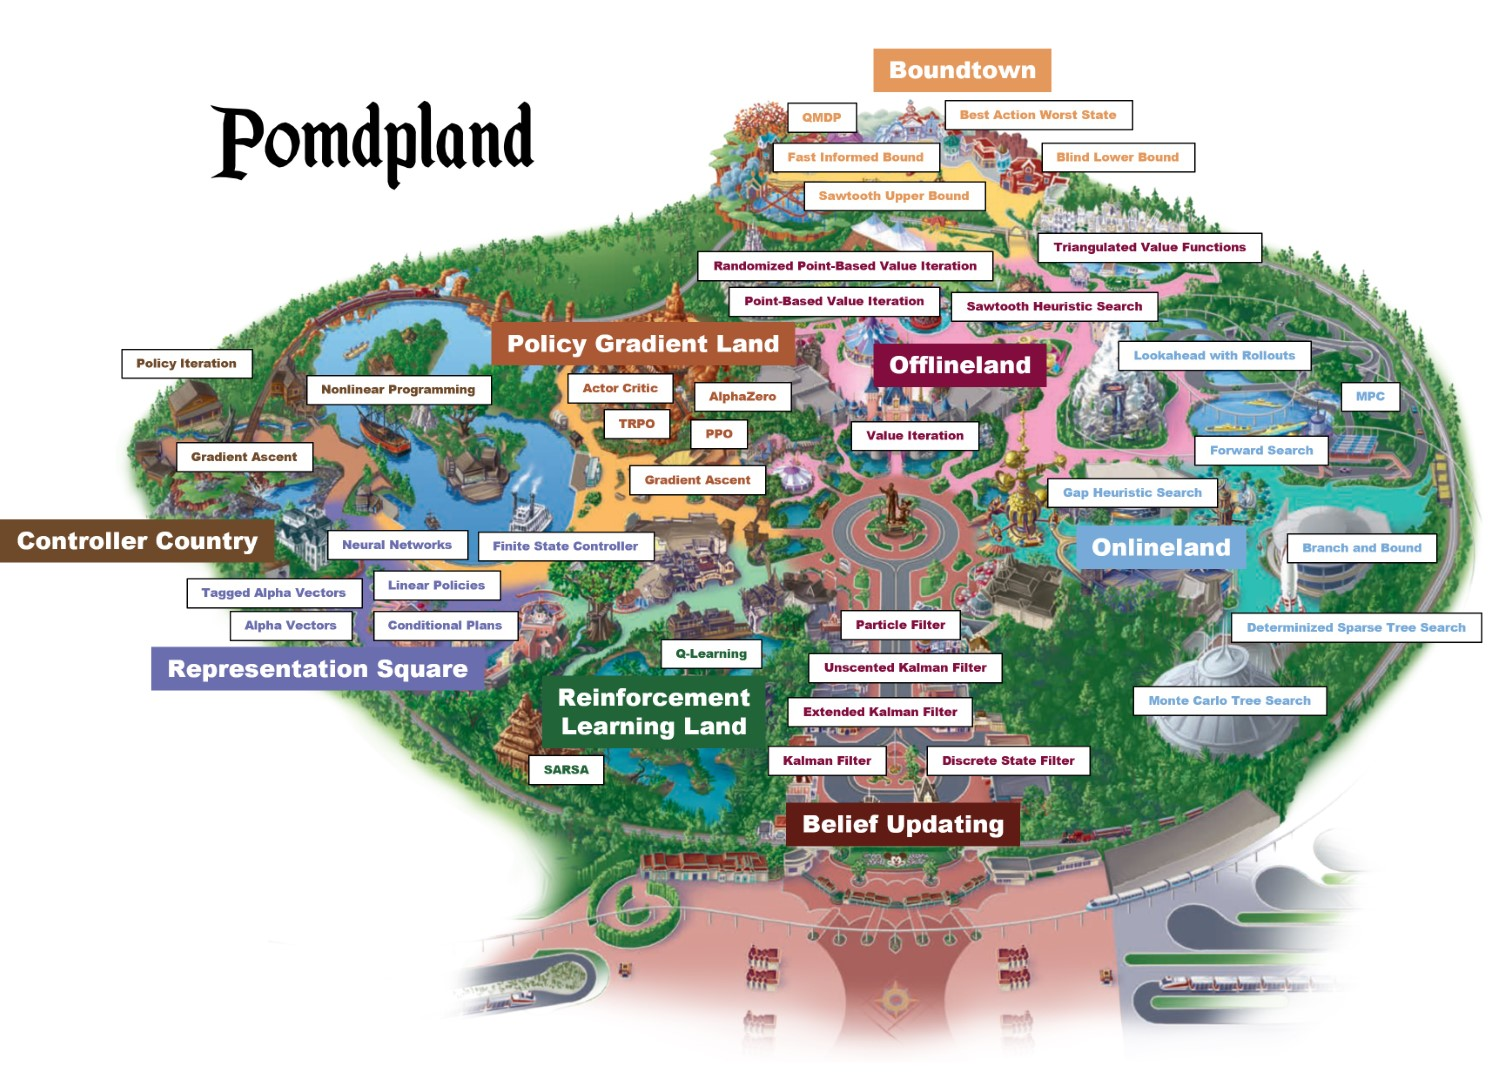
\includegraphics[width=\columnwidth]{pomdpland-small.jpeg}};
            \draw[red,ultra thick,rounded corners] (#1,#2) rectangle (#3,#4);
        \end{tikzpicture}
    
    \end{frame}
}

\title{A tour of Pomdpland}
\subtitle{Algorithms for sequential decision making under uncertainty}
\author{Mykel J. Kochenderfer}
\institute{Stanford University}

\begin{document}

\maketitle

\begin{frame}
    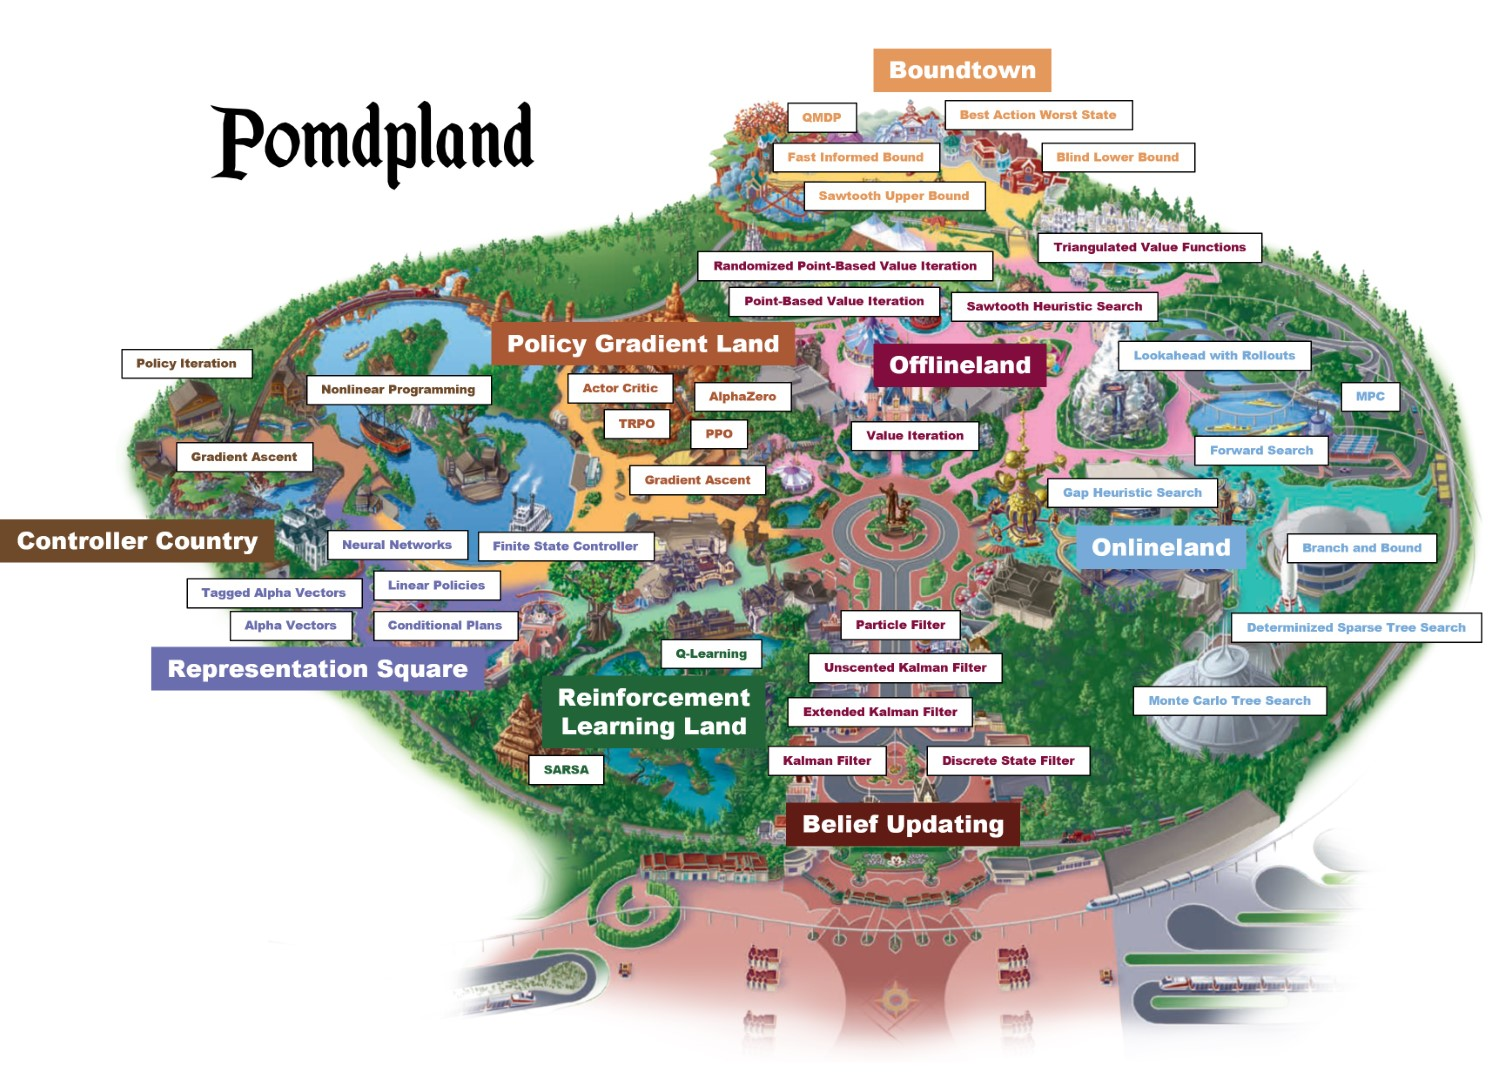
\includegraphics[width=\columnwidth]{pomdpland-small.jpeg}
\end{frame}

\begin{frame}{Sequential decision problems}
\begin{center}
    \begin{tikzpicture}
        \node [block,minimum width=3cm,minimum height=1cm] (env) {Environment};
        \node [block,minimum width=3cm,minimum height=1cm,right=of env] (ag) {Agent};
        \path [->,bend left=45] (env) edge node [above] {Observation ($o_t$)} (ag);
        \path [->,bend left=45] (ag) edge node [below] {Action ($a_t$)} (env);
        \end{tikzpicture}
\end{center}    
\end{frame}

\begin{frame}{POMDP definition}
    \centering
    \begin{tabular}{@{}lll@{}} \toprule
        Symbol & Description & Example \\ \midrule
        $\mathcal S$ & states & hungry ($h$), not hungry ($\neg h$)\\
        $\mathcal A$ & actions & feed ($f$), not feed ($\neg f$)\\
        $\mathcal O$ & observations & crying ($c$), not crying ($\neg c$)\\ \midrule
        $T(s' \mid s, a)$ & transition model & $T(h \mid \neg h, \neg f) = 0.2$\\
        $R(s, a)$ & reward model & $R(h, f) = -6$ \\
        $O(o \mid a, s')$ & observation model & $P(c \mid \neg f, h) = 0.9$ \\
        \bottomrule
    \end{tabular}   
\end{frame}

\begin{frame}{POMDP derived functions}
    \centering
    \begin{tabular}{@{}lll@{}}
        \toprule
        Symbol & Description \\ \midrule
        $b(s)$ & belief \\
        $U(b)$ & utility (or value) function \\
        $\pi(b)$ & policy \\        
        \bottomrule
    \end{tabular}
\end{frame}


\begin{frame}{Applications}
    \begin{enumerate}
        \item Aircraft collision avoidance
        \item Automated driving
        \item Breast cancer screening
        \item Financial consumption and portfolio allocation
        \item Distributed wildfire surveillance
        \item Mars science exploration
    \end{enumerate}
\end{frame}


\begin{frame}{Contributing disciplines}
    \begin{enumerate}
        \item Economics
        \item Psychology
        \item Neuroscience
        \item Computer science
        \item Engineering
        \item Mathematics
        \item Operations research
    \end{enumerate}
\end{frame}

\pomdpland{5.4}{1.5}{8}{3.5}

\begin{frame}{Beliefs}
    \begin{itemize}
        \item Discrete probability distribution (e.g., $\vec b = [0.2, 0.8]$)
        \item Parameters of a distribution (e.g., $b \sim \mathcal{N}(\vec \mu, \mat \Sigma)$)
        \item Collection of particles (e.g., $[3.4, 2.2, 9.6]$)
    \end{itemize}
    
\end{frame}

\begin{frame}{Belief updating}
    \begin{itemize}
        \item How do update our belief $b$ given that we took action $a$ and observed $o$?

        \item Bayes' rule tells us how to do this:
        \[b'(s') = O(o \mid a, s') \sum_{s} T(s' \mid s, a)b(s)\]
        
        \item We can use different approaches to define $b' = \text{Update}(b, a, o)$

        \begin{itemize}
            \item Discrete state filter
            \item Kalman filter
            \item Extended Kalman filter
            \item Unscented Kalman filter
            \item Particle filter
        \end{itemize}

    \end{itemize}

\end{frame}

\pomdpland{1}{2.6}{5}{4.2}

\begin{frame}{Linear policies}
    \begin{itemize}
        \item $\pi(b) = \mat{A} \hat{\vec{s}}$ where $\hat{\vec{s}}$ is the most likely state according to $b$
        \item Optimal for some problems (e.g., linear quadradic Gaussian)
        \item Good approximation for many other problems
    \end{itemize}
\end{frame}

\begin{frame}{Neural network policies}
    \begin{itemize}
        \item Handles very high dimensional problems (e.g., image inputs)
        \item Can use sequence of observations instead of beliefs
        \item May use LSTM, GRU, transformer architectures for tracking relevant past information
    \end{itemize}
\end{frame}

\begin{frame}{Conditional plans}
    Represent action to given any possible sequence of observations, up to some horizon

	\begin{center}
        \begin{tikzpicture}[>=stealth]
            \node (a1) at (0,0) {ignore};
            \node[anchor=west] (a2c) at (4, 1) {feed};
            \node[anchor=west] (a2n) at (4,-1) {ignore};
            \node[anchor=west] (a3cc) at (8, 1.5) {feed};
            \node[anchor=west] (a3nc) at (8, 0.5) {ignore};
            \node[anchor=west] (a3cn) at (8,-0.5) {feed};
            \node[anchor=west] (a3nn) at (8,-1.5) {ignore};
            \draw[->] (a1) [out=0,in=180] to (a2c);
            \node[rotate=30] at ($(a1)!0.55!(a2c) + (-0.1,0.25)$) {crying};
            \draw[->] (a1) [out=0,in=180] to (a2n);
            \node[rotate=-30] at ($(a1)!0.55!(a2n) - (0.3,0.2)$) {quiet};
    
            \draw[->] (a2c) [out=0,in=180] to (a3cc);
            \node[rotate=15] at ($(a2c)!0.55!(a3cc) + (-0.2,0.27)$) {crying};
            \draw[->] (a2c) [out=0,in=180] to (a3nc);
            \node[rotate=-16] at ($(a2c)!0.55!(a3nc) - (0.2,0.25)$) {quiet};
            \draw[->] (a2n) [out=0,in=180] to (a3cn);
            \node[rotate=18] at ($(a2n)!0.55!(a3cn) + (-0.2,0.22)$) {crying};
            \draw[->] (a2n) [out=0,in=180] to (a3nn);
            \node[rotate=-20] at ($(a2n)!0.55!(a3nn) - (0.2,0.2)$) {quiet};
        \end{tikzpicture}
        \end{center}
    

\end{frame}


\begin{frame}{Alpha vector policies}
    An \alert{alpha vector} $\vec \alpha$ defines a hyperplane over the belief space representing the value of executing a conditional plan $U(\vec b) = \vec \alpha^\transpose \vec b$

    \begin{tikzpicture}[]
        \begin{axis}[
          width=6cm, xmin=0, xmax=1, xlabel={$P(\text{hungry})$}, ylabel={$U(\vect b)$}, legend pos = {outer north east}
        ]
        
        \addplot+[
          solid_line, pastelRed
        ] coordinates {
          (0.0, -3.1744349999999995)
          (1.0, -25.192)
        };
        \addlegendentry{{}{given plan}}
        
        \addplot+[
          solid_line, pastelGreen
        ] coordinates {
          (0.0, -2.438999999999999)
          (1.0, -27.1)
        };
        \addlegendentry{{}{always ignore}}
        
        \addplot+[
          solid_line, pastelBlue
        ] coordinates {
          (0.0, -13.55)
          (1.0, -23.55)
        };
        \addlegendentry{{}{always feed}}
        
        \end{axis}
    \end{tikzpicture}
        


    \begin{itemize}
        \item  $U(b) = \max_{\vec \alpha \in \Gamma} \vec \alpha^\transpose \vec b$, where $\Gamma$ contains alpha vectors 
        \item $\pi(b) = \argmax_a [R(b,a) + \gamma \sum_o P(o \mid b, a)  U(\text{Update}(b, a, o))] $
    \end{itemize}

\end{frame}


\begin{frame}{Tagged alpha vector policies}
    A \alert{tagged alpha vector} is just an alpha vector labeled with the root action of the corresponding conditional plan

    \begin{tikzpicture}[]
        \begin{axis}[
          width=6cm, xmin=0, xmax=1, xlabel={$P(\text{hungry})$}, ylabel={$U(\vect b)$}, legend pos = {outer north east}
        ]
        
        \addplot+[
          solid_line, pastelRed
        ] coordinates {
          (0.0, -3.1744349999999995)
          (1.0, -25.192)
        };
        \addlegendentry{{}{ignore}}
        
        \addplot+[
          solid_line, pastelGreen
        ] coordinates {
          (0.0, -2.438999999999999)
          (1.0, -27.1)
        };
        \addlegendentry{{}{ignore}}
        
        \addplot+[
          solid_line, pastelBlue
        ] coordinates {
          (0.0, -13.55)
          (1.0, -23.55)
        };
        \addlegendentry{{}{feed}}
        
        \end{axis}
    \end{tikzpicture}

    Given our current belief, we find the maximizing alpha vector and execute the corresponding action
\end{frame}


\begin{frame}{Finite state controller policies}
    \begin{center}
    \begin{tikzpicture}[x=1cm, y=1cm]
        \node[minimum size=0.75cm, draw=black, fill=white, circle] (x1) {$x^1$};
        \node[minimum size=0.75cm, draw=black, fill=white, circle, right=2cm of x1] (x2) {$x^2$};
        \draw[->] (x1) to[bend left] node[above]{\small $o = \text{crying}$} (x2);
        \draw[->] (x2) to[bend left] node[below]{\small $o = \text{quiet}$} (x1);
        \path (x1) edge [loop left] node {\small $o = \text{quiet}$} (x2);
        \path (x2) edge [loop right] node {\small $o = \text{crying}$} (x2);
        \node[below left=0 and 0 of x1] {\small $\psi(\text{ignore} \mid x^1) = 1$};
        \node[below right=0 and 0 of x2] {\small $\psi(\text{feed} \mid x^2) = 1$};
    \end{tikzpicture}
    \end{center}
    \begin{itemize}
        \item Actions are associated with nodes
        \item Observations are associated with edges
        \item Associations can be stochastic
    \end{itemize}
\end{frame}

\pomdpland{5.4}{6.2}{9}{7.6}

\begin{frame}{QMDP upper bound}
    \begin{itemize}
        \item Assumes all uncertainty vanishes after first action
        \item Provides an upper bound
        \item Can be represented using one alpha vector per action
    \end{itemize}

    \begin{tikzpicture}[]
\begin{axis}[
  legend pos = {outer north east},
  width=8cm, height=5cm, xmin=0, xmax=1, ymax=0, ymin=-30, xlabel={$P(\text{hungry})$}, ylabel={$U(\vect b)$}
]

\addplot+[
  solid_line, pastelBlue!10.0
] coordinates {
  (0.0, 0.0)
  (0.01, -0.1)
  (0.02, -0.2)
  (0.03, -0.3)
  (0.04, -0.4)
  (0.05, -0.5)
  (0.06, -0.6)
  (0.07, -0.7000000000000001)
  (0.08, -0.8)
  (0.09, -0.8999999999999999)
  (0.1, -1.0)
  (0.11, -1.1)
  (0.12, -1.2)
  (0.13, -1.3)
  (0.14, -1.4000000000000001)
  (0.15, -1.5)
  (0.16, -1.6)
  (0.17, -1.7000000000000002)
  (0.18, -1.7999999999999998)
  (0.19, -1.9)
  (0.2, -2.0)
  (0.21, -2.1)
  (0.22, -2.2)
  (0.23, -2.3000000000000003)
  (0.24, -2.4)
  (0.25, -2.5)
  (0.26, -2.6)
  (0.27, -2.7)
  (0.28, -2.8000000000000003)
  (0.29, -2.9)
  (0.3, -3.0)
  (0.31, -3.1)
  (0.32, -3.2)
  (0.33, -3.3000000000000003)
  (0.34, -3.4000000000000004)
  (0.35, -3.5)
  (0.36, -3.5999999999999996)
  (0.37, -3.7)
  (0.38, -3.8)
  (0.39, -3.9000000000000004)
  (0.4, -4.0)
  (0.41, -4.1)
  (0.42, -4.2)
  (0.43, -4.3)
  (0.44, -4.4)
  (0.45, -4.5)
  (0.46, -4.6000000000000005)
  (0.47, -4.699999999999999)
  (0.48, -4.8)
  (0.49, -4.9)
  (0.5, -5.0)
  (0.51, -5.1)
  (0.52, -5.2)
  (0.53, -5.300000000000001)
  (0.54, -5.4)
  (0.55, -5.5)
  (0.56, -5.6000000000000005)
  (0.57, -5.699999999999999)
  (0.58, -5.8)
  (0.59, -5.8999999999999995)
  (0.6, -6.0)
  (0.61, -6.1)
  (0.62, -6.2)
  (0.63, -6.3)
  (0.64, -6.4)
  (0.65, -6.5)
  (0.66, -6.6000000000000005)
  (0.67, -6.7)
  (0.68, -6.800000000000001)
  (0.69, -6.8999999999999995)
  (0.7, -7.0)
  (0.71, -7.1)
  (0.72, -7.199999999999999)
  (0.73, -7.3)
  (0.74, -7.4)
  (0.75, -7.5)
  (0.76, -7.6)
  (0.77, -7.7)
  (0.78, -7.800000000000001)
  (0.79, -7.9)
  (0.8, -8.0)
  (0.81, -8.100000000000001)
  (0.82, -8.2)
  (0.83, -8.299999999999999)
  (0.84, -8.4)
  (0.85, -8.5)
  (0.86, -8.6)
  (0.87, -8.7)
  (0.88, -8.8)
  (0.89, -8.9)
  (0.9, -9.0)
  (0.91, -9.1)
  (0.92, -9.200000000000001)
  (0.93, -9.3)
  (0.94, -9.399999999999999)
  (0.95, -9.5)
  (0.96, -9.6)
  (0.97, -9.7)
  (0.98, -9.8)
  (0.99, -9.9)
  (1.0, -10.0)
};
\addlegendentry{{}{\num{1} iterations}}

\addplot+[
  solid_line, pastelBlue!19.0
] coordinates {
  (0.0, -0.8999999999999998)
  (0.01, -1.0809999999999997)
  (0.02, -1.2619999999999998)
  (0.03, -1.4429999999999998)
  (0.04, -1.6239999999999999)
  (0.05, -1.8049999999999997)
  (0.06, -1.9859999999999998)
  (0.07, -2.167)
  (0.08, -2.348)
  (0.09, -2.529)
  (0.1, -2.71)
  (0.11, -2.891)
  (0.12, -3.0719999999999996)
  (0.13, -3.253)
  (0.14, -3.434)
  (0.15, -3.6149999999999998)
  (0.16, -3.796)
  (0.17, -3.977)
  (0.18, -4.1579999999999995)
  (0.19, -4.3389999999999995)
  (0.2, -4.5200000000000005)
  (0.21, -4.701)
  (0.22, -4.882)
  (0.23, -5.063)
  (0.24, -5.244)
  (0.25, -5.425)
  (0.26, -5.606)
  (0.27, -5.787)
  (0.28, -5.968)
  (0.29, -6.148999999999999)
  (0.3, -6.329999999999999)
  (0.31, -6.511)
  (0.32, -6.692)
  (0.33, -6.873)
  (0.34, -7.054)
  (0.35, -7.234999999999999)
  (0.36, -7.4159999999999995)
  (0.37, -7.5969999999999995)
  (0.38, -7.778)
  (0.39, -7.959)
  (0.4, -8.14)
  (0.41, -8.321)
  (0.42, -8.501999999999999)
  (0.43, -8.683)
  (0.44, -8.864)
  (0.45, -9.045)
  (0.46, -9.226)
  (0.47, -9.407)
  (0.48, -9.588)
  (0.49, -9.769)
  (0.5, -9.95)
  (0.51, -10.1)
  (0.52, -10.2)
  (0.53, -10.3)
  (0.54, -10.4)
  (0.55, -10.5)
  (0.56, -10.600000000000001)
  (0.57, -10.7)
  (0.58, -10.799999999999999)
  (0.59, -10.9)
  (0.6, -11.0)
  (0.61, -11.1)
  (0.62, -11.2)
  (0.63, -11.3)
  (0.64, -11.4)
  (0.65, -11.5)
  (0.66, -11.6)
  (0.67, -11.700000000000001)
  (0.68, -11.8)
  (0.69, -11.899999999999999)
  (0.7, -12.0)
  (0.71, -12.1)
  (0.72, -12.2)
  (0.73, -12.3)
  (0.74, -12.4)
  (0.75, -12.5)
  (0.76, -12.6)
  (0.77, -12.7)
  (0.78, -12.8)
  (0.79, -12.9)
  (0.8, -13.0)
  (0.81, -13.100000000000001)
  (0.82, -13.2)
  (0.83, -13.299999999999999)
  (0.84, -13.4)
  (0.85, -13.5)
  (0.86, -13.6)
  (0.87, -13.7)
  (0.88, -13.8)
  (0.89, -13.9)
  (0.9, -14.0)
  (0.91, -14.1)
  (0.92, -14.200000000000001)
  (0.93, -14.3)
  (0.94, -14.399999999999999)
  (0.95, -14.5)
  (0.96, -14.6)
  (0.97, -14.7)
  (0.98, -14.8)
  (0.99, -14.9)
  (1.0, -15.0)
};
\addlegendentry{{}{\num{2} iterations}}

\addplot+[
  solid_line, pastelBlue!28.0
] coordinates {
  (0.0, -2.0789999999999997)
  (0.01, -2.2932099999999997)
  (0.02, -2.5074199999999998)
  (0.03, -2.7216299999999998)
  (0.04, -2.93584)
  (0.05, -3.15005)
  (0.06, -3.36426)
  (0.07, -3.57847)
  (0.08, -3.79268)
  (0.09, -4.006889999999999)
  (0.1, -4.2211)
  (0.11, -4.43531)
  (0.12, -4.64952)
  (0.13, -4.863729999999999)
  (0.14, -5.07794)
  (0.15, -5.2921499999999995)
  (0.16, -5.50636)
  (0.17, -5.7205699999999995)
  (0.18, -5.93478)
  (0.19, -6.1489899999999995)
  (0.2, -6.3632)
  (0.21, -6.5774099999999995)
  (0.22, -6.79162)
  (0.23, -7.00583)
  (0.24, -7.22004)
  (0.25, -7.43425)
  (0.26, -7.64846)
  (0.27, -7.8626700000000005)
  (0.28, -8.076880000000001)
  (0.29, -8.291089999999999)
  (0.3, -8.5053)
  (0.31, -8.71951)
  (0.32, -8.93372)
  (0.33, -9.11)
  (0.34, -9.209999999999999)
  (0.35, -9.31)
  (0.36, -9.41)
  (0.37, -9.51)
  (0.38, -9.61)
  (0.39, -9.71)
  (0.4, -9.81)
  (0.41, -9.91)
  (0.42, -10.01)
  (0.43, -10.11)
  (0.44, -10.21)
  (0.45, -10.31)
  (0.46, -10.41)
  (0.47, -10.51)
  (0.48, -10.61)
  (0.49, -10.709999999999999)
  (0.5, -10.81)
  (0.51, -10.91)
  (0.52, -11.01)
  (0.53, -11.110000000000001)
  (0.54, -11.21)
  (0.55, -11.31)
  (0.56, -11.41)
  (0.57, -11.51)
  (0.58, -11.61)
  (0.59, -11.709999999999999)
  (0.6, -11.81)
  (0.61, -11.91)
  (0.62, -12.01)
  (0.63, -12.11)
  (0.64, -12.21)
  (0.65, -12.31)
  (0.66, -12.41)
  (0.67, -12.51)
  (0.68, -12.610000000000001)
  (0.69, -12.709999999999999)
  (0.7, -12.81)
  (0.71, -12.91)
  (0.72, -13.01)
  (0.73, -13.11)
  (0.74, -13.21)
  (0.75, -13.31)
  (0.76, -13.41)
  (0.77, -13.51)
  (0.78, -13.610000000000001)
  (0.79, -13.71)
  (0.8, -13.81)
  (0.81, -13.91)
  (0.82, -14.01)
  (0.83, -14.11)
  (0.84, -14.21)
  (0.85, -14.31)
  (0.86, -14.41)
  (0.87, -14.51)
  (0.88, -14.610000000000001)
  (0.89, -14.71)
  (0.9, -14.81)
  (0.91, -14.91)
  (0.92, -15.010000000000002)
  (0.93, -15.110000000000001)
  (0.94, -15.209999999999999)
  (0.95, -15.31)
  (0.96, -15.41)
  (0.97, -15.51)
  (0.98, -15.61)
  (0.99, -15.71)
  (1.0, -15.81)
};
\addlegendentry{{}{\num{3} iterations}}

\addplot+[
  solid_line, pastelBlue!37.0
] coordinates {
  (0.0, -3.10689)
  (0.01, -3.3181111)
  (0.02, -3.5293322)
  (0.03, -3.7405532999999997)
  (0.04, -3.9517743999999997)
  (0.05, -4.1629955)
  (0.06, -4.3742166)
  (0.07, -4.5854377)
  (0.08, -4.7966587999999994)
  (0.09, -5.0078799)
  (0.1, -5.219101)
  (0.11, -5.4303221)
  (0.12, -5.6415432)
  (0.13, -5.8527643)
  (0.14, -6.0639854)
  (0.15, -6.2752064999999995)
  (0.16, -6.4864276)
  (0.17, -6.6976487)
  (0.18, -6.9088698)
  (0.19, -7.1200909)
  (0.2, -7.3313120000000005)
  (0.21, -7.5425331)
  (0.22, -7.7537541999999995)
  (0.23, -7.9649753)
  (0.24, -8.1761964)
  (0.25, -8.3874175)
  (0.26, -8.5986386)
  (0.27, -8.8098597)
  (0.28, -9.0210808)
  (0.29, -9.2323019)
  (0.3, -9.443522999999999)
  (0.31, -9.6547441)
  (0.32, -9.8659652)
  (0.33, -10.0771863)
  (0.34, -10.271099999999999)
  (0.35, -10.371099999999998)
  (0.36, -10.4711)
  (0.37, -10.5711)
  (0.38, -10.6711)
  (0.39, -10.7711)
  (0.4, -10.8711)
  (0.41, -10.9711)
  (0.42, -11.0711)
  (0.43, -11.1711)
  (0.44, -11.2711)
  (0.45, -11.3711)
  (0.46, -11.4711)
  (0.47, -11.5711)
  (0.48, -11.6711)
  (0.49, -11.771099999999999)
  (0.5, -11.871099999999998)
  (0.51, -11.9711)
  (0.52, -12.0711)
  (0.53, -12.1711)
  (0.54, -12.271099999999999)
  (0.55, -12.3711)
  (0.56, -12.4711)
  (0.57, -12.5711)
  (0.58, -12.6711)
  (0.59, -12.771099999999999)
  (0.6, -12.871099999999998)
  (0.61, -12.971099999999998)
  (0.62, -13.0711)
  (0.63, -13.1711)
  (0.64, -13.271099999999999)
  (0.65, -13.371099999999998)
  (0.66, -13.4711)
  (0.67, -13.5711)
  (0.68, -13.6711)
  (0.69, -13.771099999999999)
  (0.7, -13.871099999999998)
  (0.71, -13.971099999999998)
  (0.72, -14.071099999999998)
  (0.73, -14.1711)
  (0.74, -14.271099999999999)
  (0.75, -14.371099999999998)
  (0.76, -14.4711)
  (0.77, -14.5711)
  (0.78, -14.6711)
  (0.79, -14.771099999999999)
  (0.8, -14.871099999999998)
  (0.81, -14.9711)
  (0.82, -15.071099999999998)
  (0.83, -15.1711)
  (0.84, -15.271099999999999)
  (0.85, -15.371099999999998)
  (0.86, -15.471099999999998)
  (0.87, -15.571099999999998)
  (0.88, -15.6711)
  (0.89, -15.771099999999999)
  (0.9, -15.871099999999998)
  (0.91, -15.971099999999998)
  (0.92, -16.071099999999998)
  (0.93, -16.1711)
  (0.94, -16.271099999999997)
  (0.95, -16.3711)
  (0.96, -16.4711)
  (0.97, -16.571099999999998)
  (0.98, -16.6711)
  (0.99, -16.771099999999997)
  (1.0, -16.8711)
};
\addlegendentry{{}{\num{4} iterations}}

\addplot+[
  solid_line, pastelBlue!46.0
] coordinates {
  (0.0, -4.0349799)
  (0.01, -4.246470001)
  (0.02, -4.4579601019999995)
  (0.03, -4.669450202999999)
  (0.04, -4.880940304)
  (0.05, -5.092430405)
  (0.06, -5.303920505999999)
  (0.07, -5.515410607)
  (0.08, -5.7269007080000005)
  (0.09, -5.9383908089999995)
  (0.1, -6.14988091)
  (0.11, -6.361371011)
  (0.12, -6.572861112)
  (0.13, -6.784351213)
  (0.14, -6.995841314000001)
  (0.15, -7.207331415)
  (0.16, -7.418821516)
  (0.17, -7.630311617)
  (0.18, -7.841801718)
  (0.19, -8.053291819)
  (0.2, -8.26478192)
  (0.21, -8.476272021)
  (0.22, -8.687762122)
  (0.23, -8.899252223000001)
  (0.24, -9.110742324)
  (0.25, -9.322232425)
  (0.26, -9.533722526)
  (0.27, -9.745212627)
  (0.28, -9.956702728000002)
  (0.29, -10.168192828999999)
  (0.3, -10.37968293)
  (0.31, -10.591173031)
  (0.32, -10.802663132000001)
  (0.33, -11.014153233)
  (0.34, -11.196201)
  (0.35, -11.296201)
  (0.36, -11.396201)
  (0.37, -11.496201)
  (0.38, -11.596201)
  (0.39, -11.696201)
  (0.4, -11.796201)
  (0.41, -11.896201)
  (0.42, -11.996201)
  (0.43, -12.096201)
  (0.44, -12.196201)
  (0.45, -12.296201)
  (0.46, -12.396201)
  (0.47, -12.496201)
  (0.48, -12.596201)
  (0.49, -12.696201)
  (0.5, -12.796201)
  (0.51, -12.896201)
  (0.52, -12.996201000000001)
  (0.53, -13.096201)
  (0.54, -13.196201)
  (0.55, -13.296201)
  (0.56, -13.396201)
  (0.57, -13.496201)
  (0.58, -13.596200999999999)
  (0.59, -13.696201)
  (0.6, -13.796201)
  (0.61, -13.896201)
  (0.62, -13.996201)
  (0.63, -14.096201)
  (0.64, -14.196201)
  (0.65, -14.296201)
  (0.66, -14.396201)
  (0.67, -14.496201000000001)
  (0.68, -14.596201)
  (0.69, -14.696201)
  (0.7, -14.796201)
  (0.71, -14.896201)
  (0.72, -14.996201)
  (0.73, -15.096200999999999)
  (0.74, -15.196201)
  (0.75, -15.296201)
  (0.76, -15.396201)
  (0.77, -15.496201000000001)
  (0.78, -15.596201)
  (0.79, -15.696201)
  (0.8, -15.796201)
  (0.81, -15.896201000000001)
  (0.82, -15.996201)
  (0.83, -16.096201)
  (0.84, -16.196201)
  (0.85, -16.296201)
  (0.86, -16.396201)
  (0.87, -16.496201)
  (0.88, -16.596201)
  (0.89, -16.696201)
  (0.9, -16.796201)
  (0.91, -16.896201)
  (0.92, -16.996201)
  (0.93, -17.096201)
  (0.94, -17.196201)
  (0.95, -17.296201)
  (0.96, -17.396200999999998)
  (0.97, -17.496201)
  (0.98, -17.596201)
  (0.99, -17.696201)
  (1.0, -17.796201)
};
\addlegendentry{{}{\num{5} iterations}}

\addplot+[
  solid_line, pastelBlue!55.0
] coordinates {
  (0.0, -4.869991809)
  (0.01, -5.0814576999100005)
  (0.02, -5.29292359082)
  (0.03, -5.5043894817300005)
  (0.04, -5.71585537264)
  (0.05, -5.9273212635500006)
  (0.06, -6.138787154459999)
  (0.07, -6.350253045370001)
  (0.08, -6.56171893628)
  (0.09, -6.77318482719)
  (0.1, -6.9846507181)
  (0.11, -7.19611660901)
  (0.12, -7.40758249992)
  (0.13, -7.619048390830001)
  (0.14, -7.83051428174)
  (0.15, -8.04198017265)
  (0.16, -8.25344606356)
  (0.17, -8.46491195447)
  (0.18, -8.676377845380001)
  (0.19, -8.887843736290002)
  (0.2, -9.0993096272)
  (0.21, -9.31077551811)
  (0.22, -9.522241409020001)
  (0.23, -9.73370729993)
  (0.24, -9.94517319084)
  (0.25, -10.15663908175)
  (0.26, -10.368104972660001)
  (0.27, -10.57957086357)
  (0.28, -10.79103675448)
  (0.29, -11.002502645389999)
  (0.3, -11.2139685363)
  (0.31, -11.42543442721)
  (0.32, -11.63690031812)
  (0.33, -11.84836620903)
  (0.34, -12.031481909999998)
  (0.35, -12.131481909999998)
  (0.36, -12.23148191)
  (0.37, -12.331481909999999)
  (0.38, -12.431481909999999)
  (0.39, -12.531481909999998)
  (0.4, -12.63148191)
  (0.41, -12.73148191)
  (0.42, -12.831481909999999)
  (0.43, -12.931481909999999)
  (0.44, -13.03148191)
  (0.45, -13.13148191)
  (0.46, -13.23148191)
  (0.47, -13.331481909999999)
  (0.48, -13.431481909999999)
  (0.49, -13.531481909999998)
  (0.5, -13.631481909999998)
  (0.51, -13.73148191)
  (0.52, -13.831481909999999)
  (0.53, -13.931481909999999)
  (0.54, -14.03148191)
  (0.55, -14.13148191)
  (0.56, -14.23148191)
  (0.57, -14.331481909999999)
  (0.58, -14.431481909999999)
  (0.59, -14.531481909999998)
  (0.6, -14.631481909999998)
  (0.61, -14.73148191)
  (0.62, -14.831481909999999)
  (0.63, -14.931481909999999)
  (0.64, -15.031481909999998)
  (0.65, -15.131481909999998)
  (0.66, -15.23148191)
  (0.67, -15.331481909999999)
  (0.68, -15.431481909999999)
  (0.69, -15.531481909999998)
  (0.7, -15.631481909999998)
  (0.71, -15.731481909999998)
  (0.72, -15.831481909999997)
  (0.73, -15.931481909999999)
  (0.74, -16.031481909999997)
  (0.75, -16.131481909999998)
  (0.76, -16.23148191)
  (0.77, -16.331481909999997)
  (0.78, -16.43148191)
  (0.79, -16.53148191)
  (0.8, -16.631481909999998)
  (0.81, -16.73148191)
  (0.82, -16.831481909999997)
  (0.83, -16.93148191)
  (0.84, -17.031481909999997)
  (0.85, -17.131481909999998)
  (0.86, -17.23148191)
  (0.87, -17.331481909999997)
  (0.88, -17.43148191)
  (0.89, -17.53148191)
  (0.9, -17.631481909999998)
  (0.91, -17.73148191)
  (0.92, -17.831481909999997)
  (0.93, -17.93148191)
  (0.94, -18.031481909999997)
  (0.95, -18.131481909999998)
  (0.96, -18.23148191)
  (0.97, -18.331481909999997)
  (0.98, -18.43148191)
  (0.99, -18.531481909999997)
  (1.0, -18.631481909999998)
};
\addlegendentry{{}{\num{6} iterations}}

\addplot+[
  solid_line, pastelBlue!64.0
] coordinates {
  (0.0, -5.62152673719)
  (0.01, -5.832994807008101)
  (0.02, -6.044462876826199)
  (0.03, -6.2559309466443)
  (0.04, -6.4673990164624)
  (0.05, -6.6788670862804995)
  (0.06, -6.890335156098599)
  (0.07, -7.1018032259167)
  (0.08, -7.3132712957348)
  (0.09, -7.5247393655529)
  (0.1, -7.736207435371)
  (0.11, -7.9476755051891)
  (0.12, -8.1591435750072)
  (0.13, -8.3706116448253)
  (0.14, -8.582079714643399)
  (0.15, -8.7935477844615)
  (0.16, -9.005015854279598)
  (0.17, -9.2164839240977)
  (0.18, -9.4279519939158)
  (0.19, -9.6394200637339)
  (0.2, -9.850888133551999)
  (0.21, -10.0623562033701)
  (0.22, -10.273824273188199)
  (0.23, -10.4852923430063)
  (0.24, -10.6967604128244)
  (0.25, -10.9082284826425)
  (0.26, -11.1196965524606)
  (0.27, -11.331164622278699)
  (0.28, -11.542632692096799)
  (0.29, -11.754100761914898)
  (0.3, -11.965568831732998)
  (0.31, -12.1770369015511)
  (0.32, -12.3885049713692)
  (0.33, -12.5999730411873)
  (0.34, -12.782992628099999)
  (0.35, -12.8829926281)
  (0.36, -12.9829926281)
  (0.37, -13.0829926281)
  (0.38, -13.1829926281)
  (0.39, -13.2829926281)
  (0.4, -13.3829926281)
  (0.41, -13.4829926281)
  (0.42, -13.5829926281)
  (0.43, -13.6829926281)
  (0.44, -13.7829926281)
  (0.45, -13.8829926281)
  (0.46, -13.9829926281)
  (0.47, -14.0829926281)
  (0.48, -14.1829926281)
  (0.49, -14.282992628099999)
  (0.5, -14.382992628099998)
  (0.51, -14.4829926281)
  (0.52, -14.5829926281)
  (0.53, -14.6829926281)
  (0.54, -14.7829926281)
  (0.55, -14.8829926281)
  (0.56, -14.9829926281)
  (0.57, -15.082992628099998)
  (0.58, -15.1829926281)
  (0.59, -15.282992628099999)
  (0.6, -15.382992628099998)
  (0.61, -15.482992628099998)
  (0.62, -15.5829926281)
  (0.63, -15.6829926281)
  (0.64, -15.782992628099999)
  (0.65, -15.882992628099998)
  (0.66, -15.9829926281)
  (0.67, -16.082992628099998)
  (0.68, -16.1829926281)
  (0.69, -16.282992628099997)
  (0.7, -16.3829926281)
  (0.71, -16.4829926281)
  (0.72, -16.582992628099998)
  (0.73, -16.6829926281)
  (0.74, -16.7829926281)
  (0.75, -16.8829926281)
  (0.76, -16.9829926281)
  (0.77, -17.082992628099998)
  (0.78, -17.1829926281)
  (0.79, -17.2829926281)
  (0.8, -17.3829926281)
  (0.81, -17.4829926281)
  (0.82, -17.582992628099998)
  (0.83, -17.6829926281)
  (0.84, -17.782992628099997)
  (0.85, -17.8829926281)
  (0.86, -17.9829926281)
  (0.87, -18.082992628099998)
  (0.88, -18.1829926281)
  (0.89, -18.282992628099997)
  (0.9, -18.3829926281)
  (0.91, -18.4829926281)
  (0.92, -18.582992628099998)
  (0.93, -18.6829926281)
  (0.94, -18.782992628099997)
  (0.95, -18.8829926281)
  (0.96, -18.9829926281)
  (0.97, -19.082992628099998)
  (0.98, -19.1829926281)
  (0.99, -19.282992628099997)
  (1.0, -19.3829926281)
};
\addlegendentry{{}{\num{7} iterations}}

\addplot+[
  solid_line, pastelBlue!73.0
] coordinates {
  (0.0, -6.2979059936529)
  (0.01, -6.509373867369271)
  (0.02, -6.720841741085642)
  (0.03, -6.932309614802013)
  (0.04, -7.143777488518384)
  (0.05, -7.355245362234755)
  (0.06, -7.566713235951124)
  (0.07, -7.778181109667496)
  (0.08, -7.9896489833838675)
  (0.09, -8.201116857100239)
  (0.1, -8.41258473081661)
  (0.11, -8.62405260453298)
  (0.12, -8.835520478249352)
  (0.13, -9.046988351965723)
  (0.14, -9.258456225682094)
  (0.15, -9.469924099398463)
  (0.16, -9.681391973114835)
  (0.17, -9.892859846831207)
  (0.18, -10.104327720547579)
  (0.19, -10.31579559426395)
  (0.2, -10.52726346798032)
  (0.21, -10.738731341696692)
  (0.22, -10.950199215413063)
  (0.23, -11.161667089129432)
  (0.24, -11.373134962845803)
  (0.25, -11.584602836562174)
  (0.26, -11.796070710278546)
  (0.27, -12.007538583994917)
  (0.28, -12.219006457711288)
  (0.29, -12.430474331427659)
  (0.3, -12.64194220514403)
  (0.31, -12.853410078860401)
  (0.32, -13.064877952576772)
  (0.33, -13.276345826293143)
  (0.34, -13.459374063471)
  (0.35, -13.559374063471001)
  (0.36, -13.659374063471)
  (0.37, -13.759374063471)
  (0.38, -13.859374063471002)
  (0.39, -13.959374063471001)
  (0.4, -14.059374063471001)
  (0.41, -14.159374063471002)
  (0.42, -14.259374063471)
  (0.43, -14.359374063471002)
  (0.44, -14.459374063471001)
  (0.45, -14.559374063471001)
  (0.46, -14.659374063471002)
  (0.47, -14.759374063471)
  (0.48, -14.859374063471)
  (0.49, -14.959374063471001)
  (0.5, -15.059374063471001)
  (0.51, -15.159374063471)
  (0.52, -15.259374063471002)
  (0.53, -15.359374063471002)
  (0.54, -15.459374063471001)
  (0.55, -15.559374063471001)
  (0.56, -15.659374063471002)
  (0.57, -15.759374063471)
  (0.58, -15.859374063471)
  (0.59, -15.959374063471001)
  (0.6, -16.059374063471)
  (0.61, -16.159374063471002)
  (0.62, -16.259374063471)
  (0.63, -16.359374063471)
  (0.64, -16.459374063471)
  (0.65, -16.559374063471)
  (0.66, -16.659374063471002)
  (0.67, -16.759374063471)
  (0.68, -16.859374063471)
  (0.69, -16.959374063471)
  (0.7, -17.059374063471)
  (0.71, -17.159374063471)
  (0.72, -17.259374063471)
  (0.73, -17.359374063471)
  (0.74, -17.459374063471)
  (0.75, -17.559374063471)
  (0.76, -17.659374063471002)
  (0.77, -17.759374063471)
  (0.78, -17.859374063471)
  (0.79, -17.959374063471003)
  (0.8, -18.059374063471)
  (0.81, -18.159374063471002)
  (0.82, -18.259374063471)
  (0.83, -18.359374063471)
  (0.84, -18.459374063471)
  (0.85, -18.559374063471)
  (0.86, -18.659374063471002)
  (0.87, -18.759374063471)
  (0.88, -18.859374063471)
  (0.89, -18.959374063471)
  (0.9, -19.059374063471)
  (0.91, -19.159374063471002)
  (0.92, -19.259374063471)
  (0.93, -19.359374063471)
  (0.94, -19.459374063471)
  (0.95, -19.559374063471)
  (0.96, -19.659374063471002)
  (0.97, -19.759374063471)
  (0.98, -19.859374063471)
  (0.99, -19.959374063471)
  (1.0, -20.059374063471)
};
\addlegendentry{{}{\num{8} iterations}}

\addplot+[
  solid_line, pastelBlue!82.0
] coordinates {
  (0.0, -6.906647520571239)
  (0.01, -7.118115411936766)
  (0.02, -7.329583303302292)
  (0.03, -7.541051194667819)
  (0.04, -7.752519086033345)
  (0.05, -7.963986977398872)
  (0.06, -8.1754548687644)
  (0.07, -8.386922760129925)
  (0.08, -8.598390651495452)
  (0.09, -8.809858542860978)
  (0.1, -9.021326434226506)
  (0.11, -9.232794325592032)
  (0.12, -9.444262216957558)
  (0.13, -9.655730108323084)
  (0.14, -9.867197999688612)
  (0.15, -10.078665891054138)
  (0.16, -10.290133782419664)
  (0.17, -10.501601673785192)
  (0.18, -10.713069565150718)
  (0.19, -10.924537456516244)
  (0.2, -11.136005347881772)
  (0.21, -11.347473239247298)
  (0.22, -11.558941130612824)
  (0.23, -11.770409021978352)
  (0.24, -11.981876913343878)
  (0.25, -12.193344804709405)
  (0.26, -12.40481269607493)
  (0.27, -12.616280587440457)
  (0.28, -12.827748478805985)
  (0.29, -13.03921637017151)
  (0.3, -13.250684261537037)
  (0.31, -13.462152152902563)
  (0.32, -13.67362004426809)
  (0.33, -13.885087935633617)
  (0.34, -14.06811539428761)
  (0.35, -14.16811539428761)
  (0.36, -14.26811539428761)
  (0.37, -14.36811539428761)
  (0.38, -14.468115394287612)
  (0.39, -14.568115394287611)
  (0.4, -14.66811539428761)
  (0.41, -14.768115394287612)
  (0.42, -14.868115394287612)
  (0.43, -14.968115394287612)
  (0.44, -15.068115394287611)
  (0.45, -15.168115394287613)
  (0.46, -15.268115394287612)
  (0.47, -15.36811539428761)
  (0.48, -15.468115394287612)
  (0.49, -15.568115394287611)
  (0.5, -15.66811539428761)
  (0.51, -15.76811539428761)
  (0.52, -15.86811539428761)
  (0.53, -15.968115394287612)
  (0.54, -16.06811539428761)
  (0.55, -16.16811539428761)
  (0.56, -16.268115394287612)
  (0.57, -16.36811539428761)
  (0.58, -16.46811539428761)
  (0.59, -16.56811539428761)
  (0.6, -16.66811539428761)
  (0.61, -16.768115394287612)
  (0.62, -16.86811539428761)
  (0.63, -16.96811539428761)
  (0.64, -17.06811539428761)
  (0.65, -17.16811539428761)
  (0.66, -17.268115394287612)
  (0.67, -17.36811539428761)
  (0.68, -17.46811539428761)
  (0.69, -17.56811539428761)
  (0.7, -17.66811539428761)
  (0.71, -17.768115394287612)
  (0.72, -17.86811539428761)
  (0.73, -17.96811539428761)
  (0.74, -18.06811539428761)
  (0.75, -18.16811539428761)
  (0.76, -18.268115394287612)
  (0.77, -18.36811539428761)
  (0.78, -18.46811539428761)
  (0.79, -18.56811539428761)
  (0.8, -18.66811539428761)
  (0.81, -18.768115394287612)
  (0.82, -18.86811539428761)
  (0.83, -18.96811539428761)
  (0.84, -19.06811539428761)
  (0.85, -19.16811539428761)
  (0.86, -19.268115394287612)
  (0.87, -19.36811539428761)
  (0.88, -19.46811539428761)
  (0.89, -19.56811539428761)
  (0.9, -19.66811539428761)
  (0.91, -19.768115394287612)
  (0.92, -19.86811539428761)
  (0.93, -19.96811539428761)
  (0.94, -20.06811539428761)
  (0.95, -20.16811539428761)
  (0.96, -20.268115394287612)
  (0.97, -20.36811539428761)
  (0.98, -20.46811539428761)
  (0.99, -20.56811539428761)
  (1.0, -20.66811539428761)
};
\addlegendentry{{}{\num{9} iterations}}

\addplot+[
  solid_line, pastelBlue!91.0
] coordinates {
  (0.0, -7.454514877148588)
  (0.01, -7.665982766925691)
  (0.02, -7.877450656702793)
  (0.03, -8.088918546479896)
  (0.04, -8.300386436256998)
  (0.05, -8.5118543260341)
  (0.06, -8.723322215811203)
  (0.07, -8.934790105588306)
  (0.08, -9.14625799536541)
  (0.09, -9.357725885142512)
  (0.1, -9.569193774919615)
  (0.11, -9.780661664696717)
  (0.12, -9.99212955447382)
  (0.13, -10.203597444250923)
  (0.14, -10.415065334028025)
  (0.15, -10.626533223805128)
  (0.16, -10.83800111358223)
  (0.17, -11.049469003359333)
  (0.18, -11.260936893136437)
  (0.19, -11.47240478291354)
  (0.2, -11.683872672690642)
  (0.21, -11.895340562467744)
  (0.22, -12.106808452244847)
  (0.23, -12.31827634202195)
  (0.24, -12.529744231799052)
  (0.25, -12.741212121576154)
  (0.26, -12.952680011353257)
  (0.27, -13.16414790113036)
  (0.28, -13.375615790907462)
  (0.29, -13.587083680684563)
  (0.3, -13.798551570461667)
  (0.31, -14.01001946023877)
  (0.32, -14.221487350015872)
  (0.33, -14.432955239792975)
  (0.34, -14.615982768514115)
  (0.35, -14.715982768514115)
  (0.36, -14.815982768514116)
  (0.37, -14.915982768514116)
  (0.38, -15.015982768514116)
  (0.39, -15.115982768514115)
  (0.4, -15.215982768514117)
  (0.41, -15.315982768514116)
  (0.42, -15.415982768514116)
  (0.43, -15.515982768514116)
  (0.44, -15.615982768514117)
  (0.45, -15.715982768514117)
  (0.46, -15.815982768514116)
  (0.47, -15.915982768514116)
  (0.48, -16.015982768514117)
  (0.49, -16.115982768514115)
  (0.5, -16.215982768514117)
  (0.51, -16.315982768514115)
  (0.52, -16.415982768514116)
  (0.53, -16.515982768514117)
  (0.54, -16.615982768514115)
  (0.55, -16.715982768514117)
  (0.56, -16.815982768514115)
  (0.57, -16.915982768514116)
  (0.58, -17.015982768514114)
  (0.59, -17.115982768514115)
  (0.6, -17.215982768514117)
  (0.61, -17.315982768514115)
  (0.62, -17.415982768514116)
  (0.63, -17.515982768514117)
  (0.64, -17.615982768514115)
  (0.65, -17.715982768514117)
  (0.66, -17.815982768514115)
  (0.67, -17.915982768514116)
  (0.68, -18.015982768514117)
  (0.69, -18.115982768514115)
  (0.7, -18.215982768514117)
  (0.71, -18.315982768514115)
  (0.72, -18.415982768514116)
  (0.73, -18.515982768514117)
  (0.74, -18.615982768514115)
  (0.75, -18.715982768514117)
  (0.76, -18.815982768514115)
  (0.77, -18.915982768514116)
  (0.78, -19.015982768514117)
  (0.79, -19.115982768514115)
  (0.8, -19.215982768514117)
  (0.81, -19.315982768514118)
  (0.82, -19.415982768514116)
  (0.83, -19.515982768514117)
  (0.84, -19.615982768514115)
  (0.85, -19.715982768514117)
  (0.86, -19.815982768514118)
  (0.87, -19.915982768514116)
  (0.88, -20.015982768514117)
  (0.89, -20.115982768514115)
  (0.9, -20.215982768514117)
  (0.91, -20.315982768514118)
  (0.92, -20.415982768514116)
  (0.93, -20.515982768514117)
  (0.94, -20.615982768514115)
  (0.95, -20.715982768514117)
  (0.96, -20.815982768514115)
  (0.97, -20.915982768514116)
  (0.98, -21.015982768514117)
  (0.99, -21.115982768514115)
  (1.0, -21.215982768514117)
};
\addlegendentry{{}{\num{10} iterations}}

\addplot+[
  solid_line, pastelBlue
] coordinates {
  (0.0, -12.384945485175587)
  (0.01, -12.596413375083843)
  (0.02, -12.8078812649921)
  (0.03, -13.019349154900357)
  (0.04, -13.230817044808614)
  (0.05, -13.44228493471687)
  (0.06, -13.653752824625128)
  (0.07, -13.865220714533386)
  (0.08, -14.076688604441642)
  (0.09, -14.2881564943499)
  (0.1, -14.499624384258157)
  (0.11, -14.711092274166413)
  (0.12, -14.92256016407467)
  (0.13, -15.134028053982927)
  (0.14, -15.345495943891184)
  (0.15, -15.55696383379944)
  (0.16, -15.768431723707696)
  (0.17, -15.979899613615954)
  (0.18, -16.191367503524212)
  (0.19, -16.40283539343247)
  (0.2, -16.614303283340725)
  (0.21, -16.82577117324898)
  (0.22, -17.037239063157237)
  (0.23, -17.248706953065497)
  (0.24, -17.460174842973753)
  (0.25, -17.67164273288201)
  (0.26, -17.883110622790266)
  (0.27, -18.094578512698522)
  (0.28, -18.306046402606782)
  (0.29, -18.517514292515035)
  (0.3, -18.72898218242329)
  (0.31, -18.94045007233155)
  (0.32, -19.151917962239807)
  (0.33, -19.363385852148063)
  (0.34, -19.546413375083844)
  (0.35, -19.646413375083846)
  (0.36, -19.746413375083847)
  (0.37, -19.846413375083845)
  (0.38, -19.946413375083846)
  (0.39, -20.046413375083844)
  (0.4, -20.146413375083846)
  (0.41, -20.246413375083847)
  (0.42, -20.34641337508385)
  (0.43, -20.446413375083846)
  (0.44, -20.546413375083844)
  (0.45, -20.646413375083846)
  (0.46, -20.746413375083847)
  (0.47, -20.846413375083845)
  (0.48, -20.946413375083846)
  (0.49, -21.046413375083844)
  (0.5, -21.146413375083846)
  (0.51, -21.246413375083847)
  (0.52, -21.346413375083845)
  (0.53, -21.446413375083846)
  (0.54, -21.546413375083844)
  (0.55, -21.646413375083846)
  (0.56, -21.746413375083847)
  (0.57, -21.846413375083845)
  (0.58, -21.946413375083846)
  (0.59, -22.046413375083844)
  (0.6, -22.146413375083846)
  (0.61, -22.246413375083847)
  (0.62, -22.346413375083845)
  (0.63, -22.446413375083846)
  (0.64, -22.546413375083844)
  (0.65, -22.646413375083846)
  (0.66, -22.746413375083847)
  (0.67, -22.846413375083845)
  (0.68, -22.946413375083846)
  (0.69, -23.046413375083844)
  (0.7, -23.146413375083846)
  (0.71, -23.246413375083847)
  (0.72, -23.346413375083845)
  (0.73, -23.446413375083846)
  (0.74, -23.546413375083844)
  (0.75, -23.646413375083846)
  (0.76, -23.746413375083847)
  (0.77, -23.846413375083845)
  (0.78, -23.946413375083846)
  (0.79, -24.046413375083848)
  (0.8, -24.146413375083846)
  (0.81, -24.246413375083847)
  (0.82, -24.346413375083845)
  (0.83, -24.446413375083846)
  (0.84, -24.546413375083844)
  (0.85, -24.646413375083846)
  (0.86, -24.746413375083847)
  (0.87, -24.846413375083845)
  (0.88, -24.946413375083846)
  (0.89, -25.046413375083844)
  (0.9, -25.146413375083846)
  (0.91, -25.246413375083847)
  (0.92, -25.346413375083845)
  (0.93, -25.446413375083846)
  (0.94, -25.546413375083844)
  (0.95, -25.646413375083846)
  (0.96, -25.746413375083844)
  (0.97, -25.846413375083845)
  (0.98, -25.946413375083846)
  (0.99, -26.046413375083844)
  (1.0, -26.146413375083846)
};
\addlegendentry{{}{\num{100} iterations}}

\addplot+[
  solid_line, black
] coordinates {
  (0.0, -16.304979021966346)
  (0.01, -16.52443581310131)
  (0.02, -16.74389260423627)
  (0.03, -16.96334939537123)
  (0.04, -17.182806186506195)
  (0.05, -17.402262977641158)
  (0.06, -17.62171976877612)
  (0.07, -17.841176559911084)
  (0.08, -18.060633351046047)
  (0.09, -18.28009014218101)
  (0.1, -18.499546933315973)
  (0.11, -18.719003724450932)
  (0.12, -18.938460515585895)
  (0.13, -19.157917306720858)
  (0.14, -19.37737409785582)
  (0.15, -19.59683088899078)
  (0.16, -19.816287680125743)
  (0.17, -20.035744471260706)
  (0.18, -20.25520126239567)
  (0.19, -20.474658053530632)
  (0.2, -20.694114844665595)
  (0.21, -20.913571635800558)
  (0.22, -21.13302842693552)
  (0.23, -21.352485218070484)
  (0.24, -21.571942009205443)
  (0.25, -21.791398800340406)
  (0.26, -22.01085559147537)
  (0.27, -22.230312382610332)
  (0.28, -22.449769173745295)
  (0.29, -22.57443069235409)
  (0.3, -22.67443069235409)
  (0.31, -22.774430692354088)
  (0.32, -22.87443069235409)
  (0.33, -22.974430692354087)
  (0.34, -23.07443069235409)
  (0.35, -23.17443069235409)
  (0.36, -23.274430692354088)
  (0.37, -23.37443069235409)
  (0.38, -23.47443069235409)
  (0.39, -23.57443069235409)
  (0.4, -23.67443069235409)
  (0.41, -23.77443069235409)
  (0.42, -23.87443069235409)
  (0.43, -23.97443069235409)
  (0.44, -24.074430692354092)
  (0.45, -24.17443069235409)
  (0.46, -24.27443069235409)
  (0.47, -24.37443069235409)
  (0.48, -24.47443069235409)
  (0.49, -24.57443069235409)
  (0.5, -24.67443069235409)
  (0.51, -24.77443069235409)
  (0.52, -24.87443069235409)
  (0.53, -24.97443069235409)
  (0.54, -25.074430692354092)
  (0.55, -25.17443069235409)
  (0.56, -25.27443069235409)
  (0.57, -25.37443069235409)
  (0.58, -25.47443069235409)
  (0.59, -25.57443069235409)
  (0.6, -25.67443069235409)
  (0.61, -25.77443069235409)
  (0.62, -25.87443069235409)
  (0.63, -25.97443069235409)
  (0.64, -26.07443069235409)
  (0.65, -26.17443069235409)
  (0.66, -26.27443069235409)
  (0.67, -26.37443069235409)
  (0.68, -26.47443069235409)
  (0.69, -26.57443069235409)
  (0.7, -26.67443069235409)
  (0.71, -26.774430692354088)
  (0.72, -26.87443069235409)
  (0.73, -26.97443069235409)
  (0.74, -27.07443069235409)
  (0.75, -27.17443069235409)
  (0.76, -27.27443069235409)
  (0.77, -27.37443069235409)
  (0.78, -27.47443069235409)
  (0.79, -27.574430692354092)
  (0.8, -27.67443069235409)
  (0.81, -27.77443069235409)
  (0.82, -27.87443069235409)
  (0.83, -27.97443069235409)
  (0.84, -28.07443069235409)
  (0.85, -28.17443069235409)
  (0.86, -28.27443069235409)
  (0.87, -28.37443069235409)
  (0.88, -28.47443069235409)
  (0.89, -28.57443069235409)
  (0.9, -28.67443069235409)
  (0.91, -28.77443069235409)
  (0.92, -28.87443069235409)
  (0.93, -28.97443069235409)
  (0.94, -29.07443069235409)
  (0.95, -29.17443069235409)
  (0.96, -29.27443069235409)
  (0.97, -29.37443069235409)
  (0.98, -29.47443069235409)
  (0.99, -29.57443069235409)
  (1.0, -29.67443069235409)
};
\addlegendentry{{}{optimal}}

\end{axis}
\end{tikzpicture}


    
\end{frame}

\begin{frame}{FIB upper bownd}
    \begin{itemize}
        \item Upper bound no less tight (and generally tighter) than QMDP
        \item One alpha vector per action
        \item Uses observation model in calculations
        \item More expensive than QMDP, but tightness may be worthwhile
    \end{itemize}

    \begin{tikzpicture}[]
\begin{axis}[
  legend pos = {outer north east},
  width=8cm, height=5cm, xmin=0, xmax=1, ymax=0, ymin=-30, xlabel={$P(\text{hungry})$}, ylabel={$U(\vect b)$}
]

\addplot+[
  solid_line, pastelRed!10.0
] coordinates {
  (0.0, 0.0)
  (0.01, -0.1)
  (0.02, -0.2)
  (0.03, -0.3)
  (0.04, -0.4)
  (0.05, -0.5)
  (0.06, -0.6)
  (0.07, -0.7000000000000001)
  (0.08, -0.8)
  (0.09, -0.8999999999999999)
  (0.1, -1.0)
  (0.11, -1.1)
  (0.12, -1.2)
  (0.13, -1.3)
  (0.14, -1.4000000000000001)
  (0.15, -1.5)
  (0.16, -1.6)
  (0.17, -1.7000000000000002)
  (0.18, -1.7999999999999998)
  (0.19, -1.9)
  (0.2, -2.0)
  (0.21, -2.1)
  (0.22, -2.2)
  (0.23, -2.3000000000000003)
  (0.24, -2.4)
  (0.25, -2.5)
  (0.26, -2.6)
  (0.27, -2.7)
  (0.28, -2.8000000000000003)
  (0.29, -2.9)
  (0.3, -3.0)
  (0.31, -3.1)
  (0.32, -3.2)
  (0.33, -3.3000000000000003)
  (0.34, -3.4000000000000004)
  (0.35, -3.5)
  (0.36, -3.5999999999999996)
  (0.37, -3.7)
  (0.38, -3.8)
  (0.39, -3.9000000000000004)
  (0.4, -4.0)
  (0.41, -4.1)
  (0.42, -4.2)
  (0.43, -4.3)
  (0.44, -4.4)
  (0.45, -4.5)
  (0.46, -4.6000000000000005)
  (0.47, -4.699999999999999)
  (0.48, -4.8)
  (0.49, -4.9)
  (0.5, -5.0)
  (0.51, -5.1)
  (0.52, -5.2)
  (0.53, -5.300000000000001)
  (0.54, -5.4)
  (0.55, -5.5)
  (0.56, -5.6000000000000005)
  (0.57, -5.699999999999999)
  (0.58, -5.8)
  (0.59, -5.8999999999999995)
  (0.6, -6.0)
  (0.61, -6.1)
  (0.62, -6.2)
  (0.63, -6.3)
  (0.64, -6.4)
  (0.65, -6.5)
  (0.66, -6.6000000000000005)
  (0.67, -6.7)
  (0.68, -6.800000000000001)
  (0.69, -6.8999999999999995)
  (0.7, -7.0)
  (0.71, -7.1)
  (0.72, -7.199999999999999)
  (0.73, -7.3)
  (0.74, -7.4)
  (0.75, -7.5)
  (0.76, -7.6)
  (0.77, -7.7)
  (0.78, -7.800000000000001)
  (0.79, -7.9)
  (0.8, -8.0)
  (0.81, -8.100000000000001)
  (0.82, -8.2)
  (0.83, -8.299999999999999)
  (0.84, -8.4)
  (0.85, -8.5)
  (0.86, -8.6)
  (0.87, -8.7)
  (0.88, -8.8)
  (0.89, -8.9)
  (0.9, -9.0)
  (0.91, -9.1)
  (0.92, -9.200000000000001)
  (0.93, -9.3)
  (0.94, -9.399999999999999)
  (0.95, -9.5)
  (0.96, -9.6)
  (0.97, -9.7)
  (0.98, -9.8)
  (0.99, -9.9)
  (1.0, -10.0)
};
\addlegendentry{{}{\num{1} iterations}}

\addplot+[
  solid_line, pastelRed!19.0
] coordinates {
  (0.0, -0.8999999999999998)
  (0.01, -1.0809999999999997)
  (0.02, -1.2619999999999998)
  (0.03, -1.4429999999999998)
  (0.04, -1.6239999999999999)
  (0.05, -1.8049999999999997)
  (0.06, -1.9859999999999998)
  (0.07, -2.167)
  (0.08, -2.348)
  (0.09, -2.529)
  (0.1, -2.71)
  (0.11, -2.891)
  (0.12, -3.0719999999999996)
  (0.13, -3.253)
  (0.14, -3.434)
  (0.15, -3.6149999999999998)
  (0.16, -3.796)
  (0.17, -3.977)
  (0.18, -4.1579999999999995)
  (0.19, -4.3389999999999995)
  (0.2, -4.5200000000000005)
  (0.21, -4.701)
  (0.22, -4.882)
  (0.23, -5.063)
  (0.24, -5.244)
  (0.25, -5.425)
  (0.26, -5.606)
  (0.27, -5.787)
  (0.28, -5.968)
  (0.29, -6.148999999999999)
  (0.3, -6.329999999999999)
  (0.31, -6.511)
  (0.32, -6.692)
  (0.33, -6.873)
  (0.34, -7.054)
  (0.35, -7.234999999999999)
  (0.36, -7.4159999999999995)
  (0.37, -7.5969999999999995)
  (0.38, -7.778)
  (0.39, -7.959)
  (0.4, -8.14)
  (0.41, -8.321)
  (0.42, -8.501999999999999)
  (0.43, -8.683)
  (0.44, -8.864)
  (0.45, -9.045)
  (0.46, -9.226)
  (0.47, -9.407)
  (0.48, -9.588)
  (0.49, -9.769)
  (0.5, -9.95)
  (0.51, -10.1)
  (0.52, -10.2)
  (0.53, -10.3)
  (0.54, -10.4)
  (0.55, -10.5)
  (0.56, -10.600000000000001)
  (0.57, -10.7)
  (0.58, -10.799999999999999)
  (0.59, -10.9)
  (0.6, -11.0)
  (0.61, -11.1)
  (0.62, -11.2)
  (0.63, -11.3)
  (0.64, -11.4)
  (0.65, -11.5)
  (0.66, -11.6)
  (0.67, -11.700000000000001)
  (0.68, -11.8)
  (0.69, -11.899999999999999)
  (0.7, -12.0)
  (0.71, -12.1)
  (0.72, -12.2)
  (0.73, -12.3)
  (0.74, -12.4)
  (0.75, -12.5)
  (0.76, -12.6)
  (0.77, -12.7)
  (0.78, -12.8)
  (0.79, -12.9)
  (0.8, -13.0)
  (0.81, -13.100000000000001)
  (0.82, -13.2)
  (0.83, -13.299999999999999)
  (0.84, -13.4)
  (0.85, -13.5)
  (0.86, -13.6)
  (0.87, -13.7)
  (0.88, -13.8)
  (0.89, -13.9)
  (0.9, -14.0)
  (0.91, -14.1)
  (0.92, -14.200000000000001)
  (0.93, -14.3)
  (0.94, -14.399999999999999)
  (0.95, -14.5)
  (0.96, -14.6)
  (0.97, -14.7)
  (0.98, -14.8)
  (0.99, -14.9)
  (1.0, -15.0)
};
\addlegendentry{{}{\num{2} iterations}}

\addplot+[
  solid_line, pastelRed!28.0
] coordinates {
  (0.0, -2.438999999999999)
  (0.01, -2.649609999999999)
  (0.02, -2.8602199999999995)
  (0.03, -3.070829999999999)
  (0.04, -3.281439999999999)
  (0.05, -3.4920499999999994)
  (0.06, -3.7026599999999994)
  (0.07, -3.913269999999999)
  (0.08, -4.12388)
  (0.09, -4.33449)
  (0.1, -4.5451)
  (0.11, -4.75571)
  (0.12, -4.96632)
  (0.13, -5.17693)
  (0.14, -5.3875399999999996)
  (0.15, -5.598149999999999)
  (0.16, -5.8087599999999995)
  (0.17, -6.019369999999999)
  (0.18, -6.229979999999999)
  (0.19, -6.440589999999999)
  (0.2, -6.651199999999999)
  (0.21, -6.861809999999999)
  (0.22, -7.072419999999999)
  (0.23, -7.283029999999999)
  (0.24, -7.493639999999999)
  (0.25, -7.704249999999999)
  (0.26, -7.91486)
  (0.27, -8.12547)
  (0.28, -8.33608)
  (0.29, -8.546689999999998)
  (0.3, -8.757299999999999)
  (0.31, -8.91)
  (0.32, -9.01)
  (0.33, -9.11)
  (0.34, -9.209999999999999)
  (0.35, -9.31)
  (0.36, -9.41)
  (0.37, -9.51)
  (0.38, -9.61)
  (0.39, -9.71)
  (0.4, -9.81)
  (0.41, -9.91)
  (0.42, -10.01)
  (0.43, -10.11)
  (0.44, -10.21)
  (0.45, -10.31)
  (0.46, -10.41)
  (0.47, -10.51)
  (0.48, -10.61)
  (0.49, -10.709999999999999)
  (0.5, -10.81)
  (0.51, -10.91)
  (0.52, -11.01)
  (0.53, -11.110000000000001)
  (0.54, -11.21)
  (0.55, -11.31)
  (0.56, -11.41)
  (0.57, -11.51)
  (0.58, -11.61)
  (0.59, -11.709999999999999)
  (0.6, -11.81)
  (0.61, -11.91)
  (0.62, -12.01)
  (0.63, -12.11)
  (0.64, -12.21)
  (0.65, -12.31)
  (0.66, -12.41)
  (0.67, -12.51)
  (0.68, -12.610000000000001)
  (0.69, -12.709999999999999)
  (0.7, -12.81)
  (0.71, -12.91)
  (0.72, -13.01)
  (0.73, -13.11)
  (0.74, -13.21)
  (0.75, -13.31)
  (0.76, -13.41)
  (0.77, -13.51)
  (0.78, -13.610000000000001)
  (0.79, -13.71)
  (0.8, -13.81)
  (0.81, -13.91)
  (0.82, -14.01)
  (0.83, -14.11)
  (0.84, -14.21)
  (0.85, -14.31)
  (0.86, -14.41)
  (0.87, -14.51)
  (0.88, -14.610000000000001)
  (0.89, -14.71)
  (0.9, -14.81)
  (0.91, -14.91)
  (0.92, -15.010000000000002)
  (0.93, -15.110000000000001)
  (0.94, -15.209999999999999)
  (0.95, -15.31)
  (0.96, -15.41)
  (0.97, -15.51)
  (0.98, -15.61)
  (0.99, -15.71)
  (1.0, -15.81)
};
\addlegendentry{{}{\num{3} iterations}}

\addplot+[
  solid_line, pastelRed!37.0
] coordinates {
  (0.0, -3.8099609999999995)
  (0.01, -4.014151389999999)
  (0.02, -4.218341779999999)
  (0.03, -4.422532169999999)
  (0.04, -4.626722559999999)
  (0.05, -4.830912949999999)
  (0.06, -5.035103339999999)
  (0.07, -5.239293729999999)
  (0.08, -5.44348412)
  (0.09, -5.64767451)
  (0.1, -5.8518649)
  (0.11, -6.05605529)
  (0.12, -6.26024568)
  (0.13, -6.46443607)
  (0.14, -6.66862646)
  (0.15, -6.8728168499999995)
  (0.16, -7.0770072399999995)
  (0.17, -7.281197629999999)
  (0.18, -7.485388019999999)
  (0.19, -7.689578409999999)
  (0.2, -7.8937688)
  (0.21, -8.09795919)
  (0.22, -8.30214958)
  (0.23, -8.506339969999999)
  (0.24, -8.71053036)
  (0.25, -8.914720749999999)
  (0.26, -9.11891114)
  (0.27, -9.32310153)
  (0.28, -9.52729192)
  (0.29, -9.731482309999999)
  (0.3, -9.9356727)
  (0.31, -10.139863089999999)
  (0.32, -10.34405348)
  (0.33, -10.495099999999999)
  (0.34, -10.595099999999999)
  (0.35, -10.695099999999998)
  (0.36, -10.7951)
  (0.37, -10.8951)
  (0.38, -10.995099999999999)
  (0.39, -11.095099999999999)
  (0.4, -11.1951)
  (0.41, -11.2951)
  (0.42, -11.3951)
  (0.43, -11.495099999999999)
  (0.44, -11.5951)
  (0.45, -11.6951)
  (0.46, -11.7951)
  (0.47, -11.8951)
  (0.48, -11.995099999999999)
  (0.49, -12.095099999999999)
  (0.5, -12.1951)
  (0.51, -12.2951)
  (0.52, -12.3951)
  (0.53, -12.4951)
  (0.54, -12.5951)
  (0.55, -12.6951)
  (0.56, -12.7951)
  (0.57, -12.8951)
  (0.58, -12.995099999999999)
  (0.59, -13.095099999999999)
  (0.6, -13.1951)
  (0.61, -13.2951)
  (0.62, -13.3951)
  (0.63, -13.4951)
  (0.64, -13.5951)
  (0.65, -13.6951)
  (0.66, -13.7951)
  (0.67, -13.8951)
  (0.68, -13.9951)
  (0.69, -14.095099999999999)
  (0.7, -14.1951)
  (0.71, -14.2951)
  (0.72, -14.3951)
  (0.73, -14.495099999999999)
  (0.74, -14.5951)
  (0.75, -14.6951)
  (0.76, -14.7951)
  (0.77, -14.8951)
  (0.78, -14.9951)
  (0.79, -15.0951)
  (0.8, -15.1951)
  (0.81, -15.2951)
  (0.82, -15.3951)
  (0.83, -15.495099999999999)
  (0.84, -15.5951)
  (0.85, -15.6951)
  (0.86, -15.7951)
  (0.87, -15.8951)
  (0.88, -15.9951)
  (0.89, -16.0951)
  (0.9, -16.1951)
  (0.91, -16.2951)
  (0.92, -16.3951)
  (0.93, -16.4951)
  (0.94, -16.5951)
  (0.95, -16.6951)
  (0.96, -16.795099999999998)
  (0.97, -16.8951)
  (0.98, -16.9951)
  (0.99, -17.0951)
  (1.0, -17.1951)
};
\addlegendentry{{}{\num{4} iterations}}

\addplot+[
  solid_line, pastelRed!46.0
] coordinates {
  (0.0, -5.034433869)
  (0.01, -5.23884543031)
  (0.02, -5.44325699162)
  (0.03, -5.647668552929999)
  (0.04, -5.85208011424)
  (0.05, -6.056491675549999)
  (0.06, -6.26090323686)
  (0.07, -6.46531479817)
  (0.08, -6.66972635948)
  (0.09, -6.87413792079)
  (0.1, -7.078549482100001)
  (0.11, -7.282961043409999)
  (0.12, -7.48737260472)
  (0.13, -7.69178416603)
  (0.14, -7.89619572734)
  (0.15, -8.10060728865)
  (0.16, -8.30501884996)
  (0.17, -8.50943041127)
  (0.18, -8.71384197258)
  (0.19, -8.91825353389)
  (0.2, -9.1226650952)
  (0.21, -9.32707665651)
  (0.22, -9.53148821782)
  (0.23, -9.735899779130001)
  (0.24, -9.94031134044)
  (0.25, -10.14472290175)
  (0.26, -10.34913446306)
  (0.27, -10.55354602437)
  (0.28, -10.75795758568)
  (0.29, -10.96236914699)
  (0.3, -11.1667807083)
  (0.31, -11.371192269609999)
  (0.32, -11.57560383092)
  (0.33, -11.7289649)
  (0.34, -11.8289649)
  (0.35, -11.9289649)
  (0.36, -12.0289649)
  (0.37, -12.1289649)
  (0.38, -12.228964900000001)
  (0.39, -12.3289649)
  (0.4, -12.4289649)
  (0.41, -12.5289649)
  (0.42, -12.628964900000001)
  (0.43, -12.728964900000001)
  (0.44, -12.8289649)
  (0.45, -12.9289649)
  (0.46, -13.0289649)
  (0.47, -13.1289649)
  (0.48, -13.2289649)
  (0.49, -13.3289649)
  (0.5, -13.4289649)
  (0.51, -13.5289649)
  (0.52, -13.628964900000001)
  (0.53, -13.728964900000001)
  (0.54, -13.8289649)
  (0.55, -13.9289649)
  (0.56, -14.0289649)
  (0.57, -14.1289649)
  (0.58, -14.2289649)
  (0.59, -14.3289649)
  (0.6, -14.4289649)
  (0.61, -14.5289649)
  (0.62, -14.6289649)
  (0.63, -14.728964900000001)
  (0.64, -14.8289649)
  (0.65, -14.9289649)
  (0.66, -15.0289649)
  (0.67, -15.128964900000001)
  (0.68, -15.228964900000001)
  (0.69, -15.3289649)
  (0.7, -15.4289649)
  (0.71, -15.5289649)
  (0.72, -15.6289649)
  (0.73, -15.7289649)
  (0.74, -15.8289649)
  (0.75, -15.9289649)
  (0.76, -16.028964900000002)
  (0.77, -16.1289649)
  (0.78, -16.2289649)
  (0.79, -16.328964900000003)
  (0.8, -16.4289649)
  (0.81, -16.528964900000002)
  (0.82, -16.6289649)
  (0.83, -16.7289649)
  (0.84, -16.8289649)
  (0.85, -16.9289649)
  (0.86, -17.028964900000002)
  (0.87, -17.1289649)
  (0.88, -17.2289649)
  (0.89, -17.3289649)
  (0.9, -17.4289649)
  (0.91, -17.528964900000002)
  (0.92, -17.6289649)
  (0.93, -17.7289649)
  (0.94, -17.8289649)
  (0.95, -17.9289649)
  (0.96, -18.0289649)
  (0.97, -18.1289649)
  (0.98, -18.2289649)
  (0.99, -18.3289649)
  (1.0, -18.4289649)
};
\addlegendentry{{}{\num{5} iterations}}

\addplot+[
  solid_line, pastelRed!55.0
] coordinates {
  (0.0, -6.138294540201)
  (0.01, -6.342772278898989)
  (0.02, -6.54725001759698)
  (0.03, -6.75172775629497)
  (0.04, -6.956205494992959)
  (0.05, -7.160683233690949)
  (0.06, -7.3651609723889395)
  (0.07, -7.569638711086929)
  (0.08, -7.77411644978492)
  (0.09, -7.9785941884829095)
  (0.1, -8.1830719271809)
  (0.11, -8.38754966587889)
  (0.12, -8.59202740457688)
  (0.13, -8.796505143274869)
  (0.14, -9.00098288197286)
  (0.15, -9.20546062067085)
  (0.16, -9.409938359368839)
  (0.17, -9.61441609806683)
  (0.18, -9.81889383676482)
  (0.19, -10.02337157546281)
  (0.2, -10.2278493141608)
  (0.21, -10.43232705285879)
  (0.22, -10.63680479155678)
  (0.23, -10.84128253025477)
  (0.24, -11.04576026895276)
  (0.25, -11.25023800765075)
  (0.26, -11.45471574634874)
  (0.27, -11.65919348504673)
  (0.28, -11.86367122374472)
  (0.29, -12.06814896244271)
  (0.3, -12.2726267011407)
  (0.31, -12.477104439838689)
  (0.32, -12.68158217853668)
  (0.33, -12.8309904821)
  (0.34, -12.9309904821)
  (0.35, -13.0309904821)
  (0.36, -13.130990482100001)
  (0.37, -13.230990482100001)
  (0.38, -13.3309904821)
  (0.39, -13.4309904821)
  (0.4, -13.5309904821)
  (0.41, -13.630990482100001)
  (0.42, -13.730990482100001)
  (0.43, -13.8309904821)
  (0.44, -13.9309904821)
  (0.45, -14.030990482100002)
  (0.46, -14.130990482100001)
  (0.47, -14.230990482100001)
  (0.48, -14.3309904821)
  (0.49, -14.4309904821)
  (0.5, -14.530990482100002)
  (0.51, -14.630990482100001)
  (0.52, -14.730990482100001)
  (0.53, -14.8309904821)
  (0.54, -14.930990482100002)
  (0.55, -15.030990482100002)
  (0.56, -15.130990482100001)
  (0.57, -15.230990482100001)
  (0.58, -15.3309904821)
  (0.59, -15.4309904821)
  (0.6, -15.5309904821)
  (0.61, -15.630990482100001)
  (0.62, -15.730990482100001)
  (0.63, -15.8309904821)
  (0.64, -15.9309904821)
  (0.65, -16.0309904821)
  (0.66, -16.130990482100003)
  (0.67, -16.2309904821)
  (0.68, -16.330990482100002)
  (0.69, -16.4309904821)
  (0.7, -16.5309904821)
  (0.71, -16.6309904821)
  (0.72, -16.7309904821)
  (0.73, -16.830990482100002)
  (0.74, -16.9309904821)
  (0.75, -17.0309904821)
  (0.76, -17.1309904821)
  (0.77, -17.2309904821)
  (0.78, -17.330990482100002)
  (0.79, -17.4309904821)
  (0.8, -17.5309904821)
  (0.81, -17.630990482100003)
  (0.82, -17.7309904821)
  (0.83, -17.830990482100002)
  (0.84, -17.9309904821)
  (0.85, -18.0309904821)
  (0.86, -18.1309904821)
  (0.87, -18.2309904821)
  (0.88, -18.330990482100002)
  (0.89, -18.4309904821)
  (0.9, -18.5309904821)
  (0.91, -18.630990482100003)
  (0.92, -18.7309904821)
  (0.93, -18.830990482100002)
  (0.94, -18.9309904821)
  (0.95, -19.0309904821)
  (0.96, -19.1309904821)
  (0.97, -19.2309904821)
  (0.98, -19.330990482100002)
  (0.99, -19.4309904821)
  (1.0, -19.5309904821)
};
\addlegendentry{{}{\num{6} iterations}}

\addplot+[
  solid_line, pastelRed!64.0
] coordinates {
  (0.0, -7.131607494947829)
  (0.01, -7.3360703343372515)
  (0.02, -7.540533173726672)
  (0.03, -7.744996013116094)
  (0.04, -7.949458852505516)
  (0.05, -8.153921691894938)
  (0.06, -8.35838453128436)
  (0.07, -8.562847370673781)
  (0.08, -8.767310210063204)
  (0.09, -8.971773049452624)
  (0.1, -9.176235888842047)
  (0.11, -9.380698728231469)
  (0.12, -9.58516156762089)
  (0.13, -9.789624407010312)
  (0.14, -9.994087246399733)
  (0.15, -10.198550085789154)
  (0.16, -10.403012925178578)
  (0.17, -10.607475764568)
  (0.18, -10.81193860395742)
  (0.19, -11.016401443346842)
  (0.2, -11.220864282736263)
  (0.21, -11.425327122125685)
  (0.22, -11.629789961515108)
  (0.23, -11.83425280090453)
  (0.24, -12.038715640293951)
  (0.25, -12.243178479683372)
  (0.26, -12.447641319072794)
  (0.27, -12.652104158462215)
  (0.28, -12.856566997851639)
  (0.29, -13.061029837241058)
  (0.3, -13.265492676630481)
  (0.31, -13.469955516019903)
  (0.32, -13.674418355409324)
  (0.33, -13.824465086180899)
  (0.34, -13.9244650861809)
  (0.35, -14.0244650861809)
  (0.36, -14.1244650861809)
  (0.37, -14.2244650861809)
  (0.38, -14.3244650861809)
  (0.39, -14.4244650861809)
  (0.4, -14.5244650861809)
  (0.41, -14.6244650861809)
  (0.42, -14.724465086180901)
  (0.43, -14.8244650861809)
  (0.44, -14.9244650861809)
  (0.45, -15.024465086180902)
  (0.46, -15.1244650861809)
  (0.47, -15.2244650861809)
  (0.48, -15.3244650861809)
  (0.49, -15.4244650861809)
  (0.5, -15.5244650861809)
  (0.51, -15.6244650861809)
  (0.52, -15.7244650861809)
  (0.53, -15.8244650861809)
  (0.54, -15.9244650861809)
  (0.55, -16.0244650861809)
  (0.56, -16.1244650861809)
  (0.57, -16.2244650861809)
  (0.58, -16.3244650861809)
  (0.59, -16.4244650861809)
  (0.6, -16.5244650861809)
  (0.61, -16.6244650861809)
  (0.62, -16.7244650861809)
  (0.63, -16.8244650861809)
  (0.64, -16.9244650861809)
  (0.65, -17.0244650861809)
  (0.66, -17.1244650861809)
  (0.67, -17.2244650861809)
  (0.68, -17.3244650861809)
  (0.69, -17.4244650861809)
  (0.7, -17.5244650861809)
  (0.71, -17.6244650861809)
  (0.72, -17.7244650861809)
  (0.73, -17.8244650861809)
  (0.74, -17.9244650861809)
  (0.75, -18.0244650861809)
  (0.76, -18.1244650861809)
  (0.77, -18.2244650861809)
  (0.78, -18.3244650861809)
  (0.79, -18.4244650861809)
  (0.8, -18.5244650861809)
  (0.81, -18.6244650861809)
  (0.82, -18.7244650861809)
  (0.83, -18.8244650861809)
  (0.84, -18.9244650861809)
  (0.85, -19.0244650861809)
  (0.86, -19.1244650861809)
  (0.87, -19.2244650861809)
  (0.88, -19.3244650861809)
  (0.89, -19.4244650861809)
  (0.9, -19.5244650861809)
  (0.91, -19.6244650861809)
  (0.92, -19.7244650861809)
  (0.93, -19.8244650861809)
  (0.94, -19.9244650861809)
  (0.95, -20.0244650861809)
  (0.96, -20.124465086180898)
  (0.97, -20.2244650861809)
  (0.98, -20.3244650861809)
  (0.99, -20.4244650861809)
  (1.0, -20.5244650861809)
};
\addlegendentry{{}{\num{7} iterations}}

\addplot+[
  solid_line, pastelRed!73.0
] coordinates {
  (0.0, -8.025587067812666)
  (0.01, -8.230051382910167)
  (0.02, -8.434515698007669)
  (0.03, -8.638980013105169)
  (0.04, -8.843444328202672)
  (0.05, -9.047908643300172)
  (0.06, -9.252372958397673)
  (0.07, -9.456837273495175)
  (0.08, -9.661301588592679)
  (0.09, -9.865765903690178)
  (0.1, -10.07023021878768)
  (0.11, -10.274694533885182)
  (0.12, -10.479158848982683)
  (0.13, -10.683623164080185)
  (0.14, -10.888087479177686)
  (0.15, -11.092551794275188)
  (0.16, -11.297016109372688)
  (0.17, -11.50148042447019)
  (0.18, -11.705944739567691)
  (0.19, -11.910409054665193)
  (0.2, -12.114873369762694)
  (0.21, -12.319337684860196)
  (0.22, -12.523801999957698)
  (0.23, -12.7282663150552)
  (0.24, -12.932730630152701)
  (0.25, -13.1371949452502)
  (0.26, -13.341659260347702)
  (0.27, -13.546123575445206)
  (0.28, -13.750587890542706)
  (0.29, -13.955052205640207)
  (0.3, -14.159516520737709)
  (0.31, -14.36398083583521)
  (0.32, -14.568445150932712)
  (0.33, -14.718446745453045)
  (0.34, -14.818446745453047)
  (0.35, -14.918446745453046)
  (0.36, -15.018446745453046)
  (0.37, -15.118446745453046)
  (0.38, -15.218446745453047)
  (0.39, -15.318446745453047)
  (0.4, -15.418446745453046)
  (0.41, -15.518446745453046)
  (0.42, -15.618446745453047)
  (0.43, -15.718446745453047)
  (0.44, -15.818446745453047)
  (0.45, -15.918446745453046)
  (0.46, -16.018446745453048)
  (0.47, -16.118446745453046)
  (0.48, -16.218446745453047)
  (0.49, -16.318446745453045)
  (0.5, -16.418446745453046)
  (0.51, -16.518446745453048)
  (0.52, -16.618446745453046)
  (0.53, -16.718446745453047)
  (0.54, -16.81844674545305)
  (0.55, -16.918446745453046)
  (0.56, -17.018446745453048)
  (0.57, -17.118446745453046)
  (0.58, -17.218446745453047)
  (0.59, -17.318446745453045)
  (0.6, -17.418446745453046)
  (0.61, -17.518446745453048)
  (0.62, -17.618446745453046)
  (0.63, -17.718446745453047)
  (0.64, -17.818446745453045)
  (0.65, -17.918446745453046)
  (0.66, -18.018446745453048)
  (0.67, -18.118446745453046)
  (0.68, -18.218446745453047)
  (0.69, -18.318446745453045)
  (0.7, -18.418446745453046)
  (0.71, -18.518446745453048)
  (0.72, -18.618446745453046)
  (0.73, -18.718446745453047)
  (0.74, -18.818446745453045)
  (0.75, -18.918446745453046)
  (0.76, -19.018446745453048)
  (0.77, -19.118446745453046)
  (0.78, -19.218446745453047)
  (0.79, -19.318446745453045)
  (0.8, -19.418446745453046)
  (0.81, -19.518446745453048)
  (0.82, -19.618446745453046)
  (0.83, -19.718446745453047)
  (0.84, -19.818446745453045)
  (0.85, -19.918446745453046)
  (0.86, -20.018446745453048)
  (0.87, -20.118446745453046)
  (0.88, -20.218446745453047)
  (0.89, -20.318446745453045)
  (0.9, -20.418446745453046)
  (0.91, -20.518446745453048)
  (0.92, -20.618446745453046)
  (0.93, -20.718446745453047)
  (0.94, -20.818446745453045)
  (0.95, -20.918446745453046)
  (0.96, -21.018446745453044)
  (0.97, -21.118446745453046)
  (0.98, -21.218446745453047)
  (0.99, -21.318446745453045)
  (1.0, -21.418446745453046)
};
\addlegendentry{{}{\num{8} iterations}}

\addplot+[
  solid_line, pastelRed!82.0
] coordinates {
  (0.0, -8.83017165888588)
  (0.01, -9.034635963006098)
  (0.02, -9.239100267126316)
  (0.03, -9.443564571246535)
  (0.04, -9.648028875366753)
  (0.05, -9.852493179486972)
  (0.06, -10.05695748360719)
  (0.07, -10.261421787727409)
  (0.08, -10.46588609184763)
  (0.09, -10.670350395967848)
  (0.1, -10.874814700088066)
  (0.11, -11.079279004208285)
  (0.12, -11.283743308328502)
  (0.13, -11.488207612448722)
  (0.14, -11.69267191656894)
  (0.15, -11.897136220689157)
  (0.16, -12.101600524809378)
  (0.17, -12.306064828929596)
  (0.18, -12.510529133049815)
  (0.19, -12.714993437170033)
  (0.2, -12.919457741290252)
  (0.21, -13.12392204541047)
  (0.22, -13.328386349530689)
  (0.23, -13.532850653650907)
  (0.24, -13.737314957771126)
  (0.25, -13.941779261891345)
  (0.26, -14.146243566011565)
  (0.27, -14.350707870131783)
  (0.28, -14.555172174252002)
  (0.29, -14.759636478372219)
  (0.3, -14.964100782492437)
  (0.31, -15.168565086612656)
  (0.32, -15.373029390732876)
  (0.33, -15.523028361031399)
  (0.34, -15.6230283610314)
  (0.35, -15.7230283610314)
  (0.36, -15.8230283610314)
  (0.37, -15.9230283610314)
  (0.38, -16.0230283610314)
  (0.39, -16.1230283610314)
  (0.4, -16.2230283610314)
  (0.41, -16.3230283610314)
  (0.42, -16.4230283610314)
  (0.43, -16.5230283610314)
  (0.44, -16.623028361031402)
  (0.45, -16.7230283610314)
  (0.46, -16.8230283610314)
  (0.47, -16.9230283610314)
  (0.48, -17.0230283610314)
  (0.49, -17.1230283610314)
  (0.5, -17.2230283610314)
  (0.51, -17.3230283610314)
  (0.52, -17.4230283610314)
  (0.53, -17.5230283610314)
  (0.54, -17.6230283610314)
  (0.55, -17.7230283610314)
  (0.56, -17.8230283610314)
  (0.57, -17.9230283610314)
  (0.58, -18.0230283610314)
  (0.59, -18.1230283610314)
  (0.6, -18.2230283610314)
  (0.61, -18.3230283610314)
  (0.62, -18.4230283610314)
  (0.63, -18.5230283610314)
  (0.64, -18.6230283610314)
  (0.65, -18.7230283610314)
  (0.66, -18.8230283610314)
  (0.67, -18.9230283610314)
  (0.68, -19.0230283610314)
  (0.69, -19.1230283610314)
  (0.7, -19.2230283610314)
  (0.71, -19.323028361031398)
  (0.72, -19.4230283610314)
  (0.73, -19.5230283610314)
  (0.74, -19.6230283610314)
  (0.75, -19.7230283610314)
  (0.76, -19.8230283610314)
  (0.77, -19.9230283610314)
  (0.78, -20.0230283610314)
  (0.79, -20.123028361031402)
  (0.8, -20.2230283610314)
  (0.81, -20.3230283610314)
  (0.82, -20.4230283610314)
  (0.83, -20.5230283610314)
  (0.84, -20.6230283610314)
  (0.85, -20.7230283610314)
  (0.86, -20.8230283610314)
  (0.87, -20.9230283610314)
  (0.88, -21.0230283610314)
  (0.89, -21.1230283610314)
  (0.9, -21.2230283610314)
  (0.91, -21.3230283610314)
  (0.92, -21.4230283610314)
  (0.93, -21.5230283610314)
  (0.94, -21.6230283610314)
  (0.95, -21.7230283610314)
  (0.96, -21.823028361031398)
  (0.97, -21.9230283610314)
  (0.98, -22.0230283610314)
  (0.99, -22.1230283610314)
  (1.0, -22.2230283610314)
};
\addlegendentry{{}{\num{9} iterations}}

\addplot+[
  solid_line, pastelRed!91.0
] coordinates {
  (0.0, -9.55429731584195)
  (0.01, -9.758761597932812)
  (0.02, -9.963225880023677)
  (0.03, -10.167690162114539)
  (0.04, -10.372154444205401)
  (0.05, -10.576618726296266)
  (0.06, -10.781083008387128)
  (0.07, -10.98554729047799)
  (0.08, -11.190011572568855)
  (0.09, -11.394475854659719)
  (0.1, -11.598940136750581)
  (0.11, -11.803404418841444)
  (0.12, -12.007868700932308)
  (0.13, -12.21233298302317)
  (0.14, -12.416797265114033)
  (0.15, -12.621261547204895)
  (0.16, -12.82572582929576)
  (0.17, -13.030190111386622)
  (0.18, -13.234654393477486)
  (0.19, -13.43911867556835)
  (0.2, -13.643582957659213)
  (0.21, -13.848047239750075)
  (0.22, -14.05251152184094)
  (0.23, -14.256975803931802)
  (0.24, -14.461440086022664)
  (0.25, -14.665904368113527)
  (0.26, -14.87036865020439)
  (0.27, -15.074832932295253)
  (0.28, -15.279297214386117)
  (0.29, -15.483761496476978)
  (0.3, -15.688225778567842)
  (0.31, -15.892690060658705)
  (0.32, -16.09715434274957)
  (0.33, -16.247154492997293)
  (0.34, -16.34715449299729)
  (0.35, -16.447154492997292)
  (0.36, -16.547154492997294)
  (0.37, -16.64715449299729)
  (0.38, -16.747154492997293)
  (0.39, -16.84715449299729)
  (0.4, -16.947154492997292)
  (0.41, -17.047154492997294)
  (0.42, -17.14715449299729)
  (0.43, -17.247154492997293)
  (0.44, -17.34715449299729)
  (0.45, -17.447154492997292)
  (0.46, -17.547154492997294)
  (0.47, -17.64715449299729)
  (0.48, -17.747154492997293)
  (0.49, -17.84715449299729)
  (0.5, -17.947154492997292)
  (0.51, -18.047154492997294)
  (0.52, -18.14715449299729)
  (0.53, -18.247154492997293)
  (0.54, -18.34715449299729)
  (0.55, -18.447154492997292)
  (0.56, -18.547154492997294)
  (0.57, -18.64715449299729)
  (0.58, -18.747154492997293)
  (0.59, -18.84715449299729)
  (0.6, -18.947154492997292)
  (0.61, -19.047154492997294)
  (0.62, -19.14715449299729)
  (0.63, -19.247154492997293)
  (0.64, -19.34715449299729)
  (0.65, -19.447154492997292)
  (0.66, -19.547154492997294)
  (0.67, -19.64715449299729)
  (0.68, -19.747154492997293)
  (0.69, -19.84715449299729)
  (0.7, -19.947154492997292)
  (0.71, -20.047154492997294)
  (0.72, -20.14715449299729)
  (0.73, -20.247154492997293)
  (0.74, -20.34715449299729)
  (0.75, -20.447154492997292)
  (0.76, -20.547154492997294)
  (0.77, -20.64715449299729)
  (0.78, -20.747154492997293)
  (0.79, -20.84715449299729)
  (0.8, -20.947154492997292)
  (0.81, -21.047154492997294)
  (0.82, -21.14715449299729)
  (0.83, -21.247154492997293)
  (0.84, -21.34715449299729)
  (0.85, -21.447154492997292)
  (0.86, -21.547154492997294)
  (0.87, -21.64715449299729)
  (0.88, -21.747154492997293)
  (0.89, -21.84715449299729)
  (0.9, -21.947154492997292)
  (0.91, -22.047154492997294)
  (0.92, -22.14715449299729)
  (0.93, -22.247154492997293)
  (0.94, -22.34715449299729)
  (0.95, -22.447154492997292)
  (0.96, -22.547154492997294)
  (0.97, -22.64715449299729)
  (0.98, -22.747154492997293)
  (0.99, -22.84715449299729)
  (1.0, -22.947154492997292)
};
\addlegendentry{{}{\num{10} iterations}}

\addplot+[
  solid_line, pastelRed
] coordinates {
  (0.0, -16.070932113652614)
  (0.01, -16.2753963993669)
  (0.02, -16.479860685081185)
  (0.03, -16.684324970795473)
  (0.04, -16.888789256509757)
  (0.05, -17.09325354222404)
  (0.06, -17.297717827938328)
  (0.07, -17.502182113652612)
  (0.08, -17.7066463993669)
  (0.09, -17.911110685081187)
  (0.1, -18.11557497079547)
  (0.11, -18.320039256509755)
  (0.12, -18.524503542224043)
  (0.13, -18.728967827938327)
  (0.14, -18.933432113652614)
  (0.15, -19.1378963993669)
  (0.16, -19.342360685081186)
  (0.17, -19.54682497079547)
  (0.18, -19.751289256509757)
  (0.19, -19.95575354222404)
  (0.2, -20.16021782793833)
  (0.21, -20.364682113652613)
  (0.22, -20.5691463993669)
  (0.23, -20.773610685081188)
  (0.24, -20.978074970795472)
  (0.25, -21.182539256509756)
  (0.26, -21.387003542224043)
  (0.27, -21.591467827938327)
  (0.28, -21.795932113652615)
  (0.29, -22.0003963993669)
  (0.3, -22.204860685081183)
  (0.31, -22.40932497079547)
  (0.32, -22.613789256509758)
  (0.33, -22.763789256509753)
  (0.34, -22.863789256509754)
  (0.35, -22.963789256509756)
  (0.36, -23.063789256509754)
  (0.37, -23.163789256509755)
  (0.38, -23.263789256509757)
  (0.39, -23.363789256509758)
  (0.4, -23.463789256509756)
  (0.41, -23.563789256509757)
  (0.42, -23.66378925650976)
  (0.43, -23.763789256509757)
  (0.44, -23.863789256509758)
  (0.45, -23.963789256509756)
  (0.46, -24.063789256509757)
  (0.47, -24.163789256509755)
  (0.48, -24.263789256509757)
  (0.49, -24.363789256509754)
  (0.5, -24.463789256509756)
  (0.51, -24.563789256509757)
  (0.52, -24.663789256509755)
  (0.53, -24.763789256509757)
  (0.54, -24.863789256509758)
  (0.55, -24.963789256509756)
  (0.56, -25.063789256509757)
  (0.57, -25.163789256509755)
  (0.58, -25.263789256509753)
  (0.59, -25.363789256509754)
  (0.6, -25.463789256509756)
  (0.61, -25.563789256509754)
  (0.62, -25.663789256509755)
  (0.63, -25.763789256509757)
  (0.64, -25.863789256509758)
  (0.65, -25.963789256509756)
  (0.66, -26.063789256509757)
  (0.67, -26.163789256509755)
  (0.68, -26.263789256509757)
  (0.69, -26.363789256509754)
  (0.7, -26.463789256509756)
  (0.71, -26.563789256509757)
  (0.72, -26.663789256509755)
  (0.73, -26.763789256509757)
  (0.74, -26.863789256509754)
  (0.75, -26.963789256509756)
  (0.76, -27.063789256509757)
  (0.77, -27.163789256509755)
  (0.78, -27.263789256509757)
  (0.79, -27.363789256509754)
  (0.8, -27.463789256509756)
  (0.81, -27.563789256509757)
  (0.82, -27.663789256509755)
  (0.83, -27.763789256509757)
  (0.84, -27.863789256509754)
  (0.85, -27.963789256509756)
  (0.86, -28.063789256509757)
  (0.87, -28.163789256509755)
  (0.88, -28.263789256509757)
  (0.89, -28.363789256509754)
  (0.9, -28.463789256509756)
  (0.91, -28.563789256509757)
  (0.92, -28.663789256509755)
  (0.93, -28.763789256509757)
  (0.94, -28.863789256509754)
  (0.95, -28.963789256509756)
  (0.96, -29.063789256509754)
  (0.97, -29.163789256509755)
  (0.98, -29.263789256509757)
  (0.99, -29.363789256509754)
  (1.0, -29.463789256509756)
};
\addlegendentry{{}{\num{100} iterations}}

\addplot+[
  solid_line, black
] coordinates {
  (0.0, -16.304979021966346)
  (0.01, -16.52443581310131)
  (0.02, -16.74389260423627)
  (0.03, -16.96334939537123)
  (0.04, -17.182806186506195)
  (0.05, -17.402262977641158)
  (0.06, -17.62171976877612)
  (0.07, -17.841176559911084)
  (0.08, -18.060633351046047)
  (0.09, -18.28009014218101)
  (0.1, -18.499546933315973)
  (0.11, -18.719003724450932)
  (0.12, -18.938460515585895)
  (0.13, -19.157917306720858)
  (0.14, -19.37737409785582)
  (0.15, -19.59683088899078)
  (0.16, -19.816287680125743)
  (0.17, -20.035744471260706)
  (0.18, -20.25520126239567)
  (0.19, -20.474658053530632)
  (0.2, -20.694114844665595)
  (0.21, -20.913571635800558)
  (0.22, -21.13302842693552)
  (0.23, -21.352485218070484)
  (0.24, -21.571942009205443)
  (0.25, -21.791398800340406)
  (0.26, -22.01085559147537)
  (0.27, -22.230312382610332)
  (0.28, -22.449769173745295)
  (0.29, -22.57443069235409)
  (0.3, -22.67443069235409)
  (0.31, -22.774430692354088)
  (0.32, -22.87443069235409)
  (0.33, -22.974430692354087)
  (0.34, -23.07443069235409)
  (0.35, -23.17443069235409)
  (0.36, -23.274430692354088)
  (0.37, -23.37443069235409)
  (0.38, -23.47443069235409)
  (0.39, -23.57443069235409)
  (0.4, -23.67443069235409)
  (0.41, -23.77443069235409)
  (0.42, -23.87443069235409)
  (0.43, -23.97443069235409)
  (0.44, -24.074430692354092)
  (0.45, -24.17443069235409)
  (0.46, -24.27443069235409)
  (0.47, -24.37443069235409)
  (0.48, -24.47443069235409)
  (0.49, -24.57443069235409)
  (0.5, -24.67443069235409)
  (0.51, -24.77443069235409)
  (0.52, -24.87443069235409)
  (0.53, -24.97443069235409)
  (0.54, -25.074430692354092)
  (0.55, -25.17443069235409)
  (0.56, -25.27443069235409)
  (0.57, -25.37443069235409)
  (0.58, -25.47443069235409)
  (0.59, -25.57443069235409)
  (0.6, -25.67443069235409)
  (0.61, -25.77443069235409)
  (0.62, -25.87443069235409)
  (0.63, -25.97443069235409)
  (0.64, -26.07443069235409)
  (0.65, -26.17443069235409)
  (0.66, -26.27443069235409)
  (0.67, -26.37443069235409)
  (0.68, -26.47443069235409)
  (0.69, -26.57443069235409)
  (0.7, -26.67443069235409)
  (0.71, -26.774430692354088)
  (0.72, -26.87443069235409)
  (0.73, -26.97443069235409)
  (0.74, -27.07443069235409)
  (0.75, -27.17443069235409)
  (0.76, -27.27443069235409)
  (0.77, -27.37443069235409)
  (0.78, -27.47443069235409)
  (0.79, -27.574430692354092)
  (0.8, -27.67443069235409)
  (0.81, -27.77443069235409)
  (0.82, -27.87443069235409)
  (0.83, -27.97443069235409)
  (0.84, -28.07443069235409)
  (0.85, -28.17443069235409)
  (0.86, -28.27443069235409)
  (0.87, -28.37443069235409)
  (0.88, -28.47443069235409)
  (0.89, -28.57443069235409)
  (0.9, -28.67443069235409)
  (0.91, -28.77443069235409)
  (0.92, -28.87443069235409)
  (0.93, -28.97443069235409)
  (0.94, -29.07443069235409)
  (0.95, -29.17443069235409)
  (0.96, -29.27443069235409)
  (0.97, -29.37443069235409)
  (0.98, -29.47443069235409)
  (0.99, -29.57443069235409)
  (1.0, -29.67443069235409)
};
\addlegendentry{{}{optimal}}

\end{axis}
\end{tikzpicture}

    
\end{frame}

\begin{frame}{Sawtooth upper bound}
    Store a set of belief-utility pairs:
    \[
    V = \curly{(b_1, U(b_1)), \ldots, (b_m, U(b_m))}
    \]
    with the requirement that $V$ contains all the standard basis beliefs:
    \[
    E = \{e_1 = [1, 0, \ldots, 0], \ldots, e_n = [0, 0, \ldots, 1]\]
    \begin{center}
        \begin{tikzpicture}[]
\begin{axis}[
  width=6cm, xmin=0, xmax=1, ymax=0, ymin=-15, xlabel={$P(\text{hungry})$}, ylabel={$U(\vect b)$}
]

\addplot+[
  solid, thick, pastelBlue!50, mark=none
] coordinates {
  (0.0, 0.0)
  (0.6, -11.0)
  (1.0, -10.0)
};

\addplot+[
  solid, thick, pastelBlue!50, mark=none
] coordinates {
  (0.0, 0.0)
  (0.19999999999999996, -4.52)
  (1.0, -10.0)
};

\addplot+[
  solid, thick, pastelBlue!50, mark=none
] coordinates {
  (0.0, 0.0)
  (0.4, -8.14)
  (1.0, -10.0)
};

\addplot+[
  solid, thick, pastelBlue!50, mark=none
] coordinates {
  (0.0, 0.0)
  (0.8, -13.0)
  (1.0, -10.0)
};

\addplot+[
  mark = {none},
  solid, ultra thick, pastelBlue, mark=none
] coordinates {
  (0.0, 0.0)
  (0.010101010101010102, -0.22828282828282773)
  (0.020202020202020204, -0.45656565656565695)
  (0.030303030303030304, -0.6848484848484842)
  (0.04040404040404041, -0.9131313131313139)
  (0.050505050505050504, -1.1414141414141417)
  (0.06060606060606061, -1.3696969696969694)
  (0.0707070707070707, -1.5979797979797985)
  (0.08080808080808081, -1.8262626262626263)
  (0.09090909090909091, -2.054545454545455)
  (0.10101010101010101, -2.282828282828283)
  (0.1111111111111111, -2.511111111111112)
  (0.12121212121212122, -2.7393939393939397)
  (0.13131313131313133, -2.9676767676767675)
  (0.1414141414141414, -3.1959595959595966)
  (0.15151515151515152, -3.4242424242424243)
  (0.16161616161616163, -3.652525252525254)
  (0.1717171717171717, -3.880808080808081)
  (0.18181818181818182, -4.10909090909091)
  (0.1919191919191919, -4.3373737373737375)
  (0.20202020202020202, -4.533838383838383)
  (0.21212121212121213, -4.603030303030303)
  (0.2222222222222222, -4.672222222222222)
  (0.23232323232323232, -4.74141414141414)
  (0.24242424242424243, -4.933333333333333)
  (0.25252525252525254, -5.13888888888889)
  (0.26262626262626265, -5.344444444444445)
  (0.2727272727272727, -5.549999999999999)
  (0.2828282828282828, -5.7555555555555555)
  (0.29292929292929293, -5.961111111111111)
  (0.30303030303030304, -6.166666666666666)
  (0.31313131313131315, -6.372222222222223)
  (0.32323232323232326, -6.577777777777779)
  (0.3333333333333333, -6.783333333333332)
  (0.3434343434343434, -6.988888888888889)
  (0.35353535353535354, -7.1944444444444455)
  (0.36363636363636365, -7.4)
  (0.37373737373737376, -7.605555555555555)
  (0.3838383838383838, -7.811111111111112)
  (0.3939393939393939, -8.016666666666666)
  (0.40404040404040403, -8.152525252525253)
  (0.41414141414141414, -8.183838383838385)
  (0.42424242424242425, -8.215151515151517)
  (0.43434343434343436, -8.246464646464647)
  (0.4444444444444444, -8.277777777777779)
  (0.45454545454545453, -8.333333333333334)
  (0.46464646464646464, -8.518518518518519)
  (0.47474747474747475, -8.703703703703702)
  (0.48484848484848486, -8.88888888888889)
  (0.494949494949495, -9.074074074074076)
  (0.5050505050505051, -9.25925925925926)
  (0.5151515151515151, -9.444444444444445)
  (0.5252525252525253, -9.629629629629632)
  (0.5353535353535354, -9.814814814814815)
  (0.5454545454545454, -10.0)
  (0.5555555555555556, -10.185185185185187)
  (0.5656565656565656, -10.37037037037037)
  (0.5757575757575758, -10.555555555555557)
  (0.5858585858585859, -10.74074074074074)
  (0.5959595959595959, -10.925925925925926)
  (0.6060606060606061, -10.984848484848484)
  (0.6161616161616161, -10.959595959595958)
  (0.6262626262626263, -10.934343434343434)
  (0.6363636363636364, -10.90909090909091)
  (0.6464646464646465, -10.883838383838384)
  (0.6565656565656566, -10.858585858585858)
  (0.6666666666666666, -10.833333333333334)
  (0.6767676767676768, -10.997474747474747)
  (0.6868686868686869, -11.16161616161616)
  (0.696969696969697, -11.325757575757578)
  (0.7070707070707071, -11.48989898989899)
  (0.7171717171717171, -11.654040404040403)
  (0.7272727272727273, -11.818181818181818)
  (0.7373737373737373, -11.982323232323232)
  (0.7474747474747475, -12.146464646464647)
  (0.7575757575757576, -12.31060606060606)
  (0.7676767676767676, -12.474747474747474)
  (0.7777777777777778, -12.63888888888889)
  (0.7878787878787878, -12.803030303030301)
  (0.797979797979798, -12.967171717171718)
  (0.8080808080808081, -12.878787878787879)
  (0.8181818181818182, -12.727272727272727)
  (0.8282828282828283, -12.575757575757576)
  (0.8383838383838383, -12.424242424242426)
  (0.8484848484848485, -12.272727272727272)
  (0.8585858585858586, -12.121212121212121)
  (0.8686868686868687, -11.969696969696969)
  (0.8787878787878788, -11.81818181818182)
  (0.8888888888888888, -11.666666666666668)
  (0.898989898989899, -11.515151515151516)
  (0.9090909090909091, -11.363636363636363)
  (0.9191919191919192, -11.212121212121211)
  (0.9292929292929293, -11.06060606060606)
  (0.9393939393939394, -10.909090909090908)
  (0.9494949494949495, -10.757575757575758)
  (0.9595959595959596, -10.606060606060607)
  (0.9696969696969697, -10.454545454545453)
  (0.9797979797979798, -10.303030303030303)
  (0.98989898989899, -10.15151515151515)
  (1.0, -10.0)
};

\end{axis}
\end{tikzpicture}

        
    \end{center}
\end{frame}

\begin{frame}{BAWS lower bound}
    BAWS: best-action from worst state forever \[ r_\text{baws} = \max_a \sum_{k=1}^\infty \gamma^{k-1} \min_s R(s,a) = \frac{1}{1-\gamma} \max_a \min_s R(s,a) \]
    Generally pretty loose
\end{frame}

\begin{frame}{Blind lower bound}
    Use alpha vectors corresponding to committing to different actions forever %\[ \alpha_a^{(k+1)}(s) = R(s,a) + \gamma \sum_{s'} T(s' \mid s, a) \alpha_{a}^{(k)}(s') \]

    \begin{center}
        \begin{tikzpicture}[]
\begin{axis}[
  width=6cm, height=5cm, xmin=0, xmax=1, ymax=0, xlabel={$P(\text{hungry})$}, ylabel={$U(\vect b)$}, legend style={anchor=north,legend columns=2}, legend pos={outer north east}
]

\addplot+[
  solid, thick, mark=none, pastelSkyBlue!20
] coordinates {
  (0.0, -90.00000000000003)
  (0.01, -90.10000000000002)
  (0.02, -90.20000000000003)
  (0.03, -90.30000000000003)
  (0.04, -90.40000000000002)
  (0.05, -90.50000000000003)
  (0.06, -90.60000000000002)
  (0.07, -90.70000000000002)
  (0.08, -90.80000000000003)
  (0.09, -90.90000000000003)
  (0.1, -91.00000000000003)
  (0.11, -91.10000000000002)
  (0.12, -91.20000000000003)
  (0.13, -91.30000000000003)
  (0.14, -91.40000000000002)
  (0.15, -91.50000000000003)
  (0.16, -91.60000000000002)
  (0.17, -91.70000000000002)
  (0.18, -91.80000000000003)
  (0.19, -91.90000000000003)
  (0.2, -92.00000000000003)
  (0.21, -92.10000000000002)
  (0.22, -92.20000000000003)
  (0.23, -92.30000000000004)
  (0.24, -92.40000000000002)
  (0.25, -92.50000000000003)
  (0.26, -92.60000000000004)
  (0.27, -92.70000000000003)
  (0.28, -92.80000000000003)
  (0.29, -92.90000000000002)
  (0.3, -93.00000000000003)
  (0.31, -93.10000000000002)
  (0.32, -93.20000000000003)
  (0.33, -93.30000000000003)
  (0.34, -93.40000000000002)
  (0.35, -93.50000000000003)
  (0.36, -93.60000000000004)
  (0.37, -93.70000000000003)
  (0.38, -93.80000000000003)
  (0.39, -93.90000000000002)
  (0.4, -94.00000000000003)
  (0.41, -94.10000000000004)
  (0.42, -94.20000000000003)
  (0.43, -94.30000000000003)
  (0.44, -94.40000000000003)
  (0.45, -94.50000000000003)
  (0.46, -94.60000000000004)
  (0.47, -94.70000000000003)
  (0.48, -94.80000000000003)
  (0.49, -94.90000000000002)
  (0.5, -95.00000000000003)
  (0.51, -95.10000000000004)
  (0.52, -95.20000000000003)
  (0.53, -95.30000000000003)
  (0.54, -95.40000000000003)
  (0.55, -95.50000000000003)
  (0.56, -95.60000000000002)
  (0.57, -95.70000000000003)
  (0.58, -95.80000000000003)
  (0.59, -95.90000000000002)
  (0.6, -96.00000000000003)
  (0.61, -96.10000000000004)
  (0.62, -96.20000000000003)
  (0.63, -96.30000000000003)
  (0.64, -96.40000000000002)
  (0.65, -96.50000000000003)
  (0.66, -96.60000000000004)
  (0.67, -96.70000000000003)
  (0.68, -96.80000000000003)
  (0.69, -96.90000000000003)
  (0.7, -97.00000000000003)
  (0.71, -97.10000000000002)
  (0.72, -97.20000000000003)
  (0.73, -97.30000000000003)
  (0.74, -97.40000000000003)
  (0.75, -97.50000000000003)
  (0.76, -97.60000000000002)
  (0.77, -97.70000000000003)
  (0.78, -97.80000000000003)
  (0.79, -97.90000000000003)
  (0.8, -98.00000000000003)
  (0.81, -98.10000000000002)
  (0.82, -98.20000000000003)
  (0.83, -98.30000000000003)
  (0.84, -98.40000000000003)
  (0.85, -98.50000000000003)
  (0.86, -98.60000000000002)
  (0.87, -98.70000000000003)
  (0.88, -98.80000000000003)
  (0.89, -98.90000000000003)
  (0.9, -99.00000000000003)
  (0.91, -99.10000000000002)
  (0.92, -99.20000000000003)
  (0.93, -99.30000000000003)
  (0.94, -99.40000000000003)
  (0.95, -99.50000000000003)
  (0.96, -99.60000000000002)
  (0.97, -99.70000000000003)
  (0.98, -99.80000000000003)
  (0.99, -99.90000000000003)
  (1.0, -100.00000000000003)
};
\addlegendentry{{}{blind $1$}}

\addplot+[
  solid, thick, mark=none, pastelSkyBlue!40
] coordinates {
  (0.0, -65.71991790000003)
  (0.01, -66.06271872100002)
  (0.02, -66.40551954200002)
  (0.03, -66.74832036300003)
  (0.04, -67.09112118400003)
  (0.05, -67.43392200500003)
  (0.06, -67.77672282600003)
  (0.07, -68.11952364700002)
  (0.08, -68.46232446800003)
  (0.09, -68.80512528900003)
  (0.1, -69.14792611000003)
  (0.11, -69.49072693100003)
  (0.12, -69.83352775200002)
  (0.13, -70.17632857300002)
  (0.14, -70.51912939400003)
  (0.15, -70.86193021500003)
  (0.16, -71.20473103600003)
  (0.17, -71.54753185700002)
  (0.18, -71.89033267800004)
  (0.19, -72.23313349900003)
  (0.2, -72.57593432000003)
  (0.21, -72.91873514100003)
  (0.22, -73.26153596200002)
  (0.23, -73.60433678300004)
  (0.24, -73.94713760400002)
  (0.25, -74.28993842500003)
  (0.26, -74.63273924600003)
  (0.27, -74.97554006700003)
  (0.28, -75.31834088800002)
  (0.29, -75.66114170900002)
  (0.3, -76.00394253000003)
  (0.31, -76.34674335100003)
  (0.32, -76.68954417200003)
  (0.33, -77.03234499300002)
  (0.34, -77.37514581400002)
  (0.35, -77.71794663500003)
  (0.36, -78.06074745600003)
  (0.37, -78.40354827700003)
  (0.38, -78.74634909800002)
  (0.39, -79.08914991900002)
  (0.4, -79.43195074000002)
  (0.41, -79.77475156100003)
  (0.42, -80.11755238200003)
  (0.43, -80.46035320300003)
  (0.44, -80.80315402400002)
  (0.45, -81.14595484500003)
  (0.46, -81.48875566600003)
  (0.47, -81.83155648700003)
  (0.48, -82.17435730800003)
  (0.49, -82.51715812900002)
  (0.5, -82.85995895000002)
  (0.51, -83.20275977100003)
  (0.52, -83.54556059200003)
  (0.53, -83.88836141300003)
  (0.54, -84.23116223400002)
  (0.55, -84.57396305500004)
  (0.56, -84.91676387600003)
  (0.57, -85.22450000000003)
  (0.58, -85.32450000000003)
  (0.59, -85.42450000000004)
  (0.6, -85.52450000000003)
  (0.61, -85.62450000000003)
  (0.62, -85.72450000000003)
  (0.63, -85.82450000000003)
  (0.64, -85.92450000000004)
  (0.65, -86.02450000000003)
  (0.66, -86.12450000000003)
  (0.67, -86.22450000000003)
  (0.68, -86.32450000000003)
  (0.69, -86.42450000000004)
  (0.7, -86.52450000000003)
  (0.71, -86.62450000000003)
  (0.72, -86.72450000000003)
  (0.73, -86.82450000000003)
  (0.74, -86.92450000000004)
  (0.75, -87.02450000000003)
  (0.76, -87.12450000000003)
  (0.77, -87.22450000000003)
  (0.78, -87.32450000000003)
  (0.79, -87.42450000000004)
  (0.8, -87.52450000000003)
  (0.81, -87.62450000000003)
  (0.82, -87.72450000000003)
  (0.83, -87.82450000000003)
  (0.84, -87.92450000000004)
  (0.85, -88.02450000000003)
  (0.86, -88.12450000000003)
  (0.87, -88.22450000000003)
  (0.88, -88.32450000000003)
  (0.89, -88.42450000000004)
  (0.9, -88.52450000000003)
  (0.91, -88.62450000000003)
  (0.92, -88.72450000000003)
  (0.93, -88.82450000000003)
  (0.94, -88.92450000000004)
  (0.95, -89.02450000000003)
  (0.96, -89.12450000000003)
  (0.97, -89.22450000000003)
  (0.98, -89.32450000000003)
  (0.99, -89.42450000000004)
  (1.0, -89.52450000000003)
};
\addlegendentry{{}{blind $5$}}

\addplot+[
  solid, thick, mark=none, pastelSkyBlue!60
] coordinates {
  (0.0, -53.76719234687208)
  (0.01, -54.22952042340336)
  (0.02, -54.691848499934636)
  (0.03, -55.154176576465915)
  (0.04, -55.61650465299719)
  (0.05, -56.07883272952847)
  (0.06, -56.54116080605975)
  (0.07, -57.00348888259103)
  (0.08, -57.465816959122314)
  (0.09, -57.92814503565359)
  (0.1, -58.39047311218487)
  (0.11, -58.85280118871615)
  (0.12, -59.31512926524743)
  (0.13, -59.777457341778714)
  (0.14, -60.23978541830999)
  (0.15, -60.70211349484127)
  (0.16, -61.16444157137255)
  (0.17, -61.62676964790383)
  (0.18, -62.08909772443511)
  (0.19, -62.55142580096639)
  (0.2, -63.01375387749767)
  (0.21, -63.47608195402895)
  (0.22, -63.93841003056023)
  (0.23, -64.40073810709151)
  (0.24, -64.86306618362278)
  (0.25, -65.32539426015407)
  (0.26, -65.78772233668535)
  (0.27, -66.25005041321663)
  (0.28, -66.7123784897479)
  (0.29, -67.17470656627918)
  (0.3, -67.63703464281046)
  (0.31, -68.09936271934174)
  (0.32, -68.56169079587302)
  (0.33, -69.0240188724043)
  (0.34, -69.48634694893558)
  (0.35, -69.94867502546687)
  (0.36, -70.41100310199815)
  (0.37, -70.87333117852943)
  (0.38, -71.23392200500003)
  (0.39, -71.33392200500003)
  (0.4, -71.43392200500003)
  (0.41, -71.53392200500004)
  (0.42, -71.63392200500003)
  (0.43, -71.73392200500004)
  (0.44, -71.83392200500003)
  (0.45, -71.93392200500003)
  (0.46, -72.03392200500004)
  (0.47, -72.13392200500003)
  (0.48, -72.23392200500003)
  (0.49, -72.33392200500003)
  (0.5, -72.43392200500003)
  (0.51, -72.53392200500002)
  (0.52, -72.63392200500003)
  (0.53, -72.73392200500003)
  (0.54, -72.83392200500003)
  (0.55, -72.93392200500003)
  (0.56, -73.03392200500002)
  (0.57, -73.13392200500003)
  (0.58, -73.23392200500003)
  (0.59, -73.33392200500003)
  (0.6, -73.43392200500003)
  (0.61, -73.53392200500002)
  (0.62, -73.63392200500003)
  (0.63, -73.73392200500003)
  (0.64, -73.83392200500003)
  (0.65, -73.93392200500003)
  (0.66, -74.03392200500002)
  (0.67, -74.13392200500003)
  (0.68, -74.23392200500003)
  (0.69, -74.33392200500003)
  (0.7, -74.43392200500003)
  (0.71, -74.53392200500002)
  (0.72, -74.63392200500003)
  (0.73, -74.73392200500003)
  (0.74, -74.83392200500003)
  (0.75, -74.93392200500003)
  (0.76, -75.03392200500002)
  (0.77, -75.13392200500003)
  (0.78, -75.23392200500003)
  (0.79, -75.33392200500003)
  (0.8, -75.43392200500003)
  (0.81, -75.53392200500002)
  (0.82, -75.63392200500003)
  (0.83, -75.73392200500003)
  (0.84, -75.83392200500003)
  (0.85, -75.93392200500003)
  (0.86, -76.03392200500002)
  (0.87, -76.13392200500003)
  (0.88, -76.23392200500003)
  (0.89, -76.33392200500003)
  (0.9, -76.43392200500003)
  (0.91, -76.53392200500002)
  (0.92, -76.63392200500003)
  (0.93, -76.73392200500003)
  (0.94, -76.83392200500003)
  (0.95, -76.93392200500003)
  (0.96, -77.03392200500002)
  (0.97, -77.13392200500003)
  (0.98, -77.23392200500003)
  (0.99, -77.33392200500003)
  (1.0, -77.43392200500003)
};
\addlegendentry{{}{blind $10$}}

\addplot+[
  solid, thick, mark=none, pastelSkyBlue!80
] coordinates {
  (0.0, -49.599534646064015)
  (0.01, -50.103539299603376)
  (0.02, -50.60754395314273)
  (0.03, -51.11154860668209)
  (0.04, -51.61555326022145)
  (0.05, -52.119557913760815)
  (0.06, -52.62356256730017)
  (0.07, -53.12756722083953)
  (0.08, -53.6315718743789)
  (0.09, -54.13557652791825)
  (0.1, -54.639581181457615)
  (0.11, -55.143585834996976)
  (0.12, -55.64759048853633)
  (0.13, -56.1515951420757)
  (0.14, -56.65559979561506)
  (0.15, -57.15960444915442)
  (0.16, -57.663609102693776)
  (0.17, -58.16761375623314)
  (0.18, -58.6716184097725)
  (0.19, -59.17562306331186)
  (0.2, -59.67962771685122)
  (0.21, -60.18363237039058)
  (0.22, -60.68763702392994)
  (0.23, -61.1916416774693)
  (0.24, -61.69564633100866)
  (0.25, -62.19965098454802)
  (0.26, -62.703655638087376)
  (0.27, -62.994556604732466)
  (0.28, -63.09455660473247)
  (0.29, -63.19455660473246)
  (0.3, -63.29455660473246)
  (0.31, -63.394556604732465)
  (0.32, -63.49455660473246)
  (0.33, -63.59455660473246)
  (0.34, -63.694556604732455)
  (0.35, -63.79455660473246)
  (0.36, -63.894556604732465)
  (0.37, -63.994556604732466)
  (0.38, -64.09455660473246)
  (0.39, -64.19455660473247)
  (0.4, -64.29455660473246)
  (0.41, -64.39455660473247)
  (0.42, -64.49455660473247)
  (0.43, -64.59455660473247)
  (0.44, -64.69455660473247)
  (0.45, -64.79455660473246)
  (0.46, -64.89455660473246)
  (0.47, -64.99455660473247)
  (0.48, -65.09455660473246)
  (0.49, -65.19455660473247)
  (0.5, -65.29455660473246)
  (0.51, -65.39455660473246)
  (0.52, -65.49455660473247)
  (0.53, -65.59455660473246)
  (0.54, -65.69455660473247)
  (0.55, -65.79455660473246)
  (0.56, -65.89455660473246)
  (0.57, -65.99455660473247)
  (0.58, -66.09455660473246)
  (0.59, -66.19455660473247)
  (0.6, -66.29455660473246)
  (0.61, -66.39455660473246)
  (0.62, -66.49455660473247)
  (0.63, -66.59455660473246)
  (0.64, -66.69455660473247)
  (0.65, -66.79455660473246)
  (0.66, -66.89455660473246)
  (0.67, -66.99455660473247)
  (0.68, -67.09455660473246)
  (0.69, -67.19455660473247)
  (0.7, -67.29455660473246)
  (0.71, -67.39455660473246)
  (0.72, -67.49455660473247)
  (0.73, -67.59455660473246)
  (0.74, -67.69455660473247)
  (0.75, -67.79455660473246)
  (0.76, -67.89455660473246)
  (0.77, -67.99455660473247)
  (0.78, -68.09455660473246)
  (0.79, -68.19455660473247)
  (0.8, -68.29455660473246)
  (0.81, -68.39455660473246)
  (0.82, -68.49455660473247)
  (0.83, -68.59455660473246)
  (0.84, -68.69455660473247)
  (0.85, -68.79455660473246)
  (0.86, -68.89455660473246)
  (0.87, -68.99455660473247)
  (0.88, -69.09455660473246)
  (0.89, -69.19455660473247)
  (0.9, -69.29455660473246)
  (0.91, -69.39455660473246)
  (0.92, -69.49455660473247)
  (0.93, -69.59455660473246)
  (0.94, -69.69455660473247)
  (0.95, -69.79455660473246)
  (0.96, -69.89455660473246)
  (0.97, -69.99455660473247)
  (0.98, -70.09455660473246)
  (0.99, -70.19455660473247)
  (1.0, -70.29455660473246)
};
\addlegendentry{{}{blind $15$}}

\addplot+[
  solid, thick, mark=none, pastelSkyBlue
] coordinates {
  (0.0, -48.14636226007552)
  (0.01, -48.664898637474764)
  (0.02, -49.18343501487401)
  (0.03, -49.70197139227325)
  (0.04, -50.220507769672494)
  (0.05, -50.739044147071745)
  (0.06, -51.25758052447099)
  (0.07, -51.77611690187023)
  (0.08, -52.29465327926948)
  (0.09, -52.813189656668726)
  (0.1, -53.33172603406797)
  (0.11, -53.85026241146721)
  (0.12, -54.36879878886646)
  (0.13, -54.88733516626571)
  (0.14, -55.40587154366495)
  (0.15, -55.9244079210642)
  (0.16, -56.442944298463445)
  (0.17, -56.96148067586269)
  (0.18, -57.48001705326194)
  (0.19, -57.97883272952847)
  (0.2, -58.07883272952847)
  (0.21, -58.17883272952847)
  (0.22, -58.278832729528474)
  (0.23, -58.37883272952847)
  (0.24, -58.47883272952847)
  (0.25, -58.57883272952847)
  (0.26, -58.67883272952847)
  (0.27, -58.778832729528474)
  (0.28, -58.878832729528476)
  (0.29, -58.97883272952847)
  (0.3, -59.07883272952847)
  (0.31, -59.17883272952847)
  (0.32, -59.278832729528474)
  (0.33, -59.37883272952847)
  (0.34, -59.47883272952846)
  (0.35, -59.57883272952847)
  (0.36, -59.67883272952847)
  (0.37, -59.778832729528474)
  (0.38, -59.87883272952847)
  (0.39, -59.97883272952847)
  (0.4, -60.07883272952847)
  (0.41, -60.17883272952848)
  (0.42, -60.278832729528474)
  (0.43, -60.378832729528476)
  (0.44, -60.47883272952848)
  (0.45, -60.57883272952848)
  (0.46, -60.67883272952847)
  (0.47, -60.77883272952847)
  (0.48, -60.87883272952847)
  (0.49, -60.97883272952847)
  (0.5, -61.07883272952847)
  (0.51, -61.17883272952847)
  (0.52, -61.278832729528474)
  (0.53, -61.378832729528476)
  (0.54, -61.47883272952847)
  (0.55, -61.57883272952847)
  (0.56, -61.67883272952847)
  (0.57, -61.778832729528474)
  (0.58, -61.878832729528476)
  (0.59, -61.97883272952847)
  (0.6, -62.07883272952847)
  (0.61, -62.17883272952847)
  (0.62, -62.278832729528474)
  (0.63, -62.37883272952847)
  (0.64, -62.47883272952847)
  (0.65, -62.57883272952847)
  (0.66, -62.67883272952847)
  (0.67, -62.77883272952847)
  (0.68, -62.87883272952847)
  (0.69, -62.97883272952847)
  (0.7, -63.07883272952847)
  (0.71, -63.17883272952847)
  (0.72, -63.278832729528474)
  (0.73, -63.37883272952847)
  (0.74, -63.47883272952847)
  (0.75, -63.57883272952847)
  (0.76, -63.67883272952847)
  (0.77, -63.778832729528474)
  (0.78, -63.87883272952847)
  (0.79, -63.97883272952847)
  (0.8, -64.07883272952847)
  (0.81, -64.17883272952847)
  (0.82, -64.27883272952847)
  (0.83, -64.37883272952847)
  (0.84, -64.47883272952848)
  (0.85, -64.57883272952847)
  (0.86, -64.67883272952847)
  (0.87, -64.77883272952847)
  (0.88, -64.87883272952847)
  (0.89, -64.97883272952848)
  (0.9, -65.07883272952847)
  (0.91, -65.17883272952847)
  (0.92, -65.27883272952847)
  (0.93, -65.37883272952847)
  (0.94, -65.47883272952848)
  (0.95, -65.57883272952847)
  (0.96, -65.67883272952847)
  (0.97, -65.77883272952847)
  (0.98, -65.87883272952847)
  (0.99, -65.97883272952848)
  (1.0, -66.07883272952847)
};
\addlegendentry{{}{blind $20$}}

\addplot+[
  solid, thick, mark=none, black
] coordinates {
  (0.0, -16.304979021966346)
  (0.01, -16.52443581310131)
  (0.02, -16.74389260423627)
  (0.03, -16.96334939537123)
  (0.04, -17.182806186506195)
  (0.05, -17.402262977641158)
  (0.06, -17.62171976877612)
  (0.07, -17.841176559911084)
  (0.08, -18.060633351046047)
  (0.09, -18.28009014218101)
  (0.1, -18.499546933315973)
  (0.11, -18.719003724450932)
  (0.12, -18.938460515585895)
  (0.13, -19.157917306720858)
  (0.14, -19.37737409785582)
  (0.15, -19.59683088899078)
  (0.16, -19.816287680125743)
  (0.17, -20.035744471260706)
  (0.18, -20.25520126239567)
  (0.19, -20.474658053530632)
  (0.2, -20.694114844665595)
  (0.21, -20.913571635800558)
  (0.22, -21.13302842693552)
  (0.23, -21.352485218070484)
  (0.24, -21.571942009205443)
  (0.25, -21.791398800340406)
  (0.26, -22.01085559147537)
  (0.27, -22.230312382610332)
  (0.28, -22.449769173745295)
  (0.29, -22.57443069235409)
  (0.3, -22.67443069235409)
  (0.31, -22.774430692354088)
  (0.32, -22.87443069235409)
  (0.33, -22.974430692354087)
  (0.34, -23.07443069235409)
  (0.35, -23.17443069235409)
  (0.36, -23.274430692354088)
  (0.37, -23.37443069235409)
  (0.38, -23.47443069235409)
  (0.39, -23.57443069235409)
  (0.4, -23.67443069235409)
  (0.41, -23.77443069235409)
  (0.42, -23.87443069235409)
  (0.43, -23.97443069235409)
  (0.44, -24.074430692354092)
  (0.45, -24.17443069235409)
  (0.46, -24.27443069235409)
  (0.47, -24.37443069235409)
  (0.48, -24.47443069235409)
  (0.49, -24.57443069235409)
  (0.5, -24.67443069235409)
  (0.51, -24.77443069235409)
  (0.52, -24.87443069235409)
  (0.53, -24.97443069235409)
  (0.54, -25.074430692354092)
  (0.55, -25.17443069235409)
  (0.56, -25.27443069235409)
  (0.57, -25.37443069235409)
  (0.58, -25.47443069235409)
  (0.59, -25.57443069235409)
  (0.6, -25.67443069235409)
  (0.61, -25.77443069235409)
  (0.62, -25.87443069235409)
  (0.63, -25.97443069235409)
  (0.64, -26.07443069235409)
  (0.65, -26.17443069235409)
  (0.66, -26.27443069235409)
  (0.67, -26.37443069235409)
  (0.68, -26.47443069235409)
  (0.69, -26.57443069235409)
  (0.7, -26.67443069235409)
  (0.71, -26.774430692354088)
  (0.72, -26.87443069235409)
  (0.73, -26.97443069235409)
  (0.74, -27.07443069235409)
  (0.75, -27.17443069235409)
  (0.76, -27.27443069235409)
  (0.77, -27.37443069235409)
  (0.78, -27.47443069235409)
  (0.79, -27.574430692354092)
  (0.8, -27.67443069235409)
  (0.81, -27.77443069235409)
  (0.82, -27.87443069235409)
  (0.83, -27.97443069235409)
  (0.84, -28.07443069235409)
  (0.85, -28.17443069235409)
  (0.86, -28.27443069235409)
  (0.87, -28.37443069235409)
  (0.88, -28.47443069235409)
  (0.89, -28.57443069235409)
  (0.9, -28.67443069235409)
  (0.91, -28.77443069235409)
  (0.92, -28.87443069235409)
  (0.93, -28.97443069235409)
  (0.94, -29.07443069235409)
  (0.95, -29.17443069235409)
  (0.96, -29.27443069235409)
  (0.97, -29.37443069235409)
  (0.98, -29.47443069235409)
  (0.99, -29.57443069235409)
  (1.0, -29.67443069235409)
};
\addlegendentry{{}{optimal}}

\addplot+[
  solid, thick, mark=none, pastelRed
] coordinates {
  (0.0, -100.00000000000003)
  (0.01, -100.00000000000003)
  (0.02, -100.00000000000003)
  (0.03, -100.00000000000003)
  (0.04, -100.00000000000003)
  (0.05, -100.00000000000003)
  (0.06, -100.00000000000003)
  (0.07, -100.00000000000001)
  (0.08, -100.00000000000003)
  (0.09, -100.00000000000003)
  (0.1, -100.00000000000003)
  (0.11, -100.00000000000003)
  (0.12, -100.00000000000003)
  (0.13, -100.00000000000003)
  (0.14, -100.00000000000003)
  (0.15, -100.00000000000003)
  (0.16, -100.00000000000001)
  (0.17, -100.00000000000001)
  (0.18, -100.00000000000003)
  (0.19, -100.00000000000003)
  (0.2, -100.00000000000003)
  (0.21, -100.00000000000003)
  (0.22, -100.00000000000003)
  (0.23, -100.00000000000004)
  (0.24, -100.00000000000003)
  (0.25, -100.00000000000003)
  (0.26, -100.00000000000003)
  (0.27, -100.00000000000003)
  (0.28, -100.00000000000003)
  (0.29, -100.00000000000001)
  (0.3, -100.00000000000003)
  (0.31, -100.00000000000003)
  (0.32, -100.00000000000003)
  (0.33, -100.00000000000003)
  (0.34, -100.00000000000003)
  (0.35, -100.00000000000003)
  (0.36, -100.00000000000003)
  (0.37, -100.00000000000003)
  (0.38, -100.00000000000003)
  (0.39, -100.00000000000003)
  (0.4, -100.00000000000003)
  (0.41, -100.00000000000003)
  (0.42, -100.00000000000003)
  (0.43, -100.00000000000003)
  (0.44, -100.00000000000003)
  (0.45, -100.00000000000003)
  (0.46, -100.00000000000004)
  (0.47, -100.00000000000003)
  (0.48, -100.00000000000003)
  (0.49, -100.00000000000003)
  (0.5, -100.00000000000003)
  (0.51, -100.00000000000003)
  (0.52, -100.00000000000003)
  (0.53, -100.00000000000003)
  (0.54, -100.00000000000003)
  (0.55, -100.00000000000003)
  (0.56, -100.00000000000003)
  (0.57, -100.00000000000003)
  (0.58, -100.00000000000003)
  (0.59, -100.00000000000003)
  (0.6, -100.00000000000003)
  (0.61, -100.00000000000003)
  (0.62, -100.00000000000003)
  (0.63, -100.00000000000003)
  (0.64, -100.00000000000003)
  (0.65, -100.00000000000003)
  (0.66, -100.00000000000003)
  (0.67, -100.00000000000003)
  (0.68, -100.00000000000003)
  (0.69, -100.00000000000003)
  (0.7, -100.00000000000003)
  (0.71, -100.00000000000003)
  (0.72, -100.00000000000003)
  (0.73, -100.00000000000003)
  (0.74, -100.00000000000003)
  (0.75, -100.00000000000003)
  (0.76, -100.00000000000003)
  (0.77, -100.00000000000003)
  (0.78, -100.00000000000003)
  (0.79, -100.00000000000003)
  (0.8, -100.00000000000003)
  (0.81, -100.00000000000003)
  (0.82, -100.00000000000003)
  (0.83, -100.00000000000003)
  (0.84, -100.00000000000003)
  (0.85, -100.00000000000003)
  (0.86, -100.00000000000003)
  (0.87, -100.00000000000003)
  (0.88, -100.00000000000003)
  (0.89, -100.00000000000003)
  (0.9, -100.00000000000003)
  (0.91, -100.00000000000003)
  (0.92, -100.00000000000003)
  (0.93, -100.00000000000003)
  (0.94, -100.00000000000003)
  (0.95, -100.00000000000003)
  (0.96, -100.00000000000003)
  (0.97, -100.00000000000003)
  (0.98, -100.00000000000003)
  (0.99, -100.00000000000003)
  (1.0, -100.00000000000003)
};
\addlegendentry{{}{BAWS}}

\end{axis}
\end{tikzpicture}


    \end{center}
    
\end{frame}

\pomdpland{5}{4.3}{9.4}{6.3}

\begin{frame}{Value iteration}
    \begin{enumerate}
        \item Construct all one-step plans
        \item Prune dominated one-step plans based on alpha vectors
        \item Create two-step plans by using remaining one-step plans as subplans
        \item Prune dominated two-step plans
        \item etc.
    \end{enumerate}

    \begin{columns}
        \begin{column}{5cm}
            \begin{center}
                \begin{tikzpicture}[>=stealth,xscale=0.75]
                    \node (a) at (0,0) {$a$};
                    \node[anchor=west] (ao1) at (4, 0.75) {subplan};
                    \node[anchor=west] (ao2) at (4, 0) {subplan};
                    \node[anchor=west] (aodots) at (4,-0.75) {\hphantom{sub}$\vdots$};
                    \node[anchor=west] (aoO) at (4,-1.5) {subplan};
                    \draw[->] (a) [out=0,in=180] to (ao1);
                    \node at ($(a)!0.55!(ao1) + (0,0.4)$) {$o_1$};
                    \draw[->] (a) [out=0,in=180] to (ao2);
                    \node at ($(a)!0.55!(ao2) + (0,0.2)$) {$o_2$};
                    \draw[->] (a) [out=0,in=180] to (aoO);
                    \node at ($(a)!0.55!(aoO) + (0,0.0)$) {$o_{\card{\mathcal{O}}}$};
                \end{tikzpicture}            
            \end{center}
                    
        \end{column}
        \begin{column}{5cm}
            \begin{tikzpicture}[]
\begin{axis}[
  width=5cm, xmin=0, xmax=1, xlabel={$P(\text{hungry})$}, ylabel={$U(\vect b)$}
]

\addplot+[
  solid, pastelBlue!50, mark=none
] coordinates {
  (0.0, -9.5)
  (1.0, -19.5)
};

\addplot+[
  solid, pastelBlue!50, mark=none
] coordinates {
  (0.0, -5.45)
  (1.0, -15.45)
};

\addplot+[
  solid, pastelBlue!50, mark=none
] coordinates {
  (0.0, -5.855)
  (1.0, -15.855)
};

\addplot+[
  solid, pastelBlue!50, mark=none
] coordinates {
  (0.0, -9.05)
  (1.0, -19.05)
};

\addplot+[
  solid, pastelBlue!50, mark=none
] coordinates {
  (0.0, -5.405)
  (1.0, -15.405)
};

\addplot+[
  solid, pastelBlue!50, mark=none
] coordinates {
  (0.0, -9.094999999999999)
  (1.0, -19.095)
};

\addplot+[
  solid, pastelBlue!50, mark=none
] coordinates {
  (0.0, -5.045)
  (1.0, -15.045)
};

\addplot+[
  solid, pastelBlue!50, mark=none
] coordinates {
  (0.0, -5.45)
  (1.0, -15.45)
};

\addplot+[
  solid, pastelBlue!50, mark=none
] coordinates {
  (0.0, -5.4)
  (1.0, -23.5)
};

\addplot+[
  solid, pastelBlue!50, mark=none
] coordinates {
  (0.0, -1.6649999999999998)
  (1.0, -22.6)
};

\addplot+[
  solid, pastelBlue!50, mark=none
] coordinates {
  (0.0, -2.0385)
  (1.0, -22.689999999999998)
};

\addplot+[
  solid, pastelBlue!50, mark=none
] coordinates {
  (0.0, -4.635)
  (1.0, -19.9)
};

\addplot+[
  solid, pastelBlue!50, mark=none
] coordinates {
  (0.0, -1.2734999999999999)
  (1.0, -19.09)
};

\addplot+[
  solid, pastelBlue!50, mark=none
] coordinates {
  (0.0, -4.7115)
  (1.0, -20.259999999999998)
};

\addplot+[
  solid, pastelBlue!50, mark=none
] coordinates {
  (0.0, -0.9764999999999998)
  (1.0, -19.36)
};

\addplot+[
  solid, pastelBlue!50, mark=none
] coordinates {
  (0.0, -1.3499999999999999)
  (1.0, -19.450000000000003)
};

\addplot+[
  solid, pastelBlue!50, mark=none
] coordinates {
  (0.0, -5.9)
  (1.0, -24.0)
};

\addplot+[
  solid, pastelBlue!50, mark=none
] coordinates {
  (0.0, -1.8049999999999997)
  (1.0, -23.55)
};

\addplot+[
  solid, pastelBlue!50, mark=none
] coordinates {
  (0.0, -2.2145)
  (1.0, -23.595)
};

\addplot+[
  solid, pastelBlue!50, mark=none
] coordinates {
  (0.0, -5.495)
  (1.0, -19.950000000000003)
};

\addplot+[
  solid, pastelBlue!50, mark=none
] coordinates {
  (0.0, -1.4)
  (1.0, -19.5)
};

\addplot+[
  solid, pastelBlue!50, mark=none
] coordinates {
  (0.0, -1.8094999999999999)
  (1.0, -19.545)
};

\addplot+[
  solid, pastelBlue!50, mark=none
] coordinates {
  (0.0, -5.5355)
  (1.0, -20.355)
};

\addplot+[
  solid, pastelBlue!50, mark=none
] coordinates {
  (0.0, -1.4405000000000001)
  (1.0, -19.905)
};

\addplot+[
  solid, pastelBlue!50, mark=none
] coordinates {
  (0.0, -1.8499999999999999)
  (1.0, -19.950000000000003)
};

\addplot+[
  solid, ultra thick, pastelBlue, mark=none
] coordinates {
  (0.0, -5.0)
  (1.0, -15.0)
};

\addplot+[
  solid, ultra thick, pastelBlue, mark=none
] coordinates {
  (0.0, -0.8999999999999998)
  (1.0, -19.0)
};

\end{axis}
\end{tikzpicture}

            
        \end{column}
    \end{columns}

\end{frame}

\begin{frame}{Point-based value iteration}
\begin{itemize}
    \item Compute $m$ different alpha vectors $\Gamma = \curly*{\vect \alpha_1, \ldots, \vect \alpha_m}$, each associated with different belief points $B = \curly*{\vect b_1, \ldots, \vect b_m}$
    \item Each iteration ensures $\Gamma$ preserves a lower bound
    \item Iteratively update the alpha vectors using \alert{point-based backup} at their corresponding belief states \[\vec \alpha = \text{Backup}(\Gamma, \vec b)\]
    \item Many variations of this basic approach
\end{itemize}
\end{frame}

\begin{frame}{Triangulated value iteration}
        \resizebox{\columnwidth}{!}{
        \begin{tabular}{cc}
        \begin{tikzpicture}[]
\begin{ternaryaxis}[
  ylabel = {$P(1\text{ failed component})$},
  title = {Policy},
  zlabel = {$P(2\text{ failed components})$},
  xlabel = {$P(0\text{ failed components})$},
  width=6.75cm,label style=sloped, ternary limits relative=false, area style, legend style={draw=none, xshift=0.25cm, font=\footnotesize}, legend cell align={left},
]

\addplot3+[
  fill=pastelRed, draw=white
] coordinates {
  (1.0333333333333332, -0.06666666666666665, 0.03333333333333344)
  (1.0666666666666667, -0.033333333333333326, -0.033333333333333326)
  (1.0333333333333332, 0.03333333333333338, -0.0666666666666666)
  (0.9666666666666667, 0.06666666666666665, -0.033333333333333326)
  (0.9333333333333333, 0.033333333333333326, 0.033333333333333326)
  (0.9666666666666667, -0.03333333333333338, 0.06666666666666671)
};
\addlegendentry{{}{manufacture}}

\addplot3+[
  forget plot, fill=pastelRed, draw=white
] coordinates {
  (0.9333333333333333, 0.033333333333333326, 0.033333333333333326)
  (0.9666666666666667, 0.06666666666666665, -0.033333333333333326)
  (0.9333333333333333, 0.1333333333333333, -0.06666666666666665)
  (0.8666666666666667, 0.16666666666666663, -0.033333333333333326)
  (0.8333333333333334, 0.1333333333333333, 0.033333333333333326)
  (0.8666666666666667, 0.06666666666666665, 0.06666666666666665)
};

\addplot3+[
  forget plot, fill=pastelRed, draw=white
] coordinates {
  (0.9333333333333333, -0.06666666666666676, 0.13333333333333341)
  (0.9666666666666667, -0.03333333333333338, 0.06666666666666671)
  (0.9333333333333333, 0.033333333333333326, 0.033333333333333326)
  (0.8666666666666667, 0.06666666666666665, 0.06666666666666665)
  (0.8333333333333334, 0.03333333333333327, 0.13333333333333336)
  (0.8666666666666667, -0.03333333333333344, 0.16666666666666674)
};

\addplot3+[
  forget plot, fill=pastelRed, draw=white
] coordinates {
  (0.8333333333333334, 0.1333333333333333, 0.033333333333333326)
  (0.8666666666666667, 0.16666666666666663, -0.033333333333333326)
  (0.8333333333333334, 0.23333333333333328, -0.06666666666666665)
  (0.7666666666666667, 0.2666666666666666, -0.033333333333333326)
  (0.7333333333333334, 0.23333333333333328, 0.033333333333333326)
  (0.7666666666666667, 0.16666666666666663, 0.06666666666666665)
};

\addplot3+[
  forget plot, fill=pastelRed, draw=white
] coordinates {
  (0.8333333333333334, 0.03333333333333327, 0.13333333333333336)
  (0.8666666666666667, 0.06666666666666665, 0.06666666666666665)
  (0.8333333333333334, 0.1333333333333333, 0.033333333333333326)
  (0.7666666666666667, 0.16666666666666663, 0.06666666666666665)
  (0.7333333333333334, 0.1333333333333333, 0.1333333333333333)
  (0.7666666666666667, 0.0666666666666666, 0.16666666666666669)
};

\addplot3+[
  forget plot, fill=pastelRed, draw=white
] coordinates {
  (0.7333333333333333, 0.2333333333333334, 0.033333333333333326)
  (0.7666666666666666, 0.2666666666666667, -0.033333333333333326)
  (0.7333333333333333, 0.33333333333333337, -0.06666666666666665)
  (0.6666666666666666, 0.3666666666666667, -0.033333333333333326)
  (0.6333333333333333, 0.33333333333333337, 0.033333333333333326)
  (0.6666666666666666, 0.2666666666666667, 0.06666666666666665)
};

\addplot3+[
  forget plot, fill=pastelRed, draw=white
] coordinates {
  (0.7333333333333333, 0.13333333333333341, 0.1333333333333333)
  (0.7666666666666666, 0.16666666666666674, 0.06666666666666665)
  (0.7333333333333333, 0.2333333333333334, 0.033333333333333326)
  (0.6666666666666666, 0.2666666666666667, 0.06666666666666665)
  (0.6333333333333333, 0.2333333333333334, 0.1333333333333333)
  (0.6666666666666666, 0.16666666666666674, 0.16666666666666663)
};

\addplot3+[
  forget plot, fill=pastelRed, draw=white
] coordinates {
  (0.7333333333333333, 0.03333333333333327, 0.23333333333333345)
  (0.7666666666666666, 0.06666666666666665, 0.16666666666666674)
  (0.7333333333333333, 0.13333333333333336, 0.13333333333333336)
  (0.6666666666666666, 0.16666666666666669, 0.16666666666666669)
  (0.6333333333333333, 0.1333333333333333, 0.2333333333333334)
  (0.6666666666666666, 0.0666666666666666, 0.2666666666666668)
};

\addplot3+[
  forget plot, fill=pastelRed, draw=white
] coordinates {
  (0.6333333333333333, 0.33333333333333337, 0.033333333333333326)
  (0.6666666666666666, 0.3666666666666667, -0.033333333333333326)
  (0.6333333333333333, 0.43333333333333335, -0.06666666666666665)
  (0.5666666666666667, 0.4666666666666667, -0.033333333333333326)
  (0.5333333333333333, 0.43333333333333335, 0.033333333333333326)
  (0.5666666666666667, 0.3666666666666667, 0.06666666666666665)
};

\addplot3+[
  forget plot, fill=pastelRed, draw=white
] coordinates {
  (0.6333333333333333, 0.23333333333333334, 0.13333333333333336)
  (0.6666666666666666, 0.26666666666666666, 0.06666666666666671)
  (0.6333333333333333, 0.3333333333333333, 0.03333333333333338)
  (0.5666666666666667, 0.36666666666666664, 0.06666666666666671)
  (0.5333333333333333, 0.3333333333333333, 0.13333333333333336)
  (0.5666666666666667, 0.26666666666666666, 0.16666666666666669)
};

\addplot3+[
  forget plot, fill=pastelRed, draw=white
] coordinates {
  (0.6333333333333333, 0.1333333333333333, 0.2333333333333334)
  (0.6666666666666666, 0.16666666666666669, 0.16666666666666669)
  (0.6333333333333333, 0.23333333333333334, 0.13333333333333336)
  (0.5666666666666667, 0.26666666666666666, 0.16666666666666669)
  (0.5333333333333333, 0.23333333333333334, 0.23333333333333334)
  (0.5666666666666667, 0.16666666666666663, 0.2666666666666667)
};

\addplot3+[
  forget plot, fill=pastelRed, draw=white
] coordinates {
  (0.5333333333333333, 0.43333333333333335, 0.033333333333333326)
  (0.5666666666666667, 0.4666666666666667, -0.033333333333333326)
  (0.5333333333333333, 0.5333333333333333, -0.06666666666666665)
  (0.4666666666666667, 0.5666666666666667, -0.033333333333333326)
  (0.4333333333333333, 0.5333333333333333, 0.033333333333333354)
  (0.4666666666666667, 0.4666666666666667, 0.06666666666666665)
};

\addplot3+[
  forget plot, fill=pastelRed, draw=white
] coordinates {
  (0.5333333333333333, 0.33333333333333337, 0.1333333333333333)
  (0.5666666666666667, 0.3666666666666667, 0.06666666666666665)
  (0.5333333333333333, 0.43333333333333335, 0.033333333333333326)
  (0.4666666666666667, 0.4666666666666667, 0.06666666666666665)
  (0.4333333333333333, 0.43333333333333335, 0.13333333333333333)
  (0.4666666666666667, 0.3666666666666667, 0.16666666666666663)
};

\addplot3+[
  forget plot, fill=pastelRed, draw=white
] coordinates {
  (0.5333333333333333, 0.23333333333333334, 0.23333333333333334)
  (0.5666666666666667, 0.26666666666666666, 0.16666666666666669)
  (0.5333333333333333, 0.3333333333333333, 0.13333333333333336)
  (0.4666666666666667, 0.36666666666666664, 0.16666666666666669)
  (0.4333333333333333, 0.33333333333333326, 0.23333333333333336)
  (0.4666666666666667, 0.26666666666666666, 0.26666666666666666)
};

\addplot3+[
  forget plot, fill=pastelRed, draw=white
] coordinates {
  (0.5333333333333333, 0.13333333333333325, 0.3333333333333334)
  (0.5666666666666667, 0.16666666666666663, 0.2666666666666667)
  (0.5333333333333333, 0.23333333333333334, 0.23333333333333334)
  (0.4666666666666667, 0.26666666666666666, 0.26666666666666666)
  (0.4333333333333333, 0.23333333333333328, 0.33333333333333337)
  (0.4666666666666667, 0.16666666666666657, 0.36666666666666675)
};

\addplot3+[
  forget plot, fill=pastelRed, draw=white
] coordinates {
  (0.43333333333333335, 0.5333333333333333, 0.033333333333333326)
  (0.46666666666666673, 0.5666666666666665, -0.033333333333333354)
  (0.43333333333333335, 0.6333333333333333, -0.06666666666666665)
  (0.3666666666666667, 0.6666666666666666, -0.033333333333333326)
  (0.3333333333333333, 0.6333333333333334, 0.033333333333333354)
  (0.3666666666666667, 0.5666666666666667, 0.06666666666666665)
};

\addplot3+[
  forget plot, fill=pastelRed, draw=white
] coordinates {
  (0.43333333333333335, 0.4333333333333333, 0.13333333333333336)
  (0.46666666666666673, 0.46666666666666656, 0.06666666666666668)
  (0.43333333333333335, 0.5333333333333332, 0.03333333333333338)
  (0.3666666666666667, 0.5666666666666667, 0.06666666666666671)
  (0.3333333333333333, 0.5333333333333333, 0.1333333333333334)
  (0.3666666666666667, 0.4666666666666666, 0.16666666666666669)
};

\addplot3+[
  forget plot, fill=pastelRed, draw=white
] coordinates {
  (0.43333333333333335, 0.3333333333333333, 0.23333333333333334)
  (0.46666666666666673, 0.3666666666666666, 0.16666666666666666)
  (0.43333333333333335, 0.4333333333333333, 0.13333333333333336)
  (0.3666666666666667, 0.4666666666666666, 0.16666666666666669)
  (0.3333333333333333, 0.43333333333333335, 0.23333333333333336)
  (0.3666666666666667, 0.36666666666666664, 0.26666666666666666)
};

\addplot3+[
  forget plot, fill=pastelRed, draw=white
] coordinates {
  (0.43333333333333335, 0.23333333333333328, 0.33333333333333337)
  (0.46666666666666673, 0.2666666666666666, 0.2666666666666666)
  (0.43333333333333335, 0.3333333333333333, 0.23333333333333334)
  (0.3666666666666667, 0.36666666666666664, 0.26666666666666666)
  (0.3333333333333333, 0.33333333333333337, 0.33333333333333337)
  (0.3666666666666667, 0.2666666666666666, 0.3666666666666667)
};

\addplot3+[
  forget plot, fill=pastelRed, draw=white
] coordinates {
  (0.43333333333333335, 0.1333333333333332, 0.43333333333333346)
  (0.46666666666666673, 0.16666666666666652, 0.3666666666666667)
  (0.43333333333333335, 0.23333333333333328, 0.33333333333333337)
  (0.3666666666666667, 0.2666666666666666, 0.3666666666666667)
  (0.3333333333333333, 0.23333333333333328, 0.43333333333333346)
  (0.3666666666666667, 0.16666666666666652, 0.4666666666666668)
};

\addplot3+[
  forget plot, fill=pastelRed, draw=white
] coordinates {
  (0.3333333333333333, 0.6333333333333334, 0.033333333333333354)
  (0.3666666666666667, 0.6666666666666666, -0.033333333333333354)
  (0.3333333333333333, 0.7333333333333334, -0.06666666666666667)
  (0.26666666666666666, 0.7666666666666667, -0.03333333333333334)
  (0.23333333333333328, 0.7333333333333334, 0.033333333333333354)
  (0.26666666666666666, 0.6666666666666667, 0.06666666666666668)
};

\addplot3+[
  forget plot, fill=pastelRed, draw=white
] coordinates {
  (0.3333333333333333, 0.5333333333333334, 0.13333333333333333)
  (0.3666666666666667, 0.5666666666666667, 0.06666666666666665)
  (0.3333333333333333, 0.6333333333333334, 0.033333333333333354)
  (0.26666666666666666, 0.6666666666666667, 0.06666666666666668)
  (0.23333333333333328, 0.6333333333333333, 0.13333333333333336)
  (0.26666666666666666, 0.5666666666666668, 0.16666666666666666)
};

\addplot3+[
  forget plot, fill=pastelRed, draw=white
] coordinates {
  (0.3333333333333333, 0.43333333333333346, 0.2333333333333333)
  (0.3666666666666667, 0.4666666666666667, 0.16666666666666663)
  (0.3333333333333333, 0.5333333333333334, 0.13333333333333333)
  (0.26666666666666666, 0.5666666666666668, 0.16666666666666666)
  (0.23333333333333328, 0.5333333333333334, 0.23333333333333334)
  (0.26666666666666666, 0.4666666666666668, 0.2666666666666666)
};

\addplot3+[
  forget plot, fill=pastelRed, draw=white
] coordinates {
  (0.3333333333333333, 0.3333333333333335, 0.33333333333333326)
  (0.3666666666666667, 0.3666666666666667, 0.2666666666666666)
  (0.3333333333333333, 0.43333333333333346, 0.2333333333333333)
  (0.26666666666666666, 0.4666666666666668, 0.2666666666666666)
  (0.23333333333333328, 0.4333333333333334, 0.3333333333333333)
  (0.26666666666666666, 0.3666666666666668, 0.3666666666666666)
};

\addplot3+[
  forget plot, fill=pastelRed, draw=white
] coordinates {
  (0.3333333333333333, 0.23333333333333328, 0.43333333333333346)
  (0.3666666666666667, 0.2666666666666666, 0.3666666666666667)
  (0.3333333333333333, 0.33333333333333337, 0.33333333333333337)
  (0.26666666666666666, 0.3666666666666667, 0.3666666666666667)
  (0.23333333333333328, 0.3333333333333333, 0.4333333333333334)
  (0.26666666666666666, 0.2666666666666666, 0.4666666666666668)
};

\addplot3+[
  forget plot, fill=pastelRed, draw=white
] coordinates {
  (0.23333333333333336, 0.7333333333333333, 0.03333333333333334)
  (0.2666666666666667, 0.7666666666666666, -0.033333333333333354)
  (0.23333333333333336, 0.8333333333333333, -0.06666666666666668)
  (0.16666666666666666, 0.8666666666666667, -0.033333333333333326)
  (0.13333333333333333, 0.8333333333333334, 0.03333333333333334)
  (0.16666666666666666, 0.7666666666666667, 0.0666666666666667)
};

\addplot3+[
  forget plot, fill=pastelRed, draw=white
] coordinates {
  (0.23333333333333336, 0.6333333333333333, 0.1333333333333333)
  (0.2666666666666667, 0.6666666666666666, 0.06666666666666665)
  (0.23333333333333336, 0.7333333333333333, 0.03333333333333334)
  (0.16666666666666666, 0.7666666666666667, 0.0666666666666667)
  (0.13333333333333333, 0.7333333333333334, 0.13333333333333336)
  (0.16666666666666666, 0.6666666666666667, 0.16666666666666669)
};

\addplot3+[
  forget plot, fill=pastelRed, draw=white
] coordinates {
  (0.23333333333333336, 0.5333333333333332, 0.23333333333333334)
  (0.2666666666666667, 0.5666666666666667, 0.16666666666666669)
  (0.23333333333333336, 0.6333333333333333, 0.13333333333333336)
  (0.16666666666666666, 0.6666666666666666, 0.16666666666666674)
  (0.13333333333333333, 0.6333333333333333, 0.2333333333333334)
  (0.16666666666666666, 0.5666666666666667, 0.2666666666666667)
};

\addplot3+[
  fill=pastelGreen, draw=white
] coordinates {
  (0.8333333333333334, -0.06666666666666682, 0.23333333333333345)
  (0.8666666666666667, -0.03333333333333344, 0.16666666666666674)
  (0.8333333333333334, 0.03333333333333327, 0.13333333333333336)
  (0.7666666666666667, 0.0666666666666666, 0.16666666666666669)
  (0.7333333333333334, 0.033333333333333215, 0.2333333333333334)
  (0.7666666666666667, -0.03333333333333349, 0.2666666666666668)
};
\addlegendentry{{}{examine}}

\addplot3+[
  forget plot, fill=pastelGreen, draw=white
] coordinates {
  (0.7333333333333333, -0.0666666666666666, 0.3333333333333333)
  (0.7666666666666666, -0.033333333333333215, 0.2666666666666666)
  (0.7333333333333333, 0.03333333333333349, 0.23333333333333323)
  (0.6666666666666666, 0.06666666666666682, 0.26666666666666655)
  (0.6333333333333333, 0.03333333333333344, 0.33333333333333326)
  (0.6666666666666666, -0.03333333333333327, 0.36666666666666664)
};

\addplot3+[
  forget plot, fill=pastelGreen, draw=white
] coordinates {
  (0.6333333333333333, 0.033333333333333326, 0.33333333333333337)
  (0.6666666666666666, 0.06666666666666671, 0.26666666666666666)
  (0.6333333333333333, 0.13333333333333341, 0.23333333333333328)
  (0.5666666666666667, 0.16666666666666674, 0.2666666666666666)
  (0.5333333333333333, 0.13333333333333336, 0.3333333333333333)
  (0.5666666666666667, 0.06666666666666665, 0.3666666666666667)
};

\addplot3+[
  forget plot, fill=pastelGreen, draw=white
] coordinates {
  (0.6333333333333333, -0.06666666666666665, 0.43333333333333335)
  (0.6666666666666666, -0.03333333333333327, 0.36666666666666664)
  (0.6333333333333333, 0.03333333333333344, 0.33333333333333326)
  (0.5666666666666667, 0.06666666666666676, 0.3666666666666666)
  (0.5333333333333333, 0.03333333333333338, 0.4333333333333333)
  (0.5666666666666667, -0.033333333333333326, 0.4666666666666667)
};

\addplot3+[
  forget plot, fill=pastelGreen, draw=white
] coordinates {
  (0.5333333333333333, 0.03333333333333327, 0.4333333333333334)
  (0.5666666666666667, 0.06666666666666665, 0.3666666666666667)
  (0.5333333333333333, 0.13333333333333336, 0.3333333333333333)
  (0.4666666666666667, 0.16666666666666669, 0.36666666666666664)
  (0.4333333333333333, 0.1333333333333333, 0.43333333333333335)
  (0.4666666666666667, 0.0666666666666666, 0.46666666666666673)
};

\addplot3+[
  forget plot, fill=pastelGreen, draw=white
] coordinates {
  (0.5333333333333333, -0.06666666666666676, 0.5333333333333334)
  (0.5666666666666667, -0.033333333333333326, 0.4666666666666667)
  (0.5333333333333333, 0.03333333333333338, 0.4333333333333333)
  (0.4666666666666667, 0.06666666666666671, 0.4666666666666666)
  (0.4333333333333333, 0.033333333333333326, 0.5333333333333333)
  (0.4666666666666667, -0.033333333333333326, 0.5666666666666667)
};

\addplot3+[
  forget plot, fill=pastelGreen, draw=white
] coordinates {
  (0.43333333333333335, 0.033333333333333326, 0.5333333333333333)
  (0.46666666666666673, 0.06666666666666665, 0.46666666666666656)
  (0.43333333333333335, 0.13333333333333341, 0.43333333333333324)
  (0.3666666666666667, 0.16666666666666674, 0.46666666666666656)
  (0.3333333333333333, 0.13333333333333341, 0.5333333333333333)
  (0.3666666666666667, 0.06666666666666665, 0.5666666666666667)
};

\addplot3+[
  forget plot, fill=pastelGreen, draw=white
] coordinates {
  (0.43333333333333335, -0.06666666666666676, 0.6333333333333334)
  (0.46666666666666673, -0.03333333333333344, 0.5666666666666667)
  (0.43333333333333335, 0.033333333333333326, 0.5333333333333333)
  (0.3666666666666667, 0.06666666666666665, 0.5666666666666667)
  (0.3333333333333333, 0.033333333333333326, 0.6333333333333334)
  (0.3666666666666667, -0.03333333333333344, 0.6666666666666667)
};

\addplot3+[
  forget plot, fill=pastelGreen, draw=white
] coordinates {
  (0.3333333333333333, -0.06666666666666665, 0.7333333333333334)
  (0.3666666666666667, -0.033333333333333326, 0.6666666666666666)
  (0.3333333333333333, 0.03333333333333344, 0.6333333333333333)
  (0.26666666666666666, 0.06666666666666676, 0.6666666666666666)
  (0.23333333333333328, 0.033333333333333326, 0.7333333333333334)
  (0.26666666666666666, -0.033333333333333326, 0.7666666666666667)
};

\addplot3+[
  fill=pastelBlue, draw=white
] coordinates {
  (0.3333333333333333, 0.1333333333333333, 0.5333333333333334)
  (0.3666666666666667, 0.16666666666666663, 0.4666666666666667)
  (0.3333333333333333, 0.2333333333333334, 0.43333333333333335)
  (0.26666666666666666, 0.2666666666666667, 0.4666666666666667)
  (0.23333333333333328, 0.23333333333333328, 0.5333333333333334)
  (0.26666666666666666, 0.16666666666666663, 0.5666666666666668)
};
\addlegendentry{{}{interrupt}}

\addplot3+[
  forget plot, fill=pastelBlue, draw=white
] coordinates {
  (0.3333333333333333, 0.033333333333333326, 0.6333333333333334)
  (0.3666666666666667, 0.06666666666666665, 0.5666666666666667)
  (0.3333333333333333, 0.13333333333333341, 0.5333333333333333)
  (0.26666666666666666, 0.16666666666666674, 0.5666666666666667)
  (0.23333333333333328, 0.13333333333333341, 0.6333333333333333)
  (0.26666666666666666, 0.06666666666666665, 0.6666666666666667)
};

\addplot3+[
  forget plot, fill=pastelBlue, draw=white
] coordinates {
  (0.23333333333333336, 0.4333333333333333, 0.3333333333333333)
  (0.2666666666666667, 0.4666666666666666, 0.26666666666666666)
  (0.23333333333333336, 0.5333333333333332, 0.23333333333333334)
  (0.16666666666666666, 0.5666666666666667, 0.2666666666666667)
  (0.13333333333333333, 0.5333333333333333, 0.33333333333333337)
  (0.16666666666666666, 0.4666666666666667, 0.3666666666666667)
};

\addplot3+[
  forget plot, fill=pastelBlue, draw=white
] coordinates {
  (0.23333333333333336, 0.33333333333333326, 0.43333333333333335)
  (0.2666666666666667, 0.36666666666666664, 0.36666666666666664)
  (0.23333333333333336, 0.4333333333333333, 0.3333333333333333)
  (0.16666666666666666, 0.4666666666666667, 0.3666666666666667)
  (0.13333333333333333, 0.43333333333333335, 0.43333333333333335)
  (0.16666666666666666, 0.36666666666666664, 0.46666666666666673)
};

\addplot3+[
  forget plot, fill=pastelBlue, draw=white
] coordinates {
  (0.23333333333333336, 0.23333333333333328, 0.5333333333333333)
  (0.2666666666666667, 0.26666666666666666, 0.4666666666666666)
  (0.23333333333333336, 0.33333333333333337, 0.43333333333333324)
  (0.16666666666666666, 0.36666666666666675, 0.4666666666666666)
  (0.13333333333333333, 0.33333333333333337, 0.5333333333333333)
  (0.16666666666666666, 0.2666666666666667, 0.5666666666666667)
};

\addplot3+[
  forget plot, fill=pastelBlue, draw=white
] coordinates {
  (0.23333333333333336, 0.1333333333333333, 0.6333333333333333)
  (0.2666666666666667, 0.16666666666666663, 0.5666666666666667)
  (0.23333333333333336, 0.2333333333333334, 0.5333333333333332)
  (0.16666666666666666, 0.26666666666666683, 0.5666666666666665)
  (0.13333333333333333, 0.2333333333333334, 0.6333333333333333)
  (0.16666666666666666, 0.16666666666666674, 0.6666666666666666)
};

\addplot3+[
  forget plot, fill=pastelBlue, draw=white
] coordinates {
  (0.23333333333333336, 0.033333333333333326, 0.7333333333333333)
  (0.2666666666666667, 0.06666666666666676, 0.6666666666666665)
  (0.23333333333333336, 0.13333333333333341, 0.6333333333333332)
  (0.16666666666666666, 0.16666666666666685, 0.6666666666666665)
  (0.13333333333333333, 0.13333333333333341, 0.7333333333333333)
  (0.16666666666666666, 0.06666666666666676, 0.7666666666666666)
};

\addplot3+[
  forget plot, fill=pastelBlue, draw=white
] coordinates {
  (0.13333333333333336, 0.8333333333333334, 0.033333333333333326)
  (0.16666666666666666, 0.8666666666666667, -0.033333333333333326)
  (0.13333333333333336, 0.9333333333333333, -0.06666666666666668)
  (0.06666666666666667, 0.9666666666666667, -0.03333333333333333)
  (0.03333333333333333, 0.9333333333333333, 0.03333333333333334)
  (0.06666666666666667, 0.8666666666666667, 0.06666666666666668)
};

\addplot3+[
  forget plot, fill=pastelBlue, draw=white
] coordinates {
  (0.13333333333333336, 0.7333333333333334, 0.13333333333333333)
  (0.16666666666666666, 0.7666666666666667, 0.0666666666666667)
  (0.13333333333333336, 0.8333333333333334, 0.03333333333333334)
  (0.06666666666666667, 0.8666666666666667, 0.06666666666666668)
  (0.03333333333333333, 0.8333333333333333, 0.13333333333333336)
  (0.06666666666666667, 0.7666666666666666, 0.16666666666666669)
};

\addplot3+[
  forget plot, fill=pastelBlue, draw=white
] coordinates {
  (0.13333333333333336, 0.6333333333333334, 0.2333333333333333)
  (0.16666666666666666, 0.6666666666666667, 0.16666666666666669)
  (0.13333333333333336, 0.7333333333333334, 0.13333333333333333)
  (0.06666666666666667, 0.7666666666666666, 0.16666666666666669)
  (0.03333333333333333, 0.7333333333333334, 0.23333333333333334)
  (0.06666666666666667, 0.6666666666666667, 0.26666666666666666)
};

\addplot3+[
  forget plot, fill=pastelBlue, draw=white
] coordinates {
  (0.13333333333333336, 0.5333333333333334, 0.33333333333333326)
  (0.16666666666666666, 0.5666666666666667, 0.26666666666666666)
  (0.13333333333333336, 0.6333333333333334, 0.2333333333333333)
  (0.06666666666666667, 0.6666666666666667, 0.26666666666666666)
  (0.03333333333333333, 0.6333333333333333, 0.3333333333333333)
  (0.06666666666666667, 0.5666666666666667, 0.36666666666666664)
};

\addplot3+[
  forget plot, fill=pastelBlue, draw=white
] coordinates {
  (0.13333333333333336, 0.43333333333333335, 0.43333333333333335)
  (0.16666666666666666, 0.4666666666666667, 0.3666666666666667)
  (0.13333333333333336, 0.5333333333333333, 0.33333333333333337)
  (0.06666666666666667, 0.5666666666666667, 0.3666666666666667)
  (0.03333333333333333, 0.5333333333333333, 0.43333333333333335)
  (0.06666666666666667, 0.4666666666666667, 0.4666666666666667)
};

\addplot3+[
  forget plot, fill=pastelBlue, draw=white
] coordinates {
  (0.13333333333333336, 0.33333333333333326, 0.5333333333333334)
  (0.16666666666666666, 0.36666666666666664, 0.46666666666666673)
  (0.13333333333333336, 0.43333333333333335, 0.43333333333333335)
  (0.06666666666666667, 0.4666666666666667, 0.4666666666666667)
  (0.03333333333333333, 0.43333333333333335, 0.5333333333333333)
  (0.06666666666666667, 0.3666666666666666, 0.5666666666666668)
};

\addplot3+[
  forget plot, fill=pastelBlue, draw=white
] coordinates {
  (0.13333333333333336, 0.23333333333333328, 0.6333333333333334)
  (0.16666666666666666, 0.2666666666666667, 0.5666666666666667)
  (0.13333333333333336, 0.33333333333333337, 0.5333333333333333)
  (0.06666666666666667, 0.3666666666666667, 0.5666666666666667)
  (0.03333333333333333, 0.33333333333333337, 0.6333333333333333)
  (0.06666666666666667, 0.2666666666666666, 0.6666666666666667)
};

\addplot3+[
  forget plot, fill=pastelBlue, draw=white
] coordinates {
  (0.03333333333333334, 0.9333333333333333, 0.03333333333333333)
  (0.06666666666666668, 0.9666666666666667, -0.03333333333333334)
  (0.03333333333333334, 1.0333333333333334, -0.06666666666666668)
  (-0.03333333333333334, 1.0666666666666669, -0.03333333333333333)
  (-0.06666666666666668, 1.0333333333333332, 0.03333333333333334)
  (-0.03333333333333334, 0.9666666666666668, 0.06666666666666668)
};

\addplot3+[
  forget plot, fill=pastelBlue, draw=white
] coordinates {
  (0.03333333333333334, 0.8333333333333333, 0.13333333333333336)
  (0.06666666666666668, 0.8666666666666667, 0.06666666666666667)
  (0.03333333333333334, 0.9333333333333333, 0.03333333333333333)
  (-0.03333333333333334, 0.9666666666666668, 0.06666666666666668)
  (-0.06666666666666668, 0.9333333333333333, 0.13333333333333336)
  (-0.03333333333333334, 0.8666666666666667, 0.16666666666666669)
};

\addplot3+[
  forget plot, fill=pastelBlue, draw=white
] coordinates {
  (0.03333333333333334, 0.7333333333333334, 0.23333333333333334)
  (0.06666666666666668, 0.7666666666666666, 0.16666666666666669)
  (0.03333333333333334, 0.8333333333333333, 0.13333333333333336)
  (-0.03333333333333334, 0.8666666666666667, 0.16666666666666669)
  (-0.06666666666666668, 0.8333333333333333, 0.23333333333333334)
  (-0.03333333333333334, 0.7666666666666668, 0.26666666666666666)
};

\addplot3+[
  forget plot, fill=pastelBlue, draw=white
] coordinates {
  (0.03333333333333334, 0.6333333333333333, 0.3333333333333333)
  (0.06666666666666668, 0.6666666666666667, 0.26666666666666666)
  (0.03333333333333334, 0.7333333333333334, 0.23333333333333334)
  (-0.03333333333333334, 0.7666666666666668, 0.26666666666666666)
  (-0.06666666666666668, 0.7333333333333334, 0.3333333333333333)
  (-0.03333333333333334, 0.6666666666666667, 0.36666666666666664)
};

\addplot3+[
  forget plot, fill=pastelBlue, draw=white
] coordinates {
  (0.03333333333333334, 0.5333333333333333, 0.43333333333333335)
  (0.06666666666666668, 0.5666666666666667, 0.3666666666666667)
  (0.03333333333333334, 0.6333333333333333, 0.33333333333333337)
  (-0.03333333333333334, 0.6666666666666667, 0.3666666666666667)
  (-0.06666666666666668, 0.6333333333333333, 0.43333333333333335)
  (-0.03333333333333334, 0.5666666666666668, 0.4666666666666667)
};

\addplot3+[
  forget plot, fill=pastelBlue, draw=white
] coordinates {
  (0.03333333333333334, 0.43333333333333335, 0.5333333333333333)
  (0.06666666666666668, 0.4666666666666667, 0.4666666666666667)
  (0.03333333333333334, 0.5333333333333333, 0.43333333333333335)
  (-0.03333333333333334, 0.5666666666666668, 0.4666666666666667)
  (-0.06666666666666668, 0.5333333333333333, 0.5333333333333333)
  (-0.03333333333333334, 0.4666666666666667, 0.5666666666666668)
};

\addplot3+[
  fill=pastelPurple, draw=white
] coordinates {
  (0.23333333333333336, -0.06666666666666676, 0.8333333333333334)
  (0.2666666666666667, -0.033333333333333326, 0.7666666666666666)
  (0.23333333333333336, 0.033333333333333326, 0.7333333333333333)
  (0.16666666666666666, 0.06666666666666676, 0.7666666666666666)
  (0.13333333333333333, 0.033333333333333326, 0.8333333333333334)
  (0.16666666666666666, -0.033333333333333326, 0.8666666666666667)
};
\addlegendentry{{}{replace}}

\addplot3+[
  forget plot, fill=pastelPurple, draw=white
] coordinates {
  (0.13333333333333336, 0.1333333333333333, 0.7333333333333334)
  (0.16666666666666666, 0.16666666666666674, 0.6666666666666666)
  (0.13333333333333336, 0.2333333333333334, 0.6333333333333333)
  (0.06666666666666667, 0.2666666666666667, 0.6666666666666666)
  (0.03333333333333333, 0.2333333333333334, 0.7333333333333333)
  (0.06666666666666667, 0.16666666666666663, 0.7666666666666667)
};

\addplot3+[
  forget plot, fill=pastelPurple, draw=white
] coordinates {
  (0.13333333333333336, 0.033333333333333215, 0.8333333333333335)
  (0.16666666666666666, 0.06666666666666665, 0.7666666666666667)
  (0.13333333333333336, 0.1333333333333333, 0.7333333333333334)
  (0.06666666666666667, 0.16666666666666663, 0.7666666666666667)
  (0.03333333333333333, 0.1333333333333333, 0.8333333333333334)
  (0.06666666666666667, 0.06666666666666654, 0.8666666666666668)
};

\addplot3+[
  forget plot, fill=pastelPurple, draw=white
] coordinates {
  (0.13333333333333336, -0.06666666666666665, 0.9333333333333333)
  (0.16666666666666666, -0.033333333333333326, 0.8666666666666667)
  (0.13333333333333336, 0.033333333333333326, 0.8333333333333334)
  (0.06666666666666667, 0.06666666666666665, 0.8666666666666667)
  (0.03333333333333333, 0.033333333333333326, 0.9333333333333333)
  (0.06666666666666667, -0.033333333333333326, 0.9666666666666667)
};

\addplot3+[
  forget plot, fill=pastelPurple, draw=white
] coordinates {
  (0.03333333333333334, 0.33333333333333337, 0.6333333333333333)
  (0.06666666666666668, 0.3666666666666667, 0.5666666666666667)
  (0.03333333333333334, 0.43333333333333346, 0.5333333333333332)
  (-0.03333333333333334, 0.4666666666666668, 0.5666666666666667)
  (-0.06666666666666668, 0.43333333333333335, 0.6333333333333333)
  (-0.03333333333333334, 0.3666666666666667, 0.6666666666666667)
};

\addplot3+[
  forget plot, fill=pastelPurple, draw=white
] coordinates {
  (0.03333333333333334, 0.2333333333333334, 0.7333333333333333)
  (0.06666666666666668, 0.2666666666666667, 0.6666666666666666)
  (0.03333333333333334, 0.3333333333333335, 0.6333333333333332)
  (-0.03333333333333334, 0.3666666666666668, 0.6666666666666666)
  (-0.06666666666666668, 0.33333333333333337, 0.7333333333333333)
  (-0.03333333333333334, 0.2666666666666667, 0.7666666666666667)
};

\addplot3+[
  forget plot, fill=pastelPurple, draw=white
] coordinates {
  (0.03333333333333334, 0.1333333333333333, 0.8333333333333334)
  (0.06666666666666668, 0.16666666666666663, 0.7666666666666667)
  (0.03333333333333334, 0.2333333333333334, 0.7333333333333333)
  (-0.03333333333333334, 0.2666666666666667, 0.7666666666666667)
  (-0.06666666666666668, 0.23333333333333328, 0.8333333333333334)
  (-0.03333333333333334, 0.16666666666666663, 0.8666666666666668)
};

\addplot3+[
  forget plot, fill=pastelPurple, draw=white
] coordinates {
  (0.03333333333333334, 0.033333333333333326, 0.9333333333333333)
  (0.06666666666666668, 0.06666666666666665, 0.8666666666666667)
  (0.03333333333333334, 0.13333333333333341, 0.8333333333333333)
  (-0.03333333333333334, 0.16666666666666674, 0.8666666666666667)
  (-0.06666666666666668, 0.1333333333333333, 0.9333333333333333)
  (-0.03333333333333334, 0.06666666666666665, 0.9666666666666668)
};

\addplot3+[
  forget plot, fill=pastelPurple, draw=white
] coordinates {
  (0.03333333333333334, -0.06666666666666676, 1.0333333333333334)
  (0.06666666666666668, -0.033333333333333326, 0.9666666666666667)
  (0.03333333333333334, 0.03333333333333344, 0.9333333333333332)
  (-0.03333333333333334, 0.06666666666666676, 0.9666666666666667)
  (-0.06666666666666668, 0.033333333333333215, 1.0333333333333334)
  (-0.03333333333333334, -0.033333333333333215, 1.0666666666666667)
};

\end{ternaryaxis}
\end{tikzpicture}

 & \begin{tikzpicture}[]
\begin{ternaryaxis}[
  colorbar = {true},
  ylabel = {$P(1\text{ failed component})$},
  title = {Value Function},
  zlabel = {$P(2\text{ failed components})$},
  xlabel = {$P(0\text{ failed components})$},
  axis on top,ternary limits relative=false,width=6.75cm,label style=sloped, ternary limits relative=false, area style, grid=none, colorbar style={width=1em}, legend style={draw=none, font=\footnotesize}, legend cell align={left},
]

    \addplot3[patch, shader=interp, point meta=\thisrow{p}]
        table[x=s1,y=s2,z=s3]{
            s1 s2 s3 p
           0.000    0.000    1.000    4.799
           0.025    0.000    0.975    4.799
           0.000    0.025    0.975    4.799
           0.025    0.000    0.975    4.799
           0.025    0.025    0.950    4.799
           0.000    0.025    0.975    4.799
           0.000    0.025    0.975    4.799
           0.025    0.025    0.950    4.799
           0.000    0.050    0.950    4.799
           0.025    0.025    0.950    4.799
           0.025    0.050    0.925    4.799
           0.000    0.050    0.950    4.799
           0.000    0.050    0.950    4.799
           0.025    0.050    0.925    4.799
           0.000    0.075    0.925    4.799
           0.025    0.050    0.925    4.799
           0.025    0.075    0.900    4.799
           0.000    0.075    0.925    4.799
           0.000    0.075    0.925    4.799
           0.025    0.075    0.900    4.799
           0.000    0.100    0.900    4.799
           0.025    0.075    0.900    4.799
           0.025    0.100    0.875    4.799
           0.000    0.100    0.900    4.799
           0.000    0.100    0.900    4.799
           0.025    0.100    0.875    4.799
           0.000    0.125    0.875    4.799
           0.025    0.100    0.875    4.799
           0.025    0.125    0.850    4.799
           0.000    0.125    0.875    4.799
           0.000    0.125    0.875    4.799
           0.025    0.125    0.850    4.799
           0.000    0.150    0.850    4.799
           0.025    0.125    0.850    4.799
           0.025    0.150    0.825    4.799
           0.000    0.150    0.850    4.799
           0.000    0.150    0.850    4.799
           0.025    0.150    0.825    4.799
           0.000    0.175    0.825    4.799
           0.025    0.150    0.825    4.799
           0.025    0.175    0.800    4.799
           0.000    0.175    0.825    4.799
           0.000    0.175    0.825    4.799
           0.025    0.175    0.800    4.799
           0.000    0.200    0.800    4.799
           0.025    0.175    0.800    4.799
           0.025    0.200    0.775    4.799
           0.000    0.200    0.800    4.799
           0.000    0.200    0.800    4.799
           0.025    0.200    0.775    4.799
           0.000    0.225    0.775    4.799
           0.025    0.200    0.775    4.799
           0.025    0.225    0.750    4.799
           0.000    0.225    0.775    4.799
           0.000    0.225    0.775    4.799
           0.025    0.225    0.750    4.799
           0.000    0.250    0.750    4.799
           0.025    0.225    0.750    4.799
           0.025    0.250    0.725    4.799
           0.000    0.250    0.750    4.799
           0.000    0.250    0.750    4.799
           0.025    0.250    0.725    4.799
           0.000    0.275    0.725    4.799
           0.025    0.250    0.725    4.799
           0.025    0.275    0.700    4.799
           0.000    0.275    0.725    4.799
           0.000    0.275    0.725    4.799
           0.025    0.275    0.700    4.799
           0.000    0.300    0.700    4.799
           0.025    0.275    0.700    4.799
           0.025    0.300    0.675    4.799
           0.000    0.300    0.700    4.799
           0.000    0.300    0.700    4.799
           0.025    0.300    0.675    4.799
           0.000    0.325    0.675    4.799
           0.025    0.300    0.675    4.799
           0.025    0.325    0.650    4.799
           0.000    0.325    0.675    4.799
           0.000    0.325    0.675    4.799
           0.025    0.325    0.650    4.799
           0.000    0.350    0.650    4.799
           0.025    0.325    0.650    4.799
           0.025    0.350    0.625    4.799
           0.000    0.350    0.650    4.799
           0.000    0.350    0.650    4.799
           0.025    0.350    0.625    4.799
           0.000    0.375    0.625    4.799
           0.025    0.350    0.625    4.799
           0.025    0.375    0.600    4.799
           0.000    0.375    0.625    4.799
           0.000    0.375    0.625    4.799
           0.025    0.375    0.600    4.799
           0.000    0.400    0.600    4.799
           0.025    0.375    0.600    4.799
           0.025    0.400    0.575    4.824
           0.000    0.400    0.600    4.799
           0.000    0.400    0.600    4.799
           0.025    0.400    0.575    4.824
           0.000    0.425    0.575    4.799
           0.025    0.400    0.575    4.824
           0.025    0.425    0.550    4.824
           0.000    0.425    0.575    4.799
           0.000    0.425    0.575    4.799
           0.025    0.425    0.550    4.824
           0.000    0.450    0.550    4.799
           0.025    0.425    0.550    4.824
           0.025    0.450    0.525    4.824
           0.000    0.450    0.550    4.799
           0.000    0.450    0.550    4.799
           0.025    0.450    0.525    4.824
           0.000    0.475    0.525    4.799
           0.025    0.450    0.525    4.824
           0.025    0.475    0.500    4.824
           0.000    0.475    0.525    4.799
           0.000    0.475    0.525    4.799
           0.025    0.475    0.500    4.824
           0.000    0.500    0.500    4.799
           0.025    0.475    0.500    4.824
           0.025    0.500    0.475    4.849
           0.000    0.500    0.500    4.799
           0.000    0.500    0.500    4.799
           0.025    0.500    0.475    4.849
           0.000    0.525    0.475    4.824
           0.025    0.500    0.475    4.849
           0.025    0.525    0.450    4.874
           0.000    0.525    0.475    4.824
           0.000    0.525    0.475    4.824
           0.025    0.525    0.450    4.874
           0.000    0.550    0.450    4.849
           0.025    0.525    0.450    4.874
           0.025    0.550    0.425    4.899
           0.000    0.550    0.450    4.849
           0.000    0.550    0.450    4.849
           0.025    0.550    0.425    4.899
           0.000    0.575    0.425    4.874
           0.025    0.550    0.425    4.899
           0.025    0.575    0.400    4.924
           0.000    0.575    0.425    4.874
           0.000    0.575    0.425    4.874
           0.025    0.575    0.400    4.924
           0.000    0.600    0.400    4.899
           0.025    0.575    0.400    4.924
           0.025    0.600    0.375    4.949
           0.000    0.600    0.400    4.899
           0.000    0.600    0.400    4.899
           0.025    0.600    0.375    4.949
           0.000    0.625    0.375    4.924
           0.025    0.600    0.375    4.949
           0.025    0.625    0.350    4.974
           0.000    0.625    0.375    4.924
           0.000    0.625    0.375    4.924
           0.025    0.625    0.350    4.974
           0.000    0.650    0.350    4.949
           0.025    0.625    0.350    4.974
           0.025    0.650    0.325    4.999
           0.000    0.650    0.350    4.949
           0.000    0.650    0.350    4.949
           0.025    0.650    0.325    4.999
           0.000    0.675    0.325    4.974
           0.025    0.650    0.325    4.999
           0.025    0.675    0.300    5.024
           0.000    0.675    0.325    4.974
           0.000    0.675    0.325    4.974
           0.025    0.675    0.300    5.024
           0.000    0.700    0.300    4.999
           0.025    0.675    0.300    5.024
           0.025    0.700    0.275    5.049
           0.000    0.700    0.300    4.999
           0.000    0.700    0.300    4.999
           0.025    0.700    0.275    5.049
           0.000    0.725    0.275    5.024
           0.025    0.700    0.275    5.049
           0.025    0.725    0.250    5.074
           0.000    0.725    0.275    5.024
           0.000    0.725    0.275    5.024
           0.025    0.725    0.250    5.074
           0.000    0.750    0.250    5.049
           0.025    0.725    0.250    5.074
           0.025    0.750    0.225    5.099
           0.000    0.750    0.250    5.049
           0.000    0.750    0.250    5.049
           0.025    0.750    0.225    5.099
           0.000    0.775    0.225    5.074
           0.025    0.750    0.225    5.099
           0.025    0.775    0.200    5.124
           0.000    0.775    0.225    5.074
           0.000    0.775    0.225    5.074
           0.025    0.775    0.200    5.124
           0.000    0.800    0.200    5.099
           0.025    0.775    0.200    5.124
           0.025    0.800    0.175    5.149
           0.000    0.800    0.200    5.099
           0.000    0.800    0.200    5.099
           0.025    0.800    0.175    5.149
           0.000    0.825    0.175    5.124
           0.025    0.800    0.175    5.149
           0.025    0.825    0.150    5.174
           0.000    0.825    0.175    5.124
           0.000    0.825    0.175    5.124
           0.025    0.825    0.150    5.174
           0.000    0.850    0.150    5.149
           0.025    0.825    0.150    5.174
           0.025    0.850    0.125    5.199
           0.000    0.850    0.150    5.149
           0.000    0.850    0.150    5.149
           0.025    0.850    0.125    5.199
           0.000    0.875    0.125    5.174
           0.025    0.850    0.125    5.199
           0.025    0.875    0.100    5.224
           0.000    0.875    0.125    5.174
           0.000    0.875    0.125    5.174
           0.025    0.875    0.100    5.224
           0.000    0.900    0.100    5.199
           0.025    0.875    0.100    5.224
           0.025    0.900    0.075    5.249
           0.000    0.900    0.100    5.199
           0.000    0.900    0.100    5.199
           0.025    0.900    0.075    5.249
           0.000    0.925    0.075    5.224
           0.025    0.900    0.075    5.249
           0.025    0.925    0.050    5.274
           0.000    0.925    0.075    5.224
           0.000    0.925    0.075    5.224
           0.025    0.925    0.050    5.274
           0.000    0.950    0.050    5.249
           0.025    0.925    0.050    5.274
           0.025    0.950    0.025    5.299
           0.000    0.950    0.050    5.249
           0.000    0.950    0.050    5.249
           0.025    0.950    0.025    5.299
           0.000    0.975    0.025    5.274
           0.025    0.950    0.025    5.299
           0.025    0.975    0.000    5.324
           0.000    0.975    0.025    5.274
           0.000    0.975    0.025    5.274
           0.025    0.975    0.000    5.324
           0.000    1.000    0.000    5.299
           0.025    0.000    0.975    4.799
           0.050    0.000    0.950    4.799
           0.025    0.025    0.950    4.799
           0.050    0.000    0.950    4.799
           0.050    0.025    0.925    4.799
           0.025    0.025    0.950    4.799
           0.025    0.025    0.950    4.799
           0.050    0.025    0.925    4.799
           0.025    0.050    0.925    4.799
           0.050    0.025    0.925    4.799
           0.050    0.050    0.900    4.799
           0.025    0.050    0.925    4.799
           0.025    0.050    0.925    4.799
           0.050    0.050    0.900    4.799
           0.025    0.075    0.900    4.799
           0.050    0.050    0.900    4.799
           0.050    0.075    0.875    4.799
           0.025    0.075    0.900    4.799
           0.025    0.075    0.900    4.799
           0.050    0.075    0.875    4.799
           0.025    0.100    0.875    4.799
           0.050    0.075    0.875    4.799
           0.050    0.100    0.850    4.799
           0.025    0.100    0.875    4.799
           0.025    0.100    0.875    4.799
           0.050    0.100    0.850    4.799
           0.025    0.125    0.850    4.799
           0.050    0.100    0.850    4.799
           0.050    0.125    0.825    4.799
           0.025    0.125    0.850    4.799
           0.025    0.125    0.850    4.799
           0.050    0.125    0.825    4.799
           0.025    0.150    0.825    4.799
           0.050    0.125    0.825    4.799
           0.050    0.150    0.800    4.799
           0.025    0.150    0.825    4.799
           0.025    0.150    0.825    4.799
           0.050    0.150    0.800    4.799
           0.025    0.175    0.800    4.799
           0.050    0.150    0.800    4.799
           0.050    0.175    0.775    4.799
           0.025    0.175    0.800    4.799
           0.025    0.175    0.800    4.799
           0.050    0.175    0.775    4.799
           0.025    0.200    0.775    4.799
           0.050    0.175    0.775    4.799
           0.050    0.200    0.750    4.799
           0.025    0.200    0.775    4.799
           0.025    0.200    0.775    4.799
           0.050    0.200    0.750    4.799
           0.025    0.225    0.750    4.799
           0.050    0.200    0.750    4.799
           0.050    0.225    0.725    4.799
           0.025    0.225    0.750    4.799
           0.025    0.225    0.750    4.799
           0.050    0.225    0.725    4.799
           0.025    0.250    0.725    4.799
           0.050    0.225    0.725    4.799
           0.050    0.250    0.700    4.799
           0.025    0.250    0.725    4.799
           0.025    0.250    0.725    4.799
           0.050    0.250    0.700    4.799
           0.025    0.275    0.700    4.799
           0.050    0.250    0.700    4.799
           0.050    0.275    0.675    4.799
           0.025    0.275    0.700    4.799
           0.025    0.275    0.700    4.799
           0.050    0.275    0.675    4.799
           0.025    0.300    0.675    4.799
           0.050    0.275    0.675    4.799
           0.050    0.300    0.650    4.799
           0.025    0.300    0.675    4.799
           0.025    0.300    0.675    4.799
           0.050    0.300    0.650    4.799
           0.025    0.325    0.650    4.799
           0.050    0.300    0.650    4.799
           0.050    0.325    0.625    4.799
           0.025    0.325    0.650    4.799
           0.025    0.325    0.650    4.799
           0.050    0.325    0.625    4.799
           0.025    0.350    0.625    4.799
           0.050    0.325    0.625    4.799
           0.050    0.350    0.600    4.799
           0.025    0.350    0.625    4.799
           0.025    0.350    0.625    4.799
           0.050    0.350    0.600    4.799
           0.025    0.375    0.600    4.799
           0.050    0.350    0.600    4.799
           0.050    0.375    0.575    4.824
           0.025    0.375    0.600    4.799
           0.025    0.375    0.600    4.799
           0.050    0.375    0.575    4.824
           0.025    0.400    0.575    4.824
           0.050    0.375    0.575    4.824
           0.050    0.400    0.550    4.849
           0.025    0.400    0.575    4.824
           0.025    0.400    0.575    4.824
           0.050    0.400    0.550    4.849
           0.025    0.425    0.550    4.824
           0.050    0.400    0.550    4.849
           0.050    0.425    0.525    4.849
           0.025    0.425    0.550    4.824
           0.025    0.425    0.550    4.824
           0.050    0.425    0.525    4.849
           0.025    0.450    0.525    4.824
           0.050    0.425    0.525    4.849
           0.050    0.450    0.500    4.849
           0.025    0.450    0.525    4.824
           0.025    0.450    0.525    4.824
           0.050    0.450    0.500    4.849
           0.025    0.475    0.500    4.824
           0.050    0.450    0.500    4.849
           0.050    0.475    0.475    4.874
           0.025    0.475    0.500    4.824
           0.025    0.475    0.500    4.824
           0.050    0.475    0.475    4.874
           0.025    0.500    0.475    4.849
           0.050    0.475    0.475    4.874
           0.050    0.500    0.450    4.899
           0.025    0.500    0.475    4.849
           0.025    0.500    0.475    4.849
           0.050    0.500    0.450    4.899
           0.025    0.525    0.450    4.874
           0.050    0.500    0.450    4.899
           0.050    0.525    0.425    4.924
           0.025    0.525    0.450    4.874
           0.025    0.525    0.450    4.874
           0.050    0.525    0.425    4.924
           0.025    0.550    0.425    4.899
           0.050    0.525    0.425    4.924
           0.050    0.550    0.400    4.949
           0.025    0.550    0.425    4.899
           0.025    0.550    0.425    4.899
           0.050    0.550    0.400    4.949
           0.025    0.575    0.400    4.924
           0.050    0.550    0.400    4.949
           0.050    0.575    0.375    4.974
           0.025    0.575    0.400    4.924
           0.025    0.575    0.400    4.924
           0.050    0.575    0.375    4.974
           0.025    0.600    0.375    4.949
           0.050    0.575    0.375    4.974
           0.050    0.600    0.350    4.999
           0.025    0.600    0.375    4.949
           0.025    0.600    0.375    4.949
           0.050    0.600    0.350    4.999
           0.025    0.625    0.350    4.974
           0.050    0.600    0.350    4.999
           0.050    0.625    0.325    5.024
           0.025    0.625    0.350    4.974
           0.025    0.625    0.350    4.974
           0.050    0.625    0.325    5.024
           0.025    0.650    0.325    4.999
           0.050    0.625    0.325    5.024
           0.050    0.650    0.300    5.049
           0.025    0.650    0.325    4.999
           0.025    0.650    0.325    4.999
           0.050    0.650    0.300    5.049
           0.025    0.675    0.300    5.024
           0.050    0.650    0.300    5.049
           0.050    0.675    0.275    5.074
           0.025    0.675    0.300    5.024
           0.025    0.675    0.300    5.024
           0.050    0.675    0.275    5.074
           0.025    0.700    0.275    5.049
           0.050    0.675    0.275    5.074
           0.050    0.700    0.250    5.099
           0.025    0.700    0.275    5.049
           0.025    0.700    0.275    5.049
           0.050    0.700    0.250    5.099
           0.025    0.725    0.250    5.074
           0.050    0.700    0.250    5.099
           0.050    0.725    0.225    5.124
           0.025    0.725    0.250    5.074
           0.025    0.725    0.250    5.074
           0.050    0.725    0.225    5.124
           0.025    0.750    0.225    5.099
           0.050    0.725    0.225    5.124
           0.050    0.750    0.200    5.149
           0.025    0.750    0.225    5.099
           0.025    0.750    0.225    5.099
           0.050    0.750    0.200    5.149
           0.025    0.775    0.200    5.124
           0.050    0.750    0.200    5.149
           0.050    0.775    0.175    5.174
           0.025    0.775    0.200    5.124
           0.025    0.775    0.200    5.124
           0.050    0.775    0.175    5.174
           0.025    0.800    0.175    5.149
           0.050    0.775    0.175    5.174
           0.050    0.800    0.150    5.199
           0.025    0.800    0.175    5.149
           0.025    0.800    0.175    5.149
           0.050    0.800    0.150    5.199
           0.025    0.825    0.150    5.174
           0.050    0.800    0.150    5.199
           0.050    0.825    0.125    5.224
           0.025    0.825    0.150    5.174
           0.025    0.825    0.150    5.174
           0.050    0.825    0.125    5.224
           0.025    0.850    0.125    5.199
           0.050    0.825    0.125    5.224
           0.050    0.850    0.100    5.249
           0.025    0.850    0.125    5.199
           0.025    0.850    0.125    5.199
           0.050    0.850    0.100    5.249
           0.025    0.875    0.100    5.224
           0.050    0.850    0.100    5.249
           0.050    0.875    0.075    5.274
           0.025    0.875    0.100    5.224
           0.025    0.875    0.100    5.224
           0.050    0.875    0.075    5.274
           0.025    0.900    0.075    5.249
           0.050    0.875    0.075    5.274
           0.050    0.900    0.050    5.299
           0.025    0.900    0.075    5.249
           0.025    0.900    0.075    5.249
           0.050    0.900    0.050    5.299
           0.025    0.925    0.050    5.274
           0.050    0.900    0.050    5.299
           0.050    0.925    0.025    5.324
           0.025    0.925    0.050    5.274
           0.025    0.925    0.050    5.274
           0.050    0.925    0.025    5.324
           0.025    0.950    0.025    5.299
           0.050    0.925    0.025    5.324
           0.050    0.950    0.000    5.349
           0.025    0.950    0.025    5.299
           0.025    0.950    0.025    5.299
           0.050    0.950    0.000    5.349
           0.025    0.975    0.000    5.324
           0.050    0.000    0.950    4.799
           0.075    0.000    0.925    4.799
           0.050    0.025    0.925    4.799
           0.075    0.000    0.925    4.799
           0.075    0.025    0.900    4.799
           0.050    0.025    0.925    4.799
           0.050    0.025    0.925    4.799
           0.075    0.025    0.900    4.799
           0.050    0.050    0.900    4.799
           0.075    0.025    0.900    4.799
           0.075    0.050    0.875    4.799
           0.050    0.050    0.900    4.799
           0.050    0.050    0.900    4.799
           0.075    0.050    0.875    4.799
           0.050    0.075    0.875    4.799
           0.075    0.050    0.875    4.799
           0.075    0.075    0.850    4.799
           0.050    0.075    0.875    4.799
           0.050    0.075    0.875    4.799
           0.075    0.075    0.850    4.799
           0.050    0.100    0.850    4.799
           0.075    0.075    0.850    4.799
           0.075    0.100    0.825    4.799
           0.050    0.100    0.850    4.799
           0.050    0.100    0.850    4.799
           0.075    0.100    0.825    4.799
           0.050    0.125    0.825    4.799
           0.075    0.100    0.825    4.799
           0.075    0.125    0.800    4.799
           0.050    0.125    0.825    4.799
           0.050    0.125    0.825    4.799
           0.075    0.125    0.800    4.799
           0.050    0.150    0.800    4.799
           0.075    0.125    0.800    4.799
           0.075    0.150    0.775    4.799
           0.050    0.150    0.800    4.799
           0.050    0.150    0.800    4.799
           0.075    0.150    0.775    4.799
           0.050    0.175    0.775    4.799
           0.075    0.150    0.775    4.799
           0.075    0.175    0.750    4.799
           0.050    0.175    0.775    4.799
           0.050    0.175    0.775    4.799
           0.075    0.175    0.750    4.799
           0.050    0.200    0.750    4.799
           0.075    0.175    0.750    4.799
           0.075    0.200    0.725    4.799
           0.050    0.200    0.750    4.799
           0.050    0.200    0.750    4.799
           0.075    0.200    0.725    4.799
           0.050    0.225    0.725    4.799
           0.075    0.200    0.725    4.799
           0.075    0.225    0.700    4.799
           0.050    0.225    0.725    4.799
           0.050    0.225    0.725    4.799
           0.075    0.225    0.700    4.799
           0.050    0.250    0.700    4.799
           0.075    0.225    0.700    4.799
           0.075    0.250    0.675    4.799
           0.050    0.250    0.700    4.799
           0.050    0.250    0.700    4.799
           0.075    0.250    0.675    4.799
           0.050    0.275    0.675    4.799
           0.075    0.250    0.675    4.799
           0.075    0.275    0.650    4.799
           0.050    0.275    0.675    4.799
           0.050    0.275    0.675    4.799
           0.075    0.275    0.650    4.799
           0.050    0.300    0.650    4.799
           0.075    0.275    0.650    4.799
           0.075    0.300    0.625    4.799
           0.050    0.300    0.650    4.799
           0.050    0.300    0.650    4.799
           0.075    0.300    0.625    4.799
           0.050    0.325    0.625    4.799
           0.075    0.300    0.625    4.799
           0.075    0.325    0.600    4.799
           0.050    0.325    0.625    4.799
           0.050    0.325    0.625    4.799
           0.075    0.325    0.600    4.799
           0.050    0.350    0.600    4.799
           0.075    0.325    0.600    4.799
           0.075    0.350    0.575    4.824
           0.050    0.350    0.600    4.799
           0.050    0.350    0.600    4.799
           0.075    0.350    0.575    4.824
           0.050    0.375    0.575    4.824
           0.075    0.350    0.575    4.824
           0.075    0.375    0.550    4.849
           0.050    0.375    0.575    4.824
           0.050    0.375    0.575    4.824
           0.075    0.375    0.550    4.849
           0.050    0.400    0.550    4.849
           0.075    0.375    0.550    4.849
           0.075    0.400    0.525    4.874
           0.050    0.400    0.550    4.849
           0.050    0.400    0.550    4.849
           0.075    0.400    0.525    4.874
           0.050    0.425    0.525    4.849
           0.075    0.400    0.525    4.874
           0.075    0.425    0.500    4.874
           0.050    0.425    0.525    4.849
           0.050    0.425    0.525    4.849
           0.075    0.425    0.500    4.874
           0.050    0.450    0.500    4.849
           0.075    0.425    0.500    4.874
           0.075    0.450    0.475    4.899
           0.050    0.450    0.500    4.849
           0.050    0.450    0.500    4.849
           0.075    0.450    0.475    4.899
           0.050    0.475    0.475    4.874
           0.075    0.450    0.475    4.899
           0.075    0.475    0.450    4.924
           0.050    0.475    0.475    4.874
           0.050    0.475    0.475    4.874
           0.075    0.475    0.450    4.924
           0.050    0.500    0.450    4.899
           0.075    0.475    0.450    4.924
           0.075    0.500    0.425    4.949
           0.050    0.500    0.450    4.899
           0.050    0.500    0.450    4.899
           0.075    0.500    0.425    4.949
           0.050    0.525    0.425    4.924
           0.075    0.500    0.425    4.949
           0.075    0.525    0.400    4.974
           0.050    0.525    0.425    4.924
           0.050    0.525    0.425    4.924
           0.075    0.525    0.400    4.974
           0.050    0.550    0.400    4.949
           0.075    0.525    0.400    4.974
           0.075    0.550    0.375    4.999
           0.050    0.550    0.400    4.949
           0.050    0.550    0.400    4.949
           0.075    0.550    0.375    4.999
           0.050    0.575    0.375    4.974
           0.075    0.550    0.375    4.999
           0.075    0.575    0.350    5.024
           0.050    0.575    0.375    4.974
           0.050    0.575    0.375    4.974
           0.075    0.575    0.350    5.024
           0.050    0.600    0.350    4.999
           0.075    0.575    0.350    5.024
           0.075    0.600    0.325    5.049
           0.050    0.600    0.350    4.999
           0.050    0.600    0.350    4.999
           0.075    0.600    0.325    5.049
           0.050    0.625    0.325    5.024
           0.075    0.600    0.325    5.049
           0.075    0.625    0.300    5.074
           0.050    0.625    0.325    5.024
           0.050    0.625    0.325    5.024
           0.075    0.625    0.300    5.074
           0.050    0.650    0.300    5.049
           0.075    0.625    0.300    5.074
           0.075    0.650    0.275    5.099
           0.050    0.650    0.300    5.049
           0.050    0.650    0.300    5.049
           0.075    0.650    0.275    5.099
           0.050    0.675    0.275    5.074
           0.075    0.650    0.275    5.099
           0.075    0.675    0.250    5.124
           0.050    0.675    0.275    5.074
           0.050    0.675    0.275    5.074
           0.075    0.675    0.250    5.124
           0.050    0.700    0.250    5.099
           0.075    0.675    0.250    5.124
           0.075    0.700    0.225    5.149
           0.050    0.700    0.250    5.099
           0.050    0.700    0.250    5.099
           0.075    0.700    0.225    5.149
           0.050    0.725    0.225    5.124
           0.075    0.700    0.225    5.149
           0.075    0.725    0.200    5.174
           0.050    0.725    0.225    5.124
           0.050    0.725    0.225    5.124
           0.075    0.725    0.200    5.174
           0.050    0.750    0.200    5.149
           0.075    0.725    0.200    5.174
           0.075    0.750    0.175    5.199
           0.050    0.750    0.200    5.149
           0.050    0.750    0.200    5.149
           0.075    0.750    0.175    5.199
           0.050    0.775    0.175    5.174
           0.075    0.750    0.175    5.199
           0.075    0.775    0.150    5.224
           0.050    0.775    0.175    5.174
           0.050    0.775    0.175    5.174
           0.075    0.775    0.150    5.224
           0.050    0.800    0.150    5.199
           0.075    0.775    0.150    5.224
           0.075    0.800    0.125    5.249
           0.050    0.800    0.150    5.199
           0.050    0.800    0.150    5.199
           0.075    0.800    0.125    5.249
           0.050    0.825    0.125    5.224
           0.075    0.800    0.125    5.249
           0.075    0.825    0.100    5.274
           0.050    0.825    0.125    5.224
           0.050    0.825    0.125    5.224
           0.075    0.825    0.100    5.274
           0.050    0.850    0.100    5.249
           0.075    0.825    0.100    5.274
           0.075    0.850    0.075    5.299
           0.050    0.850    0.100    5.249
           0.050    0.850    0.100    5.249
           0.075    0.850    0.075    5.299
           0.050    0.875    0.075    5.274
           0.075    0.850    0.075    5.299
           0.075    0.875    0.050    5.324
           0.050    0.875    0.075    5.274
           0.050    0.875    0.075    5.274
           0.075    0.875    0.050    5.324
           0.050    0.900    0.050    5.299
           0.075    0.875    0.050    5.324
           0.075    0.900    0.025    5.349
           0.050    0.900    0.050    5.299
           0.050    0.900    0.050    5.299
           0.075    0.900    0.025    5.349
           0.050    0.925    0.025    5.324
           0.075    0.900    0.025    5.349
           0.075    0.925    0.000    5.374
           0.050    0.925    0.025    5.324
           0.050    0.925    0.025    5.324
           0.075    0.925    0.000    5.374
           0.050    0.950    0.000    5.349
           0.075    0.000    0.925    4.799
           0.100    0.000    0.900    4.799
           0.075    0.025    0.900    4.799
           0.100    0.000    0.900    4.799
           0.100    0.025    0.875    4.799
           0.075    0.025    0.900    4.799
           0.075    0.025    0.900    4.799
           0.100    0.025    0.875    4.799
           0.075    0.050    0.875    4.799
           0.100    0.025    0.875    4.799
           0.100    0.050    0.850    4.799
           0.075    0.050    0.875    4.799
           0.075    0.050    0.875    4.799
           0.100    0.050    0.850    4.799
           0.075    0.075    0.850    4.799
           0.100    0.050    0.850    4.799
           0.100    0.075    0.825    4.799
           0.075    0.075    0.850    4.799
           0.075    0.075    0.850    4.799
           0.100    0.075    0.825    4.799
           0.075    0.100    0.825    4.799
           0.100    0.075    0.825    4.799
           0.100    0.100    0.800    4.799
           0.075    0.100    0.825    4.799
           0.075    0.100    0.825    4.799
           0.100    0.100    0.800    4.799
           0.075    0.125    0.800    4.799
           0.100    0.100    0.800    4.799
           0.100    0.125    0.775    4.799
           0.075    0.125    0.800    4.799
           0.075    0.125    0.800    4.799
           0.100    0.125    0.775    4.799
           0.075    0.150    0.775    4.799
           0.100    0.125    0.775    4.799
           0.100    0.150    0.750    4.799
           0.075    0.150    0.775    4.799
           0.075    0.150    0.775    4.799
           0.100    0.150    0.750    4.799
           0.075    0.175    0.750    4.799
           0.100    0.150    0.750    4.799
           0.100    0.175    0.725    4.799
           0.075    0.175    0.750    4.799
           0.075    0.175    0.750    4.799
           0.100    0.175    0.725    4.799
           0.075    0.200    0.725    4.799
           0.100    0.175    0.725    4.799
           0.100    0.200    0.700    4.799
           0.075    0.200    0.725    4.799
           0.075    0.200    0.725    4.799
           0.100    0.200    0.700    4.799
           0.075    0.225    0.700    4.799
           0.100    0.200    0.700    4.799
           0.100    0.225    0.675    4.799
           0.075    0.225    0.700    4.799
           0.075    0.225    0.700    4.799
           0.100    0.225    0.675    4.799
           0.075    0.250    0.675    4.799
           0.100    0.225    0.675    4.799
           0.100    0.250    0.650    4.799
           0.075    0.250    0.675    4.799
           0.075    0.250    0.675    4.799
           0.100    0.250    0.650    4.799
           0.075    0.275    0.650    4.799
           0.100    0.250    0.650    4.799
           0.100    0.275    0.625    4.799
           0.075    0.275    0.650    4.799
           0.075    0.275    0.650    4.799
           0.100    0.275    0.625    4.799
           0.075    0.300    0.625    4.799
           0.100    0.275    0.625    4.799
           0.100    0.300    0.600    4.799
           0.075    0.300    0.625    4.799
           0.075    0.300    0.625    4.799
           0.100    0.300    0.600    4.799
           0.075    0.325    0.600    4.799
           0.100    0.300    0.600    4.799
           0.100    0.325    0.575    4.824
           0.075    0.325    0.600    4.799
           0.075    0.325    0.600    4.799
           0.100    0.325    0.575    4.824
           0.075    0.350    0.575    4.824
           0.100    0.325    0.575    4.824
           0.100    0.350    0.550    4.849
           0.075    0.350    0.575    4.824
           0.075    0.350    0.575    4.824
           0.100    0.350    0.550    4.849
           0.075    0.375    0.550    4.849
           0.100    0.350    0.550    4.849
           0.100    0.375    0.525    4.874
           0.075    0.375    0.550    4.849
           0.075    0.375    0.550    4.849
           0.100    0.375    0.525    4.874
           0.075    0.400    0.525    4.874
           0.100    0.375    0.525    4.874
           0.100    0.400    0.500    4.899
           0.075    0.400    0.525    4.874
           0.075    0.400    0.525    4.874
           0.100    0.400    0.500    4.899
           0.075    0.425    0.500    4.874
           0.100    0.400    0.500    4.899
           0.100    0.425    0.475    4.924
           0.075    0.425    0.500    4.874
           0.075    0.425    0.500    4.874
           0.100    0.425    0.475    4.924
           0.075    0.450    0.475    4.899
           0.100    0.425    0.475    4.924
           0.100    0.450    0.450    4.949
           0.075    0.450    0.475    4.899
           0.075    0.450    0.475    4.899
           0.100    0.450    0.450    4.949
           0.075    0.475    0.450    4.924
           0.100    0.450    0.450    4.949
           0.100    0.475    0.425    4.974
           0.075    0.475    0.450    4.924
           0.075    0.475    0.450    4.924
           0.100    0.475    0.425    4.974
           0.075    0.500    0.425    4.949
           0.100    0.475    0.425    4.974
           0.100    0.500    0.400    4.999
           0.075    0.500    0.425    4.949
           0.075    0.500    0.425    4.949
           0.100    0.500    0.400    4.999
           0.075    0.525    0.400    4.974
           0.100    0.500    0.400    4.999
           0.100    0.525    0.375    5.024
           0.075    0.525    0.400    4.974
           0.075    0.525    0.400    4.974
           0.100    0.525    0.375    5.024
           0.075    0.550    0.375    4.999
           0.100    0.525    0.375    5.024
           0.100    0.550    0.350    5.049
           0.075    0.550    0.375    4.999
           0.075    0.550    0.375    4.999
           0.100    0.550    0.350    5.049
           0.075    0.575    0.350    5.024
           0.100    0.550    0.350    5.049
           0.100    0.575    0.325    5.074
           0.075    0.575    0.350    5.024
           0.075    0.575    0.350    5.024
           0.100    0.575    0.325    5.074
           0.075    0.600    0.325    5.049
           0.100    0.575    0.325    5.074
           0.100    0.600    0.300    5.099
           0.075    0.600    0.325    5.049
           0.075    0.600    0.325    5.049
           0.100    0.600    0.300    5.099
           0.075    0.625    0.300    5.074
           0.100    0.600    0.300    5.099
           0.100    0.625    0.275    5.124
           0.075    0.625    0.300    5.074
           0.075    0.625    0.300    5.074
           0.100    0.625    0.275    5.124
           0.075    0.650    0.275    5.099
           0.100    0.625    0.275    5.124
           0.100    0.650    0.250    5.149
           0.075    0.650    0.275    5.099
           0.075    0.650    0.275    5.099
           0.100    0.650    0.250    5.149
           0.075    0.675    0.250    5.124
           0.100    0.650    0.250    5.149
           0.100    0.675    0.225    5.174
           0.075    0.675    0.250    5.124
           0.075    0.675    0.250    5.124
           0.100    0.675    0.225    5.174
           0.075    0.700    0.225    5.149
           0.100    0.675    0.225    5.174
           0.100    0.700    0.200    5.199
           0.075    0.700    0.225    5.149
           0.075    0.700    0.225    5.149
           0.100    0.700    0.200    5.199
           0.075    0.725    0.200    5.174
           0.100    0.700    0.200    5.199
           0.100    0.725    0.175    5.224
           0.075    0.725    0.200    5.174
           0.075    0.725    0.200    5.174
           0.100    0.725    0.175    5.224
           0.075    0.750    0.175    5.199
           0.100    0.725    0.175    5.224
           0.100    0.750    0.150    5.249
           0.075    0.750    0.175    5.199
           0.075    0.750    0.175    5.199
           0.100    0.750    0.150    5.249
           0.075    0.775    0.150    5.224
           0.100    0.750    0.150    5.249
           0.100    0.775    0.125    5.274
           0.075    0.775    0.150    5.224
           0.075    0.775    0.150    5.224
           0.100    0.775    0.125    5.274
           0.075    0.800    0.125    5.249
           0.100    0.775    0.125    5.274
           0.100    0.800    0.100    5.299
           0.075    0.800    0.125    5.249
           0.075    0.800    0.125    5.249
           0.100    0.800    0.100    5.299
           0.075    0.825    0.100    5.274
           0.100    0.800    0.100    5.299
           0.100    0.825    0.075    5.324
           0.075    0.825    0.100    5.274
           0.075    0.825    0.100    5.274
           0.100    0.825    0.075    5.324
           0.075    0.850    0.075    5.299
           0.100    0.825    0.075    5.324
           0.100    0.850    0.050    5.349
           0.075    0.850    0.075    5.299
           0.075    0.850    0.075    5.299
           0.100    0.850    0.050    5.349
           0.075    0.875    0.050    5.324
           0.100    0.850    0.050    5.349
           0.100    0.875    0.025    5.374
           0.075    0.875    0.050    5.324
           0.075    0.875    0.050    5.324
           0.100    0.875    0.025    5.374
           0.075    0.900    0.025    5.349
           0.100    0.875    0.025    5.374
           0.100    0.900    0.000    5.399
           0.075    0.900    0.025    5.349
           0.075    0.900    0.025    5.349
           0.100    0.900    0.000    5.399
           0.075    0.925    0.000    5.374
           0.100    0.000    0.900    4.799
           0.125    0.000    0.875    4.799
           0.100    0.025    0.875    4.799
           0.125    0.000    0.875    4.799
           0.125    0.025    0.850    4.799
           0.100    0.025    0.875    4.799
           0.100    0.025    0.875    4.799
           0.125    0.025    0.850    4.799
           0.100    0.050    0.850    4.799
           0.125    0.025    0.850    4.799
           0.125    0.050    0.825    4.799
           0.100    0.050    0.850    4.799
           0.100    0.050    0.850    4.799
           0.125    0.050    0.825    4.799
           0.100    0.075    0.825    4.799
           0.125    0.050    0.825    4.799
           0.125    0.075    0.800    4.799
           0.100    0.075    0.825    4.799
           0.100    0.075    0.825    4.799
           0.125    0.075    0.800    4.799
           0.100    0.100    0.800    4.799
           0.125    0.075    0.800    4.799
           0.125    0.100    0.775    4.799
           0.100    0.100    0.800    4.799
           0.100    0.100    0.800    4.799
           0.125    0.100    0.775    4.799
           0.100    0.125    0.775    4.799
           0.125    0.100    0.775    4.799
           0.125    0.125    0.750    4.799
           0.100    0.125    0.775    4.799
           0.100    0.125    0.775    4.799
           0.125    0.125    0.750    4.799
           0.100    0.150    0.750    4.799
           0.125    0.125    0.750    4.799
           0.125    0.150    0.725    4.799
           0.100    0.150    0.750    4.799
           0.100    0.150    0.750    4.799
           0.125    0.150    0.725    4.799
           0.100    0.175    0.725    4.799
           0.125    0.150    0.725    4.799
           0.125    0.175    0.700    4.799
           0.100    0.175    0.725    4.799
           0.100    0.175    0.725    4.799
           0.125    0.175    0.700    4.799
           0.100    0.200    0.700    4.799
           0.125    0.175    0.700    4.799
           0.125    0.200    0.675    4.824
           0.100    0.200    0.700    4.799
           0.100    0.200    0.700    4.799
           0.125    0.200    0.675    4.824
           0.100    0.225    0.675    4.799
           0.125    0.200    0.675    4.824
           0.125    0.225    0.650    4.824
           0.100    0.225    0.675    4.799
           0.100    0.225    0.675    4.799
           0.125    0.225    0.650    4.824
           0.100    0.250    0.650    4.799
           0.125    0.225    0.650    4.824
           0.125    0.250    0.625    4.824
           0.100    0.250    0.650    4.799
           0.100    0.250    0.650    4.799
           0.125    0.250    0.625    4.824
           0.100    0.275    0.625    4.799
           0.125    0.250    0.625    4.824
           0.125    0.275    0.600    4.824
           0.100    0.275    0.625    4.799
           0.100    0.275    0.625    4.799
           0.125    0.275    0.600    4.824
           0.100    0.300    0.600    4.799
           0.125    0.275    0.600    4.824
           0.125    0.300    0.575    4.849
           0.100    0.300    0.600    4.799
           0.100    0.300    0.600    4.799
           0.125    0.300    0.575    4.849
           0.100    0.325    0.575    4.824
           0.125    0.300    0.575    4.849
           0.125    0.325    0.550    4.874
           0.100    0.325    0.575    4.824
           0.100    0.325    0.575    4.824
           0.125    0.325    0.550    4.874
           0.100    0.350    0.550    4.849
           0.125    0.325    0.550    4.874
           0.125    0.350    0.525    4.899
           0.100    0.350    0.550    4.849
           0.100    0.350    0.550    4.849
           0.125    0.350    0.525    4.899
           0.100    0.375    0.525    4.874
           0.125    0.350    0.525    4.899
           0.125    0.375    0.500    4.924
           0.100    0.375    0.525    4.874
           0.100    0.375    0.525    4.874
           0.125    0.375    0.500    4.924
           0.100    0.400    0.500    4.899
           0.125    0.375    0.500    4.924
           0.125    0.400    0.475    4.949
           0.100    0.400    0.500    4.899
           0.100    0.400    0.500    4.899
           0.125    0.400    0.475    4.949
           0.100    0.425    0.475    4.924
           0.125    0.400    0.475    4.949
           0.125    0.425    0.450    4.974
           0.100    0.425    0.475    4.924
           0.100    0.425    0.475    4.924
           0.125    0.425    0.450    4.974
           0.100    0.450    0.450    4.949
           0.125    0.425    0.450    4.974
           0.125    0.450    0.425    4.999
           0.100    0.450    0.450    4.949
           0.100    0.450    0.450    4.949
           0.125    0.450    0.425    4.999
           0.100    0.475    0.425    4.974
           0.125    0.450    0.425    4.999
           0.125    0.475    0.400    5.024
           0.100    0.475    0.425    4.974
           0.100    0.475    0.425    4.974
           0.125    0.475    0.400    5.024
           0.100    0.500    0.400    4.999
           0.125    0.475    0.400    5.024
           0.125    0.500    0.375    5.049
           0.100    0.500    0.400    4.999
           0.100    0.500    0.400    4.999
           0.125    0.500    0.375    5.049
           0.100    0.525    0.375    5.024
           0.125    0.500    0.375    5.049
           0.125    0.525    0.350    5.074
           0.100    0.525    0.375    5.024
           0.100    0.525    0.375    5.024
           0.125    0.525    0.350    5.074
           0.100    0.550    0.350    5.049
           0.125    0.525    0.350    5.074
           0.125    0.550    0.325    5.099
           0.100    0.550    0.350    5.049
           0.100    0.550    0.350    5.049
           0.125    0.550    0.325    5.099
           0.100    0.575    0.325    5.074
           0.125    0.550    0.325    5.099
           0.125    0.575    0.300    5.124
           0.100    0.575    0.325    5.074
           0.100    0.575    0.325    5.074
           0.125    0.575    0.300    5.124
           0.100    0.600    0.300    5.099
           0.125    0.575    0.300    5.124
           0.125    0.600    0.275    5.149
           0.100    0.600    0.300    5.099
           0.100    0.600    0.300    5.099
           0.125    0.600    0.275    5.149
           0.100    0.625    0.275    5.124
           0.125    0.600    0.275    5.149
           0.125    0.625    0.250    5.174
           0.100    0.625    0.275    5.124
           0.100    0.625    0.275    5.124
           0.125    0.625    0.250    5.174
           0.100    0.650    0.250    5.149
           0.125    0.625    0.250    5.174
           0.125    0.650    0.225    5.199
           0.100    0.650    0.250    5.149
           0.100    0.650    0.250    5.149
           0.125    0.650    0.225    5.199
           0.100    0.675    0.225    5.174
           0.125    0.650    0.225    5.199
           0.125    0.675    0.200    5.224
           0.100    0.675    0.225    5.174
           0.100    0.675    0.225    5.174
           0.125    0.675    0.200    5.224
           0.100    0.700    0.200    5.199
           0.125    0.675    0.200    5.224
           0.125    0.700    0.175    5.249
           0.100    0.700    0.200    5.199
           0.100    0.700    0.200    5.199
           0.125    0.700    0.175    5.249
           0.100    0.725    0.175    5.224
           0.125    0.700    0.175    5.249
           0.125    0.725    0.150    5.274
           0.100    0.725    0.175    5.224
           0.100    0.725    0.175    5.224
           0.125    0.725    0.150    5.274
           0.100    0.750    0.150    5.249
           0.125    0.725    0.150    5.274
           0.125    0.750    0.125    5.299
           0.100    0.750    0.150    5.249
           0.100    0.750    0.150    5.249
           0.125    0.750    0.125    5.299
           0.100    0.775    0.125    5.274
           0.125    0.750    0.125    5.299
           0.125    0.775    0.100    5.324
           0.100    0.775    0.125    5.274
           0.100    0.775    0.125    5.274
           0.125    0.775    0.100    5.324
           0.100    0.800    0.100    5.299
           0.125    0.775    0.100    5.324
           0.125    0.800    0.075    5.351
           0.100    0.800    0.100    5.299
           0.100    0.800    0.100    5.299
           0.125    0.800    0.075    5.351
           0.100    0.825    0.075    5.324
           0.125    0.800    0.075    5.351
           0.125    0.825    0.050    5.376
           0.100    0.825    0.075    5.324
           0.100    0.825    0.075    5.324
           0.125    0.825    0.050    5.376
           0.100    0.850    0.050    5.349
           0.125    0.825    0.050    5.376
           0.125    0.850    0.025    5.401
           0.100    0.850    0.050    5.349
           0.100    0.850    0.050    5.349
           0.125    0.850    0.025    5.401
           0.100    0.875    0.025    5.374
           0.125    0.850    0.025    5.401
           0.125    0.875    0.000    5.426
           0.100    0.875    0.025    5.374
           0.100    0.875    0.025    5.374
           0.125    0.875    0.000    5.426
           0.100    0.900    0.000    5.399
           0.125    0.000    0.875    4.799
           0.150    0.000    0.850    4.799
           0.125    0.025    0.850    4.799
           0.150    0.000    0.850    4.799
           0.150    0.025    0.825    4.799
           0.125    0.025    0.850    4.799
           0.125    0.025    0.850    4.799
           0.150    0.025    0.825    4.799
           0.125    0.050    0.825    4.799
           0.150    0.025    0.825    4.799
           0.150    0.050    0.800    4.799
           0.125    0.050    0.825    4.799
           0.125    0.050    0.825    4.799
           0.150    0.050    0.800    4.799
           0.125    0.075    0.800    4.799
           0.150    0.050    0.800    4.799
           0.150    0.075    0.775    4.799
           0.125    0.075    0.800    4.799
           0.125    0.075    0.800    4.799
           0.150    0.075    0.775    4.799
           0.125    0.100    0.775    4.799
           0.150    0.075    0.775    4.799
           0.150    0.100    0.750    4.799
           0.125    0.100    0.775    4.799
           0.125    0.100    0.775    4.799
           0.150    0.100    0.750    4.799
           0.125    0.125    0.750    4.799
           0.150    0.100    0.750    4.799
           0.150    0.125    0.725    4.799
           0.125    0.125    0.750    4.799
           0.125    0.125    0.750    4.799
           0.150    0.125    0.725    4.799
           0.125    0.150    0.725    4.799
           0.150    0.125    0.725    4.799
           0.150    0.150    0.700    4.799
           0.125    0.150    0.725    4.799
           0.125    0.150    0.725    4.799
           0.150    0.150    0.700    4.799
           0.125    0.175    0.700    4.799
           0.150    0.150    0.700    4.799
           0.150    0.175    0.675    4.824
           0.125    0.175    0.700    4.799
           0.125    0.175    0.700    4.799
           0.150    0.175    0.675    4.824
           0.125    0.200    0.675    4.824
           0.150    0.175    0.675    4.824
           0.150    0.200    0.650    4.849
           0.125    0.200    0.675    4.824
           0.125    0.200    0.675    4.824
           0.150    0.200    0.650    4.849
           0.125    0.225    0.650    4.824
           0.150    0.200    0.650    4.849
           0.150    0.225    0.625    4.849
           0.125    0.225    0.650    4.824
           0.125    0.225    0.650    4.824
           0.150    0.225    0.625    4.849
           0.125    0.250    0.625    4.824
           0.150    0.225    0.625    4.849
           0.150    0.250    0.600    4.849
           0.125    0.250    0.625    4.824
           0.125    0.250    0.625    4.824
           0.150    0.250    0.600    4.849
           0.125    0.275    0.600    4.824
           0.150    0.250    0.600    4.849
           0.150    0.275    0.575    4.874
           0.125    0.275    0.600    4.824
           0.125    0.275    0.600    4.824
           0.150    0.275    0.575    4.874
           0.125    0.300    0.575    4.849
           0.150    0.275    0.575    4.874
           0.150    0.300    0.550    4.899
           0.125    0.300    0.575    4.849
           0.125    0.300    0.575    4.849
           0.150    0.300    0.550    4.899
           0.125    0.325    0.550    4.874
           0.150    0.300    0.550    4.899
           0.150    0.325    0.525    4.924
           0.125    0.325    0.550    4.874
           0.125    0.325    0.550    4.874
           0.150    0.325    0.525    4.924
           0.125    0.350    0.525    4.899
           0.150    0.325    0.525    4.924
           0.150    0.350    0.500    4.949
           0.125    0.350    0.525    4.899
           0.125    0.350    0.525    4.899
           0.150    0.350    0.500    4.949
           0.125    0.375    0.500    4.924
           0.150    0.350    0.500    4.949
           0.150    0.375    0.475    4.974
           0.125    0.375    0.500    4.924
           0.125    0.375    0.500    4.924
           0.150    0.375    0.475    4.974
           0.125    0.400    0.475    4.949
           0.150    0.375    0.475    4.974
           0.150    0.400    0.450    4.999
           0.125    0.400    0.475    4.949
           0.125    0.400    0.475    4.949
           0.150    0.400    0.450    4.999
           0.125    0.425    0.450    4.974
           0.150    0.400    0.450    4.999
           0.150    0.425    0.425    5.024
           0.125    0.425    0.450    4.974
           0.125    0.425    0.450    4.974
           0.150    0.425    0.425    5.024
           0.125    0.450    0.425    4.999
           0.150    0.425    0.425    5.024
           0.150    0.450    0.400    5.049
           0.125    0.450    0.425    4.999
           0.125    0.450    0.425    4.999
           0.150    0.450    0.400    5.049
           0.125    0.475    0.400    5.024
           0.150    0.450    0.400    5.049
           0.150    0.475    0.375    5.074
           0.125    0.475    0.400    5.024
           0.125    0.475    0.400    5.024
           0.150    0.475    0.375    5.074
           0.125    0.500    0.375    5.049
           0.150    0.475    0.375    5.074
           0.150    0.500    0.350    5.099
           0.125    0.500    0.375    5.049
           0.125    0.500    0.375    5.049
           0.150    0.500    0.350    5.099
           0.125    0.525    0.350    5.074
           0.150    0.500    0.350    5.099
           0.150    0.525    0.325    5.124
           0.125    0.525    0.350    5.074
           0.125    0.525    0.350    5.074
           0.150    0.525    0.325    5.124
           0.125    0.550    0.325    5.099
           0.150    0.525    0.325    5.124
           0.150    0.550    0.300    5.149
           0.125    0.550    0.325    5.099
           0.125    0.550    0.325    5.099
           0.150    0.550    0.300    5.149
           0.125    0.575    0.300    5.124
           0.150    0.550    0.300    5.149
           0.150    0.575    0.275    5.174
           0.125    0.575    0.300    5.124
           0.125    0.575    0.300    5.124
           0.150    0.575    0.275    5.174
           0.125    0.600    0.275    5.149
           0.150    0.575    0.275    5.174
           0.150    0.600    0.250    5.199
           0.125    0.600    0.275    5.149
           0.125    0.600    0.275    5.149
           0.150    0.600    0.250    5.199
           0.125    0.625    0.250    5.174
           0.150    0.600    0.250    5.199
           0.150    0.625    0.225    5.224
           0.125    0.625    0.250    5.174
           0.125    0.625    0.250    5.174
           0.150    0.625    0.225    5.224
           0.125    0.650    0.225    5.199
           0.150    0.625    0.225    5.224
           0.150    0.650    0.200    5.249
           0.125    0.650    0.225    5.199
           0.125    0.650    0.225    5.199
           0.150    0.650    0.200    5.249
           0.125    0.675    0.200    5.224
           0.150    0.650    0.200    5.249
           0.150    0.675    0.175    5.274
           0.125    0.675    0.200    5.224
           0.125    0.675    0.200    5.224
           0.150    0.675    0.175    5.274
           0.125    0.700    0.175    5.249
           0.150    0.675    0.175    5.274
           0.150    0.700    0.150    5.299
           0.125    0.700    0.175    5.249
           0.125    0.700    0.175    5.249
           0.150    0.700    0.150    5.299
           0.125    0.725    0.150    5.274
           0.150    0.700    0.150    5.299
           0.150    0.725    0.125    5.324
           0.125    0.725    0.150    5.274
           0.125    0.725    0.150    5.274
           0.150    0.725    0.125    5.324
           0.125    0.750    0.125    5.299
           0.150    0.725    0.125    5.324
           0.150    0.750    0.100    5.349
           0.125    0.750    0.125    5.299
           0.125    0.750    0.125    5.299
           0.150    0.750    0.100    5.349
           0.125    0.775    0.100    5.324
           0.150    0.750    0.100    5.349
           0.150    0.775    0.075    5.376
           0.125    0.775    0.100    5.324
           0.125    0.775    0.100    5.324
           0.150    0.775    0.075    5.376
           0.125    0.800    0.075    5.351
           0.150    0.775    0.075    5.376
           0.150    0.800    0.050    5.403
           0.125    0.800    0.075    5.351
           0.125    0.800    0.075    5.351
           0.150    0.800    0.050    5.403
           0.125    0.825    0.050    5.376
           0.150    0.800    0.050    5.403
           0.150    0.825    0.025    5.428
           0.125    0.825    0.050    5.376
           0.125    0.825    0.050    5.376
           0.150    0.825    0.025    5.428
           0.125    0.850    0.025    5.401
           0.150    0.825    0.025    5.428
           0.150    0.850    0.000    5.453
           0.125    0.850    0.025    5.401
           0.125    0.850    0.025    5.401
           0.150    0.850    0.000    5.453
           0.125    0.875    0.000    5.426
           0.150    0.000    0.850    4.799
           0.175    0.000    0.825    4.799
           0.150    0.025    0.825    4.799
           0.175    0.000    0.825    4.799
           0.175    0.025    0.800    4.799
           0.150    0.025    0.825    4.799
           0.150    0.025    0.825    4.799
           0.175    0.025    0.800    4.799
           0.150    0.050    0.800    4.799
           0.175    0.025    0.800    4.799
           0.175    0.050    0.775    4.799
           0.150    0.050    0.800    4.799
           0.150    0.050    0.800    4.799
           0.175    0.050    0.775    4.799
           0.150    0.075    0.775    4.799
           0.175    0.050    0.775    4.799
           0.175    0.075    0.750    4.799
           0.150    0.075    0.775    4.799
           0.150    0.075    0.775    4.799
           0.175    0.075    0.750    4.799
           0.150    0.100    0.750    4.799
           0.175    0.075    0.750    4.799
           0.175    0.100    0.725    4.799
           0.150    0.100    0.750    4.799
           0.150    0.100    0.750    4.799
           0.175    0.100    0.725    4.799
           0.150    0.125    0.725    4.799
           0.175    0.100    0.725    4.799
           0.175    0.125    0.700    4.799
           0.150    0.125    0.725    4.799
           0.150    0.125    0.725    4.799
           0.175    0.125    0.700    4.799
           0.150    0.150    0.700    4.799
           0.175    0.125    0.700    4.799
           0.175    0.150    0.675    4.824
           0.150    0.150    0.700    4.799
           0.150    0.150    0.700    4.799
           0.175    0.150    0.675    4.824
           0.150    0.175    0.675    4.824
           0.175    0.150    0.675    4.824
           0.175    0.175    0.650    4.849
           0.150    0.175    0.675    4.824
           0.150    0.175    0.675    4.824
           0.175    0.175    0.650    4.849
           0.150    0.200    0.650    4.849
           0.175    0.175    0.650    4.849
           0.175    0.200    0.625    4.874
           0.150    0.200    0.650    4.849
           0.150    0.200    0.650    4.849
           0.175    0.200    0.625    4.874
           0.150    0.225    0.625    4.849
           0.175    0.200    0.625    4.874
           0.175    0.225    0.600    4.874
           0.150    0.225    0.625    4.849
           0.150    0.225    0.625    4.849
           0.175    0.225    0.600    4.874
           0.150    0.250    0.600    4.849
           0.175    0.225    0.600    4.874
           0.175    0.250    0.575    4.899
           0.150    0.250    0.600    4.849
           0.150    0.250    0.600    4.849
           0.175    0.250    0.575    4.899
           0.150    0.275    0.575    4.874
           0.175    0.250    0.575    4.899
           0.175    0.275    0.550    4.924
           0.150    0.275    0.575    4.874
           0.150    0.275    0.575    4.874
           0.175    0.275    0.550    4.924
           0.150    0.300    0.550    4.899
           0.175    0.275    0.550    4.924
           0.175    0.300    0.525    4.949
           0.150    0.300    0.550    4.899
           0.150    0.300    0.550    4.899
           0.175    0.300    0.525    4.949
           0.150    0.325    0.525    4.924
           0.175    0.300    0.525    4.949
           0.175    0.325    0.500    4.974
           0.150    0.325    0.525    4.924
           0.150    0.325    0.525    4.924
           0.175    0.325    0.500    4.974
           0.150    0.350    0.500    4.949
           0.175    0.325    0.500    4.974
           0.175    0.350    0.475    4.999
           0.150    0.350    0.500    4.949
           0.150    0.350    0.500    4.949
           0.175    0.350    0.475    4.999
           0.150    0.375    0.475    4.974
           0.175    0.350    0.475    4.999
           0.175    0.375    0.450    5.024
           0.150    0.375    0.475    4.974
           0.150    0.375    0.475    4.974
           0.175    0.375    0.450    5.024
           0.150    0.400    0.450    4.999
           0.175    0.375    0.450    5.024
           0.175    0.400    0.425    5.049
           0.150    0.400    0.450    4.999
           0.150    0.400    0.450    4.999
           0.175    0.400    0.425    5.049
           0.150    0.425    0.425    5.024
           0.175    0.400    0.425    5.049
           0.175    0.425    0.400    5.074
           0.150    0.425    0.425    5.024
           0.150    0.425    0.425    5.024
           0.175    0.425    0.400    5.074
           0.150    0.450    0.400    5.049
           0.175    0.425    0.400    5.074
           0.175    0.450    0.375    5.099
           0.150    0.450    0.400    5.049
           0.150    0.450    0.400    5.049
           0.175    0.450    0.375    5.099
           0.150    0.475    0.375    5.074
           0.175    0.450    0.375    5.099
           0.175    0.475    0.350    5.124
           0.150    0.475    0.375    5.074
           0.150    0.475    0.375    5.074
           0.175    0.475    0.350    5.124
           0.150    0.500    0.350    5.099
           0.175    0.475    0.350    5.124
           0.175    0.500    0.325    5.149
           0.150    0.500    0.350    5.099
           0.150    0.500    0.350    5.099
           0.175    0.500    0.325    5.149
           0.150    0.525    0.325    5.124
           0.175    0.500    0.325    5.149
           0.175    0.525    0.300    5.174
           0.150    0.525    0.325    5.124
           0.150    0.525    0.325    5.124
           0.175    0.525    0.300    5.174
           0.150    0.550    0.300    5.149
           0.175    0.525    0.300    5.174
           0.175    0.550    0.275    5.199
           0.150    0.550    0.300    5.149
           0.150    0.550    0.300    5.149
           0.175    0.550    0.275    5.199
           0.150    0.575    0.275    5.174
           0.175    0.550    0.275    5.199
           0.175    0.575    0.250    5.224
           0.150    0.575    0.275    5.174
           0.150    0.575    0.275    5.174
           0.175    0.575    0.250    5.224
           0.150    0.600    0.250    5.199
           0.175    0.575    0.250    5.224
           0.175    0.600    0.225    5.249
           0.150    0.600    0.250    5.199
           0.150    0.600    0.250    5.199
           0.175    0.600    0.225    5.249
           0.150    0.625    0.225    5.224
           0.175    0.600    0.225    5.249
           0.175    0.625    0.200    5.274
           0.150    0.625    0.225    5.224
           0.150    0.625    0.225    5.224
           0.175    0.625    0.200    5.274
           0.150    0.650    0.200    5.249
           0.175    0.625    0.200    5.274
           0.175    0.650    0.175    5.299
           0.150    0.650    0.200    5.249
           0.150    0.650    0.200    5.249
           0.175    0.650    0.175    5.299
           0.150    0.675    0.175    5.274
           0.175    0.650    0.175    5.299
           0.175    0.675    0.150    5.324
           0.150    0.675    0.175    5.274
           0.150    0.675    0.175    5.274
           0.175    0.675    0.150    5.324
           0.150    0.700    0.150    5.299
           0.175    0.675    0.150    5.324
           0.175    0.700    0.125    5.349
           0.150    0.700    0.150    5.299
           0.150    0.700    0.150    5.299
           0.175    0.700    0.125    5.349
           0.150    0.725    0.125    5.324
           0.175    0.700    0.125    5.349
           0.175    0.725    0.100    5.374
           0.150    0.725    0.125    5.324
           0.150    0.725    0.125    5.324
           0.175    0.725    0.100    5.374
           0.150    0.750    0.100    5.349
           0.175    0.725    0.100    5.374
           0.175    0.750    0.075    5.401
           0.150    0.750    0.100    5.349
           0.150    0.750    0.100    5.349
           0.175    0.750    0.075    5.401
           0.150    0.775    0.075    5.376
           0.175    0.750    0.075    5.401
           0.175    0.775    0.050    5.428
           0.150    0.775    0.075    5.376
           0.150    0.775    0.075    5.376
           0.175    0.775    0.050    5.428
           0.150    0.800    0.050    5.403
           0.175    0.775    0.050    5.428
           0.175    0.800    0.025    5.455
           0.150    0.800    0.050    5.403
           0.150    0.800    0.050    5.403
           0.175    0.800    0.025    5.455
           0.150    0.825    0.025    5.428
           0.175    0.800    0.025    5.455
           0.175    0.825    0.000    5.480
           0.150    0.825    0.025    5.428
           0.150    0.825    0.025    5.428
           0.175    0.825    0.000    5.480
           0.150    0.850    0.000    5.453
           0.175    0.000    0.825    4.799
           0.200    0.000    0.800    4.799
           0.175    0.025    0.800    4.799
           0.200    0.000    0.800    4.799
           0.200    0.025    0.775    4.799
           0.175    0.025    0.800    4.799
           0.175    0.025    0.800    4.799
           0.200    0.025    0.775    4.799
           0.175    0.050    0.775    4.799
           0.200    0.025    0.775    4.799
           0.200    0.050    0.750    4.799
           0.175    0.050    0.775    4.799
           0.175    0.050    0.775    4.799
           0.200    0.050    0.750    4.799
           0.175    0.075    0.750    4.799
           0.200    0.050    0.750    4.799
           0.200    0.075    0.725    4.799
           0.175    0.075    0.750    4.799
           0.175    0.075    0.750    4.799
           0.200    0.075    0.725    4.799
           0.175    0.100    0.725    4.799
           0.200    0.075    0.725    4.799
           0.200    0.100    0.700    4.799
           0.175    0.100    0.725    4.799
           0.175    0.100    0.725    4.799
           0.200    0.100    0.700    4.799
           0.175    0.125    0.700    4.799
           0.200    0.100    0.700    4.799
           0.200    0.125    0.675    4.824
           0.175    0.125    0.700    4.799
           0.175    0.125    0.700    4.799
           0.200    0.125    0.675    4.824
           0.175    0.150    0.675    4.824
           0.200    0.125    0.675    4.824
           0.200    0.150    0.650    4.849
           0.175    0.150    0.675    4.824
           0.175    0.150    0.675    4.824
           0.200    0.150    0.650    4.849
           0.175    0.175    0.650    4.849
           0.200    0.150    0.650    4.849
           0.200    0.175    0.625    4.874
           0.175    0.175    0.650    4.849
           0.175    0.175    0.650    4.849
           0.200    0.175    0.625    4.874
           0.175    0.200    0.625    4.874
           0.200    0.175    0.625    4.874
           0.200    0.200    0.600    4.899
           0.175    0.200    0.625    4.874
           0.175    0.200    0.625    4.874
           0.200    0.200    0.600    4.899
           0.175    0.225    0.600    4.874
           0.200    0.200    0.600    4.899
           0.200    0.225    0.575    4.924
           0.175    0.225    0.600    4.874
           0.175    0.225    0.600    4.874
           0.200    0.225    0.575    4.924
           0.175    0.250    0.575    4.899
           0.200    0.225    0.575    4.924
           0.200    0.250    0.550    4.949
           0.175    0.250    0.575    4.899
           0.175    0.250    0.575    4.899
           0.200    0.250    0.550    4.949
           0.175    0.275    0.550    4.924
           0.200    0.250    0.550    4.949
           0.200    0.275    0.525    4.974
           0.175    0.275    0.550    4.924
           0.175    0.275    0.550    4.924
           0.200    0.275    0.525    4.974
           0.175    0.300    0.525    4.949
           0.200    0.275    0.525    4.974
           0.200    0.300    0.500    4.999
           0.175    0.300    0.525    4.949
           0.175    0.300    0.525    4.949
           0.200    0.300    0.500    4.999
           0.175    0.325    0.500    4.974
           0.200    0.300    0.500    4.999
           0.200    0.325    0.475    5.024
           0.175    0.325    0.500    4.974
           0.175    0.325    0.500    4.974
           0.200    0.325    0.475    5.024
           0.175    0.350    0.475    4.999
           0.200    0.325    0.475    5.024
           0.200    0.350    0.450    5.049
           0.175    0.350    0.475    4.999
           0.175    0.350    0.475    4.999
           0.200    0.350    0.450    5.049
           0.175    0.375    0.450    5.024
           0.200    0.350    0.450    5.049
           0.200    0.375    0.425    5.074
           0.175    0.375    0.450    5.024
           0.175    0.375    0.450    5.024
           0.200    0.375    0.425    5.074
           0.175    0.400    0.425    5.049
           0.200    0.375    0.425    5.074
           0.200    0.400    0.400    5.099
           0.175    0.400    0.425    5.049
           0.175    0.400    0.425    5.049
           0.200    0.400    0.400    5.099
           0.175    0.425    0.400    5.074
           0.200    0.400    0.400    5.099
           0.200    0.425    0.375    5.124
           0.175    0.425    0.400    5.074
           0.175    0.425    0.400    5.074
           0.200    0.425    0.375    5.124
           0.175    0.450    0.375    5.099
           0.200    0.425    0.375    5.124
           0.200    0.450    0.350    5.149
           0.175    0.450    0.375    5.099
           0.175    0.450    0.375    5.099
           0.200    0.450    0.350    5.149
           0.175    0.475    0.350    5.124
           0.200    0.450    0.350    5.149
           0.200    0.475    0.325    5.174
           0.175    0.475    0.350    5.124
           0.175    0.475    0.350    5.124
           0.200    0.475    0.325    5.174
           0.175    0.500    0.325    5.149
           0.200    0.475    0.325    5.174
           0.200    0.500    0.300    5.199
           0.175    0.500    0.325    5.149
           0.175    0.500    0.325    5.149
           0.200    0.500    0.300    5.199
           0.175    0.525    0.300    5.174
           0.200    0.500    0.300    5.199
           0.200    0.525    0.275    5.224
           0.175    0.525    0.300    5.174
           0.175    0.525    0.300    5.174
           0.200    0.525    0.275    5.224
           0.175    0.550    0.275    5.199
           0.200    0.525    0.275    5.224
           0.200    0.550    0.250    5.249
           0.175    0.550    0.275    5.199
           0.175    0.550    0.275    5.199
           0.200    0.550    0.250    5.249
           0.175    0.575    0.250    5.224
           0.200    0.550    0.250    5.249
           0.200    0.575    0.225    5.274
           0.175    0.575    0.250    5.224
           0.175    0.575    0.250    5.224
           0.200    0.575    0.225    5.274
           0.175    0.600    0.225    5.249
           0.200    0.575    0.225    5.274
           0.200    0.600    0.200    5.299
           0.175    0.600    0.225    5.249
           0.175    0.600    0.225    5.249
           0.200    0.600    0.200    5.299
           0.175    0.625    0.200    5.274
           0.200    0.600    0.200    5.299
           0.200    0.625    0.175    5.324
           0.175    0.625    0.200    5.274
           0.175    0.625    0.200    5.274
           0.200    0.625    0.175    5.324
           0.175    0.650    0.175    5.299
           0.200    0.625    0.175    5.324
           0.200    0.650    0.150    5.349
           0.175    0.650    0.175    5.299
           0.175    0.650    0.175    5.299
           0.200    0.650    0.150    5.349
           0.175    0.675    0.150    5.324
           0.200    0.650    0.150    5.349
           0.200    0.675    0.125    5.374
           0.175    0.675    0.150    5.324
           0.175    0.675    0.150    5.324
           0.200    0.675    0.125    5.374
           0.175    0.700    0.125    5.349
           0.200    0.675    0.125    5.374
           0.200    0.700    0.100    5.399
           0.175    0.700    0.125    5.349
           0.175    0.700    0.125    5.349
           0.200    0.700    0.100    5.399
           0.175    0.725    0.100    5.374
           0.200    0.700    0.100    5.399
           0.200    0.725    0.075    5.426
           0.175    0.725    0.100    5.374
           0.175    0.725    0.100    5.374
           0.200    0.725    0.075    5.426
           0.175    0.750    0.075    5.401
           0.200    0.725    0.075    5.426
           0.200    0.750    0.050    5.453
           0.175    0.750    0.075    5.401
           0.175    0.750    0.075    5.401
           0.200    0.750    0.050    5.453
           0.175    0.775    0.050    5.428
           0.200    0.750    0.050    5.453
           0.200    0.775    0.025    5.480
           0.175    0.775    0.050    5.428
           0.175    0.775    0.050    5.428
           0.200    0.775    0.025    5.480
           0.175    0.800    0.025    5.455
           0.200    0.775    0.025    5.480
           0.200    0.800    0.000    5.508
           0.175    0.800    0.025    5.455
           0.175    0.800    0.025    5.455
           0.200    0.800    0.000    5.508
           0.175    0.825    0.000    5.480
           0.200    0.000    0.800    4.799
           0.225    0.000    0.775    4.835
           0.200    0.025    0.775    4.799
           0.225    0.000    0.775    4.835
           0.225    0.025    0.750    4.836
           0.200    0.025    0.775    4.799
           0.200    0.025    0.775    4.799
           0.225    0.025    0.750    4.836
           0.200    0.050    0.750    4.799
           0.225    0.025    0.750    4.836
           0.225    0.050    0.725    4.836
           0.200    0.050    0.750    4.799
           0.200    0.050    0.750    4.799
           0.225    0.050    0.725    4.836
           0.200    0.075    0.725    4.799
           0.225    0.050    0.725    4.836
           0.225    0.075    0.700    4.836
           0.200    0.075    0.725    4.799
           0.200    0.075    0.725    4.799
           0.225    0.075    0.700    4.836
           0.200    0.100    0.700    4.799
           0.225    0.075    0.700    4.836
           0.225    0.100    0.675    4.849
           0.200    0.100    0.700    4.799
           0.200    0.100    0.700    4.799
           0.225    0.100    0.675    4.849
           0.200    0.125    0.675    4.824
           0.225    0.100    0.675    4.849
           0.225    0.125    0.650    4.874
           0.200    0.125    0.675    4.824
           0.200    0.125    0.675    4.824
           0.225    0.125    0.650    4.874
           0.200    0.150    0.650    4.849
           0.225    0.125    0.650    4.874
           0.225    0.150    0.625    4.899
           0.200    0.150    0.650    4.849
           0.200    0.150    0.650    4.849
           0.225    0.150    0.625    4.899
           0.200    0.175    0.625    4.874
           0.225    0.150    0.625    4.899
           0.225    0.175    0.600    4.924
           0.200    0.175    0.625    4.874
           0.200    0.175    0.625    4.874
           0.225    0.175    0.600    4.924
           0.200    0.200    0.600    4.899
           0.225    0.175    0.600    4.924
           0.225    0.200    0.575    4.949
           0.200    0.200    0.600    4.899
           0.200    0.200    0.600    4.899
           0.225    0.200    0.575    4.949
           0.200    0.225    0.575    4.924
           0.225    0.200    0.575    4.949
           0.225    0.225    0.550    4.974
           0.200    0.225    0.575    4.924
           0.200    0.225    0.575    4.924
           0.225    0.225    0.550    4.974
           0.200    0.250    0.550    4.949
           0.225    0.225    0.550    4.974
           0.225    0.250    0.525    4.999
           0.200    0.250    0.550    4.949
           0.200    0.250    0.550    4.949
           0.225    0.250    0.525    4.999
           0.200    0.275    0.525    4.974
           0.225    0.250    0.525    4.999
           0.225    0.275    0.500    5.024
           0.200    0.275    0.525    4.974
           0.200    0.275    0.525    4.974
           0.225    0.275    0.500    5.024
           0.200    0.300    0.500    4.999
           0.225    0.275    0.500    5.024
           0.225    0.300    0.475    5.049
           0.200    0.300    0.500    4.999
           0.200    0.300    0.500    4.999
           0.225    0.300    0.475    5.049
           0.200    0.325    0.475    5.024
           0.225    0.300    0.475    5.049
           0.225    0.325    0.450    5.074
           0.200    0.325    0.475    5.024
           0.200    0.325    0.475    5.024
           0.225    0.325    0.450    5.074
           0.200    0.350    0.450    5.049
           0.225    0.325    0.450    5.074
           0.225    0.350    0.425    5.099
           0.200    0.350    0.450    5.049
           0.200    0.350    0.450    5.049
           0.225    0.350    0.425    5.099
           0.200    0.375    0.425    5.074
           0.225    0.350    0.425    5.099
           0.225    0.375    0.400    5.124
           0.200    0.375    0.425    5.074
           0.200    0.375    0.425    5.074
           0.225    0.375    0.400    5.124
           0.200    0.400    0.400    5.099
           0.225    0.375    0.400    5.124
           0.225    0.400    0.375    5.150
           0.200    0.400    0.400    5.099
           0.200    0.400    0.400    5.099
           0.225    0.400    0.375    5.150
           0.200    0.425    0.375    5.124
           0.225    0.400    0.375    5.150
           0.225    0.425    0.350    5.175
           0.200    0.425    0.375    5.124
           0.200    0.425    0.375    5.124
           0.225    0.425    0.350    5.175
           0.200    0.450    0.350    5.149
           0.225    0.425    0.350    5.175
           0.225    0.450    0.325    5.200
           0.200    0.450    0.350    5.149
           0.200    0.450    0.350    5.149
           0.225    0.450    0.325    5.200
           0.200    0.475    0.325    5.174
           0.225    0.450    0.325    5.200
           0.225    0.475    0.300    5.225
           0.200    0.475    0.325    5.174
           0.200    0.475    0.325    5.174
           0.225    0.475    0.300    5.225
           0.200    0.500    0.300    5.199
           0.225    0.475    0.300    5.225
           0.225    0.500    0.275    5.253
           0.200    0.500    0.300    5.199
           0.200    0.500    0.300    5.199
           0.225    0.500    0.275    5.253
           0.200    0.525    0.275    5.224
           0.225    0.500    0.275    5.253
           0.225    0.525    0.250    5.278
           0.200    0.525    0.275    5.224
           0.200    0.525    0.275    5.224
           0.225    0.525    0.250    5.278
           0.200    0.550    0.250    5.249
           0.225    0.525    0.250    5.278
           0.225    0.550    0.225    5.303
           0.200    0.550    0.250    5.249
           0.200    0.550    0.250    5.249
           0.225    0.550    0.225    5.303
           0.200    0.575    0.225    5.274
           0.225    0.550    0.225    5.303
           0.225    0.575    0.200    5.328
           0.200    0.575    0.225    5.274
           0.200    0.575    0.225    5.274
           0.225    0.575    0.200    5.328
           0.200    0.600    0.200    5.299
           0.225    0.575    0.200    5.328
           0.225    0.600    0.175    5.357
           0.200    0.600    0.200    5.299
           0.200    0.600    0.200    5.299
           0.225    0.600    0.175    5.357
           0.200    0.625    0.175    5.324
           0.225    0.600    0.175    5.357
           0.225    0.625    0.150    5.382
           0.200    0.625    0.175    5.324
           0.200    0.625    0.175    5.324
           0.225    0.625    0.150    5.382
           0.200    0.650    0.150    5.349
           0.225    0.625    0.150    5.382
           0.225    0.650    0.125    5.407
           0.200    0.650    0.150    5.349
           0.200    0.650    0.150    5.349
           0.225    0.650    0.125    5.407
           0.200    0.675    0.125    5.374
           0.225    0.650    0.125    5.407
           0.225    0.675    0.100    5.432
           0.200    0.675    0.125    5.374
           0.200    0.675    0.125    5.374
           0.225    0.675    0.100    5.432
           0.200    0.700    0.100    5.399
           0.225    0.675    0.100    5.432
           0.225    0.700    0.075    5.461
           0.200    0.700    0.100    5.399
           0.200    0.700    0.100    5.399
           0.225    0.700    0.075    5.461
           0.200    0.725    0.075    5.426
           0.225    0.700    0.075    5.461
           0.225    0.725    0.050    5.488
           0.200    0.725    0.075    5.426
           0.200    0.725    0.075    5.426
           0.225    0.725    0.050    5.488
           0.200    0.750    0.050    5.453
           0.225    0.725    0.050    5.488
           0.225    0.750    0.025    5.515
           0.200    0.750    0.050    5.453
           0.200    0.750    0.050    5.453
           0.225    0.750    0.025    5.515
           0.200    0.775    0.025    5.480
           0.225    0.750    0.025    5.515
           0.225    0.775    0.000    5.543
           0.200    0.775    0.025    5.480
           0.200    0.775    0.025    5.480
           0.225    0.775    0.000    5.543
           0.200    0.800    0.000    5.508
           0.225    0.000    0.775    4.835
           0.250    0.000    0.750    4.872
           0.225    0.025    0.750    4.836
           0.250    0.000    0.750    4.872
           0.250    0.025    0.725    4.872
           0.225    0.025    0.750    4.836
           0.225    0.025    0.750    4.836
           0.250    0.025    0.725    4.872
           0.225    0.050    0.725    4.836
           0.250    0.025    0.725    4.872
           0.250    0.050    0.700    4.872
           0.225    0.050    0.725    4.836
           0.225    0.050    0.725    4.836
           0.250    0.050    0.700    4.872
           0.225    0.075    0.700    4.836
           0.250    0.050    0.700    4.872
           0.250    0.075    0.675    4.886
           0.225    0.075    0.700    4.836
           0.225    0.075    0.700    4.836
           0.250    0.075    0.675    4.886
           0.225    0.100    0.675    4.849
           0.250    0.075    0.675    4.886
           0.250    0.100    0.650    4.899
           0.225    0.100    0.675    4.849
           0.225    0.100    0.675    4.849
           0.250    0.100    0.650    4.899
           0.225    0.125    0.650    4.874
           0.250    0.100    0.650    4.899
           0.250    0.125    0.625    4.924
           0.225    0.125    0.650    4.874
           0.225    0.125    0.650    4.874
           0.250    0.125    0.625    4.924
           0.225    0.150    0.625    4.899
           0.250    0.125    0.625    4.924
           0.250    0.150    0.600    4.949
           0.225    0.150    0.625    4.899
           0.225    0.150    0.625    4.899
           0.250    0.150    0.600    4.949
           0.225    0.175    0.600    4.924
           0.250    0.150    0.600    4.949
           0.250    0.175    0.575    4.974
           0.225    0.175    0.600    4.924
           0.225    0.175    0.600    4.924
           0.250    0.175    0.575    4.974
           0.225    0.200    0.575    4.949
           0.250    0.175    0.575    4.974
           0.250    0.200    0.550    4.999
           0.225    0.200    0.575    4.949
           0.225    0.200    0.575    4.949
           0.250    0.200    0.550    4.999
           0.225    0.225    0.550    4.974
           0.250    0.200    0.550    4.999
           0.250    0.225    0.525    5.024
           0.225    0.225    0.550    4.974
           0.225    0.225    0.550    4.974
           0.250    0.225    0.525    5.024
           0.225    0.250    0.525    4.999
           0.250    0.225    0.525    5.024
           0.250    0.250    0.500    5.049
           0.225    0.250    0.525    4.999
           0.225    0.250    0.525    4.999
           0.250    0.250    0.500    5.049
           0.225    0.275    0.500    5.024
           0.250    0.250    0.500    5.049
           0.250    0.275    0.475    5.074
           0.225    0.275    0.500    5.024
           0.225    0.275    0.500    5.024
           0.250    0.275    0.475    5.074
           0.225    0.300    0.475    5.049
           0.250    0.275    0.475    5.074
           0.250    0.300    0.450    5.099
           0.225    0.300    0.475    5.049
           0.225    0.300    0.475    5.049
           0.250    0.300    0.450    5.099
           0.225    0.325    0.450    5.074
           0.250    0.300    0.450    5.099
           0.250    0.325    0.425    5.124
           0.225    0.325    0.450    5.074
           0.225    0.325    0.450    5.074
           0.250    0.325    0.425    5.124
           0.225    0.350    0.425    5.099
           0.250    0.325    0.425    5.124
           0.250    0.350    0.400    5.149
           0.225    0.350    0.425    5.099
           0.225    0.350    0.425    5.099
           0.250    0.350    0.400    5.149
           0.225    0.375    0.400    5.124
           0.250    0.350    0.400    5.149
           0.250    0.375    0.375    5.175
           0.225    0.375    0.400    5.124
           0.225    0.375    0.400    5.124
           0.250    0.375    0.375    5.175
           0.225    0.400    0.375    5.150
           0.250    0.375    0.375    5.175
           0.250    0.400    0.350    5.201
           0.225    0.400    0.375    5.150
           0.225    0.400    0.375    5.150
           0.250    0.400    0.350    5.201
           0.225    0.425    0.350    5.175
           0.250    0.400    0.350    5.201
           0.250    0.425    0.325    5.226
           0.225    0.425    0.350    5.175
           0.225    0.425    0.350    5.175
           0.250    0.425    0.325    5.226
           0.225    0.450    0.325    5.200
           0.250    0.425    0.325    5.226
           0.250    0.450    0.300    5.251
           0.225    0.450    0.325    5.200
           0.225    0.450    0.325    5.200
           0.250    0.450    0.300    5.251
           0.225    0.475    0.300    5.225
           0.250    0.450    0.300    5.251
           0.250    0.475    0.275    5.279
           0.225    0.475    0.300    5.225
           0.225    0.475    0.300    5.225
           0.250    0.475    0.275    5.279
           0.225    0.500    0.275    5.253
           0.250    0.475    0.275    5.279
           0.250    0.500    0.250    5.307
           0.225    0.500    0.275    5.253
           0.225    0.500    0.275    5.253
           0.250    0.500    0.250    5.307
           0.225    0.525    0.250    5.278
           0.250    0.500    0.250    5.307
           0.250    0.525    0.225    5.332
           0.225    0.525    0.250    5.278
           0.225    0.525    0.250    5.278
           0.250    0.525    0.225    5.332
           0.225    0.550    0.225    5.303
           0.250    0.525    0.225    5.332
           0.250    0.550    0.200    5.357
           0.225    0.550    0.225    5.303
           0.225    0.550    0.225    5.303
           0.250    0.550    0.200    5.357
           0.225    0.575    0.200    5.328
           0.250    0.550    0.200    5.357
           0.250    0.575    0.175    5.386
           0.225    0.575    0.200    5.328
           0.225    0.575    0.200    5.328
           0.250    0.575    0.175    5.386
           0.225    0.600    0.175    5.357
           0.250    0.575    0.175    5.386
           0.250    0.600    0.150    5.414
           0.225    0.600    0.175    5.357
           0.225    0.600    0.175    5.357
           0.250    0.600    0.150    5.414
           0.225    0.625    0.150    5.382
           0.250    0.600    0.150    5.414
           0.250    0.625    0.125    5.439
           0.225    0.625    0.150    5.382
           0.225    0.625    0.150    5.382
           0.250    0.625    0.125    5.439
           0.225    0.650    0.125    5.407
           0.250    0.625    0.125    5.439
           0.250    0.650    0.100    5.464
           0.225    0.650    0.125    5.407
           0.225    0.650    0.125    5.407
           0.250    0.650    0.100    5.464
           0.225    0.675    0.100    5.432
           0.250    0.650    0.100    5.464
           0.250    0.675    0.075    5.494
           0.225    0.675    0.100    5.432
           0.225    0.675    0.100    5.432
           0.250    0.675    0.075    5.494
           0.225    0.700    0.075    5.461
           0.250    0.675    0.075    5.494
           0.250    0.700    0.050    5.523
           0.225    0.700    0.075    5.461
           0.225    0.700    0.075    5.461
           0.250    0.700    0.050    5.523
           0.225    0.725    0.050    5.488
           0.250    0.700    0.050    5.523
           0.250    0.725    0.025    5.551
           0.225    0.725    0.050    5.488
           0.225    0.725    0.050    5.488
           0.250    0.725    0.025    5.551
           0.225    0.750    0.025    5.515
           0.250    0.725    0.025    5.551
           0.250    0.750    0.000    5.578
           0.225    0.750    0.025    5.515
           0.225    0.750    0.025    5.515
           0.250    0.750    0.000    5.578
           0.225    0.775    0.000    5.543
           0.250    0.000    0.750    4.872
           0.275    0.000    0.725    4.909
           0.250    0.025    0.725    4.872
           0.275    0.000    0.725    4.909
           0.275    0.025    0.700    4.909
           0.250    0.025    0.725    4.872
           0.250    0.025    0.725    4.872
           0.275    0.025    0.700    4.909
           0.250    0.050    0.700    4.872
           0.275    0.025    0.700    4.909
           0.275    0.050    0.675    4.922
           0.250    0.050    0.700    4.872
           0.250    0.050    0.700    4.872
           0.275    0.050    0.675    4.922
           0.250    0.075    0.675    4.886
           0.275    0.050    0.675    4.922
           0.275    0.075    0.650    4.936
           0.250    0.075    0.675    4.886
           0.250    0.075    0.675    4.886
           0.275    0.075    0.650    4.936
           0.250    0.100    0.650    4.899
           0.275    0.075    0.650    4.936
           0.275    0.100    0.625    4.949
           0.250    0.100    0.650    4.899
           0.250    0.100    0.650    4.899
           0.275    0.100    0.625    4.949
           0.250    0.125    0.625    4.924
           0.275    0.100    0.625    4.949
           0.275    0.125    0.600    4.974
           0.250    0.125    0.625    4.924
           0.250    0.125    0.625    4.924
           0.275    0.125    0.600    4.974
           0.250    0.150    0.600    4.949
           0.275    0.125    0.600    4.974
           0.275    0.150    0.575    4.999
           0.250    0.150    0.600    4.949
           0.250    0.150    0.600    4.949
           0.275    0.150    0.575    4.999
           0.250    0.175    0.575    4.974
           0.275    0.150    0.575    4.999
           0.275    0.175    0.550    5.024
           0.250    0.175    0.575    4.974
           0.250    0.175    0.575    4.974
           0.275    0.175    0.550    5.024
           0.250    0.200    0.550    4.999
           0.275    0.175    0.550    5.024
           0.275    0.200    0.525    5.049
           0.250    0.200    0.550    4.999
           0.250    0.200    0.550    4.999
           0.275    0.200    0.525    5.049
           0.250    0.225    0.525    5.024
           0.275    0.200    0.525    5.049
           0.275    0.225    0.500    5.074
           0.250    0.225    0.525    5.024
           0.250    0.225    0.525    5.024
           0.275    0.225    0.500    5.074
           0.250    0.250    0.500    5.049
           0.275    0.225    0.500    5.074
           0.275    0.250    0.475    5.099
           0.250    0.250    0.500    5.049
           0.250    0.250    0.500    5.049
           0.275    0.250    0.475    5.099
           0.250    0.275    0.475    5.074
           0.275    0.250    0.475    5.099
           0.275    0.275    0.450    5.124
           0.250    0.275    0.475    5.074
           0.250    0.275    0.475    5.074
           0.275    0.275    0.450    5.124
           0.250    0.300    0.450    5.099
           0.275    0.275    0.450    5.124
           0.275    0.300    0.425    5.149
           0.250    0.300    0.450    5.099
           0.250    0.300    0.450    5.099
           0.275    0.300    0.425    5.149
           0.250    0.325    0.425    5.124
           0.275    0.300    0.425    5.149
           0.275    0.325    0.400    5.174
           0.250    0.325    0.425    5.124
           0.250    0.325    0.425    5.124
           0.275    0.325    0.400    5.174
           0.250    0.350    0.400    5.149
           0.275    0.325    0.400    5.174
           0.275    0.350    0.375    5.200
           0.250    0.350    0.400    5.149
           0.250    0.350    0.400    5.149
           0.275    0.350    0.375    5.200
           0.250    0.375    0.375    5.175
           0.275    0.350    0.375    5.200
           0.275    0.375    0.350    5.226
           0.250    0.375    0.375    5.175
           0.250    0.375    0.375    5.175
           0.275    0.375    0.350    5.226
           0.250    0.400    0.350    5.201
           0.275    0.375    0.350    5.226
           0.275    0.400    0.325    5.252
           0.250    0.400    0.350    5.201
           0.250    0.400    0.350    5.201
           0.275    0.400    0.325    5.252
           0.250    0.425    0.325    5.226
           0.275    0.400    0.325    5.252
           0.275    0.425    0.300    5.277
           0.250    0.425    0.325    5.226
           0.250    0.425    0.325    5.226
           0.275    0.425    0.300    5.277
           0.250    0.450    0.300    5.251
           0.275    0.425    0.300    5.277
           0.275    0.450    0.275    5.305
           0.250    0.450    0.300    5.251
           0.250    0.450    0.300    5.251
           0.275    0.450    0.275    5.305
           0.250    0.475    0.275    5.279
           0.275    0.450    0.275    5.305
           0.275    0.475    0.250    5.333
           0.250    0.475    0.275    5.279
           0.250    0.475    0.275    5.279
           0.275    0.475    0.250    5.333
           0.250    0.500    0.250    5.307
           0.275    0.475    0.250    5.333
           0.275    0.500    0.225    5.361
           0.250    0.500    0.250    5.307
           0.250    0.500    0.250    5.307
           0.275    0.500    0.225    5.361
           0.250    0.525    0.225    5.332
           0.275    0.500    0.225    5.361
           0.275    0.525    0.200    5.386
           0.250    0.525    0.225    5.332
           0.250    0.525    0.225    5.332
           0.275    0.525    0.200    5.386
           0.250    0.550    0.200    5.357
           0.275    0.525    0.200    5.386
           0.275    0.550    0.175    5.415
           0.250    0.550    0.200    5.357
           0.250    0.550    0.200    5.357
           0.275    0.550    0.175    5.415
           0.250    0.575    0.175    5.386
           0.275    0.550    0.175    5.415
           0.275    0.575    0.150    5.444
           0.250    0.575    0.175    5.386
           0.250    0.575    0.175    5.386
           0.275    0.575    0.150    5.444
           0.250    0.600    0.150    5.414
           0.275    0.575    0.150    5.444
           0.275    0.600    0.125    5.472
           0.250    0.600    0.150    5.414
           0.250    0.600    0.150    5.414
           0.275    0.600    0.125    5.472
           0.250    0.625    0.125    5.439
           0.275    0.600    0.125    5.472
           0.275    0.625    0.100    5.497
           0.250    0.625    0.125    5.439
           0.250    0.625    0.125    5.439
           0.275    0.625    0.100    5.497
           0.250    0.650    0.100    5.464
           0.275    0.625    0.100    5.497
           0.275    0.650    0.075    5.527
           0.250    0.650    0.100    5.464
           0.250    0.650    0.100    5.464
           0.275    0.650    0.075    5.527
           0.250    0.675    0.075    5.494
           0.275    0.650    0.075    5.527
           0.275    0.675    0.050    5.556
           0.250    0.675    0.075    5.494
           0.250    0.675    0.075    5.494
           0.275    0.675    0.050    5.556
           0.250    0.700    0.050    5.523
           0.275    0.675    0.050    5.556
           0.275    0.700    0.025    5.586
           0.250    0.700    0.050    5.523
           0.250    0.700    0.050    5.523
           0.275    0.700    0.025    5.586
           0.250    0.725    0.025    5.551
           0.275    0.700    0.025    5.586
           0.275    0.725    0.000    5.613
           0.250    0.725    0.025    5.551
           0.250    0.725    0.025    5.551
           0.275    0.725    0.000    5.613
           0.250    0.750    0.000    5.578
           0.275    0.000    0.725    4.909
           0.300    0.000    0.700    4.946
           0.275    0.025    0.700    4.909
           0.300    0.000    0.700    4.946
           0.300    0.025    0.675    4.959
           0.275    0.025    0.700    4.909
           0.275    0.025    0.700    4.909
           0.300    0.025    0.675    4.959
           0.275    0.050    0.675    4.922
           0.300    0.025    0.675    4.959
           0.300    0.050    0.650    4.972
           0.275    0.050    0.675    4.922
           0.275    0.050    0.675    4.922
           0.300    0.050    0.650    4.972
           0.275    0.075    0.650    4.936
           0.300    0.050    0.650    4.972
           0.300    0.075    0.625    4.986
           0.275    0.075    0.650    4.936
           0.275    0.075    0.650    4.936
           0.300    0.075    0.625    4.986
           0.275    0.100    0.625    4.949
           0.300    0.075    0.625    4.986
           0.300    0.100    0.600    4.999
           0.275    0.100    0.625    4.949
           0.275    0.100    0.625    4.949
           0.300    0.100    0.600    4.999
           0.275    0.125    0.600    4.974
           0.300    0.100    0.600    4.999
           0.300    0.125    0.575    5.024
           0.275    0.125    0.600    4.974
           0.275    0.125    0.600    4.974
           0.300    0.125    0.575    5.024
           0.275    0.150    0.575    4.999
           0.300    0.125    0.575    5.024
           0.300    0.150    0.550    5.049
           0.275    0.150    0.575    4.999
           0.275    0.150    0.575    4.999
           0.300    0.150    0.550    5.049
           0.275    0.175    0.550    5.024
           0.300    0.150    0.550    5.049
           0.300    0.175    0.525    5.074
           0.275    0.175    0.550    5.024
           0.275    0.175    0.550    5.024
           0.300    0.175    0.525    5.074
           0.275    0.200    0.525    5.049
           0.300    0.175    0.525    5.074
           0.300    0.200    0.500    5.099
           0.275    0.200    0.525    5.049
           0.275    0.200    0.525    5.049
           0.300    0.200    0.500    5.099
           0.275    0.225    0.500    5.074
           0.300    0.200    0.500    5.099
           0.300    0.225    0.475    5.124
           0.275    0.225    0.500    5.074
           0.275    0.225    0.500    5.074
           0.300    0.225    0.475    5.124
           0.275    0.250    0.475    5.099
           0.300    0.225    0.475    5.124
           0.300    0.250    0.450    5.149
           0.275    0.250    0.475    5.099
           0.275    0.250    0.475    5.099
           0.300    0.250    0.450    5.149
           0.275    0.275    0.450    5.124
           0.300    0.250    0.450    5.149
           0.300    0.275    0.425    5.174
           0.275    0.275    0.450    5.124
           0.275    0.275    0.450    5.124
           0.300    0.275    0.425    5.174
           0.275    0.300    0.425    5.149
           0.300    0.275    0.425    5.174
           0.300    0.300    0.400    5.199
           0.275    0.300    0.425    5.149
           0.275    0.300    0.425    5.149
           0.300    0.300    0.400    5.199
           0.275    0.325    0.400    5.174
           0.300    0.300    0.400    5.199
           0.300    0.325    0.375    5.225
           0.275    0.325    0.400    5.174
           0.275    0.325    0.400    5.174
           0.300    0.325    0.375    5.225
           0.275    0.350    0.375    5.200
           0.300    0.325    0.375    5.225
           0.300    0.350    0.350    5.251
           0.275    0.350    0.375    5.200
           0.275    0.350    0.375    5.200
           0.300    0.350    0.350    5.251
           0.275    0.375    0.350    5.226
           0.300    0.350    0.350    5.251
           0.300    0.375    0.325    5.277
           0.275    0.375    0.350    5.226
           0.275    0.375    0.350    5.226
           0.300    0.375    0.325    5.277
           0.275    0.400    0.325    5.252
           0.300    0.375    0.325    5.277
           0.300    0.400    0.300    5.303
           0.275    0.400    0.325    5.252
           0.275    0.400    0.325    5.252
           0.300    0.400    0.300    5.303
           0.275    0.425    0.300    5.277
           0.300    0.400    0.300    5.303
           0.300    0.425    0.275    5.331
           0.275    0.425    0.300    5.277
           0.275    0.425    0.300    5.277
           0.300    0.425    0.275    5.331
           0.275    0.450    0.275    5.305
           0.300    0.425    0.275    5.331
           0.300    0.450    0.250    5.359
           0.275    0.450    0.275    5.305
           0.275    0.450    0.275    5.305
           0.300    0.450    0.250    5.359
           0.275    0.475    0.250    5.333
           0.300    0.450    0.250    5.359
           0.300    0.475    0.225    5.387
           0.275    0.475    0.250    5.333
           0.275    0.475    0.250    5.333
           0.300    0.475    0.225    5.387
           0.275    0.500    0.225    5.361
           0.300    0.475    0.225    5.387
           0.300    0.500    0.200    5.415
           0.275    0.500    0.225    5.361
           0.275    0.500    0.225    5.361
           0.300    0.500    0.200    5.415
           0.275    0.525    0.200    5.386
           0.300    0.500    0.200    5.415
           0.300    0.525    0.175    5.444
           0.275    0.525    0.200    5.386
           0.275    0.525    0.200    5.386
           0.300    0.525    0.175    5.444
           0.275    0.550    0.175    5.415
           0.300    0.525    0.175    5.444
           0.300    0.550    0.150    5.473
           0.275    0.550    0.175    5.415
           0.275    0.550    0.175    5.415
           0.300    0.550    0.150    5.473
           0.275    0.575    0.150    5.444
           0.300    0.550    0.150    5.473
           0.300    0.575    0.125    5.501
           0.275    0.575    0.150    5.444
           0.275    0.575    0.150    5.444
           0.300    0.575    0.125    5.501
           0.275    0.600    0.125    5.472
           0.300    0.575    0.125    5.501
           0.300    0.600    0.100    5.530
           0.275    0.600    0.125    5.472
           0.275    0.600    0.125    5.472
           0.300    0.600    0.100    5.530
           0.275    0.625    0.100    5.497
           0.300    0.600    0.100    5.530
           0.300    0.625    0.075    5.560
           0.275    0.625    0.100    5.497
           0.275    0.625    0.100    5.497
           0.300    0.625    0.075    5.560
           0.275    0.650    0.075    5.527
           0.300    0.625    0.075    5.560
           0.300    0.650    0.050    5.589
           0.275    0.650    0.075    5.527
           0.275    0.650    0.075    5.527
           0.300    0.650    0.050    5.589
           0.275    0.675    0.050    5.556
           0.300    0.650    0.050    5.589
           0.300    0.675    0.025    5.618
           0.275    0.675    0.050    5.556
           0.275    0.675    0.050    5.556
           0.300    0.675    0.025    5.618
           0.275    0.700    0.025    5.586
           0.300    0.675    0.025    5.618
           0.300    0.700    0.000    5.648
           0.275    0.700    0.025    5.586
           0.275    0.700    0.025    5.586
           0.300    0.700    0.000    5.648
           0.275    0.725    0.000    5.613
           0.300    0.000    0.700    4.946
           0.325    0.000    0.675    5.011
           0.300    0.025    0.675    4.959
           0.325    0.000    0.675    5.011
           0.325    0.025    0.650    5.024
           0.300    0.025    0.675    4.959
           0.300    0.025    0.675    4.959
           0.325    0.025    0.650    5.024
           0.300    0.050    0.650    4.972
           0.325    0.025    0.650    5.024
           0.325    0.050    0.625    5.038
           0.300    0.050    0.650    4.972
           0.300    0.050    0.650    4.972
           0.325    0.050    0.625    5.038
           0.300    0.075    0.625    4.986
           0.325    0.050    0.625    5.038
           0.325    0.075    0.600    5.051
           0.300    0.075    0.625    4.986
           0.300    0.075    0.625    4.986
           0.325    0.075    0.600    5.051
           0.300    0.100    0.600    4.999
           0.325    0.075    0.600    5.051
           0.325    0.100    0.575    5.060
           0.300    0.100    0.600    4.999
           0.300    0.100    0.600    4.999
           0.325    0.100    0.575    5.060
           0.300    0.125    0.575    5.024
           0.325    0.100    0.575    5.060
           0.325    0.125    0.550    5.085
           0.300    0.125    0.575    5.024
           0.300    0.125    0.575    5.024
           0.325    0.125    0.550    5.085
           0.300    0.150    0.550    5.049
           0.325    0.125    0.550    5.085
           0.325    0.150    0.525    5.110
           0.300    0.150    0.550    5.049
           0.300    0.150    0.550    5.049
           0.325    0.150    0.525    5.110
           0.300    0.175    0.525    5.074
           0.325    0.150    0.525    5.110
           0.325    0.175    0.500    5.135
           0.300    0.175    0.525    5.074
           0.300    0.175    0.525    5.074
           0.325    0.175    0.500    5.135
           0.300    0.200    0.500    5.099
           0.325    0.175    0.500    5.135
           0.325    0.200    0.475    5.155
           0.300    0.200    0.500    5.099
           0.300    0.200    0.500    5.099
           0.325    0.200    0.475    5.155
           0.300    0.225    0.475    5.124
           0.325    0.200    0.475    5.155
           0.325    0.225    0.450    5.180
           0.300    0.225    0.475    5.124
           0.300    0.225    0.475    5.124
           0.325    0.225    0.450    5.180
           0.300    0.250    0.450    5.149
           0.325    0.225    0.450    5.180
           0.325    0.250    0.425    5.205
           0.300    0.250    0.450    5.149
           0.300    0.250    0.450    5.149
           0.325    0.250    0.425    5.205
           0.300    0.275    0.425    5.174
           0.325    0.250    0.425    5.205
           0.325    0.275    0.400    5.230
           0.300    0.275    0.425    5.174
           0.300    0.275    0.425    5.174
           0.325    0.275    0.400    5.230
           0.300    0.300    0.400    5.199
           0.325    0.275    0.400    5.230
           0.325    0.300    0.375    5.259
           0.300    0.300    0.400    5.199
           0.300    0.300    0.400    5.199
           0.325    0.300    0.375    5.259
           0.300    0.325    0.375    5.225
           0.325    0.300    0.375    5.259
           0.325    0.325    0.350    5.285
           0.300    0.325    0.375    5.225
           0.300    0.325    0.375    5.225
           0.325    0.325    0.350    5.285
           0.300    0.350    0.350    5.251
           0.325    0.325    0.350    5.285
           0.325    0.350    0.325    5.311
           0.300    0.350    0.350    5.251
           0.300    0.350    0.350    5.251
           0.325    0.350    0.325    5.311
           0.300    0.375    0.325    5.277
           0.325    0.350    0.325    5.311
           0.325    0.375    0.300    5.337
           0.300    0.375    0.325    5.277
           0.300    0.375    0.325    5.277
           0.325    0.375    0.300    5.337
           0.300    0.400    0.300    5.303
           0.325    0.375    0.300    5.337
           0.325    0.400    0.275    5.366
           0.300    0.400    0.300    5.303
           0.300    0.400    0.300    5.303
           0.325    0.400    0.275    5.366
           0.300    0.425    0.275    5.331
           0.325    0.400    0.275    5.366
           0.325    0.425    0.250    5.394
           0.300    0.425    0.275    5.331
           0.300    0.425    0.275    5.331
           0.325    0.425    0.250    5.394
           0.300    0.450    0.250    5.359
           0.325    0.425    0.250    5.394
           0.325    0.450    0.225    5.423
           0.300    0.450    0.250    5.359
           0.300    0.450    0.250    5.359
           0.325    0.450    0.225    5.423
           0.300    0.475    0.225    5.387
           0.325    0.450    0.225    5.423
           0.325    0.475    0.200    5.451
           0.300    0.475    0.225    5.387
           0.300    0.475    0.225    5.387
           0.325    0.475    0.200    5.451
           0.300    0.500    0.200    5.415
           0.325    0.475    0.200    5.451
           0.325    0.500    0.175    5.480
           0.300    0.500    0.200    5.415
           0.300    0.500    0.200    5.415
           0.325    0.500    0.175    5.480
           0.300    0.525    0.175    5.444
           0.325    0.500    0.175    5.480
           0.325    0.525    0.150    5.509
           0.300    0.525    0.175    5.444
           0.300    0.525    0.175    5.444
           0.325    0.525    0.150    5.509
           0.300    0.550    0.150    5.473
           0.325    0.525    0.150    5.509
           0.325    0.550    0.125    5.538
           0.300    0.550    0.150    5.473
           0.300    0.550    0.150    5.473
           0.325    0.550    0.125    5.538
           0.300    0.575    0.125    5.501
           0.325    0.550    0.125    5.538
           0.325    0.575    0.100    5.566
           0.300    0.575    0.125    5.501
           0.300    0.575    0.125    5.501
           0.325    0.575    0.100    5.566
           0.300    0.600    0.100    5.530
           0.325    0.575    0.100    5.566
           0.325    0.600    0.075    5.597
           0.300    0.600    0.100    5.530
           0.300    0.600    0.100    5.530
           0.325    0.600    0.075    5.597
           0.300    0.625    0.075    5.560
           0.325    0.600    0.075    5.597
           0.325    0.625    0.050    5.627
           0.300    0.625    0.075    5.560
           0.300    0.625    0.075    5.560
           0.325    0.625    0.050    5.627
           0.300    0.650    0.050    5.589
           0.325    0.625    0.050    5.627
           0.325    0.650    0.025    5.656
           0.300    0.650    0.050    5.589
           0.300    0.650    0.050    5.589
           0.325    0.650    0.025    5.656
           0.300    0.675    0.025    5.618
           0.325    0.650    0.025    5.656
           0.325    0.675    0.000    5.686
           0.300    0.675    0.025    5.618
           0.300    0.675    0.025    5.618
           0.325    0.675    0.000    5.686
           0.300    0.700    0.000    5.648
           0.325    0.000    0.675    5.011
           0.350    0.000    0.650    5.076
           0.325    0.025    0.650    5.024
           0.350    0.000    0.650    5.076
           0.350    0.025    0.625    5.090
           0.325    0.025    0.650    5.024
           0.325    0.025    0.650    5.024
           0.350    0.025    0.625    5.090
           0.325    0.050    0.625    5.038
           0.350    0.025    0.625    5.090
           0.350    0.050    0.600    5.103
           0.325    0.050    0.625    5.038
           0.325    0.050    0.625    5.038
           0.350    0.050    0.600    5.103
           0.325    0.075    0.600    5.051
           0.350    0.050    0.600    5.103
           0.350    0.075    0.575    5.112
           0.325    0.075    0.600    5.051
           0.325    0.075    0.600    5.051
           0.350    0.075    0.575    5.112
           0.325    0.100    0.575    5.060
           0.350    0.075    0.575    5.112
           0.350    0.100    0.550    5.121
           0.325    0.100    0.575    5.060
           0.325    0.100    0.575    5.060
           0.350    0.100    0.550    5.121
           0.325    0.125    0.550    5.085
           0.350    0.100    0.550    5.121
           0.350    0.125    0.525    5.146
           0.325    0.125    0.550    5.085
           0.325    0.125    0.550    5.085
           0.350    0.125    0.525    5.146
           0.325    0.150    0.525    5.110
           0.350    0.125    0.525    5.146
           0.350    0.150    0.500    5.171
           0.325    0.150    0.525    5.110
           0.325    0.150    0.525    5.110
           0.350    0.150    0.500    5.171
           0.325    0.175    0.500    5.135
           0.350    0.150    0.500    5.171
           0.350    0.175    0.475    5.192
           0.325    0.175    0.500    5.135
           0.325    0.175    0.500    5.135
           0.350    0.175    0.475    5.192
           0.325    0.200    0.475    5.155
           0.350    0.175    0.475    5.192
           0.350    0.200    0.450    5.212
           0.325    0.200    0.475    5.155
           0.325    0.200    0.475    5.155
           0.350    0.200    0.450    5.212
           0.325    0.225    0.450    5.180
           0.350    0.200    0.450    5.212
           0.350    0.225    0.425    5.237
           0.325    0.225    0.450    5.180
           0.325    0.225    0.450    5.180
           0.350    0.225    0.425    5.237
           0.325    0.250    0.425    5.205
           0.350    0.225    0.425    5.237
           0.350    0.250    0.400    5.262
           0.325    0.250    0.425    5.205
           0.325    0.250    0.425    5.205
           0.350    0.250    0.400    5.262
           0.325    0.275    0.400    5.230
           0.350    0.250    0.400    5.262
           0.350    0.275    0.375    5.291
           0.325    0.275    0.400    5.230
           0.325    0.275    0.400    5.230
           0.350    0.275    0.375    5.291
           0.325    0.300    0.375    5.259
           0.350    0.275    0.375    5.291
           0.350    0.300    0.350    5.319
           0.325    0.300    0.375    5.259
           0.325    0.300    0.375    5.259
           0.350    0.300    0.350    5.319
           0.325    0.325    0.350    5.285
           0.350    0.300    0.350    5.319
           0.350    0.325    0.325    5.345
           0.325    0.325    0.350    5.285
           0.325    0.325    0.350    5.285
           0.350    0.325    0.325    5.345
           0.325    0.350    0.325    5.311
           0.350    0.325    0.325    5.345
           0.350    0.350    0.300    5.371
           0.325    0.350    0.325    5.311
           0.325    0.350    0.325    5.311
           0.350    0.350    0.300    5.371
           0.325    0.375    0.300    5.337
           0.350    0.350    0.300    5.371
           0.350    0.375    0.275    5.400
           0.325    0.375    0.300    5.337
           0.325    0.375    0.300    5.337
           0.350    0.375    0.275    5.400
           0.325    0.400    0.275    5.366
           0.350    0.375    0.275    5.400
           0.350    0.400    0.250    5.430
           0.325    0.400    0.275    5.366
           0.325    0.400    0.275    5.366
           0.350    0.400    0.250    5.430
           0.325    0.425    0.250    5.394
           0.350    0.400    0.250    5.430
           0.350    0.425    0.225    5.458
           0.325    0.425    0.250    5.394
           0.325    0.425    0.250    5.394
           0.350    0.425    0.225    5.458
           0.325    0.450    0.225    5.423
           0.350    0.425    0.225    5.458
           0.350    0.450    0.200    5.486
           0.325    0.450    0.225    5.423
           0.325    0.450    0.225    5.423
           0.350    0.450    0.200    5.486
           0.325    0.475    0.200    5.451
           0.350    0.450    0.200    5.486
           0.350    0.475    0.175    5.516
           0.325    0.475    0.200    5.451
           0.325    0.475    0.200    5.451
           0.350    0.475    0.175    5.516
           0.325    0.500    0.175    5.480
           0.350    0.475    0.175    5.516
           0.350    0.500    0.150    5.545
           0.325    0.500    0.175    5.480
           0.325    0.500    0.175    5.480
           0.350    0.500    0.150    5.545
           0.325    0.525    0.150    5.509
           0.350    0.500    0.150    5.545
           0.350    0.525    0.125    5.574
           0.325    0.525    0.150    5.509
           0.325    0.525    0.150    5.509
           0.350    0.525    0.125    5.574
           0.325    0.550    0.125    5.538
           0.350    0.525    0.125    5.574
           0.350    0.550    0.100    5.603
           0.325    0.550    0.125    5.538
           0.325    0.550    0.125    5.538
           0.350    0.550    0.100    5.603
           0.325    0.575    0.100    5.566
           0.350    0.550    0.100    5.603
           0.350    0.575    0.075    5.634
           0.325    0.575    0.100    5.566
           0.325    0.575    0.100    5.566
           0.350    0.575    0.075    5.634
           0.325    0.600    0.075    5.597
           0.350    0.575    0.075    5.634
           0.350    0.600    0.050    5.665
           0.325    0.600    0.075    5.597
           0.325    0.600    0.075    5.597
           0.350    0.600    0.050    5.665
           0.325    0.625    0.050    5.627
           0.350    0.600    0.050    5.665
           0.350    0.625    0.025    5.694
           0.325    0.625    0.050    5.627
           0.325    0.625    0.050    5.627
           0.350    0.625    0.025    5.694
           0.325    0.650    0.025    5.656
           0.350    0.625    0.025    5.694
           0.350    0.650    0.000    5.724
           0.325    0.650    0.025    5.656
           0.325    0.650    0.025    5.656
           0.350    0.650    0.000    5.724
           0.325    0.675    0.000    5.686
           0.350    0.000    0.650    5.076
           0.375    0.000    0.625    5.142
           0.350    0.025    0.625    5.090
           0.375    0.000    0.625    5.142
           0.375    0.025    0.600    5.155
           0.350    0.025    0.625    5.090
           0.350    0.025    0.625    5.090
           0.375    0.025    0.600    5.155
           0.350    0.050    0.600    5.103
           0.375    0.025    0.600    5.155
           0.375    0.050    0.575    5.164
           0.350    0.050    0.600    5.103
           0.350    0.050    0.600    5.103
           0.375    0.050    0.575    5.164
           0.350    0.075    0.575    5.112
           0.375    0.050    0.575    5.164
           0.375    0.075    0.550    5.173
           0.350    0.075    0.575    5.112
           0.350    0.075    0.575    5.112
           0.375    0.075    0.550    5.173
           0.350    0.100    0.550    5.121
           0.375    0.075    0.550    5.173
           0.375    0.100    0.525    5.183
           0.350    0.100    0.550    5.121
           0.350    0.100    0.550    5.121
           0.375    0.100    0.525    5.183
           0.350    0.125    0.525    5.146
           0.375    0.100    0.525    5.183
           0.375    0.125    0.500    5.208
           0.350    0.125    0.525    5.146
           0.350    0.125    0.525    5.146
           0.375    0.125    0.500    5.208
           0.350    0.150    0.500    5.171
           0.375    0.125    0.500    5.208
           0.375    0.150    0.475    5.228
           0.350    0.150    0.500    5.171
           0.350    0.150    0.500    5.171
           0.375    0.150    0.475    5.228
           0.350    0.175    0.475    5.192
           0.375    0.150    0.475    5.228
           0.375    0.175    0.450    5.248
           0.350    0.175    0.475    5.192
           0.350    0.175    0.475    5.192
           0.375    0.175    0.450    5.248
           0.350    0.200    0.450    5.212
           0.375    0.175    0.450    5.248
           0.375    0.200    0.425    5.268
           0.350    0.200    0.450    5.212
           0.350    0.200    0.450    5.212
           0.375    0.200    0.425    5.268
           0.350    0.225    0.425    5.237
           0.375    0.200    0.425    5.268
           0.375    0.225    0.400    5.293
           0.350    0.225    0.425    5.237
           0.350    0.225    0.425    5.237
           0.375    0.225    0.400    5.293
           0.350    0.250    0.400    5.262
           0.375    0.225    0.400    5.293
           0.375    0.250    0.375    5.322
           0.350    0.250    0.400    5.262
           0.350    0.250    0.400    5.262
           0.375    0.250    0.375    5.322
           0.350    0.275    0.375    5.291
           0.375    0.250    0.375    5.322
           0.375    0.275    0.350    5.351
           0.350    0.275    0.375    5.291
           0.350    0.275    0.375    5.291
           0.375    0.275    0.350    5.351
           0.350    0.300    0.350    5.319
           0.375    0.275    0.350    5.351
           0.375    0.300    0.325    5.379
           0.350    0.300    0.350    5.319
           0.350    0.300    0.350    5.319
           0.375    0.300    0.325    5.379
           0.350    0.325    0.325    5.345
           0.375    0.300    0.325    5.379
           0.375    0.325    0.300    5.405
           0.350    0.325    0.325    5.345
           0.350    0.325    0.325    5.345
           0.375    0.325    0.300    5.405
           0.350    0.350    0.300    5.371
           0.375    0.325    0.300    5.405
           0.375    0.350    0.275    5.435
           0.350    0.350    0.300    5.371
           0.350    0.350    0.300    5.371
           0.375    0.350    0.275    5.435
           0.350    0.375    0.275    5.400
           0.375    0.350    0.275    5.435
           0.375    0.375    0.250    5.464
           0.350    0.375    0.275    5.400
           0.350    0.375    0.275    5.400
           0.375    0.375    0.250    5.464
           0.350    0.400    0.250    5.430
           0.375    0.375    0.250    5.464
           0.375    0.400    0.225    5.493
           0.350    0.400    0.250    5.430
           0.350    0.400    0.250    5.430
           0.375    0.400    0.225    5.493
           0.350    0.425    0.225    5.458
           0.375    0.400    0.225    5.493
           0.375    0.425    0.200    5.521
           0.350    0.425    0.225    5.458
           0.350    0.425    0.225    5.458
           0.375    0.425    0.200    5.521
           0.350    0.450    0.200    5.486
           0.375    0.425    0.200    5.521
           0.375    0.450    0.175    5.551
           0.350    0.450    0.200    5.486
           0.350    0.450    0.200    5.486
           0.375    0.450    0.175    5.551
           0.350    0.475    0.175    5.516
           0.375    0.450    0.175    5.551
           0.375    0.475    0.150    5.581
           0.350    0.475    0.175    5.516
           0.350    0.475    0.175    5.516
           0.375    0.475    0.150    5.581
           0.350    0.500    0.150    5.545
           0.375    0.475    0.150    5.581
           0.375    0.500    0.125    5.610
           0.350    0.500    0.150    5.545
           0.350    0.500    0.150    5.545
           0.375    0.500    0.125    5.610
           0.350    0.525    0.125    5.574
           0.375    0.500    0.125    5.610
           0.375    0.525    0.100    5.639
           0.350    0.525    0.125    5.574
           0.350    0.525    0.125    5.574
           0.375    0.525    0.100    5.639
           0.350    0.550    0.100    5.603
           0.375    0.525    0.100    5.639
           0.375    0.550    0.075    5.670
           0.350    0.550    0.100    5.603
           0.350    0.550    0.100    5.603
           0.375    0.550    0.075    5.670
           0.350    0.575    0.075    5.634
           0.375    0.550    0.075    5.670
           0.375    0.575    0.050    5.701
           0.350    0.575    0.075    5.634
           0.350    0.575    0.075    5.634
           0.375    0.575    0.050    5.701
           0.350    0.600    0.050    5.665
           0.375    0.575    0.050    5.701
           0.375    0.600    0.025    5.732
           0.350    0.600    0.050    5.665
           0.350    0.600    0.050    5.665
           0.375    0.600    0.025    5.732
           0.350    0.625    0.025    5.694
           0.375    0.600    0.025    5.732
           0.375    0.625    0.000    5.762
           0.350    0.625    0.025    5.694
           0.350    0.625    0.025    5.694
           0.375    0.625    0.000    5.762
           0.350    0.650    0.000    5.724
           0.375    0.000    0.625    5.142
           0.400    0.000    0.600    5.207
           0.375    0.025    0.600    5.155
           0.400    0.000    0.600    5.207
           0.400    0.025    0.575    5.216
           0.375    0.025    0.600    5.155
           0.375    0.025    0.600    5.155
           0.400    0.025    0.575    5.216
           0.375    0.050    0.575    5.164
           0.400    0.025    0.575    5.216
           0.400    0.050    0.550    5.225
           0.375    0.050    0.575    5.164
           0.375    0.050    0.575    5.164
           0.400    0.050    0.550    5.225
           0.375    0.075    0.550    5.173
           0.400    0.050    0.550    5.225
           0.400    0.075    0.525    5.235
           0.375    0.075    0.550    5.173
           0.375    0.075    0.550    5.173
           0.400    0.075    0.525    5.235
           0.375    0.100    0.525    5.183
           0.400    0.075    0.525    5.235
           0.400    0.100    0.500    5.244
           0.375    0.100    0.525    5.183
           0.375    0.100    0.525    5.183
           0.400    0.100    0.500    5.244
           0.375    0.125    0.500    5.208
           0.400    0.100    0.500    5.244
           0.400    0.125    0.475    5.264
           0.375    0.125    0.500    5.208
           0.375    0.125    0.500    5.208
           0.400    0.125    0.475    5.264
           0.375    0.150    0.475    5.228
           0.400    0.125    0.475    5.264
           0.400    0.150    0.450    5.285
           0.375    0.150    0.475    5.228
           0.375    0.150    0.475    5.228
           0.400    0.150    0.450    5.285
           0.375    0.175    0.450    5.248
           0.400    0.150    0.450    5.285
           0.400    0.175    0.425    5.305
           0.375    0.175    0.450    5.248
           0.375    0.175    0.450    5.248
           0.400    0.175    0.425    5.305
           0.375    0.200    0.425    5.268
           0.400    0.175    0.425    5.305
           0.400    0.200    0.400    5.325
           0.375    0.200    0.425    5.268
           0.375    0.200    0.425    5.268
           0.400    0.200    0.400    5.325
           0.375    0.225    0.400    5.293
           0.400    0.200    0.400    5.325
           0.400    0.225    0.375    5.354
           0.375    0.225    0.400    5.293
           0.375    0.225    0.400    5.293
           0.400    0.225    0.375    5.354
           0.375    0.250    0.375    5.322
           0.400    0.225    0.375    5.354
           0.400    0.250    0.350    5.382
           0.375    0.250    0.375    5.322
           0.375    0.250    0.375    5.322
           0.400    0.250    0.350    5.382
           0.375    0.275    0.350    5.351
           0.400    0.250    0.350    5.382
           0.400    0.275    0.325    5.411
           0.375    0.275    0.350    5.351
           0.375    0.275    0.350    5.351
           0.400    0.275    0.325    5.411
           0.375    0.300    0.325    5.379
           0.400    0.275    0.325    5.411
           0.400    0.300    0.300    5.440
           0.375    0.300    0.325    5.379
           0.375    0.300    0.325    5.379
           0.400    0.300    0.300    5.440
           0.375    0.325    0.300    5.405
           0.400    0.300    0.300    5.440
           0.400    0.325    0.275    5.469
           0.375    0.325    0.300    5.405
           0.375    0.325    0.300    5.405
           0.400    0.325    0.275    5.469
           0.375    0.350    0.275    5.435
           0.400    0.325    0.275    5.469
           0.400    0.350    0.250    5.498
           0.375    0.350    0.275    5.435
           0.375    0.350    0.275    5.435
           0.400    0.350    0.250    5.498
           0.375    0.375    0.250    5.464
           0.400    0.350    0.250    5.498
           0.400    0.375    0.225    5.527
           0.375    0.375    0.250    5.464
           0.375    0.375    0.250    5.464
           0.400    0.375    0.225    5.527
           0.375    0.400    0.225    5.493
           0.400    0.375    0.225    5.527
           0.400    0.400    0.200    5.556
           0.375    0.400    0.225    5.493
           0.375    0.400    0.225    5.493
           0.400    0.400    0.200    5.556
           0.375    0.425    0.200    5.521
           0.400    0.400    0.200    5.556
           0.400    0.425    0.175    5.586
           0.375    0.425    0.200    5.521
           0.375    0.425    0.200    5.521
           0.400    0.425    0.175    5.586
           0.375    0.450    0.175    5.551
           0.400    0.425    0.175    5.586
           0.400    0.450    0.150    5.616
           0.375    0.450    0.175    5.551
           0.375    0.450    0.175    5.551
           0.400    0.450    0.150    5.616
           0.375    0.475    0.150    5.581
           0.400    0.450    0.150    5.616
           0.400    0.475    0.125    5.645
           0.375    0.475    0.150    5.581
           0.375    0.475    0.150    5.581
           0.400    0.475    0.125    5.645
           0.375    0.500    0.125    5.610
           0.400    0.475    0.125    5.645
           0.400    0.500    0.100    5.675
           0.375    0.500    0.125    5.610
           0.375    0.500    0.125    5.610
           0.400    0.500    0.100    5.675
           0.375    0.525    0.100    5.639
           0.400    0.500    0.100    5.675
           0.400    0.525    0.075    5.706
           0.375    0.525    0.100    5.639
           0.375    0.525    0.100    5.639
           0.400    0.525    0.075    5.706
           0.375    0.550    0.075    5.670
           0.400    0.525    0.075    5.706
           0.400    0.550    0.050    5.737
           0.375    0.550    0.075    5.670
           0.375    0.550    0.075    5.670
           0.400    0.550    0.050    5.737
           0.375    0.575    0.050    5.701
           0.400    0.550    0.050    5.737
           0.400    0.575    0.025    5.768
           0.375    0.575    0.050    5.701
           0.375    0.575    0.050    5.701
           0.400    0.575    0.025    5.768
           0.375    0.600    0.025    5.732
           0.400    0.575    0.025    5.768
           0.400    0.600    0.000    5.799
           0.375    0.600    0.025    5.732
           0.375    0.600    0.025    5.732
           0.400    0.600    0.000    5.799
           0.375    0.625    0.000    5.762
           0.400    0.000    0.600    5.207
           0.425    0.000    0.575    5.275
           0.400    0.025    0.575    5.216
           0.425    0.000    0.575    5.275
           0.425    0.025    0.550    5.284
           0.400    0.025    0.575    5.216
           0.400    0.025    0.575    5.216
           0.425    0.025    0.550    5.284
           0.400    0.050    0.550    5.225
           0.425    0.025    0.550    5.284
           0.425    0.050    0.525    5.294
           0.400    0.050    0.550    5.225
           0.400    0.050    0.550    5.225
           0.425    0.050    0.525    5.294
           0.400    0.075    0.525    5.235
           0.425    0.050    0.525    5.294
           0.425    0.075    0.500    5.303
           0.400    0.075    0.525    5.235
           0.400    0.075    0.525    5.235
           0.425    0.075    0.500    5.303
           0.400    0.100    0.500    5.244
           0.425    0.075    0.500    5.303
           0.425    0.100    0.475    5.315
           0.400    0.100    0.500    5.244
           0.400    0.100    0.500    5.244
           0.425    0.100    0.475    5.315
           0.400    0.125    0.475    5.264
           0.425    0.100    0.475    5.315
           0.425    0.125    0.450    5.335
           0.400    0.125    0.475    5.264
           0.400    0.125    0.475    5.264
           0.425    0.125    0.450    5.335
           0.400    0.150    0.450    5.285
           0.425    0.125    0.450    5.335
           0.425    0.150    0.425    5.355
           0.400    0.150    0.450    5.285
           0.400    0.150    0.450    5.285
           0.425    0.150    0.425    5.355
           0.400    0.175    0.425    5.305
           0.425    0.150    0.425    5.355
           0.425    0.175    0.400    5.376
           0.400    0.175    0.425    5.305
           0.400    0.175    0.425    5.305
           0.425    0.175    0.400    5.376
           0.400    0.200    0.400    5.325
           0.425    0.175    0.400    5.376
           0.425    0.200    0.375    5.391
           0.400    0.200    0.400    5.325
           0.400    0.200    0.400    5.325
           0.425    0.200    0.375    5.391
           0.400    0.225    0.375    5.354
           0.425    0.200    0.375    5.391
           0.425    0.225    0.350    5.419
           0.400    0.225    0.375    5.354
           0.400    0.225    0.375    5.354
           0.425    0.225    0.350    5.419
           0.400    0.250    0.350    5.382
           0.425    0.225    0.350    5.419
           0.425    0.250    0.325    5.448
           0.400    0.250    0.350    5.382
           0.400    0.250    0.350    5.382
           0.425    0.250    0.325    5.448
           0.400    0.275    0.325    5.411
           0.425    0.250    0.325    5.448
           0.425    0.275    0.300    5.476
           0.400    0.275    0.325    5.411
           0.400    0.275    0.325    5.411
           0.425    0.275    0.300    5.476
           0.400    0.300    0.300    5.440
           0.425    0.275    0.300    5.476
           0.425    0.300    0.275    5.508
           0.400    0.300    0.300    5.440
           0.400    0.300    0.300    5.440
           0.425    0.300    0.275    5.508
           0.400    0.325    0.275    5.469
           0.425    0.300    0.275    5.508
           0.425    0.325    0.250    5.537
           0.400    0.325    0.275    5.469
           0.400    0.325    0.275    5.469
           0.425    0.325    0.250    5.537
           0.400    0.350    0.250    5.498
           0.425    0.325    0.250    5.537
           0.425    0.350    0.225    5.566
           0.400    0.350    0.250    5.498
           0.400    0.350    0.250    5.498
           0.425    0.350    0.225    5.566
           0.400    0.375    0.225    5.527
           0.425    0.350    0.225    5.566
           0.425    0.375    0.200    5.595
           0.400    0.375    0.225    5.527
           0.400    0.375    0.225    5.527
           0.425    0.375    0.200    5.595
           0.400    0.400    0.200    5.556
           0.425    0.375    0.200    5.595
           0.425    0.400    0.175    5.628
           0.400    0.400    0.200    5.556
           0.400    0.400    0.200    5.556
           0.425    0.400    0.175    5.628
           0.400    0.425    0.175    5.586
           0.425    0.400    0.175    5.628
           0.425    0.425    0.150    5.658
           0.400    0.425    0.175    5.586
           0.400    0.425    0.175    5.586
           0.425    0.425    0.150    5.658
           0.400    0.450    0.150    5.616
           0.425    0.425    0.150    5.658
           0.425    0.450    0.125    5.687
           0.400    0.450    0.150    5.616
           0.400    0.450    0.150    5.616
           0.425    0.450    0.125    5.687
           0.400    0.475    0.125    5.645
           0.425    0.450    0.125    5.687
           0.425    0.475    0.100    5.717
           0.400    0.475    0.125    5.645
           0.400    0.475    0.125    5.645
           0.425    0.475    0.100    5.717
           0.400    0.500    0.100    5.675
           0.425    0.475    0.100    5.717
           0.425    0.500    0.075    5.751
           0.400    0.500    0.100    5.675
           0.400    0.500    0.100    5.675
           0.425    0.500    0.075    5.751
           0.400    0.525    0.075    5.706
           0.425    0.500    0.075    5.751
           0.425    0.525    0.050    5.782
           0.400    0.525    0.075    5.706
           0.400    0.525    0.075    5.706
           0.425    0.525    0.050    5.782
           0.400    0.550    0.050    5.737
           0.425    0.525    0.050    5.782
           0.425    0.550    0.025    5.813
           0.400    0.550    0.050    5.737
           0.400    0.550    0.050    5.737
           0.425    0.550    0.025    5.813
           0.400    0.575    0.025    5.768
           0.425    0.550    0.025    5.813
           0.425    0.575    0.000    5.844
           0.400    0.575    0.025    5.768
           0.400    0.575    0.025    5.768
           0.425    0.575    0.000    5.844
           0.400    0.600    0.000    5.799
           0.425    0.000    0.575    5.275
           0.450    0.000    0.550    5.343
           0.425    0.025    0.550    5.284
           0.450    0.000    0.550    5.343
           0.450    0.025    0.525    5.352
           0.425    0.025    0.550    5.284
           0.425    0.025    0.550    5.284
           0.450    0.025    0.525    5.352
           0.425    0.050    0.525    5.294
           0.450    0.025    0.525    5.352
           0.450    0.050    0.500    5.362
           0.425    0.050    0.525    5.294
           0.425    0.050    0.525    5.294
           0.450    0.050    0.500    5.362
           0.425    0.075    0.500    5.303
           0.450    0.050    0.500    5.362
           0.450    0.075    0.475    5.374
           0.425    0.075    0.500    5.303
           0.425    0.075    0.500    5.303
           0.450    0.075    0.475    5.374
           0.425    0.100    0.475    5.315
           0.450    0.075    0.475    5.374
           0.450    0.100    0.450    5.386
           0.425    0.100    0.475    5.315
           0.425    0.100    0.475    5.315
           0.450    0.100    0.450    5.386
           0.425    0.125    0.450    5.335
           0.450    0.100    0.450    5.386
           0.450    0.125    0.425    5.406
           0.425    0.125    0.450    5.335
           0.425    0.125    0.450    5.335
           0.450    0.125    0.425    5.406
           0.425    0.150    0.425    5.355
           0.450    0.125    0.425    5.406
           0.450    0.150    0.400    5.426
           0.425    0.150    0.425    5.355
           0.425    0.150    0.425    5.355
           0.450    0.150    0.400    5.426
           0.425    0.175    0.400    5.376
           0.450    0.150    0.400    5.426
           0.450    0.175    0.375    5.441
           0.425    0.175    0.400    5.376
           0.425    0.175    0.400    5.376
           0.450    0.175    0.375    5.441
           0.425    0.200    0.375    5.391
           0.450    0.175    0.375    5.441
           0.450    0.200    0.350    5.456
           0.425    0.200    0.375    5.391
           0.425    0.200    0.375    5.391
           0.450    0.200    0.350    5.456
           0.425    0.225    0.350    5.419
           0.450    0.200    0.350    5.456
           0.450    0.225    0.325    5.485
           0.425    0.225    0.350    5.419
           0.425    0.225    0.350    5.419
           0.450    0.225    0.325    5.485
           0.425    0.250    0.325    5.448
           0.450    0.225    0.325    5.485
           0.450    0.250    0.300    5.513
           0.425    0.250    0.325    5.448
           0.425    0.250    0.325    5.448
           0.450    0.250    0.300    5.513
           0.425    0.275    0.300    5.476
           0.450    0.250    0.300    5.513
           0.450    0.275    0.275    5.545
           0.425    0.275    0.300    5.476
           0.425    0.275    0.300    5.476
           0.450    0.275    0.275    5.545
           0.425    0.300    0.275    5.508
           0.450    0.275    0.275    5.545
           0.450    0.300    0.250    5.576
           0.425    0.300    0.275    5.508
           0.425    0.300    0.275    5.508
           0.450    0.300    0.250    5.576
           0.425    0.325    0.250    5.537
           0.450    0.300    0.250    5.576
           0.450    0.325    0.225    5.605
           0.425    0.325    0.250    5.537
           0.425    0.325    0.250    5.537
           0.450    0.325    0.225    5.605
           0.425    0.350    0.225    5.566
           0.450    0.325    0.225    5.605
           0.450    0.350    0.200    5.634
           0.425    0.350    0.225    5.566
           0.425    0.350    0.225    5.566
           0.450    0.350    0.200    5.634
           0.425    0.375    0.200    5.595
           0.450    0.350    0.200    5.634
           0.450    0.375    0.175    5.667
           0.425    0.375    0.200    5.595
           0.425    0.375    0.200    5.595
           0.450    0.375    0.175    5.667
           0.425    0.400    0.175    5.628
           0.450    0.375    0.175    5.667
           0.450    0.400    0.150    5.700
           0.425    0.400    0.175    5.628
           0.425    0.400    0.175    5.628
           0.450    0.400    0.150    5.700
           0.425    0.425    0.150    5.658
           0.450    0.400    0.150    5.700
           0.450    0.425    0.125    5.729
           0.425    0.425    0.150    5.658
           0.425    0.425    0.150    5.658
           0.450    0.425    0.125    5.729
           0.425    0.450    0.125    5.687
           0.450    0.425    0.125    5.729
           0.450    0.450    0.100    5.759
           0.425    0.450    0.125    5.687
           0.425    0.450    0.125    5.687
           0.450    0.450    0.100    5.759
           0.425    0.475    0.100    5.717
           0.450    0.450    0.100    5.759
           0.450    0.475    0.075    5.793
           0.425    0.475    0.100    5.717
           0.425    0.475    0.100    5.717
           0.450    0.475    0.075    5.793
           0.425    0.500    0.075    5.751
           0.450    0.475    0.075    5.793
           0.450    0.500    0.050    5.826
           0.425    0.500    0.075    5.751
           0.425    0.500    0.075    5.751
           0.450    0.500    0.050    5.826
           0.425    0.525    0.050    5.782
           0.450    0.500    0.050    5.826
           0.450    0.525    0.025    5.857
           0.425    0.525    0.050    5.782
           0.425    0.525    0.050    5.782
           0.450    0.525    0.025    5.857
           0.425    0.550    0.025    5.813
           0.450    0.525    0.025    5.857
           0.450    0.550    0.000    5.888
           0.425    0.550    0.025    5.813
           0.425    0.550    0.025    5.813
           0.450    0.550    0.000    5.888
           0.425    0.575    0.000    5.844
           0.450    0.000    0.550    5.343
           0.475    0.000    0.525    5.411
           0.450    0.025    0.525    5.352
           0.475    0.000    0.525    5.411
           0.475    0.025    0.500    5.421
           0.450    0.025    0.525    5.352
           0.450    0.025    0.525    5.352
           0.475    0.025    0.500    5.421
           0.450    0.050    0.500    5.362
           0.475    0.025    0.500    5.421
           0.475    0.050    0.475    5.433
           0.450    0.050    0.500    5.362
           0.450    0.050    0.500    5.362
           0.475    0.050    0.475    5.433
           0.450    0.075    0.475    5.374
           0.475    0.050    0.475    5.433
           0.475    0.075    0.450    5.445
           0.450    0.075    0.475    5.374
           0.450    0.075    0.475    5.374
           0.475    0.075    0.450    5.445
           0.450    0.100    0.450    5.386
           0.475    0.075    0.450    5.445
           0.475    0.100    0.425    5.457
           0.450    0.100    0.450    5.386
           0.450    0.100    0.450    5.386
           0.475    0.100    0.425    5.457
           0.450    0.125    0.425    5.406
           0.475    0.100    0.425    5.457
           0.475    0.125    0.400    5.477
           0.450    0.125    0.425    5.406
           0.450    0.125    0.425    5.406
           0.475    0.125    0.400    5.477
           0.450    0.150    0.400    5.426
           0.475    0.125    0.400    5.477
           0.475    0.150    0.375    5.492
           0.450    0.150    0.400    5.426
           0.450    0.150    0.400    5.426
           0.475    0.150    0.375    5.492
           0.450    0.175    0.375    5.441
           0.475    0.150    0.375    5.492
           0.475    0.175    0.350    5.507
           0.450    0.175    0.375    5.441
           0.450    0.175    0.375    5.441
           0.475    0.175    0.350    5.507
           0.450    0.200    0.350    5.456
           0.475    0.175    0.350    5.507
           0.475    0.200    0.325    5.522
           0.450    0.200    0.350    5.456
           0.450    0.200    0.350    5.456
           0.475    0.200    0.325    5.522
           0.450    0.225    0.325    5.485
           0.475    0.200    0.325    5.522
           0.475    0.225    0.300    5.550
           0.450    0.225    0.325    5.485
           0.450    0.225    0.325    5.485
           0.475    0.225    0.300    5.550
           0.450    0.250    0.300    5.513
           0.475    0.225    0.300    5.550
           0.475    0.250    0.275    5.581
           0.450    0.250    0.300    5.513
           0.450    0.250    0.300    5.513
           0.475    0.250    0.275    5.581
           0.450    0.275    0.275    5.545
           0.475    0.250    0.275    5.581
           0.475    0.275    0.250    5.613
           0.450    0.275    0.275    5.545
           0.450    0.275    0.275    5.545
           0.475    0.275    0.250    5.613
           0.450    0.300    0.250    5.576
           0.475    0.275    0.250    5.613
           0.475    0.300    0.225    5.644
           0.450    0.300    0.250    5.576
           0.450    0.300    0.250    5.576
           0.475    0.300    0.225    5.644
           0.450    0.325    0.225    5.605
           0.475    0.300    0.225    5.644
           0.475    0.325    0.200    5.673
           0.450    0.325    0.225    5.605
           0.450    0.325    0.225    5.605
           0.475    0.325    0.200    5.673
           0.450    0.350    0.200    5.634
           0.475    0.325    0.200    5.673
           0.475    0.350    0.175    5.706
           0.450    0.350    0.200    5.634
           0.450    0.350    0.200    5.634
           0.475    0.350    0.175    5.706
           0.450    0.375    0.175    5.667
           0.475    0.350    0.175    5.706
           0.475    0.375    0.150    5.739
           0.450    0.375    0.175    5.667
           0.450    0.375    0.175    5.667
           0.475    0.375    0.150    5.739
           0.450    0.400    0.150    5.700
           0.475    0.375    0.150    5.739
           0.475    0.400    0.125    5.771
           0.450    0.400    0.150    5.700
           0.450    0.400    0.150    5.700
           0.475    0.400    0.125    5.771
           0.450    0.425    0.125    5.729
           0.475    0.400    0.125    5.771
           0.475    0.425    0.100    5.801
           0.450    0.425    0.125    5.729
           0.450    0.425    0.125    5.729
           0.475    0.425    0.100    5.801
           0.450    0.450    0.100    5.759
           0.475    0.425    0.100    5.801
           0.475    0.450    0.075    5.835
           0.450    0.450    0.100    5.759
           0.450    0.450    0.100    5.759
           0.475    0.450    0.075    5.835
           0.450    0.475    0.075    5.793
           0.475    0.450    0.075    5.835
           0.475    0.475    0.050    5.868
           0.450    0.475    0.075    5.793
           0.450    0.475    0.075    5.793
           0.475    0.475    0.050    5.868
           0.450    0.500    0.050    5.826
           0.475    0.475    0.050    5.868
           0.475    0.500    0.025    5.902
           0.450    0.500    0.050    5.826
           0.450    0.500    0.050    5.826
           0.475    0.500    0.025    5.902
           0.450    0.525    0.025    5.857
           0.475    0.500    0.025    5.902
           0.475    0.525    0.000    5.933
           0.450    0.525    0.025    5.857
           0.450    0.525    0.025    5.857
           0.475    0.525    0.000    5.933
           0.450    0.550    0.000    5.888
           0.475    0.000    0.525    5.411
           0.500    0.000    0.500    5.479
           0.475    0.025    0.500    5.421
           0.500    0.000    0.500    5.479
           0.500    0.025    0.475    5.492
           0.475    0.025    0.500    5.421
           0.475    0.025    0.500    5.421
           0.500    0.025    0.475    5.492
           0.475    0.050    0.475    5.433
           0.500    0.025    0.475    5.492
           0.500    0.050    0.450    5.504
           0.475    0.050    0.475    5.433
           0.475    0.050    0.475    5.433
           0.500    0.050    0.450    5.504
           0.475    0.075    0.450    5.445
           0.500    0.050    0.450    5.504
           0.500    0.075    0.425    5.516
           0.475    0.075    0.450    5.445
           0.475    0.075    0.450    5.445
           0.500    0.075    0.425    5.516
           0.475    0.100    0.425    5.457
           0.500    0.075    0.425    5.516
           0.500    0.100    0.400    5.528
           0.475    0.100    0.425    5.457
           0.475    0.100    0.425    5.457
           0.500    0.100    0.400    5.528
           0.475    0.125    0.400    5.477
           0.500    0.100    0.400    5.528
           0.500    0.125    0.375    5.543
           0.475    0.125    0.400    5.477
           0.475    0.125    0.400    5.477
           0.500    0.125    0.375    5.543
           0.475    0.150    0.375    5.492
           0.500    0.125    0.375    5.543
           0.500    0.150    0.350    5.557
           0.475    0.150    0.375    5.492
           0.475    0.150    0.375    5.492
           0.500    0.150    0.350    5.557
           0.475    0.175    0.350    5.507
           0.500    0.150    0.350    5.557
           0.500    0.175    0.325    5.572
           0.475    0.175    0.350    5.507
           0.475    0.175    0.350    5.507
           0.500    0.175    0.325    5.572
           0.475    0.200    0.325    5.522
           0.500    0.175    0.325    5.572
           0.500    0.200    0.300    5.587
           0.475    0.200    0.325    5.522
           0.475    0.200    0.325    5.522
           0.500    0.200    0.300    5.587
           0.475    0.225    0.300    5.550
           0.500    0.200    0.300    5.587
           0.500    0.225    0.275    5.618
           0.475    0.225    0.300    5.550
           0.475    0.225    0.300    5.550
           0.500    0.225    0.275    5.618
           0.475    0.250    0.275    5.581
           0.500    0.225    0.275    5.618
           0.500    0.250    0.250    5.649
           0.475    0.250    0.275    5.581
           0.475    0.250    0.275    5.581
           0.500    0.250    0.250    5.649
           0.475    0.275    0.250    5.613
           0.500    0.250    0.250    5.649
           0.500    0.275    0.225    5.681
           0.475    0.275    0.250    5.613
           0.475    0.275    0.250    5.613
           0.500    0.275    0.225    5.681
           0.475    0.300    0.225    5.644
           0.500    0.275    0.225    5.681
           0.500    0.300    0.200    5.712
           0.475    0.300    0.225    5.644
           0.475    0.300    0.225    5.644
           0.500    0.300    0.200    5.712
           0.475    0.325    0.200    5.673
           0.500    0.300    0.200    5.712
           0.500    0.325    0.175    5.745
           0.475    0.325    0.200    5.673
           0.475    0.325    0.200    5.673
           0.500    0.325    0.175    5.745
           0.475    0.350    0.175    5.706
           0.500    0.325    0.175    5.745
           0.500    0.350    0.150    5.777
           0.475    0.350    0.175    5.706
           0.475    0.350    0.175    5.706
           0.500    0.350    0.150    5.777
           0.475    0.375    0.150    5.739
           0.500    0.350    0.150    5.777
           0.500    0.375    0.125    5.810
           0.475    0.375    0.150    5.739
           0.475    0.375    0.150    5.739
           0.500    0.375    0.125    5.810
           0.475    0.400    0.125    5.771
           0.500    0.375    0.125    5.810
           0.500    0.400    0.100    5.843
           0.475    0.400    0.125    5.771
           0.475    0.400    0.125    5.771
           0.500    0.400    0.100    5.843
           0.475    0.425    0.100    5.801
           0.500    0.400    0.100    5.843
           0.500    0.425    0.075    5.877
           0.475    0.425    0.100    5.801
           0.475    0.425    0.100    5.801
           0.500    0.425    0.075    5.877
           0.475    0.450    0.075    5.835
           0.500    0.425    0.075    5.877
           0.500    0.450    0.050    5.910
           0.475    0.450    0.075    5.835
           0.475    0.450    0.075    5.835
           0.500    0.450    0.050    5.910
           0.475    0.475    0.050    5.868
           0.500    0.450    0.050    5.910
           0.500    0.475    0.025    5.944
           0.475    0.475    0.050    5.868
           0.475    0.475    0.050    5.868
           0.500    0.475    0.025    5.944
           0.475    0.500    0.025    5.902
           0.500    0.475    0.025    5.944
           0.500    0.500    0.000    5.977
           0.475    0.500    0.025    5.902
           0.475    0.500    0.025    5.902
           0.500    0.500    0.000    5.977
           0.475    0.525    0.000    5.933
           0.500    0.000    0.500    5.479
           0.525    0.000    0.475    5.553
           0.500    0.025    0.475    5.492
           0.525    0.000    0.475    5.553
           0.525    0.025    0.450    5.565
           0.500    0.025    0.475    5.492
           0.500    0.025    0.475    5.492
           0.525    0.025    0.450    5.565
           0.500    0.050    0.450    5.504
           0.525    0.025    0.450    5.565
           0.525    0.050    0.425    5.577
           0.500    0.050    0.450    5.504
           0.500    0.050    0.450    5.504
           0.525    0.050    0.425    5.577
           0.500    0.075    0.425    5.516
           0.525    0.050    0.425    5.577
           0.525    0.075    0.400    5.589
           0.500    0.075    0.425    5.516
           0.500    0.075    0.425    5.516
           0.525    0.075    0.400    5.589
           0.500    0.100    0.400    5.528
           0.525    0.075    0.400    5.589
           0.525    0.100    0.375    5.603
           0.500    0.100    0.400    5.528
           0.500    0.100    0.400    5.528
           0.525    0.100    0.375    5.603
           0.500    0.125    0.375    5.543
           0.525    0.100    0.375    5.603
           0.525    0.125    0.350    5.618
           0.500    0.125    0.375    5.543
           0.500    0.125    0.375    5.543
           0.525    0.125    0.350    5.618
           0.500    0.150    0.350    5.557
           0.525    0.125    0.350    5.618
           0.525    0.150    0.325    5.632
           0.500    0.150    0.350    5.557
           0.500    0.150    0.350    5.557
           0.525    0.150    0.325    5.632
           0.500    0.175    0.325    5.572
           0.525    0.150    0.325    5.632
           0.525    0.175    0.300    5.647
           0.500    0.175    0.325    5.572
           0.500    0.175    0.325    5.572
           0.525    0.175    0.300    5.647
           0.500    0.200    0.300    5.587
           0.525    0.175    0.300    5.647
           0.525    0.200    0.275    5.664
           0.500    0.200    0.300    5.587
           0.500    0.200    0.300    5.587
           0.525    0.200    0.275    5.664
           0.500    0.225    0.275    5.618
           0.525    0.200    0.275    5.664
           0.525    0.225    0.250    5.695
           0.500    0.225    0.275    5.618
           0.500    0.225    0.275    5.618
           0.525    0.225    0.250    5.695
           0.500    0.250    0.250    5.649
           0.525    0.225    0.250    5.695
           0.525    0.250    0.225    5.727
           0.500    0.250    0.250    5.649
           0.500    0.250    0.250    5.649
           0.525    0.250    0.225    5.727
           0.500    0.275    0.225    5.681
           0.525    0.250    0.225    5.727
           0.525    0.275    0.200    5.758
           0.500    0.275    0.225    5.681
           0.500    0.275    0.225    5.681
           0.525    0.275    0.200    5.758
           0.500    0.300    0.200    5.712
           0.525    0.275    0.200    5.758
           0.525    0.300    0.175    5.793
           0.500    0.300    0.200    5.712
           0.500    0.300    0.200    5.712
           0.525    0.300    0.175    5.793
           0.500    0.325    0.175    5.745
           0.525    0.300    0.175    5.793
           0.525    0.325    0.150    5.825
           0.500    0.325    0.175    5.745
           0.500    0.325    0.175    5.745
           0.525    0.325    0.150    5.825
           0.500    0.350    0.150    5.777
           0.525    0.325    0.150    5.825
           0.525    0.350    0.125    5.858
           0.500    0.350    0.150    5.777
           0.500    0.350    0.150    5.777
           0.525    0.350    0.125    5.858
           0.500    0.375    0.125    5.810
           0.525    0.350    0.125    5.858
           0.525    0.375    0.100    5.891
           0.500    0.375    0.125    5.810
           0.500    0.375    0.125    5.810
           0.525    0.375    0.100    5.891
           0.500    0.400    0.100    5.843
           0.525    0.375    0.100    5.891
           0.525    0.400    0.075    5.928
           0.500    0.400    0.100    5.843
           0.500    0.400    0.100    5.843
           0.525    0.400    0.075    5.928
           0.500    0.425    0.075    5.877
           0.525    0.400    0.075    5.928
           0.525    0.425    0.050    5.962
           0.500    0.425    0.075    5.877
           0.500    0.425    0.075    5.877
           0.525    0.425    0.050    5.962
           0.500    0.450    0.050    5.910
           0.525    0.425    0.050    5.962
           0.525    0.450    0.025    5.996
           0.500    0.450    0.050    5.910
           0.500    0.450    0.050    5.910
           0.525    0.450    0.025    5.996
           0.500    0.475    0.025    5.944
           0.525    0.450    0.025    5.996
           0.525    0.475    0.000    6.029
           0.500    0.475    0.025    5.944
           0.500    0.475    0.025    5.944
           0.525    0.475    0.000    6.029
           0.500    0.500    0.000    5.977
           0.525    0.000    0.475    5.553
           0.550    0.000    0.450    5.626
           0.525    0.025    0.450    5.565
           0.550    0.000    0.450    5.626
           0.550    0.025    0.425    5.638
           0.525    0.025    0.450    5.565
           0.525    0.025    0.450    5.565
           0.550    0.025    0.425    5.638
           0.525    0.050    0.425    5.577
           0.550    0.025    0.425    5.638
           0.550    0.050    0.400    5.650
           0.525    0.050    0.425    5.577
           0.525    0.050    0.425    5.577
           0.550    0.050    0.400    5.650
           0.525    0.075    0.400    5.589
           0.550    0.050    0.400    5.650
           0.550    0.075    0.375    5.664
           0.525    0.075    0.400    5.589
           0.525    0.075    0.400    5.589
           0.550    0.075    0.375    5.664
           0.525    0.100    0.375    5.603
           0.550    0.075    0.375    5.664
           0.550    0.100    0.350    5.678
           0.525    0.100    0.375    5.603
           0.525    0.100    0.375    5.603
           0.550    0.100    0.350    5.678
           0.525    0.125    0.350    5.618
           0.550    0.100    0.350    5.678
           0.550    0.125    0.325    5.693
           0.525    0.125    0.350    5.618
           0.525    0.125    0.350    5.618
           0.550    0.125    0.325    5.693
           0.525    0.150    0.325    5.632
           0.550    0.125    0.325    5.693
           0.550    0.150    0.300    5.708
           0.525    0.150    0.325    5.632
           0.525    0.150    0.325    5.632
           0.550    0.150    0.300    5.708
           0.525    0.175    0.300    5.647
           0.550    0.150    0.300    5.708
           0.550    0.175    0.275    5.725
           0.525    0.175    0.300    5.647
           0.525    0.175    0.300    5.647
           0.550    0.175    0.275    5.725
           0.525    0.200    0.275    5.664
           0.550    0.175    0.275    5.725
           0.550    0.200    0.250    5.741
           0.525    0.200    0.275    5.664
           0.525    0.200    0.275    5.664
           0.550    0.200    0.250    5.741
           0.525    0.225    0.250    5.695
           0.550    0.200    0.250    5.741
           0.550    0.225    0.225    5.773
           0.525    0.225    0.250    5.695
           0.525    0.225    0.250    5.695
           0.550    0.225    0.225    5.773
           0.525    0.250    0.225    5.727
           0.550    0.225    0.225    5.773
           0.550    0.250    0.200    5.804
           0.525    0.250    0.225    5.727
           0.525    0.250    0.225    5.727
           0.550    0.250    0.200    5.804
           0.525    0.275    0.200    5.758
           0.550    0.250    0.200    5.804
           0.550    0.275    0.175    5.839
           0.525    0.275    0.200    5.758
           0.525    0.275    0.200    5.758
           0.550    0.275    0.175    5.839
           0.525    0.300    0.175    5.793
           0.550    0.275    0.175    5.839
           0.550    0.300    0.150    5.873
           0.525    0.300    0.175    5.793
           0.525    0.300    0.175    5.793
           0.550    0.300    0.150    5.873
           0.525    0.325    0.150    5.825
           0.550    0.300    0.150    5.873
           0.550    0.325    0.125    5.906
           0.525    0.325    0.150    5.825
           0.525    0.325    0.150    5.825
           0.550    0.325    0.125    5.906
           0.525    0.350    0.125    5.858
           0.550    0.325    0.125    5.906
           0.550    0.350    0.100    5.939
           0.525    0.350    0.125    5.858
           0.525    0.350    0.125    5.858
           0.550    0.350    0.100    5.939
           0.525    0.375    0.100    5.891
           0.550    0.350    0.100    5.939
           0.550    0.375    0.075    5.976
           0.525    0.375    0.100    5.891
           0.525    0.375    0.100    5.891
           0.550    0.375    0.075    5.976
           0.525    0.400    0.075    5.928
           0.550    0.375    0.075    5.976
           0.550    0.400    0.050    6.014
           0.525    0.400    0.075    5.928
           0.525    0.400    0.075    5.928
           0.550    0.400    0.050    6.014
           0.525    0.425    0.050    5.962
           0.550    0.400    0.050    6.014
           0.550    0.425    0.025    6.048
           0.525    0.425    0.050    5.962
           0.525    0.425    0.050    5.962
           0.550    0.425    0.025    6.048
           0.525    0.450    0.025    5.996
           0.550    0.425    0.025    6.048
           0.550    0.450    0.000    6.081
           0.525    0.450    0.025    5.996
           0.525    0.450    0.025    5.996
           0.550    0.450    0.000    6.081
           0.525    0.475    0.000    6.029
           0.550    0.000    0.450    5.626
           0.575    0.000    0.425    5.700
           0.550    0.025    0.425    5.638
           0.575    0.000    0.425    5.700
           0.575    0.025    0.400    5.712
           0.550    0.025    0.425    5.638
           0.550    0.025    0.425    5.638
           0.575    0.025    0.400    5.712
           0.550    0.050    0.400    5.650
           0.575    0.025    0.400    5.712
           0.575    0.050    0.375    5.725
           0.550    0.050    0.400    5.650
           0.550    0.050    0.400    5.650
           0.575    0.050    0.375    5.725
           0.550    0.075    0.375    5.664
           0.575    0.050    0.375    5.725
           0.575    0.075    0.350    5.739
           0.550    0.075    0.375    5.664
           0.550    0.075    0.375    5.664
           0.575    0.075    0.350    5.739
           0.550    0.100    0.350    5.678
           0.575    0.075    0.350    5.739
           0.575    0.100    0.325    5.753
           0.550    0.100    0.350    5.678
           0.550    0.100    0.350    5.678
           0.575    0.100    0.325    5.753
           0.550    0.125    0.325    5.693
           0.575    0.100    0.325    5.753
           0.575    0.125    0.300    5.768
           0.550    0.125    0.325    5.693
           0.550    0.125    0.325    5.693
           0.575    0.125    0.300    5.768
           0.550    0.150    0.300    5.708
           0.575    0.125    0.300    5.768
           0.575    0.150    0.275    5.785
           0.550    0.150    0.300    5.708
           0.550    0.150    0.300    5.708
           0.575    0.150    0.275    5.785
           0.550    0.175    0.275    5.725
           0.575    0.150    0.275    5.785
           0.575    0.175    0.250    5.802
           0.550    0.175    0.275    5.725
           0.550    0.175    0.275    5.725
           0.575    0.175    0.250    5.802
           0.550    0.200    0.250    5.741
           0.575    0.175    0.250    5.802
           0.575    0.200    0.225    5.819
           0.550    0.200    0.250    5.741
           0.550    0.200    0.250    5.741
           0.575    0.200    0.225    5.819
           0.550    0.225    0.225    5.773
           0.575    0.200    0.225    5.819
           0.575    0.225    0.200    5.850
           0.550    0.225    0.225    5.773
           0.550    0.225    0.225    5.773
           0.575    0.225    0.200    5.850
           0.550    0.250    0.200    5.804
           0.575    0.225    0.200    5.850
           0.575    0.250    0.175    5.885
           0.550    0.250    0.200    5.804
           0.550    0.250    0.200    5.804
           0.575    0.250    0.175    5.885
           0.550    0.275    0.175    5.839
           0.575    0.250    0.175    5.885
           0.575    0.275    0.150    5.919
           0.550    0.275    0.175    5.839
           0.550    0.275    0.175    5.839
           0.575    0.275    0.150    5.919
           0.550    0.300    0.150    5.873
           0.575    0.275    0.150    5.919
           0.575    0.300    0.125    5.954
           0.550    0.300    0.150    5.873
           0.550    0.300    0.150    5.873
           0.575    0.300    0.125    5.954
           0.550    0.325    0.125    5.906
           0.575    0.300    0.125    5.954
           0.575    0.325    0.100    5.987
           0.550    0.325    0.125    5.906
           0.550    0.325    0.125    5.906
           0.575    0.325    0.100    5.987
           0.550    0.350    0.100    5.939
           0.575    0.325    0.100    5.987
           0.575    0.350    0.075    6.024
           0.550    0.350    0.100    5.939
           0.550    0.350    0.100    5.939
           0.575    0.350    0.075    6.024
           0.550    0.375    0.075    5.976
           0.575    0.350    0.075    6.024
           0.575    0.375    0.050    6.062
           0.550    0.375    0.075    5.976
           0.550    0.375    0.075    5.976
           0.575    0.375    0.050    6.062
           0.550    0.400    0.050    6.014
           0.575    0.375    0.050    6.062
           0.575    0.400    0.025    6.099
           0.550    0.400    0.050    6.014
           0.550    0.400    0.050    6.014
           0.575    0.400    0.025    6.099
           0.550    0.425    0.025    6.048
           0.575    0.400    0.025    6.099
           0.575    0.425    0.000    6.133
           0.550    0.425    0.025    6.048
           0.550    0.425    0.025    6.048
           0.575    0.425    0.000    6.133
           0.550    0.450    0.000    6.081
           0.575    0.000    0.425    5.700
           0.600    0.000    0.400    5.773
           0.575    0.025    0.400    5.712
           0.600    0.000    0.400    5.773
           0.600    0.025    0.375    5.787
           0.575    0.025    0.400    5.712
           0.575    0.025    0.400    5.712
           0.600    0.025    0.375    5.787
           0.575    0.050    0.375    5.725
           0.600    0.025    0.375    5.787
           0.600    0.050    0.350    5.801
           0.575    0.050    0.375    5.725
           0.575    0.050    0.375    5.725
           0.600    0.050    0.350    5.801
           0.575    0.075    0.350    5.739
           0.600    0.050    0.350    5.801
           0.600    0.075    0.325    5.814
           0.575    0.075    0.350    5.739
           0.575    0.075    0.350    5.739
           0.600    0.075    0.325    5.814
           0.575    0.100    0.325    5.753
           0.600    0.075    0.325    5.814
           0.600    0.100    0.300    5.828
           0.575    0.100    0.325    5.753
           0.575    0.100    0.325    5.753
           0.600    0.100    0.300    5.828
           0.575    0.125    0.300    5.768
           0.600    0.100    0.300    5.828
           0.600    0.125    0.275    5.845
           0.575    0.125    0.300    5.768
           0.575    0.125    0.300    5.768
           0.600    0.125    0.275    5.845
           0.575    0.150    0.275    5.785
           0.600    0.125    0.275    5.845
           0.600    0.150    0.250    5.862
           0.575    0.150    0.275    5.785
           0.575    0.150    0.275    5.785
           0.600    0.150    0.250    5.862
           0.575    0.175    0.250    5.802
           0.600    0.150    0.250    5.862
           0.600    0.175    0.225    5.879
           0.575    0.175    0.250    5.802
           0.575    0.175    0.250    5.802
           0.600    0.175    0.225    5.879
           0.575    0.200    0.225    5.819
           0.600    0.175    0.225    5.879
           0.600    0.200    0.200    5.896
           0.575    0.200    0.225    5.819
           0.575    0.200    0.225    5.819
           0.600    0.200    0.200    5.896
           0.575    0.225    0.200    5.850
           0.600    0.200    0.200    5.896
           0.600    0.225    0.175    5.931
           0.575    0.225    0.200    5.850
           0.575    0.225    0.200    5.850
           0.600    0.225    0.175    5.931
           0.575    0.250    0.175    5.885
           0.600    0.225    0.175    5.931
           0.600    0.250    0.150    5.965
           0.575    0.250    0.175    5.885
           0.575    0.250    0.175    5.885
           0.600    0.250    0.150    5.965
           0.575    0.275    0.150    5.919
           0.600    0.250    0.150    5.965
           0.600    0.275    0.125    6.000
           0.575    0.275    0.150    5.919
           0.575    0.275    0.150    5.919
           0.600    0.275    0.125    6.000
           0.575    0.300    0.125    5.954
           0.600    0.275    0.125    6.000
           0.600    0.300    0.100    6.035
           0.575    0.300    0.125    5.954
           0.575    0.300    0.125    5.954
           0.600    0.300    0.100    6.035
           0.575    0.325    0.100    5.987
           0.600    0.300    0.100    6.035
           0.600    0.325    0.075    6.072
           0.575    0.325    0.100    5.987
           0.575    0.325    0.100    5.987
           0.600    0.325    0.075    6.072
           0.575    0.350    0.075    6.024
           0.600    0.325    0.075    6.072
           0.600    0.350    0.050    6.110
           0.575    0.350    0.075    6.024
           0.575    0.350    0.075    6.024
           0.600    0.350    0.050    6.110
           0.575    0.375    0.050    6.062
           0.600    0.350    0.050    6.110
           0.600    0.375    0.025    6.147
           0.575    0.375    0.050    6.062
           0.575    0.375    0.050    6.062
           0.600    0.375    0.025    6.147
           0.575    0.400    0.025    6.099
           0.600    0.375    0.025    6.147
           0.600    0.400    0.000    6.185
           0.575    0.400    0.025    6.099
           0.575    0.400    0.025    6.099
           0.600    0.400    0.000    6.185
           0.575    0.425    0.000    6.133
           0.600    0.000    0.400    5.773
           0.625    0.000    0.375    5.848
           0.600    0.025    0.375    5.787
           0.625    0.000    0.375    5.848
           0.625    0.025    0.350    5.862
           0.600    0.025    0.375    5.787
           0.600    0.025    0.375    5.787
           0.625    0.025    0.350    5.862
           0.600    0.050    0.350    5.801
           0.625    0.025    0.350    5.862
           0.625    0.050    0.325    5.876
           0.600    0.050    0.350    5.801
           0.600    0.050    0.350    5.801
           0.625    0.050    0.325    5.876
           0.600    0.075    0.325    5.814
           0.625    0.050    0.325    5.876
           0.625    0.075    0.300    5.890
           0.600    0.075    0.325    5.814
           0.600    0.075    0.325    5.814
           0.625    0.075    0.300    5.890
           0.600    0.100    0.300    5.828
           0.625    0.075    0.300    5.890
           0.625    0.100    0.275    5.904
           0.600    0.100    0.300    5.828
           0.600    0.100    0.300    5.828
           0.625    0.100    0.275    5.904
           0.600    0.125    0.275    5.845
           0.625    0.100    0.275    5.904
           0.625    0.125    0.250    5.921
           0.600    0.125    0.275    5.845
           0.600    0.125    0.275    5.845
           0.625    0.125    0.250    5.921
           0.600    0.150    0.250    5.862
           0.625    0.125    0.250    5.921
           0.625    0.150    0.225    5.938
           0.600    0.150    0.250    5.862
           0.600    0.150    0.250    5.862
           0.625    0.150    0.225    5.938
           0.600    0.175    0.225    5.879
           0.625    0.150    0.225    5.938
           0.625    0.175    0.200    5.955
           0.600    0.175    0.225    5.879
           0.600    0.175    0.225    5.879
           0.625    0.175    0.200    5.955
           0.600    0.200    0.200    5.896
           0.625    0.175    0.200    5.955
           0.625    0.200    0.175    5.991
           0.600    0.200    0.200    5.896
           0.600    0.200    0.200    5.896
           0.625    0.200    0.175    5.991
           0.600    0.225    0.175    5.931
           0.625    0.200    0.175    5.991
           0.625    0.225    0.150    6.026
           0.600    0.225    0.175    5.931
           0.600    0.225    0.175    5.931
           0.625    0.225    0.150    6.026
           0.600    0.250    0.150    5.965
           0.625    0.225    0.150    6.026
           0.625    0.250    0.125    6.061
           0.600    0.250    0.150    5.965
           0.600    0.250    0.150    5.965
           0.625    0.250    0.125    6.061
           0.600    0.275    0.125    6.000
           0.625    0.250    0.125    6.061
           0.625    0.275    0.100    6.095
           0.600    0.275    0.125    6.000
           0.600    0.275    0.125    6.000
           0.625    0.275    0.100    6.095
           0.600    0.300    0.100    6.035
           0.625    0.275    0.100    6.095
           0.625    0.300    0.075    6.135
           0.600    0.300    0.100    6.035
           0.600    0.300    0.100    6.035
           0.625    0.300    0.075    6.135
           0.600    0.325    0.075    6.072
           0.625    0.300    0.075    6.135
           0.625    0.325    0.050    6.172
           0.600    0.325    0.075    6.072
           0.600    0.325    0.075    6.072
           0.625    0.325    0.050    6.172
           0.600    0.350    0.050    6.110
           0.625    0.325    0.050    6.172
           0.625    0.350    0.025    6.210
           0.600    0.350    0.050    6.110
           0.600    0.350    0.050    6.110
           0.625    0.350    0.025    6.210
           0.600    0.375    0.025    6.147
           0.625    0.350    0.025    6.210
           0.625    0.375    0.000    6.247
           0.600    0.375    0.025    6.147
           0.600    0.375    0.025    6.147
           0.625    0.375    0.000    6.247
           0.600    0.400    0.000    6.185
           0.625    0.000    0.375    5.848
           0.650    0.000    0.350    5.923
           0.625    0.025    0.350    5.862
           0.650    0.000    0.350    5.923
           0.650    0.025    0.325    5.937
           0.625    0.025    0.350    5.862
           0.625    0.025    0.350    5.862
           0.650    0.025    0.325    5.937
           0.625    0.050    0.325    5.876
           0.650    0.025    0.325    5.937
           0.650    0.050    0.300    5.951
           0.625    0.050    0.325    5.876
           0.625    0.050    0.325    5.876
           0.650    0.050    0.300    5.951
           0.625    0.075    0.300    5.890
           0.650    0.050    0.300    5.951
           0.650    0.075    0.275    5.965
           0.625    0.075    0.300    5.890
           0.625    0.075    0.300    5.890
           0.650    0.075    0.275    5.965
           0.625    0.100    0.275    5.904
           0.650    0.075    0.275    5.965
           0.650    0.100    0.250    5.979
           0.625    0.100    0.275    5.904
           0.625    0.100    0.275    5.904
           0.650    0.100    0.250    5.979
           0.625    0.125    0.250    5.921
           0.650    0.100    0.250    5.979
           0.650    0.125    0.225    5.996
           0.625    0.125    0.250    5.921
           0.625    0.125    0.250    5.921
           0.650    0.125    0.225    5.996
           0.625    0.150    0.225    5.938
           0.650    0.125    0.225    5.996
           0.650    0.150    0.200    6.013
           0.625    0.150    0.225    5.938
           0.625    0.150    0.225    5.938
           0.650    0.150    0.200    6.013
           0.625    0.175    0.200    5.955
           0.650    0.150    0.200    6.013
           0.650    0.175    0.175    6.050
           0.625    0.175    0.200    5.955
           0.625    0.175    0.200    5.955
           0.650    0.175    0.175    6.050
           0.625    0.200    0.175    5.991
           0.650    0.175    0.175    6.050
           0.650    0.200    0.150    6.087
           0.625    0.200    0.175    5.991
           0.625    0.200    0.175    5.991
           0.650    0.200    0.150    6.087
           0.625    0.225    0.150    6.026
           0.650    0.200    0.150    6.087
           0.650    0.225    0.125    6.121
           0.625    0.225    0.150    6.026
           0.625    0.225    0.150    6.026
           0.650    0.225    0.125    6.121
           0.625    0.250    0.125    6.061
           0.650    0.225    0.125    6.121
           0.650    0.250    0.100    6.156
           0.625    0.250    0.125    6.061
           0.625    0.250    0.125    6.061
           0.650    0.250    0.100    6.156
           0.625    0.275    0.100    6.095
           0.650    0.250    0.100    6.156
           0.650    0.275    0.075    6.195
           0.625    0.275    0.100    6.095
           0.625    0.275    0.100    6.095
           0.650    0.275    0.075    6.195
           0.625    0.300    0.075    6.135
           0.650    0.275    0.075    6.195
           0.650    0.300    0.050    6.234
           0.625    0.300    0.075    6.135
           0.625    0.300    0.075    6.135
           0.650    0.300    0.050    6.234
           0.625    0.325    0.050    6.172
           0.650    0.300    0.050    6.234
           0.650    0.325    0.025    6.272
           0.625    0.325    0.050    6.172
           0.625    0.325    0.050    6.172
           0.650    0.325    0.025    6.272
           0.625    0.350    0.025    6.210
           0.650    0.325    0.025    6.272
           0.650    0.350    0.000    6.309
           0.625    0.350    0.025    6.210
           0.625    0.350    0.025    6.210
           0.650    0.350    0.000    6.309
           0.625    0.375    0.000    6.247
           0.650    0.000    0.350    5.923
           0.675    0.000    0.325    5.999
           0.650    0.025    0.325    5.937
           0.675    0.000    0.325    5.999
           0.675    0.025    0.300    6.012
           0.650    0.025    0.325    5.937
           0.650    0.025    0.325    5.937
           0.675    0.025    0.300    6.012
           0.650    0.050    0.300    5.951
           0.675    0.025    0.300    6.012
           0.675    0.050    0.275    6.027
           0.650    0.050    0.300    5.951
           0.650    0.050    0.300    5.951
           0.675    0.050    0.275    6.027
           0.650    0.075    0.275    5.965
           0.675    0.050    0.275    6.027
           0.675    0.075    0.250    6.041
           0.650    0.075    0.275    5.965
           0.650    0.075    0.275    5.965
           0.675    0.075    0.250    6.041
           0.650    0.100    0.250    5.979
           0.675    0.075    0.250    6.041
           0.675    0.100    0.225    6.055
           0.650    0.100    0.250    5.979
           0.650    0.100    0.250    5.979
           0.675    0.100    0.225    6.055
           0.650    0.125    0.225    5.996
           0.675    0.100    0.225    6.055
           0.675    0.125    0.200    6.072
           0.650    0.125    0.225    5.996
           0.650    0.125    0.225    5.996
           0.675    0.125    0.200    6.072
           0.650    0.150    0.200    6.013
           0.675    0.125    0.200    6.072
           0.675    0.150    0.175    6.109
           0.650    0.150    0.200    6.013
           0.650    0.150    0.200    6.013
           0.675    0.150    0.175    6.109
           0.650    0.175    0.175    6.050
           0.675    0.150    0.175    6.109
           0.675    0.175    0.150    6.145
           0.650    0.175    0.175    6.050
           0.650    0.175    0.175    6.050
           0.675    0.175    0.150    6.145
           0.650    0.200    0.150    6.087
           0.675    0.175    0.150    6.145
           0.675    0.200    0.125    6.182
           0.650    0.200    0.150    6.087
           0.650    0.200    0.150    6.087
           0.675    0.200    0.125    6.182
           0.650    0.225    0.125    6.121
           0.675    0.200    0.125    6.182
           0.675    0.225    0.100    6.217
           0.650    0.225    0.125    6.121
           0.650    0.225    0.125    6.121
           0.675    0.225    0.100    6.217
           0.650    0.250    0.100    6.156
           0.675    0.225    0.100    6.217
           0.675    0.250    0.075    6.256
           0.650    0.250    0.100    6.156
           0.650    0.250    0.100    6.156
           0.675    0.250    0.075    6.256
           0.650    0.275    0.075    6.195
           0.675    0.250    0.075    6.256
           0.675    0.275    0.050    6.295
           0.650    0.275    0.075    6.195
           0.650    0.275    0.075    6.195
           0.675    0.275    0.050    6.295
           0.650    0.300    0.050    6.234
           0.675    0.275    0.050    6.295
           0.675    0.300    0.025    6.334
           0.650    0.300    0.050    6.234
           0.650    0.300    0.050    6.234
           0.675    0.300    0.025    6.334
           0.650    0.325    0.025    6.272
           0.675    0.300    0.025    6.334
           0.675    0.325    0.000    6.371
           0.650    0.325    0.025    6.272
           0.650    0.325    0.025    6.272
           0.675    0.325    0.000    6.371
           0.650    0.350    0.000    6.309
           0.675    0.000    0.325    5.999
           0.700    0.000    0.300    6.074
           0.675    0.025    0.300    6.012
           0.700    0.000    0.300    6.074
           0.700    0.025    0.275    6.088
           0.675    0.025    0.300    6.012
           0.675    0.025    0.300    6.012
           0.700    0.025    0.275    6.088
           0.675    0.050    0.275    6.027
           0.700    0.025    0.275    6.088
           0.700    0.050    0.250    6.102
           0.675    0.050    0.275    6.027
           0.675    0.050    0.275    6.027
           0.700    0.050    0.250    6.102
           0.675    0.075    0.250    6.041
           0.700    0.050    0.250    6.102
           0.700    0.075    0.225    6.117
           0.675    0.075    0.250    6.041
           0.675    0.075    0.250    6.041
           0.700    0.075    0.225    6.117
           0.675    0.100    0.225    6.055
           0.700    0.075    0.225    6.117
           0.700    0.100    0.200    6.131
           0.675    0.100    0.225    6.055
           0.675    0.100    0.225    6.055
           0.700    0.100    0.200    6.131
           0.675    0.125    0.200    6.072
           0.700    0.100    0.200    6.131
           0.700    0.125    0.175    6.167
           0.675    0.125    0.200    6.072
           0.675    0.125    0.200    6.072
           0.700    0.125    0.175    6.167
           0.675    0.150    0.175    6.109
           0.700    0.125    0.175    6.167
           0.700    0.150    0.150    6.204
           0.675    0.150    0.175    6.109
           0.675    0.150    0.175    6.109
           0.700    0.150    0.150    6.204
           0.675    0.175    0.150    6.145
           0.700    0.150    0.150    6.204
           0.700    0.175    0.125    6.241
           0.675    0.175    0.150    6.145
           0.675    0.175    0.150    6.145
           0.700    0.175    0.125    6.241
           0.675    0.200    0.125    6.182
           0.700    0.175    0.125    6.241
           0.700    0.200    0.100    6.277
           0.675    0.200    0.125    6.182
           0.675    0.200    0.125    6.182
           0.700    0.200    0.100    6.277
           0.675    0.225    0.100    6.217
           0.700    0.200    0.100    6.277
           0.700    0.225    0.075    6.316
           0.675    0.225    0.100    6.217
           0.675    0.225    0.100    6.217
           0.700    0.225    0.075    6.316
           0.675    0.250    0.075    6.256
           0.700    0.225    0.075    6.316
           0.700    0.250    0.050    6.355
           0.675    0.250    0.075    6.256
           0.675    0.250    0.075    6.256
           0.700    0.250    0.050    6.355
           0.675    0.275    0.050    6.295
           0.700    0.250    0.050    6.355
           0.700    0.275    0.025    6.394
           0.675    0.275    0.050    6.295
           0.675    0.275    0.050    6.295
           0.700    0.275    0.025    6.394
           0.675    0.300    0.025    6.334
           0.700    0.275    0.025    6.394
           0.700    0.300    0.000    6.433
           0.675    0.300    0.025    6.334
           0.675    0.300    0.025    6.334
           0.700    0.300    0.000    6.433
           0.675    0.325    0.000    6.371
           0.700    0.000    0.300    6.074
           0.725    0.000    0.275    6.150
           0.700    0.025    0.275    6.088
           0.725    0.000    0.275    6.150
           0.725    0.025    0.250    6.164
           0.700    0.025    0.275    6.088
           0.700    0.025    0.275    6.088
           0.725    0.025    0.250    6.164
           0.700    0.050    0.250    6.102
           0.725    0.025    0.250    6.164
           0.725    0.050    0.225    6.178
           0.700    0.050    0.250    6.102
           0.700    0.050    0.250    6.102
           0.725    0.050    0.225    6.178
           0.700    0.075    0.225    6.117
           0.725    0.050    0.225    6.178
           0.725    0.075    0.200    6.193
           0.700    0.075    0.225    6.117
           0.700    0.075    0.225    6.117
           0.725    0.075    0.200    6.193
           0.700    0.100    0.200    6.131
           0.725    0.075    0.200    6.193
           0.725    0.100    0.175    6.231
           0.700    0.100    0.200    6.131
           0.700    0.100    0.200    6.131
           0.725    0.100    0.175    6.231
           0.700    0.125    0.175    6.167
           0.725    0.100    0.175    6.231
           0.725    0.125    0.150    6.267
           0.700    0.125    0.175    6.167
           0.700    0.125    0.175    6.167
           0.725    0.125    0.150    6.267
           0.700    0.150    0.150    6.204
           0.725    0.125    0.150    6.267
           0.725    0.150    0.125    6.304
           0.700    0.150    0.150    6.204
           0.700    0.150    0.150    6.204
           0.725    0.150    0.125    6.304
           0.700    0.175    0.125    6.241
           0.725    0.150    0.125    6.304
           0.725    0.175    0.100    6.341
           0.700    0.175    0.125    6.241
           0.700    0.175    0.125    6.241
           0.725    0.175    0.100    6.341
           0.700    0.200    0.100    6.277
           0.725    0.175    0.100    6.341
           0.725    0.200    0.075    6.381
           0.700    0.200    0.100    6.277
           0.700    0.200    0.100    6.277
           0.725    0.200    0.075    6.381
           0.700    0.225    0.075    6.316
           0.725    0.200    0.075    6.381
           0.725    0.225    0.050    6.420
           0.700    0.225    0.075    6.316
           0.700    0.225    0.075    6.316
           0.725    0.225    0.050    6.420
           0.700    0.250    0.050    6.355
           0.725    0.225    0.050    6.420
           0.725    0.250    0.025    6.459
           0.700    0.250    0.050    6.355
           0.700    0.250    0.050    6.355
           0.725    0.250    0.025    6.459
           0.700    0.275    0.025    6.394
           0.725    0.250    0.025    6.459
           0.725    0.275    0.000    6.498
           0.700    0.275    0.025    6.394
           0.700    0.275    0.025    6.394
           0.725    0.275    0.000    6.498
           0.700    0.300    0.000    6.433
           0.725    0.000    0.275    6.150
           0.750    0.000    0.250    6.226
           0.725    0.025    0.250    6.164
           0.750    0.000    0.250    6.226
           0.750    0.025    0.225    6.240
           0.725    0.025    0.250    6.164
           0.725    0.025    0.250    6.164
           0.750    0.025    0.225    6.240
           0.725    0.050    0.225    6.178
           0.750    0.025    0.225    6.240
           0.750    0.050    0.200    6.254
           0.725    0.050    0.225    6.178
           0.725    0.050    0.225    6.178
           0.750    0.050    0.200    6.254
           0.725    0.075    0.200    6.193
           0.750    0.050    0.200    6.254
           0.750    0.075    0.175    6.293
           0.725    0.075    0.200    6.193
           0.725    0.075    0.200    6.193
           0.750    0.075    0.175    6.293
           0.725    0.100    0.175    6.231
           0.750    0.075    0.175    6.293
           0.750    0.100    0.150    6.331
           0.725    0.100    0.175    6.231
           0.725    0.100    0.175    6.231
           0.750    0.100    0.150    6.331
           0.725    0.125    0.150    6.267
           0.750    0.100    0.150    6.331
           0.750    0.125    0.125    6.368
           0.725    0.125    0.150    6.267
           0.725    0.125    0.150    6.267
           0.750    0.125    0.125    6.368
           0.725    0.150    0.125    6.304
           0.750    0.125    0.125    6.368
           0.750    0.150    0.100    6.404
           0.725    0.150    0.125    6.304
           0.725    0.150    0.125    6.304
           0.750    0.150    0.100    6.404
           0.725    0.175    0.100    6.341
           0.750    0.150    0.100    6.404
           0.750    0.175    0.075    6.444
           0.725    0.175    0.100    6.341
           0.725    0.175    0.100    6.341
           0.750    0.175    0.075    6.444
           0.725    0.200    0.075    6.381
           0.750    0.175    0.075    6.444
           0.750    0.200    0.050    6.484
           0.725    0.200    0.075    6.381
           0.725    0.200    0.075    6.381
           0.750    0.200    0.050    6.484
           0.725    0.225    0.050    6.420
           0.750    0.200    0.050    6.484
           0.750    0.225    0.025    6.523
           0.725    0.225    0.050    6.420
           0.725    0.225    0.050    6.420
           0.750    0.225    0.025    6.523
           0.725    0.250    0.025    6.459
           0.750    0.225    0.025    6.523
           0.750    0.250    0.000    6.562
           0.725    0.250    0.025    6.459
           0.725    0.250    0.025    6.459
           0.750    0.250    0.000    6.562
           0.725    0.275    0.000    6.498
           0.750    0.000    0.250    6.226
           0.775    0.000    0.225    6.302
           0.750    0.025    0.225    6.240
           0.775    0.000    0.225    6.302
           0.775    0.025    0.200    6.316
           0.750    0.025    0.225    6.240
           0.750    0.025    0.225    6.240
           0.775    0.025    0.200    6.316
           0.750    0.050    0.200    6.254
           0.775    0.025    0.200    6.316
           0.775    0.050    0.175    6.355
           0.750    0.050    0.200    6.254
           0.750    0.050    0.200    6.254
           0.775    0.050    0.175    6.355
           0.750    0.075    0.175    6.293
           0.775    0.050    0.175    6.355
           0.775    0.075    0.150    6.393
           0.750    0.075    0.175    6.293
           0.750    0.075    0.175    6.293
           0.775    0.075    0.150    6.393
           0.750    0.100    0.150    6.331
           0.775    0.075    0.150    6.393
           0.775    0.100    0.125    6.431
           0.750    0.100    0.150    6.331
           0.750    0.100    0.150    6.331
           0.775    0.100    0.125    6.431
           0.750    0.125    0.125    6.368
           0.775    0.100    0.125    6.431
           0.775    0.125    0.100    6.468
           0.750    0.125    0.125    6.368
           0.750    0.125    0.125    6.368
           0.775    0.125    0.100    6.468
           0.750    0.150    0.100    6.404
           0.775    0.125    0.100    6.468
           0.775    0.150    0.075    6.508
           0.750    0.150    0.100    6.404
           0.750    0.150    0.100    6.404
           0.775    0.150    0.075    6.508
           0.750    0.175    0.075    6.444
           0.775    0.150    0.075    6.508
           0.775    0.175    0.050    6.548
           0.750    0.175    0.075    6.444
           0.750    0.175    0.075    6.444
           0.775    0.175    0.050    6.548
           0.750    0.200    0.050    6.484
           0.775    0.175    0.050    6.548
           0.775    0.200    0.025    6.588
           0.750    0.200    0.050    6.484
           0.750    0.200    0.050    6.484
           0.775    0.200    0.025    6.588
           0.750    0.225    0.025    6.523
           0.775    0.200    0.025    6.588
           0.775    0.225    0.000    6.627
           0.750    0.225    0.025    6.523
           0.750    0.225    0.025    6.523
           0.775    0.225    0.000    6.627
           0.750    0.250    0.000    6.562
           0.775    0.000    0.225    6.302
           0.800    0.000    0.200    6.378
           0.775    0.025    0.200    6.316
           0.800    0.000    0.200    6.378
           0.800    0.025    0.175    6.416
           0.775    0.025    0.200    6.316
           0.775    0.025    0.200    6.316
           0.800    0.025    0.175    6.416
           0.775    0.050    0.175    6.355
           0.800    0.025    0.175    6.416
           0.800    0.050    0.150    6.455
           0.775    0.050    0.175    6.355
           0.775    0.050    0.175    6.355
           0.800    0.050    0.150    6.455
           0.775    0.075    0.150    6.393
           0.800    0.050    0.150    6.455
           0.800    0.075    0.125    6.493
           0.775    0.075    0.150    6.393
           0.775    0.075    0.150    6.393
           0.800    0.075    0.125    6.493
           0.775    0.100    0.125    6.431
           0.800    0.075    0.125    6.493
           0.800    0.100    0.100    6.531
           0.775    0.100    0.125    6.431
           0.775    0.100    0.125    6.431
           0.800    0.100    0.100    6.531
           0.775    0.125    0.100    6.468
           0.800    0.100    0.100    6.531
           0.800    0.125    0.075    6.571
           0.775    0.125    0.100    6.468
           0.775    0.125    0.100    6.468
           0.800    0.125    0.075    6.571
           0.775    0.150    0.075    6.508
           0.800    0.125    0.075    6.571
           0.800    0.150    0.050    6.611
           0.775    0.150    0.075    6.508
           0.775    0.150    0.075    6.508
           0.800    0.150    0.050    6.611
           0.775    0.175    0.050    6.548
           0.800    0.150    0.050    6.611
           0.800    0.175    0.025    6.651
           0.775    0.175    0.050    6.548
           0.775    0.175    0.050    6.548
           0.800    0.175    0.025    6.651
           0.775    0.200    0.025    6.588
           0.800    0.175    0.025    6.651
           0.800    0.200    0.000    6.691
           0.775    0.200    0.025    6.588
           0.775    0.200    0.025    6.588
           0.800    0.200    0.000    6.691
           0.775    0.225    0.000    6.627
           0.800    0.000    0.200    6.378
           0.825    0.000    0.175    6.481
           0.800    0.025    0.175    6.416
           0.825    0.000    0.175    6.481
           0.825    0.025    0.150    6.519
           0.800    0.025    0.175    6.416
           0.800    0.025    0.175    6.416
           0.825    0.025    0.150    6.519
           0.800    0.050    0.150    6.455
           0.825    0.025    0.150    6.519
           0.825    0.050    0.125    6.557
           0.800    0.050    0.150    6.455
           0.800    0.050    0.150    6.455
           0.825    0.050    0.125    6.557
           0.800    0.075    0.125    6.493
           0.825    0.050    0.125    6.557
           0.825    0.075    0.100    6.596
           0.800    0.075    0.125    6.493
           0.800    0.075    0.125    6.493
           0.825    0.075    0.100    6.596
           0.800    0.100    0.100    6.531
           0.825    0.075    0.100    6.596
           0.825    0.100    0.075    6.636
           0.800    0.100    0.100    6.531
           0.800    0.100    0.100    6.531
           0.825    0.100    0.075    6.636
           0.800    0.125    0.075    6.571
           0.825    0.100    0.075    6.636
           0.825    0.125    0.050    6.676
           0.800    0.125    0.075    6.571
           0.800    0.125    0.075    6.571
           0.825    0.125    0.050    6.676
           0.800    0.150    0.050    6.611
           0.825    0.125    0.050    6.676
           0.825    0.150    0.025    6.716
           0.800    0.150    0.050    6.611
           0.800    0.150    0.050    6.611
           0.825    0.150    0.025    6.716
           0.800    0.175    0.025    6.651
           0.825    0.150    0.025    6.716
           0.825    0.175    0.000    6.756
           0.800    0.175    0.025    6.651
           0.800    0.175    0.025    6.651
           0.825    0.175    0.000    6.756
           0.800    0.200    0.000    6.691
           0.825    0.000    0.175    6.481
           0.850    0.000    0.150    6.584
           0.825    0.025    0.150    6.519
           0.850    0.000    0.150    6.584
           0.850    0.025    0.125    6.622
           0.825    0.025    0.150    6.519
           0.825    0.025    0.150    6.519
           0.850    0.025    0.125    6.622
           0.825    0.050    0.125    6.557
           0.850    0.025    0.125    6.622
           0.850    0.050    0.100    6.660
           0.825    0.050    0.125    6.557
           0.825    0.050    0.125    6.557
           0.850    0.050    0.100    6.660
           0.825    0.075    0.100    6.596
           0.850    0.050    0.100    6.660
           0.850    0.075    0.075    6.700
           0.825    0.075    0.100    6.596
           0.825    0.075    0.100    6.596
           0.850    0.075    0.075    6.700
           0.825    0.100    0.075    6.636
           0.850    0.075    0.075    6.700
           0.850    0.100    0.050    6.741
           0.825    0.100    0.075    6.636
           0.825    0.100    0.075    6.636
           0.850    0.100    0.050    6.741
           0.825    0.125    0.050    6.676
           0.850    0.100    0.050    6.741
           0.850    0.125    0.025    6.781
           0.825    0.125    0.050    6.676
           0.825    0.125    0.050    6.676
           0.850    0.125    0.025    6.781
           0.825    0.150    0.025    6.716
           0.850    0.125    0.025    6.781
           0.850    0.150    0.000    6.821
           0.825    0.150    0.025    6.716
           0.825    0.150    0.025    6.716
           0.850    0.150    0.000    6.821
           0.825    0.175    0.000    6.756
           0.850    0.000    0.150    6.584
           0.875    0.000    0.125    6.686
           0.850    0.025    0.125    6.622
           0.875    0.000    0.125    6.686
           0.875    0.025    0.100    6.725
           0.850    0.025    0.125    6.622
           0.850    0.025    0.125    6.622
           0.875    0.025    0.100    6.725
           0.850    0.050    0.100    6.660
           0.875    0.025    0.100    6.725
           0.875    0.050    0.075    6.765
           0.850    0.050    0.100    6.660
           0.850    0.050    0.100    6.660
           0.875    0.050    0.075    6.765
           0.850    0.075    0.075    6.700
           0.875    0.050    0.075    6.765
           0.875    0.075    0.050    6.805
           0.850    0.075    0.075    6.700
           0.850    0.075    0.075    6.700
           0.875    0.075    0.050    6.805
           0.850    0.100    0.050    6.741
           0.875    0.075    0.050    6.805
           0.875    0.100    0.025    6.846
           0.850    0.100    0.050    6.741
           0.850    0.100    0.050    6.741
           0.875    0.100    0.025    6.846
           0.850    0.125    0.025    6.781
           0.875    0.100    0.025    6.846
           0.875    0.125    0.000    6.886
           0.850    0.125    0.025    6.781
           0.850    0.125    0.025    6.781
           0.875    0.125    0.000    6.886
           0.850    0.150    0.000    6.821
           0.875    0.000    0.125    6.686
           0.900    0.000    0.100    6.789
           0.875    0.025    0.100    6.725
           0.900    0.000    0.100    6.789
           0.900    0.025    0.075    6.829
           0.875    0.025    0.100    6.725
           0.875    0.025    0.100    6.725
           0.900    0.025    0.075    6.829
           0.875    0.050    0.075    6.765
           0.900    0.025    0.075    6.829
           0.900    0.050    0.050    6.870
           0.875    0.050    0.075    6.765
           0.875    0.050    0.075    6.765
           0.900    0.050    0.050    6.870
           0.875    0.075    0.050    6.805
           0.900    0.050    0.050    6.870
           0.900    0.075    0.025    6.910
           0.875    0.075    0.050    6.805
           0.875    0.075    0.050    6.805
           0.900    0.075    0.025    6.910
           0.875    0.100    0.025    6.846
           0.900    0.075    0.025    6.910
           0.900    0.100    0.000    6.950
           0.875    0.100    0.025    6.846
           0.875    0.100    0.025    6.846
           0.900    0.100    0.000    6.950
           0.875    0.125    0.000    6.886
           0.900    0.000    0.100    6.789
           0.925    0.000    0.075    6.894
           0.900    0.025    0.075    6.829
           0.925    0.000    0.075    6.894
           0.925    0.025    0.050    6.935
           0.900    0.025    0.075    6.829
           0.900    0.025    0.075    6.829
           0.925    0.025    0.050    6.935
           0.900    0.050    0.050    6.870
           0.925    0.025    0.050    6.935
           0.925    0.050    0.025    6.975
           0.900    0.050    0.050    6.870
           0.900    0.050    0.050    6.870
           0.925    0.050    0.025    6.975
           0.900    0.075    0.025    6.910
           0.925    0.050    0.025    6.975
           0.925    0.075    0.000    7.015
           0.900    0.075    0.025    6.910
           0.900    0.075    0.025    6.910
           0.925    0.075    0.000    7.015
           0.900    0.100    0.000    6.950
           0.925    0.000    0.075    6.894
           0.950    0.000    0.050    6.999
           0.925    0.025    0.050    6.935
           0.950    0.000    0.050    6.999
           0.950    0.025    0.025    7.040
           0.925    0.025    0.050    6.935
           0.925    0.025    0.050    6.935
           0.950    0.025    0.025    7.040
           0.925    0.050    0.025    6.975
           0.950    0.025    0.025    7.040
           0.950    0.050    0.000    7.080
           0.925    0.050    0.025    6.975
           0.925    0.050    0.025    6.975
           0.950    0.050    0.000    7.080
           0.925    0.075    0.000    7.015
           0.950    0.000    0.050    6.999
           0.975    0.000    0.025    7.105
           0.950    0.025    0.025    7.040
           0.975    0.000    0.025    7.105
           0.975    0.025    0.000    7.145
           0.950    0.025    0.025    7.040
           0.950    0.025    0.025    7.040
           0.975    0.025    0.000    7.145
           0.950    0.050    0.000    7.080
           0.975    0.000    0.025    7.105
           1.000    0.000    0.000    7.210
           0.975    0.025    0.000    7.145
};
    \addplot3[only marks, mark=*, mark size=1, mark options={draw=black, fill=white}]
        coordinates {
           (0.000, 0.000, 1.000)
           (0.000, 0.100, 0.900)
           (0.000, 0.200, 0.800)
           (0.000, 0.300, 0.700)
           (0.000, 0.400, 0.600)
           (0.000, 0.500, 0.500)
           (0.000, 0.600, 0.400)
           (0.000, 0.700, 0.300)
           (0.000, 0.800, 0.200)
           (0.000, 0.900, 0.100)
           (0.100, 0.000, 0.900)
           (0.100, 0.100, 0.800)
           (0.100, 0.200, 0.700)
           (0.100, 0.300, 0.600)
           (0.100, 0.400, 0.500)
           (0.100, 0.500, 0.400)
           (0.100, 0.600, 0.300)
           (0.100, 0.700, 0.200)
           (0.100, 0.800, 0.100)
           (0.100, 0.900, 0.000)
           (0.200, 0.000, 0.800)
           (0.200, 0.100, 0.700)
           (0.200, 0.200, 0.600)
           (0.200, 0.300, 0.500)
           (0.200, 0.400, 0.400)
           (0.200, 0.500, 0.300)
           (0.200, 0.600, 0.200)
           (0.200, 0.700, 0.100)
           (0.200, 0.800, 0.000)
           (0.300, 0.000, 0.700)
           (0.300, 0.100, 0.600)
           (0.300, 0.200, 0.500)
           (0.300, 0.300, 0.400)
           (0.300, 0.400, 0.300)
           (0.300, 0.500, 0.200)
           (0.300, 0.600, 0.100)
           (0.300, 0.700, 0.000)
           (0.400, 0.000, 0.600)
           (0.400, 0.100, 0.500)
           (0.400, 0.200, 0.400)
           (0.400, 0.300, 0.300)
           (0.400, 0.400, 0.200)
           (0.400, 0.500, 0.100)
           (0.400, 0.600, 0.000)
           (0.500, 0.000, 0.500)
           (0.500, 0.100, 0.400)
           (0.500, 0.200, 0.300)
           (0.500, 0.300, 0.200)
           (0.500, 0.400, 0.100)
           (0.500, 0.500, 0.000)
           (0.600, 0.000, 0.400)
           (0.600, 0.100, 0.300)
           (0.600, 0.200, 0.200)
           (0.600, 0.300, 0.100)
           (0.600, 0.400, 0.000)
           (0.700, 0.000, 0.300)
           (0.700, 0.100, 0.200)
           (0.700, 0.200, 0.100)
           (0.700, 0.300, 0.000)
           (0.800, 0.000, 0.200)
           (0.800, 0.100, 0.100)
           (0.800, 0.200, 0.000)
           (0.900, 0.000, 0.100)
           (0.900, 0.100, 0.000)
};
;

\end{ternaryaxis}
\end{tikzpicture}


        \end{tabular}
        }
\end{frame}


\pomdpland{7.5}{2.4}{10.9}{5.6}

\begin{frame}{Lookahead with rollouts}
    \begin{itemize}
        \item Try out each action and estimate reward by running a \alert{rollout} simulation; pick the best one
        \item The rollout simulation just runs some heuristic policy
        \item Quality depends on rollout policy
        \item Super simple and fast
    \end{itemize}
    
\end{frame}

\begin{frame}{Forward search}
    \begin{itemize}
        \item Consider every possible sequence of actions and observations
        \item Pick the best first action, and replan
    \end{itemize}

    \begin{center}
	\begin{tikzpicture}[>=stealth, x=0.5cm, y=0.5cm]
		\def\aX{2}
		\def\aY{2.6}
		\def\oX{2}
		\def\oY{1.25}
		\def\aXtwo{2}
		\def\aYtwo{0.55}
		\def\oXtwo{2}
		\def\oYtwo{0.4}
		\def\vdotY{0.1}
		\def\topY{5.0}
		\def\dXshade{0.2}
		\def\dYshadeLabel{0.35}
		\def\dXdots{-0.2}

	   	\node (b) at (0,0) {$b$};

	   	\coordinate (a1) at ($(b) + (\aX,\aY)$);
	    	\coordinate (o11) at ($(a1) + (\oX, \oY)$);
	    		\coordinate (a111) at ($(o11) + (\aXtwo,\aYtwo)$);
	    			\coordinate (o1111) at ($(a111) + (\oXtwo, \oYtwo)$);
	    			\node at ($(a111) + (\oXtwo+\dXdots,\vdotY)$) {$\vdots$};
	    			\coordinate (o1112) at ($(a111) + (\oXtwo,-\oYtwo)$);
	    		\node at ($(o11) + (\aXtwo+\dXdots,\vdotY)$) {$\vdots$};
	    		\coordinate (a112) at ($(o11) + (\aXtwo,-\aYtwo)$);
	    			\coordinate (o1121) at ($(a112) + (\oXtwo, \oYtwo)$);
	    			\node at ($(a112) + (\oXtwo+\dXdots,\vdotY)$) {$\vdots$};
	    			\coordinate (o1122) at ($(a112) + (\oXtwo,-\oYtwo)$);
	    	\node at ($(a1) + (\oX+\dXdots,\vdotY)$) {$\vdots$};
	    	\coordinate (o12) at ($(a1) + (\oX,-\oY)$);
	    		\coordinate (a121) at ($(o12) + (\aXtwo,\aYtwo)$);
	    			\coordinate (o1211) at ($(a121) + (\oXtwo, \oYtwo)$);
	    			\node at ($(a121) + (\oXtwo+\dXdots,\vdotY)$) {$\vdots$};
	    			\coordinate (o1212) at ($(a121) + (\oXtwo,-\oYtwo)$);
	    		\node at ($(o12) + (\aXtwo+\dXdots,\vdotY)$) {$\vdots$};
	    		\coordinate (a122) at ($(o12) + (\aXtwo,-\aYtwo)$);
	    			\coordinate (o1221) at ($(a122) + (\oXtwo, \oYtwo)$);
	    			\node at ($(a122) + (\oXtwo+\dXdots,\vdotY)$) {$\vdots$};
	    			\coordinate (o1222) at ($(a122) + (\oXtwo,-\oYtwo)$);

	   	\node at ($(b) + (\aX+\dXdots,\vdotY)$) {$\vdots$};

	   	\coordinate (a2) at ($(b) + (\aX,-\aY)$);
	   		\coordinate (o21) at ($(a2) + (\oX, \oY)$);
	   			\coordinate (a211) at ($(o21) + (\aXtwo,\aYtwo)$);
	   				\coordinate (o2111) at ($(a211) + (\oXtwo, \oYtwo)$);
	   				\node at ($(a211) + (\oXtwo+\dXdots,\vdotY)$) {$\vdots$};
	   				\coordinate (o2112) at ($(a211) + (\oXtwo,-\oYtwo)$);
	   			\node at ($(o21) + (\aXtwo+\dXdots,\vdotY)$) {$\vdots$};
	   			\coordinate (a212) at ($(o21) + (\aXtwo,-\aYtwo)$);
	   				\coordinate (o2121) at ($(a212) + (\oXtwo, \oYtwo)$);
	   				\node at ($(a212) + (\oXtwo+\dXdots,\vdotY)$) {$\vdots$};
	   				\coordinate (o2122) at ($(a212) + (\oXtwo,-\oYtwo)$);
	   		\node at ($(a2) + (\oX+\dXdots,\vdotY)$) {$\vdots$};
	   		\coordinate (o22) at ($(a2) + (\oX,-\oY)$);
	   			\coordinate (a221) at ($(o22) + (\aXtwo,\aYtwo)$);
	   				\coordinate (o2211) at ($(a221) + (\oXtwo, \oYtwo)$);
	   				\node at ($(a221) + (\oXtwo+\dXdots,\vdotY)$) {$\vdots$};
	   				\coordinate (o2212) at ($(a221) + (\oXtwo,-\oYtwo)$);
	   			\node at ($(o22) + (\aXtwo+\dXdots,\vdotY)$) {$\vdots$};
	   			\coordinate (a222) at ($(o22) + (\aXtwo,-\aYtwo)$);
	   				\coordinate (o2221) at ($(a222) + (\oXtwo, \oYtwo)$);
	   				\node at ($(a222) + (\oXtwo+\dXdots,\vdotY)$) {$\vdots$};
	   				\coordinate (o2222) at ($(a222) + (\oXtwo,-\oYtwo)$);

	   	\node at (\aX/2,\topY+\dYshadeLabel) {\textcolor{pastelBlue}{$a^{(1)}$}};
	   	\fill[pastelBlue, opacity=0.3] (\dXshade,-\topY) rectangle (\aX,\topY);
	   	\node at (\aX+\oX/2,\topY+\dYshadeLabel) {\textcolor{pastelRed}{$o^{(1)}$}};
	   	\fill[pastelRed, opacity=0.3] (\dXshade+\aX,-\topY) rectangle (\aX+\oX,\topY);
	   	\node at (\aX+\oX+\aXtwo/2,\topY+\dYshadeLabel) {\textcolor{pastelBlue}{$a^{(2)}$}};
	   	\fill[pastelBlue, opacity=0.3] (\dXshade+\aX+\oX,-\topY) rectangle (\aX+\oX+\aXtwo,\topY);
	   	\node at (\aX+\oX+\aXtwo+\oXtwo/2,\topY+\dYshadeLabel) {\textcolor{pastelRed}{$o^{(2)}$}};
	   	\fill[pastelRed, opacity=0.3] (\dXshade+\aX+\oX+\aXtwo,-\topY) rectangle (\aX+\oX+\aXtwo+\oXtwo,\topY);

	   	\draw (b) [out=0,in=180] to (a1);
	   		\draw (a1) [out=0,in=180] to (o11);
	   			\draw (o11) [out=0,in=180] to (a111);
	   				\draw (a111) [out=0,in=180] to (o1111);
	   				\draw (a111) [out=0,in=180] to (o1112);
	   			\draw (o11) [out=0,in=180] to (a112);
	   				\draw (a112) [out=0,in=180] to (o1121);
	   				\draw (a112) [out=0,in=180] to (o1122);
	   		\draw (a1) [out=0,in=180] to (o12);
	   			\draw (o12) [out=0,in=180] to (a121);
	   				\draw (a121) [out=0,in=180] to (o1211);
	   				\draw (a121) [out=0,in=180] to (o1212);
	   			\draw (o12) [out=0,in=180] to (a122);
	   				\draw (a122) [out=0,in=180] to (o1221);
	   				\draw (a122) [out=0,in=180] to (o1222);

	   	\draw (b) [out=0,in=180] to (a2);
	   	    \draw (a2) [out=0,in=180] to (o21);
	   	    	\draw (o21) [out=0,in=180] to (a211);
	   	    		\draw (a211) [out=0,in=180] to (o2111);
	   	    		\draw (a211) [out=0,in=180] to (o2112);
	   	    	\draw (o21) [out=0,in=180] to (a212);
	   	    		\draw (a212) [out=0,in=180] to (o2121);
	   	    		\draw (a212) [out=0,in=180] to (o2122);
	   		\draw (a2) [out=0,in=180] to (o22);
	   			\draw (o22) [out=0,in=180] to (a221);
	   				\draw (a221) [out=0,in=180] to (o2211);
	   				\draw (a221) [out=0,in=180] to (o2212);
	   			\draw (o22) [out=0,in=180] to (a222);
	   				\draw (a222) [out=0,in=180] to (o2221);
	   				\draw (a222) [out=0,in=180] to (o2222);

	\end{tikzpicture}    
    \end{center}    
\end{frame}

\begin{frame}{Branch and bound}
    \begin{itemize}
        \item  Use upper bound and lower bounds on $U(b)$ to prune space
        \item Worst case, as expensive as forward search
        \item In practice, much faster than forward search
        \item Preserves optimality (up to horizon)
    \end{itemize}

\end{frame}

\begin{frame}{Monte Carlo tree search}
    \resizebox{\columnwidth}{!}{
    \begin{tikzpicture}[]
\coordinate (root) at (0.0,-0.0);
\coordinate (a1) at ($(root) + (1.33,0.5249999999999999)$);
\coordinate (a1o1) at ($(a1) + (1.33,0.0)$);
\coordinate (a1o1a1) at ($(a1o1) + (1.33,0.7)$);
\coordinate (a1o1a2) at ($(a1o1) + (1.33,0.0)$);
\coordinate (a1o1a2o1) at ($(a1o1a2) + (1.33,0.875)$);
\coordinate (a1o1a2o1a1) at ($(a1o1a2o1) + (1.33,0.875)$);
\coordinate (a1o1a2o1a1o1) at ($(a1o1a2o1a1) + (1.33,0.0)$);
\coordinate (a1o1a2o1a1o1a1) at ($(a1o1a2o1a1o1) + (1.33,0.5249999999999999)$);
\coordinate (a1o1a2o1a1o1a1o1) at ($(a1o1a2o1a1o1a1) + (1.33,0.0)$);
\coordinate (a1o1a2o1a1o1a1o1a1) at ($(a1o1a2o1a1o1a1o1) + (1.33,0.5249999999999999)$);
\coordinate (a1o1a2o1a1o1a1o1a2) at ($(a1o1a2o1a1o1a1o1) + (1.33,0.17499999999999982)$);
\coordinate (a1o1a2o1a1o1a1o1a3) at ($(a1o1a2o1a1o1a1o1) + (1.33,-0.17499999999999982)$);
\coordinate (a1o1a2o1a1o1a1o1a4) at ($(a1o1a2o1a1o1a1o1) + (1.33,-0.5249999999999999)$);
\coordinate (a1o1a2o1a1o1a2) at ($(a1o1a2o1a1o1) + (1.33,0.17499999999999982)$);
\coordinate (a1o1a2o1a1o1a3) at ($(a1o1a2o1a1o1) + (1.33,-0.17500000000000027)$);
\coordinate (a1o1a2o1a1o1a4) at ($(a1o1a2o1a1o1) + (1.33,-0.5249999999999999)$);
\coordinate (a1o1a2o1a2) at ($(a1o1a2o1) + (1.33,-0.17500000000000004)$);
\coordinate (a1o1a2o1a2o1) at ($(a1o1a2o1a2) + (1.33,0.0)$);
\coordinate (a1o1a2o1a2o1a1) at ($(a1o1a2o1a2o1) + (1.33,0.17500000000000004)$);
\coordinate (a1o1a2o1a2o1a2) at ($(a1o1a2o1a2o1) + (1.33,-0.17500000000000004)$);
\coordinate (a1o1a2o1a3) at ($(a1o1a2o1) + (1.33,-0.5249999999999999)$);
\coordinate (a1o1a2o1a4) at ($(a1o1a2o1) + (1.33,-0.875)$);
\coordinate (a1o1a2o2) at ($(a1o1a2) + (1.33,-0.8749999999999999)$);
\coordinate (a1o1a2o2a1) at ($(a1o1a2o2) + (1.33,0.5249999999999999)$);
\coordinate (a1o1a2o2a1o1) at ($(a1o1a2o2a1) + (1.33,0.0)$);
\coordinate (a1o1a2o2a1o1a1) at ($(a1o1a2o2a1o1) + (1.33,0.5249999999999999)$);
\coordinate (a1o1a2o2a1o1a1o1) at ($(a1o1a2o2a1o1a1) + (1.33,0.0)$);
\coordinate (a1o1a2o2a1o1a1o1a1) at ($(a1o1a2o2a1o1a1o1) + (1.33,0.0)$);
\coordinate (a1o1a2o2a1o1a2) at ($(a1o1a2o2a1o1) + (1.33,0.175)$);
\coordinate (a1o1a2o2a1o1a3) at ($(a1o1a2o2a1o1) + (1.33,-0.175)$);
\coordinate (a1o1a2o2a1o1a4) at ($(a1o1a2o2a1o1) + (1.33,-0.5249999999999999)$);
\coordinate (a1o1a2o2a2) at ($(a1o1a2o2) + (1.33,0.175)$);
\coordinate (a1o1a2o2a3) at ($(a1o1a2o2) + (1.33,-0.17499999999999993)$);
\coordinate (a1o1a2o2a4) at ($(a1o1a2o2) + (1.33,-0.525)$);
\coordinate (a1o1a3) at ($(a1o1) + (1.33,-0.3499999999999999)$);
\coordinate (a1o1a4) at ($(a1o1) + (1.33,-0.7)$);
\coordinate (a2) at ($(root) + (1.33,0.175)$);
\coordinate (a3) at ($(root) + (1.33,-0.175)$);
\coordinate (a4) at ($(root) + (1.33,-0.5249999999999999)$);


\node at (0.665,3.775) {\textcolor{pastelBlue}{$a^{(1)}$}};
\fill[pastelBlue, opacity=0.4] (0.2,-1.075) rectangle (1.33,3.525);
\node at (1.995,3.775) {\textcolor{pastelRed}{$o^{(1)}$}};
\fill[pastelRed, opacity=0.4] (1.53,-1.075) rectangle (2.66,3.525);
\node at (3.325,3.775) {\textcolor{pastelBlue}{$a^{(2)}$}};
\fill[pastelBlue, opacity=0.4] (2.8600000000000003,-1.075) rectangle (3.99,3.525);
\node at (4.655,3.775) {\textcolor{pastelRed}{$o^{(2)}$}};
\fill[pastelRed, opacity=0.4] (4.19,-1.075) rectangle (5.32,3.525);
\node at (5.985,3.775) {\textcolor{pastelBlue}{$a^{(3)}$}};
\fill[pastelBlue, opacity=0.4] (5.5200000000000005,-1.075) rectangle (6.65,3.525);
\node at (7.315,3.775) {\textcolor{pastelRed}{$o^{(3)}$}};
\fill[pastelRed, opacity=0.4] (6.8500000000000005,-1.075) rectangle (7.98,3.525);
\node at (8.645,3.775) {\textcolor{pastelBlue}{$a^{(4)}$}};
\fill[pastelBlue, opacity=0.4] (8.18,-1.075) rectangle (9.31,3.525);
\node at (9.975000000000001,3.775) {\textcolor{pastelRed}{$o^{(4)}$}};
\fill[pastelRed, opacity=0.4] (9.51,-1.075) rectangle (10.64,3.525);
\node at (11.305,3.775) {\textcolor{pastelBlue}{$a^{(5)}$}};
\fill[pastelBlue, opacity=0.4] (10.84,-1.075) rectangle (11.97,3.525);
\path[shade, left color=pastelSkyBlue!100.0!pastelRed, right color=pastelSkyBlue!100.0!pastelRed, opacity=1.0] (-0.015, -0.1) to[out=0, in=180] (1.345, 0.42499999999999993) -- (1.345, 0.6249999999999999) to[out=180, in=0](-0.015, 0.1) -- cycle;
\path[shade, left color=pastelSkyBlue!100.0!pastelRed, right color=pastelSkyBlue!100.0!pastelRed, opacity=1.0] (1.3150000000000002, 0.42499999999999993) to[out=0, in=180] (2.6750000000000003, 0.42499999999999993) -- (2.6750000000000003, 0.6249999999999999) to[out=180, in=0](1.3150000000000002, 0.6249999999999999) -- cycle;
\path[shade, left color=pastelSkyBlue!100.0!pastelRed, right color=pastelSkyBlue!44.106578234011465!pastelRed, opacity=1.0] (2.645, 0.42499999999999993) to[out=0, in=180] (4.005, 1.1249999999999998) -- (4.005, 1.325) to[out=180, in=0](2.645, 0.6249999999999999) -- cycle;
\path[shade, left color=pastelSkyBlue!100.0!pastelRed, right color=pastelSkyBlue!88.48404284147826!pastelRed, opacity=1.0] (2.645, 0.42499999999999993) to[out=0, in=180] (4.005, 0.42499999999999993) -- (4.005, 0.6249999999999999) to[out=180, in=0](2.645, 0.6249999999999999) -- cycle;
\path[shade, left color=pastelSkyBlue!88.48404284147826!pastelRed, right color=pastelSkyBlue!88.48404284147826!pastelRed, opacity=1.0] (3.975, 0.42499999999999993) to[out=0, in=180] (5.335, 1.2999999999999998) -- (5.335, 1.5) to[out=180, in=0](3.975, 0.6249999999999999) -- cycle;
\path[shade, left color=pastelSkyBlue!88.48404284147826!pastelRed, right color=pastelSkyBlue!85.77328829221932!pastelRed, opacity=1.0] (5.305000000000001, 1.2999999999999998) to[out=0, in=180] (6.665, 2.175) -- (6.665, 2.375) to[out=180, in=0](5.305000000000001, 1.5) -- cycle;
\path[shade, left color=pastelSkyBlue!85.77328829221932!pastelRed, right color=pastelSkyBlue!85.77328829221932!pastelRed, opacity=1.0] (6.635000000000001, 2.175) to[out=0, in=180] (7.995, 2.175) -- (7.995, 2.375) to[out=180, in=0](6.635000000000001, 2.375) -- cycle;
\path[shade, left color=pastelSkyBlue!85.77328829221932!pastelRed, right color=pastelSkyBlue!74.77730246105014!pastelRed, opacity=1.0] (7.965000000000001, 2.175) to[out=0, in=180] (9.325000000000001, 2.6999999999999997) -- (9.325000000000001, 2.9) to[out=180, in=0](7.965000000000001, 2.375) -- cycle;
\path[shade, left color=pastelSkyBlue!74.77730246105014!pastelRed, right color=pastelSkyBlue!74.77730246105014!pastelRed, opacity=1.0] (9.295, 2.6999999999999997) to[out=0, in=180] (10.655000000000001, 2.6999999999999997) -- (10.655000000000001, 2.9) to[out=180, in=0](9.295, 2.9) -- cycle;
\path[shade, left color=pastelSkyBlue!74.77730246105014!pastelRed, right color=pastelSkyBlue!65.93391093893995!pastelRed, opacity=1.0] (10.625, 2.6999999999999997) to[out=0, in=180] (11.985000000000001, 3.2249999999999996) -- (11.985000000000001, 3.425) to[out=180, in=0](10.625, 2.9) -- cycle;
\path[shade, left color=pastelSkyBlue!74.77730246105014!pastelRed, right color=pastelSkyBlue!33.81124429652903!pastelRed, opacity=1.0] (10.625, 2.6999999999999997) to[out=0, in=180] (11.985000000000001, 2.8749999999999996) -- (11.985000000000001, 3.0749999999999997) to[out=180, in=0](10.625, 2.9) -- cycle;
\path[shade, left color=pastelSkyBlue!74.77730246105014!pastelRed, right color=pastelSkyBlue!30.392129704745198!pastelRed, opacity=1.0] (10.625, 2.6999999999999997) to[out=0, in=180] (11.985000000000001, 2.525) -- (11.985000000000001, 2.725) to[out=180, in=0](10.625, 2.9) -- cycle;
\path[shade, left color=pastelSkyBlue!74.77730246105014!pastelRed, right color=pastelSkyBlue!0.0!pastelRed, opacity=1.0] (10.625, 2.6999999999999997) to[out=0, in=180] (11.985000000000001, 2.175) -- (11.985000000000001, 2.375) to[out=180, in=0](10.625, 2.9) -- cycle;
\path[shade, left color=pastelSkyBlue!85.77328829221932!pastelRed, right color=pastelSkyBlue!49.007309148901626!pastelRed, opacity=1.0] (7.965000000000001, 2.175) to[out=0, in=180] (9.325000000000001, 2.3499999999999996) -- (9.325000000000001, 2.55) to[out=180, in=0](7.965000000000001, 2.375) -- cycle;
\path[shade, left color=pastelSkyBlue!85.77328829221932!pastelRed, right color=pastelSkyBlue!22.794097278558894!pastelRed, opacity=1.0] (7.965000000000001, 2.175) to[out=0, in=180] (9.325000000000001, 1.9999999999999996) -- (9.325000000000001, 2.1999999999999997) to[out=180, in=0](7.965000000000001, 2.375) -- cycle;
\path[shade, left color=pastelSkyBlue!85.77328829221932!pastelRed, right color=pastelSkyBlue!45.58819455711779!pastelRed, opacity=1.0] (7.965000000000001, 2.175) to[out=0, in=180] (9.325000000000001, 1.65) -- (9.325000000000001, 1.85) to[out=180, in=0](7.965000000000001, 2.375) -- cycle;
\path[shade, left color=pastelSkyBlue!88.48404284147826!pastelRed, right color=pastelSkyBlue!61.21481458030761!pastelRed, opacity=1.0] (5.305000000000001, 1.2999999999999998) to[out=0, in=180] (6.665, 1.1249999999999998) -- (6.665, 1.325) to[out=180, in=0](5.305000000000001, 1.5) -- cycle;
\path[shade, left color=pastelSkyBlue!61.21481458030761!pastelRed, right color=pastelSkyBlue!61.21481458030761!pastelRed, opacity=1.0] (6.635000000000001, 1.1249999999999998) to[out=0, in=180] (7.995, 1.1249999999999998) -- (7.995, 1.325) to[out=180, in=0](6.635000000000001, 1.325) -- cycle;
\path[shade, left color=pastelSkyBlue!61.21481458030761!pastelRed, right color=pastelSkyBlue!44.106578234011465!pastelRed, opacity=1.0] (7.965000000000001, 1.1249999999999998) to[out=0, in=180] (9.325000000000001, 1.2999999999999998) -- (9.325000000000001, 1.5) to[out=180, in=0](7.965000000000001, 1.325) -- cycle;
\path[shade, left color=pastelSkyBlue!61.21481458030761!pastelRed, right color=pastelSkyBlue!33.81124429652903!pastelRed, opacity=1.0] (7.965000000000001, 1.1249999999999998) to[out=0, in=180] (9.325000000000001, 0.9499999999999998) -- (9.325000000000001, 1.15) to[out=180, in=0](7.965000000000001, 1.325) -- cycle;
\path[shade, left color=pastelSkyBlue!88.48404284147826!pastelRed, right color=pastelSkyBlue!37.990162130931495!pastelRed, opacity=1.0] (5.305000000000001, 1.2999999999999998) to[out=0, in=180] (6.665, 0.775) -- (6.665, 0.975) to[out=180, in=0](5.305000000000001, 1.5) -- cycle;
\path[shade, left color=pastelSkyBlue!88.48404284147826!pastelRed, right color=pastelSkyBlue!15.196064852372599!pastelRed, opacity=1.0] (5.305000000000001, 1.2999999999999998) to[out=0, in=180] (6.665, 0.42499999999999993) -- (6.665, 0.6249999999999999) to[out=180, in=0](5.305000000000001, 1.5) -- cycle;
\path[shade, left color=pastelSkyBlue!88.48404284147826!pastelRed, right color=pastelSkyBlue!88.48404284147826!pastelRed, opacity=1.0] (3.975, 0.42499999999999993) to[out=0, in=180] (5.335, -0.44999999999999996) -- (5.335, -0.24999999999999997) to[out=180, in=0](3.975, 0.6249999999999999) -- cycle;
\path[shade, left color=pastelSkyBlue!88.48404284147826!pastelRed, right color=pastelSkyBlue!56.54202463820304!pastelRed, opacity=1.0] (5.305000000000001, -0.44999999999999996) to[out=0, in=180] (6.665, 0.07499999999999998) -- (6.665, 0.275) to[out=180, in=0](5.305000000000001, -0.24999999999999997) -- cycle;
\path[shade, left color=pastelSkyBlue!56.54202463820304!pastelRed, right color=pastelSkyBlue!56.54202463820304!pastelRed, opacity=1.0] (6.635000000000001, 0.07499999999999998) to[out=0, in=180] (7.995, 0.07499999999999998) -- (7.995, 0.275) to[out=180, in=0](6.635000000000001, 0.275) -- cycle;
\path[shade, left color=pastelSkyBlue!56.54202463820304!pastelRed, right color=pastelSkyBlue!60.59430859883573!pastelRed, opacity=1.0] (7.965000000000001, 0.07499999999999998) to[out=0, in=180] (9.325000000000001, 0.6) -- (9.325000000000001, 0.7999999999999999) to[out=180, in=0](7.965000000000001, 0.275) -- cycle;
\path[shade, left color=pastelSkyBlue!60.59430859883573!pastelRed, right color=pastelSkyBlue!60.59430859883573!pastelRed, opacity=1.0] (9.295, 0.6) to[out=0, in=180] (10.655000000000001, 0.6) -- (10.655000000000001, 0.7999999999999999) to[out=180, in=0](9.295, 0.7999999999999999) -- cycle;
\path[shade, left color=pastelSkyBlue!60.59430859883573!pastelRed, right color=pastelSkyBlue!34.19114591783835!pastelRed, opacity=1.0] (10.625, 0.6) to[out=0, in=180] (11.985000000000001, 0.6) -- (11.985000000000001, 0.7999999999999999) to[out=180, in=0](10.625, 0.7999999999999999) -- cycle;
\path[shade, left color=pastelSkyBlue!56.54202463820304!pastelRed, right color=pastelSkyBlue!33.81124429652903!pastelRed, opacity=1.0] (7.965000000000001, 0.07499999999999998) to[out=0, in=180] (9.325000000000001, 0.24999999999999997) -- (9.325000000000001, 0.44999999999999996) to[out=180, in=0](7.965000000000001, 0.275) -- cycle;
\path[shade, left color=pastelSkyBlue!56.54202463820304!pastelRed, right color=pastelSkyBlue!22.794097278558894!pastelRed, opacity=1.0] (7.965000000000001, 0.07499999999999998) to[out=0, in=180] (9.325000000000001, -0.1) -- (9.325000000000001, 0.1) to[out=180, in=0](7.965000000000001, 0.275) -- cycle;
\path[shade, left color=pastelSkyBlue!56.54202463820304!pastelRed, right color=pastelSkyBlue!45.58819455711779!pastelRed, opacity=1.0] (7.965000000000001, 0.07499999999999998) to[out=0, in=180] (9.325000000000001, -0.44999999999999996) -- (9.325000000000001, -0.24999999999999997) to[out=180, in=0](7.965000000000001, 0.275) -- cycle;
\path[shade, left color=pastelSkyBlue!88.48404284147826!pastelRed, right color=pastelSkyBlue!30.392129704745198!pastelRed, opacity=1.0] (5.305000000000001, -0.44999999999999996) to[out=0, in=180] (6.665, -0.275) -- (6.665, -0.07499999999999998) to[out=180, in=0](5.305000000000001, -0.24999999999999997) -- cycle;
\path[shade, left color=pastelSkyBlue!88.48404284147826!pastelRed, right color=pastelSkyBlue!53.18622698330409!pastelRed, opacity=1.0] (5.305000000000001, -0.44999999999999996) to[out=0, in=180] (6.665, -0.6249999999999999) -- (6.665, -0.42499999999999993) to[out=180, in=0](5.305000000000001, -0.24999999999999997) -- cycle;
\path[shade, left color=pastelSkyBlue!88.48404284147826!pastelRed, right color=pastelSkyBlue!30.392129704745198!pastelRed, opacity=1.0] (5.305000000000001, -0.44999999999999996) to[out=0, in=180] (6.665, -0.975) -- (6.665, -0.775) to[out=180, in=0](5.305000000000001, -0.24999999999999997) -- cycle;
\path[shade, left color=pastelSkyBlue!100.0!pastelRed, right color=pastelSkyBlue!22.794097278558894!pastelRed, opacity=1.0] (2.645, 0.42499999999999993) to[out=0, in=180] (4.005, 0.07499999999999998) -- (4.005, 0.275) to[out=180, in=0](2.645, 0.6249999999999999) -- cycle;
\path[shade, left color=pastelSkyBlue!100.0!pastelRed, right color=pastelSkyBlue!45.58819455711779!pastelRed, opacity=1.0] (2.645, 0.42499999999999993) to[out=0, in=180] (4.005, -0.275) -- (4.005, -0.07499999999999998) to[out=180, in=0](2.645, 0.6249999999999999) -- cycle;
\path[shade, left color=pastelSkyBlue!100.0!pastelRed, right color=pastelSkyBlue!40.30756202091831!pastelRed, opacity=1.0] (-0.015, -0.1) to[out=0, in=180] (1.345, 0.07499999999999998) -- (1.345, 0.275) to[out=180, in=0](-0.015, 0.1) -- cycle;
\path[shade, left color=pastelSkyBlue!100.0!pastelRed, right color=pastelSkyBlue!37.990162130931495!pastelRed, opacity=1.0] (-0.015, -0.1) to[out=0, in=180] (1.345, -0.275) -- (1.345, -0.07499999999999998) to[out=180, in=0](-0.015, 0.1) -- cycle;
\path[shade, left color=pastelSkyBlue!100.0!pastelRed, right color=pastelSkyBlue!0.0!pastelRed, opacity=1.0] (-0.015, -0.1) to[out=0, in=180] (1.345, -0.6249999999999999) -- (1.345, -0.42499999999999993) to[out=180, in=0](-0.015, 0.1) -- cycle;
\fill[pastelSkyBlue!100.0!pastelRed] (0.0,-0.0) circle (0.09090909090909091);
\fill[pastelSkyBlue!100.0!pastelRed] (1.33,0.5249999999999999) circle (0.09090909090909091);
\fill[pastelSkyBlue!100.0!pastelRed] (2.66,0.5249999999999999) circle (0.09090909090909091);
\fill[pastelSkyBlue!44.106578234011465!pastelRed] (3.99,1.2249999999999999) circle (0.09090909090909091);
\node[anchor=west] at (3.99, 1.2249999999999999) {1};
\fill[pastelSkyBlue!88.48404284147826!pastelRed] (3.99,0.5249999999999999) circle (0.09090909090909091);
\fill[pastelSkyBlue!88.48404284147826!pastelRed] (5.32,1.4) circle (0.09090909090909091);
\fill[pastelSkyBlue!85.77328829221932!pastelRed] (6.65,2.275) circle (0.09090909090909091);
\fill[pastelSkyBlue!85.77328829221932!pastelRed] (7.98,2.275) circle (0.09090909090909091);
\fill[pastelSkyBlue!74.77730246105014!pastelRed] (9.31,2.8) circle (0.09090909090909091);
\fill[pastelSkyBlue!74.77730246105014!pastelRed] (10.64,2.8) circle (0.09090909090909091);
\fill[pastelSkyBlue!65.93391093893995!pastelRed] (11.97,3.3249999999999997) circle (0.09090909090909091);
\node[anchor=west] at (11.97, 3.3249999999999997) {67};
\fill[pastelSkyBlue!33.81124429652903!pastelRed] (11.97,2.9749999999999996) circle (0.09090909090909091);
\node[anchor=west] at (11.97, 2.9749999999999996) {1};
\fill[pastelSkyBlue!30.392129704745198!pastelRed] (11.97,2.625) circle (0.09090909090909091);
\node[anchor=west] at (11.97, 2.625) {2};
\fill[pastelSkyBlue!0.0!pastelRed] (11.97,2.275) circle (0.09090909090909091);
\node[anchor=west] at (11.97, 2.275) {1};
\fill[pastelSkyBlue!49.007309148901626!pastelRed] (9.31,2.4499999999999997) circle (0.09090909090909091);
\node[anchor=west] at (9.31, 2.4499999999999997) {1};
\fill[pastelSkyBlue!22.794097278558894!pastelRed] (9.31,2.0999999999999996) circle (0.09090909090909091);
\node[anchor=west] at (9.31, 2.0999999999999996) {1};
\fill[pastelSkyBlue!45.58819455711779!pastelRed] (9.31,1.75) circle (0.09090909090909091);
\node[anchor=west] at (9.31, 1.75) {1};
\fill[pastelSkyBlue!61.21481458030761!pastelRed] (6.65,1.2249999999999999) circle (0.09090909090909091);
\fill[pastelSkyBlue!61.21481458030761!pastelRed] (7.98,1.2249999999999999) circle (0.09090909090909091);
\fill[pastelSkyBlue!44.106578234011465!pastelRed] (9.31,1.4) circle (0.09090909090909091);
\node[anchor=west] at (9.31, 1.4) {1};
\fill[pastelSkyBlue!33.81124429652903!pastelRed] (9.31,1.0499999999999998) circle (0.09090909090909091);
\node[anchor=west] at (9.31, 1.0499999999999998) {1};
\fill[pastelSkyBlue!37.990162130931495!pastelRed] (6.65,0.875) circle (0.09090909090909091);
\node[anchor=west] at (6.65, 0.875) {1};
\fill[pastelSkyBlue!15.196064852372599!pastelRed] (6.65,0.5249999999999999) circle (0.09090909090909091);
\node[anchor=west] at (6.65, 0.5249999999999999) {1};
\fill[pastelSkyBlue!88.48404284147826!pastelRed] (5.32,-0.35) circle (0.09090909090909091);
\fill[pastelSkyBlue!56.54202463820304!pastelRed] (6.65,0.175) circle (0.09090909090909091);
\fill[pastelSkyBlue!56.54202463820304!pastelRed] (7.98,0.175) circle (0.09090909090909091);
\fill[pastelSkyBlue!60.59430859883573!pastelRed] (9.31,0.7) circle (0.09090909090909091);
\fill[pastelSkyBlue!60.59430859883573!pastelRed] (10.64,0.7) circle (0.09090909090909091);
\fill[pastelSkyBlue!34.19114591783835!pastelRed] (11.97,0.7) circle (0.09090909090909091);
\node[anchor=west] at (11.97, 0.7) {1};
\fill[pastelSkyBlue!33.81124429652903!pastelRed] (9.31,0.35) circle (0.09090909090909091);
\node[anchor=west] at (9.31, 0.35) {1};
\fill[pastelSkyBlue!22.794097278558894!pastelRed] (9.31,-0.0) circle (0.09090909090909091);
\node[anchor=west] at (9.31, -0.0) {1};
\fill[pastelSkyBlue!45.58819455711779!pastelRed] (9.31,-0.35) circle (0.09090909090909091);
\node[anchor=west] at (9.31, -0.35) {1};
\fill[pastelSkyBlue!30.392129704745198!pastelRed] (6.65,-0.175) circle (0.09090909090909091);
\node[anchor=west] at (6.65, -0.175) {1};
\fill[pastelSkyBlue!53.18622698330409!pastelRed] (6.65,-0.5249999999999999) circle (0.09090909090909091);
\node[anchor=west] at (6.65, -0.5249999999999999) {1};
\fill[pastelSkyBlue!30.392129704745198!pastelRed] (6.65,-0.875) circle (0.09090909090909091);
\node[anchor=west] at (6.65, -0.875) {1};
\fill[pastelSkyBlue!22.794097278558894!pastelRed] (3.99,0.175) circle (0.09090909090909091);
\node[anchor=west] at (3.99, 0.175) {1};
\fill[pastelSkyBlue!45.58819455711779!pastelRed] (3.99,-0.175) circle (0.09090909090909091);
\node[anchor=west] at (3.99, -0.175) {1};
\fill[pastelSkyBlue!40.30756202091831!pastelRed] (1.33,0.175) circle (0.09090909090909091);
\node[anchor=west] at (1.33, 0.175) {1};
\fill[pastelSkyBlue!37.990162130931495!pastelRed] (1.33,-0.175) circle (0.09090909090909091);
\node[anchor=west] at (1.33, -0.175) {1};
\fill[pastelSkyBlue!0.0!pastelRed] (1.33,-0.5249999999999999) circle (0.09090909090909091);
\node[anchor=west] at (1.33, -0.5249999999999999) {1};

\end{tikzpicture}


    }
\end{frame}

\begin{frame}{Model predictive control}
    Optimize sequence of actions, and replan at every step
    \begin{center}
        \resizebox{0.6\columnwidth}{!}{
            \begin{tikzpicture}[]
\begin{groupplot}[width=4.5cm, height=4.5cm, group style={xlabels at=edge bottom, xticklabels at=edge bottom, ylabels at=edge left, yticklabels at=edge left, horizontal sep=0.5cm, vertical sep=0.5cm, group size=3 by 3}]

\nextgroupplot [
  xmin = {0},
  xmax = {10},
  ymax = {10},
  ymin = {0}
]

\addplot+[
  solid, mark=*, pastelBlue, mark options={draw=pastelBlue, fill=white}
] coordinates {
  (0.0, 0.0)
  (-6.694349375802184e-37, 4.10321164927713e-34)
  (0.8304708931331187, 0.3281206997935121)
  (2.215306869590383, 1.0429866388282967)
  (3.878402062203075, 2.2032223425778468)
  (5.543650588703212, 3.8674523075172744)
  (7.099687826247044, 5.757321621471862)
  (8.435149222572122, 7.59447535926261)
  (9.438670240873742, 9.10055860263905)
  (9.998886354715388, 9.997216450792221)
};

\draw[very thick, fill=pastelRed!20, draw=pastelRed] (axis cs:3.0, 4.0) circle[radius=2];


\nextgroupplot [
  xmin = {0},
  xmax = {10},
  ymax = {10},
  ymin = {0}
]

\addplot+[
  solid, mark=*, pastelBlue, mark options={draw=pastelBlue, fill=white}
] coordinates {
  (-6.694349375802184e-37, 4.10321164927713e-34)
  (0.8304708931331187, 0.3281206997935121)
  (2.168135130479566, 1.0005016246629124)
  (3.7724279614975043, 2.018640884594075)
  (5.4027846182359, 3.384036565896469)
  (6.835192259995847, 4.977805157680595)
  (8.040369599301426, 6.6180252624945055)
  (8.989035369979934, 8.122775489591938)
  (9.651908315882512, 9.310134455511005)
  (9.999707187574032, 9.99818078619658)
};

\draw[very thick, fill=pastelRed!20, draw=pastelRed] (axis cs:3.5, 4.0) circle[radius=2];


\nextgroupplot [
  xmin = {0},
  xmax = {10},
  ymax = {10},
  ymin = {0}
]

\addplot+[
  solid, mark=*, pastelBlue, mark options={draw=pastelBlue, fill=white}
] coordinates {
  (0.8304708931331187, 0.3281206997935121)
  (2.168135130479566, 1.0005016246629124)
  (2.505799359682039, 0.672882622344526)
  (1.8434635830194053, 0.503306282615473)
  (1.5132494766951998, 1.3337299172729695)
  (2.1830353766584794, 3.164153551453986)
  (3.8528212848590893, 5.994577189417717)
  (6.522607199198092, 8.044218104734586)
  (8.71452007137299, 9.362912935855674)
  (9.9064329368912, 10.000498367092943)
};

\draw[very thick, fill=pastelRed!20, draw=pastelRed] (axis cs:4.0, 4.0) circle[radius=2];


\nextgroupplot [
  xmin = {0},
  xmax = {10},
  ymax = {10},
  ymin = {0}
]

\addplot+[
  solid, mark=*, pastelBlue, mark options={draw=pastelBlue, fill=white}
] coordinates {
  (2.168135130479566, 1.0005016246629124)
  (2.5057993596820394, 0.672882622344526)
  (2.3707512736484273, 1.2846086402169474)
  (2.2188624605852523, 2.542870920438168)
  (2.5060044967672126, 4.154860378830657)
  (3.68804875424404, 5.827767891052362)
  (5.429806275053055, 7.330220755626259)
  (7.329539479456483, 8.580652249854875)
  (8.985510781954183, 9.497495672656154)
  (9.995982624083393, 9.999184333135517)
};

\draw[very thick, fill=pastelRed!20, draw=pastelRed] (axis cs:4.5, 4.0) circle[radius=2];


\nextgroupplot [
  xmin = {0},
  xmax = {10},
  ymax = {10},
  ymin = {0}
]

\addplot+[
  solid, mark=*, pastelBlue, mark options={draw=pastelBlue, fill=white}
] coordinates {
  (2.5057993596820394, 0.672882622344526)
  (2.3707512736484273, 1.2846086402169474)
  (2.5099182153296766, 2.5126499934239828)
  (3.001366527981692, 4.073925730271963)
  (3.9231625241686148, 5.6853548630518915)
  (5.22861461544001, 7.068470966679416)
  (6.703266374842216, 8.207375820301182)
  (8.13266137636839, 9.086171231625604)
  (9.302343200111126, 9.688959021327413)
  (9.997855435830944, 9.99984101838963)
};

\draw[very thick, fill=pastelRed!20, draw=pastelRed] (axis cs:5.0, 4.0) circle[radius=2];


\nextgroupplot [
  xmin = {0},
  xmax = {10},
  ymax = {10},
  ymin = {0}
]

\addplot+[
  solid, mark=*, pastelBlue, mark options={draw=pastelBlue, fill=white}
] coordinates {
  (2.3707512736484273, 1.2846086402169474)
  (2.5099182153296766, 2.5126499934239828)
  (3.0218036902526215, 3.826076310833905)
  (3.8552350340971393, 5.137870424532986)
  (4.959039518962087, 6.3610151607240555)
  (6.203647019062899, 7.462729713248312)
  (7.459487386460738, 8.410233372867976)
  (8.596990478579418, 9.170745453699766)
  (9.486586159182641, 9.711485282209653)
  (9.998704298707553, 9.999672193436437)
};

\draw[very thick, fill=pastelRed!20, draw=pastelRed] (axis cs:5.5, 4.0) circle[radius=2];


\nextgroupplot [
  xmin = {0},
  xmax = {10},
  ymax = {10},
  ymin = {0}
]

\addplot+[
  solid, mark=*, pastelBlue, mark options={draw=pastelBlue, fill=white}
] coordinates {
  (2.5099182153296766, 2.5126499934239828)
  (3.0218036902526215, 3.8260763108339053)
  (3.804871165747343, 5.054583053887219)
  (4.777212859744545, 6.182973332174848)
  (5.856920923975855, 7.196050285429709)
  (6.962087474874269, 8.078617114983118)
  (8.010804627849378, 8.81547705183704)
  (8.921164502578723, 9.391433343404795)
  (9.611259223782211, 9.791289248105834)
  (9.999180921333444, 9.99984803277898)
};

\draw[very thick, fill=pastelRed!20, draw=pastelRed] (axis cs:6.0, 4.0) circle[radius=2];


\nextgroupplot [
  xmin = {0},
  xmax = {10},
  ymax = {10},
  ymin = {0}
]

\addplot+[
  solid, mark=*, pastelBlue, mark options={draw=pastelBlue, fill=white}
] coordinates {
  (3.0218036902526215, 3.8260763108339053)
  (3.8048711657473433, 5.054583053887219)
  (4.704636611010984, 6.1484667328118805)
  (5.670254255392998, 7.10729622664682)
  (6.650878302907955, 7.9306404442447445)
  (7.595662950289624, 8.618068321239452)
  (8.453762395046711, 9.169148811839376)
  (9.174330837984025, 9.583450883563657)
  (9.706522483964926, 9.860543514194218)
  (9.999491542140387, 9.999995689994035)
};

\draw[very thick, fill=pastelRed!20, draw=pastelRed] (axis cs:6.5, 4.0) circle[radius=2];


\nextgroupplot [
  xmin = {0},
  xmax = {10},
  ymax = {10},
  ymin = {0}
]

\addplot+[
  solid, mark=*, pastelBlue, mark options={draw=pastelBlue, fill=white}
] coordinates {
  (3.8048711657473433, 5.054583053887219)
  (4.704636611010983, 6.1484667328118805)
  (5.6171659896975905, 7.085746049919964)
  (6.5143337962462935, 7.875210367586142)
  (7.3680145152608985, 8.525649069974452)
  (8.150082629009821, 9.045851559560916)
  (8.832412620954303, 9.444607253318287)
  (9.386878977276258, 9.73070557994111)
  (9.785356187541215, 9.912935977979068)
  (9.999718744988398, 10.000087894619)
};

\draw[very thick, fill=pastelRed!20, draw=pastelRed] (axis cs:7.0, 4.0) circle[radius=2];


\end{groupplot}

\end{tikzpicture}


        }            
    \end{center}
\end{frame}

\pomdpland{3.5}{1.8}{5.9}{3.3}

\begin{frame}{Reinforcement learning}
    \begin{itemize}
        \item Learn a good policy by interacting with the real world or simulator
        \item Often requires many simulation steps
        \item Can use neural network to represent value function, use this to drive exploration
        \item Different approaches for updating value function, exploring actions
        \item State-of-the-art for some problems
    \end{itemize}    
\end{frame}

\pomdpland{3.5}{4}{5.9}{5.6}

\begin{frame}{Reinforcement learning}
    \begin{itemize}
        \item Can directly optimize parameters of a policy
        \item Gradient-based optimization approaches tend to be more efficient when optimizing over many parameters
        \item Evaluation of objective function involves simulating policy
        \item Can use a representation of policy to drive optimization (e.g., AlphaZero and other actor-critic methods)
    \end{itemize}    
\end{frame}

\pomdpland{-0.2}{3.7}{3.9}{5.5}



\begin{frame}{Policy evaluation}
    \resizebox{\columnwidth}{!}{
        $U(x, s) = \sum_a \psi(a \mid x) \paren*{R(s, a) + \gamma \sum_{s'} T(s' \mid s, a) \sum_o O(o \mid a, s') \sum_{x'} \eta(x' \mid x, a, o) U(x', s')}$
        }  

        \vspace{1ex}

        \begin{itemize}
            \item $x$ node in controller
            \item $\psi(a \mid x)$ probability of taking action $a$ in node $x$
            \item $\eta(x' \mid x, a, o)$ probability of transitioning to node $x'$ give we are in node $x$, take action $a$, and observe $o$
        \end{itemize}

        Given a controller and initial belief $b$, select initial node $x^* = \argmax_x \sum_s U(x, s)b(s)$
\end{frame}

\begin{frame}{Policy iteration}

    \begin{enumerate}
        \item Start with any initial controller
        \item Evaluate controller
        \item Improve policy by adding new nodes and edges
        \item Prune useless nodes
        \item Go to step 2
    \end{enumerate}
\end{frame}



\begin{frame}{Nonlinear programming}
    % \resizebox{\columnwidth}{!}{
    \begin{footnotesize}    
    \begin{maxi}
        {\scriptstyle U, \psi, \eta}{\sum_s b(s) U(x^1, s)}{}{}
        \addConstraint{U(x, s) = \sum_a \psi(a \mid x) ( R(s, a) + \gamma \sum_{s'} T(s' \mid s, a) \sum_o \ldots}
        \addConstraint{\hspace{10cm}\text{ for all } x, s}
        \addConstraint{\psi(a \mid x) \geq 0 \enspace \text{ for all }  x, a}
        \addConstraint{\sum_a \psi(a \mid x) = 1 \enspace \text{ for all } x}
        \addConstraint{\eta(x' \mid x, a, o) \geq 0 \enspace \text{ for all } x, a, o, x'}
        \addConstraint{\sum_{x'} \eta(x' \mid x, a, o) = 1 \enspace \text{ for all } x, a, o}
    \end{maxi}  
\end{footnotesize}    
        % }  
\end{frame}


\begin{frame}
    \begin{center}
        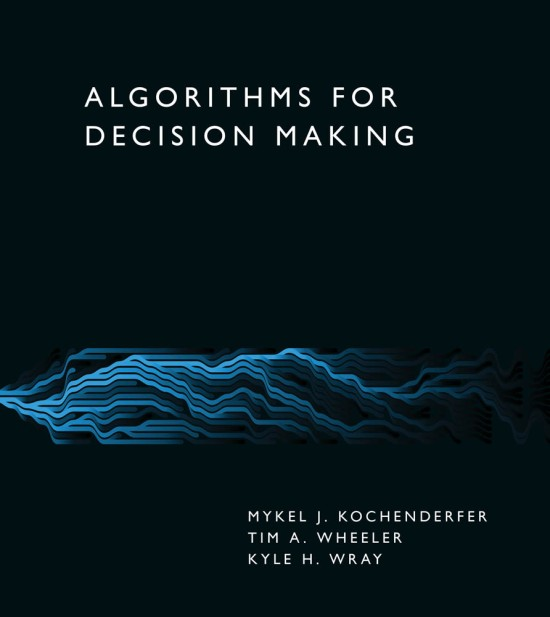
\includegraphics[width=0.5\columnwidth]{fig/book.jpg}
        \url{algorithmsbook.com/decisionmaking}
    \end{center}    
\end{frame}

\end{document}